\documentclass{article}

% --------------------------------------------------
% 基本数学与环境
% --------------------------------------------------
\usepackage{amsmath,amssymb,amsfonts,amsthm,mathtools,bm}
\usepackage{array,booktabs,longtable,multicol,multirow,makecell,tabularx,threeparttable}
\usepackage{enumitem}
\setlist[enumerate]{noitemsep, topsep=2pt}
\setlist[itemize]{noitemsep, topsep=2pt}

% --------------------------------------------------
% 版面与引用
% --------------------------------------------------
\usepackage[margin=0.9in]{geometry}
\usepackage[numbers,sort&compress]{natbib}
\usepackage[colorlinks,citecolor=purple,linkcolor=blue]{hyperref}
\usepackage{cleveref}
\usepackage{float}
\usepackage{caption,subcaption}
\usepackage{appendix}
\usepackage{authblk}
\usepackage{parskip}
\renewcommand{\baselinestretch}{1.2}

% --------------------------------------------------
% 算法环境
% --------------------------------------------------
% \usepackage[linesnumbered,boxruled,lined,commentsnumbered]{algorithm2e} % 如果只用 algorithmic，可切换掉这一行
\usepackage{algorithm,algorithmic}
\usepackage{eqparbox}
\renewcommand\algorithmiccomment[1]{\hfill\texttt{\#}\ \eqparbox{COMMENT}{\texttt{#1}}}

% 自定义 subroutine 浮动体
\usepackage{newfloat}
\newfloat{subroutine}{htbp}{los}
\floatname{subroutine}{Subroutine}
\crefname{subroutine}{subroutine}{subroutines}
\Crefname{subroutine}{Subroutine}{Subroutines}
\crefname{line}{line}{lines}
\def\algorithmautorefname{Alg.}
\Crefname{algorithm}{Alg.}{Alg.}

% --------------------------------------------------
% Theorem 环境定义
% --------------------------------------------------
\newtheorem{theorem}{Theorem}[section]
\newtheorem{lemma}[theorem]{Lemma}
\newtheorem{proposition}[theorem]{Proposition}
\newtheorem{corollary}[theorem]{Corollary}
\newtheorem{assumption}[theorem]{Assumption}
\newtheorem{condition}[theorem]{Condition}
\newtheorem{definition}[theorem]{Definition}
\newtheorem{remark}[theorem]{Remark}
\newtheorem{example}[theorem]{Example}
\newtheorem{strategy}[theorem]{Strategy}
\newtheorem{question}[theorem]{Question}
\numberwithin{equation}{section}

% cleveref 自动命名
\def\subsectionautorefname{Section}
\def\definitionautorefname{Definition}
\def\corollaryautorefname{Corollary}
\def\lemmaautorefname{Lemma}
\def\assumptionautorefname{Assumption}
\def\propositionautorefname{Proposition}
\def\tableautorefname{Table}
\def\strategyautorefname{Strategy}
\def\remarkautorefname{Remark}
\def\conditionautorefname{Condition}

% --------------------------------------------------
% TikZ & PGFPlots
% --------------------------------------------------
\usepackage{tikz,pgfplots}
\usetikzlibrary{arrows.meta,calc,backgrounds,positioning}
\usepgfplotslibrary{fillbetween,patchplots}
\pgfplotsset{compat=newest}

% 自定义颜色与样式
\definecolor{ao(english)}{rgb}{0.0,0.5,0.0}
\definecolor{cadmiumgreen}{rgb}{0.0,0.42,0.24}
\definecolor{darkpastelgreen}{rgb}{0.01,0.75,0.24}

\tikzset{
  materia/.style={draw, fill=blue!20, text width=6em, text centered, minimum height=1.5em, drop shadow},
  etape/.style={materia, text width=8em, minimum width=10em, minimum height=3em, rounded corners, drop shadow},
  linepart/.style={draw, thick, color=black!50, -Latex, dashed},
  line/.style={draw, thick, color=black!50, -Latex},
  back group/.style={fill=white!20,rounded corners, draw=black!50, dashed, inner xsep=15pt, inner ysep=10pt},
}
\newcommand{\etape}[2]{node (p#1) [etape] {#2}}
\newcommand{\transreceptor}[3]{\path [linepart] (#1.east) -- node [above] {\scriptsize #2} (#3);}

% --------------------------------------------------
% 其他常用命令
% --------------------------------------------------
\newcommand{\xk}{x_k}
\newcommand{\Hk}{H_k}
\newcommand{\gk}{g_k}
\newcommand{\dk}{d_k}
\newcommand{\xkn}{x_{k+1}}
\newcommand{\gkn}{g_{k+1}}
\newcommand{\dkn}{d_{k+1}}
\newcommand{\cmark}{\ding{51}}
\newcommand{\xmark}{\ding{55}}

% 算法名缩写
\newcommand{\arc}{\texttt{CubicReg}}
\newcommand{\arca}{\texttt{CubicReg-A}}
\newcommand{\utr}{\texttt{UTR}}
\newcommand{\utrhvp}{\texttt{UTR-HVP}}
\newcommand{\iutr}{\texttt{iUTR(Hessian)}}
\newcommand{\iutrhvp}{\texttt{iUTR}}
\newcommand{\drsom}{\texttt{DRSOM}}
\newcommand{\drsomh}{\texttt{DRSOM-H}}
\newcommand{\hsodm}{\texttt{HSODM}}
\newcommand{\hsodmarc}{\texttt{HSODMArC}}
\newcommand{\hsodmhvp}{\texttt{HSODM-HVP}}
\newcommand{\atr}{\Cref{alg.accelerated utr}}
\newcommand{\atrms}{\Cref{alg.ms accelerated utr}}
\newcommand{\tr}{\textrm{TR}}
\newcommand{\trp}{\textrm{TR}_+}
\numberwithin{equation}{section}

\author[1]{\small Yuntian Jiang}
\author[2]{\small Chuwen Zhang}
\author[1]{\small Bo Jiang\thanks{Corresponding author: isyebojiang@gmail.com}}
\author[3]{\small Yinyu Ye}


\affil[1]{\footnotesize School of Information Management and Engineering\\ Shanghai University of Finance and Economics}
\affil[2]{\footnotesize Booth School of Business\\ University of Chicago}
\affil[3]{\footnotesize Antai College of Economics and Management\\ Shanghai Jiao Tong University}

%%%%%%%%%%%%%%%%%%%%%%%%%%%%%%%%%%%%%%%%%%%%%%%%%
% \title{Homogeneous Second-Order Descent Method: Generalization and Application}
%%%%%%%%%%%%%%%%%%%%%%%%%%%%%%%%%%%%%%%%%%%%%%%%%
\title{Accelerating Trust-Region Methods: An Attempt to Balance Global and Local Efficiency}

\begin{document}

\maketitle
\begin{abstract}
    Historically speaking, it is hard to balance the global and local efficiency of second-order optimization algorithms. For instance,
    {the classical Newton's method possesses excellent local convergence but lacks global guarantees, often exhibiting divergence when the starting point is far from the optimal solution~\cite{more1982newton,dennis1996numerical}. In contrast, accelerated second-order methods offer strong global convergence guarantees, yet they tend to converge with slower local rate~\cite{carmon2022optimal,chen2022accelerating,jiang2020unified}. Existing second-order methods struggle to balance global and local performance, leaving open the question of how much we can
    globally accelerate the second-order methods while maintaining excellent local convergence guarantee. In this paper, we tackle this challenge by proposing for the first time the accelerated trust-region-type methods, and leveraging their unique primal-dual information.} Our primary technical contribution is \emph{Accelerating with Local Detection}, which utilizes the Lagrange multiplier to detect local regions and achieves a global complexity of $\tilde{O}(\epsilon^{-1/3})$, while maintaining quadratic local convergence. We further explore the trade-off when pushing the global convergence to the limit. In particular, we propose the \emph{Accelerated Trust-Region Extragradient Method} that has a global near-optimal rate of $\tilde{O}(\epsilon^{-2/7})$ but loses the quadratic local convergence.
    This reveals a phase transition in accelerated trust-region type methods: the excellent local convergence can be maintained when achieving a moderate global acceleration but becomes invalid when pursuing the extreme global efficiency.  
    Numerical experiments further confirm the results indicated by our convergence analysis.
\end{abstract}

\section{Introduction}\label{Intro}
In this paper, we consider the unconstrained convex optimization problem
\begin{equation} \label{eq.main problem}
    f^* = \min_{x\in \mathbb{R}^n} f(x),
\end{equation}
where $f:\mathbb{R}^n \to \mathbb{R}$ is a convex function.
When the Hessian of the objective is available, second-order methods (SOMs) are particularly effective for solving~\eqref{eq.main problem}, especially when high-accuracy solutions are desired. Their power stems from a central property: Newton’s method achieves quadratic convergence in a neighborhood of any non-degenerate local minimum~\cite{polyak2007newton,more1982newton,nocedal1999numerical}. Many SOMs are thus designed to approximate the Newton direction, allowing them to inherit its excellent local convergence behavior.

In addition to local convergence, another important criterion for evaluating the effectiveness of optimization methods is their non-asymptotic global oracle complexity, which refers to the number of second-order subproblems (the oracle calls) needed to find an $\epsilon$-approximate solution~\cite{cartis2022evaluation}. Over the past decades, a few SOMs have been developed with such emphases ~\cite{nesterov2006cubic,mishchenko_regularized_2023,jiang2024nonconvexityuniversaltrustregionmethod,heHomogeneousSecondorderDescent2025}.  In convex optimization, these methods can be further improved through acceleration techniques.

In this context, two major approaches have emerged. The first approach, accelerated cubic regularized Newton (CRN) method~\cite{nesterov2008accelerating}, achieves a global oracle complexity of $O(\epsilon^{-1/3})$ based on the cubic regularization oracle \cite{nesterov2006cubic}. A different strategy is adopted in the accelerated Newton proximal extragradient (A-NPE) method~\cite{monteiro2013accelerated}, which improves the oracle complexity to $\tilde{O}(\epsilon^{-2/7})$ and is compatible with second-order oracles that satisfy certain error bound conditions~\cite{carmon2022optimal}.
These developments, largely based on the estimating sequence technique~\cite{nesterovMethodSolvingConvex1983a,baesEstimateSequenceMethods2009a}, have inspired a wide range of enhancements~\cite{jiang2021optimal,chen2022accelerating,lin2022explicit,agafonov2023inexact,agafonov2024advancing,jiang2024accelerated,huang2024inexact,doikov2020contracting}.
Recently, the oracle complexity of the A-NPE method was improved to be an optimal rate in $O(\epsilon^{-2/7})$~\cite{carmon2022optimal,NEURIPS2022_e56f394b}. These acceleration techniques are broadly applicable and are by no means limited to the domain of SOMs~\cite{xu2017accelerated,xu2018accelerated,lan2012optimal,ghadimi2016accelerated}.


However,  it is hard to balance the global and local efficiency of second-order optimization algorithms. For instance,
    the classical Newton's method possesses excellent local convergence but lacks global guarantees, often exhibiting divergence when the starting point is far from the optimal solution~\cite{more1982newton,dennis1996numerical}. In contrast, stronger worst-case complexity results of accelerated SOMs often come at the cost of local efficiency.  
% While classical SOMs achieve local quadratic convergence, no existing accelerated SOM successfully retains this property. 
Empirical evidence shows that in many tasks like logistic regression, accelerated SOMs are often outperformed by unaccelerated ones~\cite{jiang2020unified,huang2024inexact,chen2022accelerating,carmon2022optimal}, and manually switching to Newton’s method is often necessary to obtain highly accurate solutions~\cite{jiang2020unified,huang2024inexact,chen2022accelerating}. The above phenomenon underscores a fundamental dilemma in accelerated SOMs, and raises the following question:
\begin{center}
    \emph{How much can we accelerate SOMs globally while maintaining their excellent local convergence?}
\end{center}

\subsection{Motivation and our approach}\label{sec.motivation}
It is folklore that the strong local performance of SOMs ultimately stems from the Newton step. Thus, to design an accelerated method with excellent local performance, the second-order oracle should have the ability to detect the local geometry near the optimal solution, providing a signal indicating that the iterates may have
entered the quadratic convergence region, allowing a Newton step to be active.
For that sake, one particular choice could be the trust-region (TR) oracle~\cite{More1983,conn2000trust}. At a given point \( x \in \mathbb{R}^n \), the classic TR oracle solves the following subproblem:
\begin{equation}
    \label{eq.classic tr subproblem}
    \begin{aligned}
        \underset{d \in \mathbb{R}^n}{\min}~ & \nabla f(x)^T d + \tfrac{1}{2} d^T \nabla^2 f(x)  d \\
        \text{s.t.}                          & \quad  \|d\| \le r,
    \end{aligned}
\end{equation}
where \( r \) denotes the trust-region radius. We denote $(d,\lambda) = \tr(x, r)$ as the primal-dual solution to this problem. For an overview of TR methods, we refer readers to two excellent monographs \cite{yuan2000review,yuan2015recent}.

Two features make \eqref{eq.classic tr subproblem} particularly appealing. Near a non-degenerate minimizer, the step reduces to the pure Newton direction once the ball constraint becomes inactive, preserving quadratic convergence, which is the capability absent from other second-order oracles. 
Moreover, \tr{} oracles can be solved in $O(n^3 + n^2\log\log(\epsilon^{-1}))$ arithmetic operations \cite{vavasisProvingPolynomialtimeSphereconstrained1990,yenewcomplexityresult1991}, incurring no significant overhead compared to solving a Newton equation.
% \footnote{In comparison, the cubic Newton oracle requires an $O\left(\log\left(1/\epsilon\right)\right)$-time 1-dimensional search procedure \cite{nesterov2006cubic,cartisChapter8Subproblem2022}.}
On the practical side, the TR oracle has been thoroughly analyzed \cite{jiangHolderianErrorBounds2022,rojasNewMatrixfreeAlgorithm2001,ho2017second,wang2022generalized}, so that highly competitive solvers have been developed \cite{rojasNewMatrixfreeAlgorithm2001, adachiSolvingTrustregionSubproblem2017, adachiEigenvaluebasedAlgorithmAnalysis2019} for it and its extensions.
To this end, TR oracles have formed the algorithmic core of general-purpose nonlinear programming solvers such as Knitro~\cite{byrd2006k}, COPT~\cite{geCardinalOptimizerCOPT2022}, and PDFO~\cite{ragonneau2024pdfo}. Similar success can be found in other cross-cutting applications ranging from adversarial training~\cite{yao2019trust} to reinforcement learning~\cite{schulman2015trust}. These advantages serve as the motivation to use \tr{} to address the global-local balance in accelerated SOMs.


However, to our best knowledge,  TR methods have not been accelerated yet as
using TR oracles introduces technical challenges. Classical TR methods cannot match the global oracle complexity of other unaccelerated SOMs~\cite{cartisComplexitySteepestDescent2010,curtis2017trust} because the dual variable $\lambda$ associated with the ball constraint in \eqref{eq.classic tr subproblem} is determined a posteriori and requires careful monitoring~\cite{curtis2018concise}. Achieving global acceleration demands relative stability between this multiplier and the step size, which roughly means that $\lambda$ should not vary too fast relative to the step size, but enforcing such stability can interfere with transitions to Newton steps near the optimum.

To address this challenge, we design, for the first time, the accelerated trust-region methods that leverage a modified TR oracle, which we call the trust-region oracle for acceleration denoted as \ref{eq.newTR}. In particular, at a point $x \in \mathbb{R}^n$, the \ref{eq.newTR} oracle solves
\begin{equation*}
\begin{aligned}
\min_{d \in \mathbb{R}^n}~ & \nabla f(x)^\top d 
    + \tfrac{1}{2} d^\top (\nabla^2 f(x) + \sigma I) d, \\
\text{s.t.} &~ \|d\| \le r.
\end{aligned}
\tag*{(TR$_+$)}
\end{equation*}
The dual variable associated with the ball constraint is denoted by $\lambda$, which can detect local geometric information of the optimal solution. 
The primal regularization $\sigma$ in \ref{eq.newTR} is used to effectively modulate $\lambda$, and maintains the stability required for global acceleration, enabling our accelerated trust-region method to systematically balance fast local convergence with provable global guarantee.
\subsection{Contribution}
This work provides an answer to the question posed earlier: we demonstrate that the compatibility between the global and local efficiency of the SOMs depends on the degree of global acceleration.
Specifically, based on the \ref{eq.newTR} oracles \cite{jiang2024nonconvexityuniversaltrustregionmethod}, we develop two accelerated TR-type methods for problem~\eqref{eq.main problem}. One can simultaneously achieve both global acceleration and quadratic local convergence, and the other has a faster global convergence rate but loses local efficiency.

The first method, \emph{Accelerated Trust-Region Method with Local Detection} (\Cref{alg.accelerated utr}), implements a local detection mechanism (\Cref{alg.local detection}) that automatically identifies and ``dives into'' the quadratic convergence regions. This design yields an improved global worst-case oracle complexity of $\tilde{O}(\epsilon^{-1/3})$, while achieving a local quadratic rate of convergence. To our best knowledge, this is the first accelerated SOM that provably achieves both $\tilde{O}(\epsilon^{-1/3})$ global oracle complexity and local quadratic convergence. 

The second method, \emph{Accelerated Trust-Region Extragradient Method} (\Cref{alg.ms accelerated utr}), is designed to persuit the limits of global performance, reaching the near-optimal global oracle complexity of $\tilde{O}(\epsilon^{-2/7})$, but loses the excellent local convergence. Thus, our analysis and experiments reveal a phase transition in accelerated trust-region type methods: pushing global efficiency to its limits naturally entails a trade-off with local performance. 
Such a phase transition occurs due to the loss of local detection in \Cref{alg.ms accelerated utr} when pursuing the near-optimal global convergence rate,
where the primal regularizer $\sigma$ is set prior to determining the extrapolation point that is used in the \ref{eq.newTR} oracle~(as in \Cref{alg.accelerated utr}).

Our theoretical findings are corroborated by numerical experiments. On a global scale, all accelerated SOMs, including ours and \cite{nesterov2008accelerating,monteiro2013accelerated}, consistently outperform the non-accelerated trust-region method~\cite{jiang2024nonconvexityuniversaltrustregionmethod} and cubic Newton method~\cite{nesterov2006cubic}. Locally, \Cref{alg.accelerated utr} exhibits quadratic convergence, and \atrms{} cannot retain superlinear convergence near the solution, similar to the empirical conclusions in \cite{carmon2022optimal,jiang2024accelerated,huang2024inexact}. These findings again confirm the necessity of local detection.

\subsection{Related works}
We review related works along two main lines: TR-type methods and accelerated SOMs that aim to achieve faster-than-sublinear efficiency. Despite the strong empirical success of TR-type methods, its theoretical analysis mainly focuses on nonconvex problems~\cite{yeSecondOrderOptimization2005,curtis2017trust,curtis2021trust,zhangHomogeneousSecondorderDescent2025,hamad2022consistently,grapiglia2015convergence,hamad2024simplepracticaladaptivetrustregion}, while  
its global complexity analysis for convex problems remains incomplete.
In fact, in convex optimization, the classical TR has worse convergence rates than other unaccelerated mainstream SOMs. This gap was recently closed in~\cite{jiang2024nonconvexityuniversaltrustregionmethod}. However, whether TR oracles can further benefit from acceleration, as achieved for other SOMs, remains an open question.

As discussed earlier, unaccelerated SOMs often exhibit superior local performance near the optimal solution compared with their accelerated counterparts. A common remedy for this issue is to employ restart strategies in accelerated frameworks~\cite{nesterov_lectures_2018}. However, this introduces a new challenge of deciding when to restart since the optimal restart frequency depends on unknown, problem-specific parameters. In contrast, when stronger global regularity conditions (akin to strong convexity) are imposed on the objective function, the restart schedule can be determined in a more structured form~\cite{ostroukhov2020tensor, lin2025perseus, huang2025approximation} or even becomes unnecessary~\cite{jiang2022generalized, marques2022variants}. Under such assumptions, these methods can accommodate global performance, and thus the intrinsic trade-off between global convergence and local efficiency becomes a secondary concern.

\paragraph{Organization of the paper}
The remaining part of this paper is organized as follows. Section~\ref{sec.priliminary} reviews the background on TR-type oracles and the use of estimate sequence techniques in accelerated second-order optimization. In Section~\ref{sec.first variant}, we present the \Cref{alg.accelerated utr}, which achieves an oracle complexity of $\tilde O(\epsilon^{-1/3})$ and exhibits quadratic convergence in high-accuracy regimes. Section~\ref{sec.second variant} introduces the \Cref{alg.ms accelerated utr}, which explores the phase transition of acceleration and attains a near-optimal oracle complexity of $\tilde O(\epsilon^{-2/7})$. Section~\ref{sec.experiments} reports numerical results on practical tasks, confirming the theoretical advantages of our proposed methods.


\section{Preliminaries}
\label{sec.priliminary}
Let $\|\cdot\|$ denote the standard Euclidean norm in $\mathbb{R}^n$, and let $x^T y$ and $\langle x,y\rangle$ represent the inner product between $x, y \in \mathbb{R}^n$. For a matrix $X \in \mathbb{R}^{n \times n}$, $\|X\|$ denotes the induced $\ell_2$ norm.
% We use the standard notations $O(\cdot), \Omega(\cdot), \Theta(\cdot)$ in their conventional sense, where $\tilde{O}(\cdot)$ hides logarithmic terms within $O(\cdot)$. Specifically, for two numerical quantities $A$ and $B$, we say that $A = O(B)$ if there exists an absolute constant $c > 0$ such that $A \leq c \cdot B$, and $A = \Omega(B)$ if there exists an absolute constant $c > 0$ such that $A \geq c \cdot B$. We write $A = \Theta(B)$ if both $A = O(B)$ and $A = \Omega(B)$ hold.
Unless otherwise stated, all logarithmic functions $\log(x)$ in this paper refer to the base-2 logarithm.

We are interested in finding $\epsilon$-approximate solutions of \eqref{eq.main problem} defined as below.
\begin{definition}
    \label{def.approximate solution}
    Given $0<\epsilon <1$, a point $x \in \mathbb{R}^n$ is an $\epsilon$-approximate solution to problem~\eqref{eq.main problem} if
    \begin{equation}
        \label{eq.approximate solution}
        f(x) - f^* \leq \epsilon \quad \text{or} \quad \|\nabla f(x)\| \leq \epsilon.
    \end{equation}
\end{definition}
The following assumptions are used throughout the paper. Some of them are invoked only when necessary and will be stated explicitly.
\begin{assumption}
    \label{assm.lipschitz}
    The objective function $f: \mathbb{R}^n \to \mathbb{R}$ is twice continuously differentiable, and its Hessian is Lipschitz continuous. That is, there exists a constant $M > 0$ such that for all $x, y \in \mathbb{R}^n$,
    \begin{equation}
        \label{eq.main assm}
        \|\nabla^2 f(x) - \nabla^2 f(y)\| \leq M \|x - y\|. \end{equation}
\end{assumption}
\begin{assumption}
    \label{assm.solvable}
    The problem \eqref{eq.main problem} is solvable; that is, there exists $x^* \in \mathbb{R}^n$ such that
    \begin{equation*}
        f(x^*) = f^*:= \min_{x \in \mathbb{R}^n} f(x).
    \end{equation*}
\end{assumption}
\begin{assumption}
    \label{assm.bounded hessian}
    The Hessian of the objective function is bounded. That is, there exists a constant $\kappa_H > 0$ such that for all $x \in \mathbb{R}^n$, \begin{equation}
        \label{eq.bounded hessian}
        \|\nabla^2 f(x)\| \leq \kappa_H.
    \end{equation}
\end{assumption}
As a direct consequence of Assumption~\ref{assm.lipschitz}, we have
\begin{lemma}[Lemma 4.1.1, \citet{nesterov_lectures_2018}]\label{lem.lipschitz}
    If \(f:\mathbb{R}^n \mapsto \mathbb{R}\) satisfies Assumption~\ref{assm.lipschitz}, then for all \(x,y\in \mathbb{R}^n\), we have
    \begin{subequations}
        \begin{align}
            \label{eq.first-order exp}
             & \left\|\nabla f(y)-\nabla f(x)-\nabla^{2} f(x)(y-x)\right\|                       \leq \frac{M}{2}\|y-x\|^{2} \\
            \label{eq.second-order exp}
             & \left|f(y)-f(x)-\nabla f(x)^T(y-x)-\frac{1}{2}(y-x)^T\nabla^{2} f(x)(y-x)\right|  \leq \frac{M}{6}\|y-x\|^{3}.
        \end{align}
    \end{subequations}
\end{lemma}

To proceed, let us introduce a unified view of the updates of SOMs. In fact, almost all of the SOMs choose the step $d$ at a given point $x$ as
\begin{equation}
    \label{eq.second-order update}
    \left (\nabla^2 f(x) + \mu I \right )d = -\nabla f(x).
\end{equation}
The regularization parameter $\mu$ plays a critical role in the convergence analysis and varies among different SOMs. For example, in the classical TR method using the standard oracle~\eqref{eq.classic tr subproblem}, $\mu$ is fully determined as a posteriori, and is exactly the Lagrangian multiplier associated with the ball constraint in \eqref{eq.classic tr subproblem}. In the regularized Newton methods~\cite{mishchenko_regularized_2023}, $\mu$ can be explicitly selected as $\Theta(\sqrt{\|\nabla f(x)\|})$ such that a $O(\epsilon^{-1/2})$ method can be designed . In the CRN method~\cite{nesterov2006cubic}, it requires some search procedures on $\mu$. 

The following lemmas clarify $\mu$ plays an important role in the convergence analysis of SOMs, the proofs of which can be found in \Cref{sec.proof pre}.
\begin{lemma}
    \label{lem.bound next gradient}
    Suppose Assumption~\ref{assm.lipschitz} and \eqref{eq.second-order update} hold, then we have
    \begin{equation}
        \label{eq.bound next gradient}
        \|\nabla f(x+d)\| \leq \frac{M}{2}\|d\|^2+\mu\|d\|.
    \end{equation}
\end{lemma}

\begin{lemma}
    \label{lem.inner product g and d}
    Suppose Assumption~\ref{assm.lipschitz} and \eqref{eq.second-order update} hold,
    holds for some $\mu$ with $\mu\geq M \|d\|$, then we have
    \begin{equation}
        \label{eq.inner product g d}
        \langle \nabla f(x+d),-d \rangle \geq \frac{\|\nabla f(x+d)\|^2}{2\mu}+\frac{3}{8}\mu \|d\|^2.
    \end{equation}
    Further, if $\mu \leq 2M\|d\|$, we have
    \begin{equation}
        \label{eq.inner product g d advanced}
        \langle \nabla f(x+d),-d \rangle \geq \frac{\sqrt{6}}{6} \frac{\|\nabla f(x+d)\|^{3/2}}{\sqrt{M}}.
    \end{equation}
\end{lemma}

Generally speaking, \Cref{lem.bound next gradient} shows that we can bound the next-iterate gradient norm by controlling $\mu$.
{\Cref{lem.inner product g and d} serves as a key bridge to establish the global efficiency~(in fact, it is a modified version of~\cite[Lemma 4.2.5]{nesterov_lectures_2018} and~\cite[Corollary 1]{nesterovImplementableTensorMethods2021} for TR-type oracle)}, which suggests that $\mu$ should be selected roughly as $\Theta(\|d\|)$. This condition generally fails for the classical TR oracle, as explained in~\Cref{sec.motivation} and also discussed in~\cite{curtis2018concise,curtis2017trust}. For this reason, we adopt the \ref{eq.newTR} oracle:
% However, achieving this global-local balance is far from straightforward. On one hand, the multiplier in standard TR oracles is not stable and is determined a posteriori, making it difficult to consistently satisfy $\mu = \Theta(\|d\|)$ required by persueing better global complexity. On the other hand, existing accelerated SOMs often lack local detection mechanisms and therefore tend to adopt globally conservative strategies by default. As a result, their local steps remain overly cautious even when faster convergence is possible.
\begin{equation}\label{eq.newTR}
\begin{aligned}
    \min_{d \in \mathbb{R}^n}~ & \nabla f(x)^T d 
    + \tfrac{1}{2} d^T (\nabla^2 f(x) + \sigma I) d, \\
    \text{s.t.} &~ \|d\| \le r,
\end{aligned}
\tag*{(TR$_+$)}
\end{equation}
We denote $(d, \lambda) = \trp(x, \sigma, r)$ as the primal-dual solution of the \ref{eq.newTR} subproblem, and in the following, all references to solution pairs $(d,\lambda)$ will refer to this \ref{eq.newTR} solution unless otherwise stated.
The global optimality conditions are as follows.
\begin{lemma}[Section 3,~\citet{conn2000trust}]\label{lem.optimal condition}
    The direction $d$ is the solution to \ref{eq.newTR} if and only if there exists a dual multiplier $\lambda \geq 0$ such that: \begin{subequations}\label{eq.sa}
        \begin{align}
            \label{eq.optcond primal}
             & \| d\| \leq r                                                       \\
            \label{eq.optcond coml slack}
             & \lambda \left(\|d\|-r \right)=0                                     \\ \label{eq.optcond firstorder}
             & \left(\nabla^2 f(x) + \sigma I + \lambda I \right) d = -\nabla f(x) \\
            \label{eq.optcond secondorder}
             & \nabla^2 f(x) + \sigma I + \lambda I \succeq 0.
        \end{align}
    \end{subequations}
\end{lemma}
In the \ref{eq.newTR} oracle, the regularization parameter decomposes as $\mu=\sigma+\lambda$, aggregating \emph{a prior} regularizer from the primal problem and \emph{a posterior} dual variable. As we will show in the following, this primal-dual combo of information has the potential to balance global and local behavior.
\section{Variant~I: Balancing the Global-Local Trade-off}\label{sec.first variant}
In this section, we propose the first accelerated TR method, which applies the primal-dual structure of \ref{eq.newTR} into the estimating sequence \cite{nesterov2008accelerating}. The global oracle complexity is improved to $\tilde O(\epsilon^{-1/3})$ as opposed to the recent $O(\epsilon^{-1/2})$ in convex optimization \cite{jiang2024nonconvexityuniversaltrustregionmethod}, while the local rate of convergence to the non-degenerate solution remains quadratic.
\subsection{Algorithm design}
\Cref{alg.accelerated utr} and its local detection mechanism (\Cref{alg.local detection}) are presented below.
\begin{algorithm}[ht]
    \caption{Accelerated Trust-Region Method with Local Detection (\atr{})}\label{alg.accelerated utr}
    \begin{algorithmic}[1]
        \STATE \textbf{input:} initial point $x_0=v_0\in \mathbb{R}^n$, $s_0=0$, tolerance $\epsilon>0$
        \FOR{$k=0, 1, \ldots, K_\epsilon$}
        \STATE $y_k = \frac{k}{k+3}x_k+\frac{3}{k+3}v_k$
        \STATE $(\sigma_k,r_k) = (\tfrac{\sqrt{2M}}{2}\|\nabla f(y_k)\|^{1/2},\tfrac{1}{\sqrt{2M}}\|\nabla f(y_k)\|^{1/2})$
        \STATE $(d_k,\lambda_k) = \trp(y_k,\sigma_k,r_k)$ 
        % \noindent\rule{8cm}{0.4pt} 
        \IF{$\lambda_k=0$} \label{line.if}
        % \STATE $x_{k+1}=y_k+d_k$ \label{line.nonzero multiplier}
        \STATE \texttt{\# Enter Local Detection (\Cref{alg.local detection})}
        % \STATE $z_i,\text{ET}=\operatorname{Newton}(y_k,\left \lceil\frac{\log \|\nabla f(y_k)\|}{\epsilon} \right\rceil)$ 
        % \STATE $(z_i,d_k,\mu_k,\text{ET}) = \operatorname{LD}(y_k,\tfrac{\sqrt{2M}}{2}\|\nabla f(y_k)\|^{1/2},d_k,\epsilon)$
        \STATE $(x_{k+1},\text{ET}) = \operatorname{LD}(y_k,\tfrac{\sqrt{2M}}{2}\|\nabla f(y_k)\|^{1/2},d_k,\epsilon)$
        \label{line.early terminate main}
        \IF{$\text{ET}$}
        \STATE \textbf{terminate and output $x_{k+1}$}
        \ENDIF
        % \IF{$\textrm{ET}$} \STATE\textbf{terminate} \ENDIF
        \ENDIF
        % \STATE $x_{k+1}=y_k+d_k$
        \STATE $s_{k+1} = s_{k}+\tfrac{(k+1)(k+2)}{2}\nabla f(x_{k+1})$
        \STATE $v_{k+1} = v_0-\sqrt{\tfrac{8}{3M\|s_{k+1}\|}}s_{k+1}$
        \ENDFOR
    \end{algorithmic}
\end{algorithm}
\begin{subroutine}[!ht]
    \caption{Local Detection (LD) }\label{alg.local detection}
    \begin{algorithmic}[1]
        \STATE{\textbf{input:} $z_0=y\in \mathbb{R}^n$, $\mu_+$, $d_+$, $\epsilon$;
            \label{line.right bracket point}
        }
        \IF{$\|d_+\| \leq \min\{\frac{\epsilon}{2\kappa_H}, \sqrt{\frac{\epsilon}{M}}\}$}\label{line.if coro 3.1}
        \STATE{\textbf{output} $y+d_+$, ET =True
            \label{line.et 2}
        }
        \ENDIF
        \STATE{\texttt{\# Track 1: Local Diving}}
        \FOR{$i=1,\ldots,\left \lceil\log\frac{\|\nabla f(y)\|}{\epsilon} \right\rceil$}\label{line.track 1 number of iter}
        \STATE{$z_i = z_{i-1}-\nabla^2f(z_{i-1})^{-1}\nabla f(z_{i-1})$}
        \IF{$\|\nabla f(z_i)\|\leq \epsilon$}
        \STATE{\textbf{output} $z_i$, ET=True
            \label{line.et 1}
        }
        \ENDIF
        \ENDFOR
        \STATE{\texttt{\# Track 2: Ratio Bracketing and Bisection~(R\&B)}}
        \IF{$\frac{\mu_+}{\|d_+\|}\leq 2M$
            \label{line.check right bracket point}}
        \STATE{\textbf{output} $y+d_+$, ET =False
            \hfill\texttt{\# Check if the bisection is needed}
        }
        \ELSE
        \STATE{$r_- = \|d_+\|$, $r_+ = \left \|\left(\nabla^2f(y)+M\|d_+\| I\right)^{-1}\nabla f(y)\right\|$
            \label{line.left bracketing point}
        }
        \ENDIF
        \WHILE{True}
        \STATE{$r = \tfrac{r_-+r_+}{2}$
        \hfill\texttt{\# Perform bisection over $r \in [r_-, r_+]$}
        }
        \STATE{$(d,\mu) = \trp(y,0,r)$
        \label{line.linear system oracle}
        }
        \IF{$\frac{\mu}{\|d\|}<M$}
        \STATE{$r_+=r$}
        \ELSIF{$\tfrac{\mu}{\|d\|}>2M$}
        \STATE{$r_- = r$}
        \ELSE
        \STATE{\textbf{output} $y + d$, ET= False}
        \ENDIF
        \ENDWHILE
        % \WHILE{$\frac{\mu}{\|d\|} \not\in [M, 2M]$}
        % \STATE{Perform bisection over $r \in [r_-, r_+]$}
        % \hfill\texttt{\# Bisection starts}

        % \STATE{$(d,\mu) = \trp(y,0,r)$
        %     \label{line.linear system oracle}
        % }
        % % \IF{$\frac{\mu}{\|d\|}<M$}
        % % \STATE{$r_+=r$}
        % % \ELSIF{$\tfrac{\mu}{\|d\|}>2M$}
        % % \STATE{$r_- = r$}
        % % \ELSE
        % % \STATE{\textbf{output} None, $d$, $\mu$, ET= False}
        % % \ENDIF
        % \ENDWHILE
        % \STATE{\textbf{output} None, $d$, $\mu$, ET= False}
        % \STATE{\textbf{output} $y + d$, ET= False}

    \end{algorithmic}
\end{subroutine}
The overall regularization in \ref{eq.newTR} is a combination of primal and dual information: $\mu_k = \sigma_k + \lambda_k$. The primal part $\sigma_k$ is chosen carefully to make the dual part more stable and still carry local information, while the dual part $\lambda_k$ is used as an indicator to check whether the current iterate is close to the local optimum according to the value of $\lambda_k$.

% The algorithm proceeds by checking whether the dual multiplier $\lambda_k$ is zero.

The case $\lambda_k > 0$ typically indicates that the current iterate is still far from a local optimum. In that regime, as shown later in \Cref{lem.ratio pass nonzero}, the overall regularization parameter $\mu_k$ becomes automatically proportional to the step size, which justifies the updates of the estimating sequence in the acceleration framework.

The case $\lambda_k = 0$ is a signal that the current extrapolation point $y_k$ may have entered the local quadratic convergence region of Newton's method (see \Cref{lem.detection of local quadratic}). This triggers the Local Detection procedure (LD, \Cref{alg.local detection}), which consists of two separate tracks named local diving and R\&B respectively probing the local geometry around $y_k$. 

In local diving (\texttt{Track 1}), we run Newton's method starting from $y_k$, the resulting sequence is indexed by $i$ and denoted by $\{z_i\}$. As discussed in Section~\ref{sec.local}, if $y_k$ indeed lies within the quadratic convergence region, the resulting sequence $\{z_i\}$ will exhibit quadratic convergence, which justifies early termination of \Cref{alg.accelerated utr}.~(In practice, we could stop diving if the $\|\nabla f(z_i)\|$ is not decreasing, or a degenerate Hessian is detected.)

In R\&B (\texttt{track 2}), we attempt to find a step $d_k$ whose size is proportional to the regularization parameter $\mu_k$. This step certifies the updates of the estimate sequence and thus preserves global acceleration. 

In summary, \Cref{alg.accelerated utr} admits two possible termination routes: when $y_k$ enters the region of local quadratic convergence, the algorithm detects this and terminates early with ET$=$True~(see lines~\ref{line.et 2} and \ref{line.et 1} in \Cref{alg.local detection}). Otherwise, it continues to follow a path of globally accelerated sequences with $\mathrm{ET} = \mathrm{False}$.

\subsection{Global complexity analysis}
Now we analyze the worst-case global oracle complexity of \Cref{alg.accelerated utr} for computing an approximate solution as defined in \Cref{def.approximate solution}. Since our goal here is to analyze the worst-case global complexity, we assume the iterates do not step into local diving of \Cref{alg.local detection}, which is more relevant to local convergence analysis (cf. \Cref{sec.local}). Our analysis follows a standard procedure: we first establish the \textit{iteration complexity} of the accelerated sequence in~\Cref{alg.accelerated utr}, and subsequently determine the number of oracle calls required per iteration in~\Cref{alg.local detection}, thereby obtaining the final \textit{oracle complexity} bound.
\subsubsection{Iterations complexity of \Cref{alg.accelerated utr}}
Denote $K_\epsilon$ as the iteration number \Cref{alg.accelerated utr} takes to find an approximate solution satisfying \eqref{eq.approximate solution}. We show $K_\epsilon = O(\epsilon^{-1/3})$.

When using the estimating sequence technique in~\cite{nesterov2008accelerating}, the globally accelerated convergence is guaranteed by maintaining the following two relations across iterations
\begin{subequations}\label{eq.es relation}
    \begin{align}
        \label{eq.es relation 1}
         & \phi_k^*  \geq A_k f(x_k), \  \phi_k^*= \phi_k(v_k) =\min_{x\in\mathbb{R}^n}\phi_k(x) \\
        \label{eq.es relation 2}
         & \phi_k(x)\leq A_kf(x)+\phi_0(x), \ \forall x\in\mathbb{R}^n.
    \end{align}
\end{subequations}
Here $\{\phi_k(x)\}_{k\geq 0}$ is a sequence of functions that approximate $f(x)$ from both above and below with $\{v_k\}_{k\geq0}$ being the optimum, $\{A_k\}_{k\geq 0}$ is a sequence that measures the convergence rate of the sequence $\{x_k\}_{k\geq 0}$. As a result of \eqref{eq.es relation}, we have
\begin{equation*}
    f(x_k)-f(x)\leq \frac{1}{A_k}\phi_0(x), \ \forall x\in \mathbb{R}^n.
\end{equation*}
Therefore, the global complexity directly follows from the choice of $A_k$ and $\phi_0(x)$.

For the upcoming analysis, we first complete the definition of $A_k,\phi_k(x)$ in the estimating sequence framework that was not explicitly presented in the algorithm:
\begin{equation}
    \label{eq.update a and A}
    a_k = \frac{(k+1)(k+2)}{2}, \ A_k=\frac{k(k+1)(k+2)}{6},
\end{equation}
\begin{align}\label{eq.update phi}
    \phi_0(x) = \frac{M}{8}\|x-x_0\|^3, \ \phi_{k+1}(x) =\phi_k(x)+a_k\left (f(x_{k+1})+\langle \nabla f(x_{k+1}),x-x_{k+1}\rangle \right ).
\end{align}
Here are some basic properties of the estimating sequence, which are from \citet{nesterov_lectures_2018}.
\begin{lemma}
    \label{lem.magnitude a and A}
    For $k\geq 0$, we have
    \begin{equation}
        \label{eq.magnitude a and A}
        \frac{A_{k+1}}{a_k^{3/2}} \geq \frac{\sqrt{2}}{3}.
    \end{equation}
\end{lemma}
\begin{proof}The conclusion follows from that
    $$\frac{A_{k+1}}{a_k^{3/2}}= \frac{(k+1)(k+2)(k+3)}{6}\cdot \frac{2^{3/2}}{(k+1)^{3/2}(k+2)^{3/2}} = \frac{\sqrt{2}(k+3)}{3(k+1)^{1/2}(k+2)^{1/2}} \geq \frac{\sqrt{2}}{3}.$$
\end{proof}
We call a differentiable function $d(x)$ on $\mathbb{R}^n$ uniformly convex \cite[Section 4.2.2]{nesterov_lectures_2018} of degree $p\geq 2$ with constant $q>0$ if
\begin{equation}
    \label{eq.uniformly convex of p}
    d(y)\geq d(x)+\langle \nabla d(x),y-x\rangle +\frac{q}{p}\|y-x\|^p, \ \forall x,y\in\mathbb{R}^n.
\end{equation}
\begin{lemma}
    \label{lem.property of phi}
    For the function sequence $\phi_k(x)$, they have the following properties
    \begin{enumerate}
        \item $\phi_k(x)$ is uniformly convex of degree $3$ with constant $\frac{3M}{16}$.
        \item $v_k$ is the unique minimizer of $\phi_k(x)$, and
              \begin{equation}
                  \label{eq.phi_k phi_low}
                  \phi_k(x)\geq \phi_k^* + \frac{M}{16}\|x-v_k\|^3.,
              \end{equation}
              where $\phi_k^* =\min \phi_k(x).$
    \end{enumerate}
\end{lemma}
\begin{proof}
    The first claim is from the definition of $\phi_0$ in \eqref{eq.update phi}, for analysis of uniform convex functions, please refer to \cite[Section 4.2.2]{nesterov_lectures_2018}. For the second claim, we have
    \begin{equation}
        \label{eq.phi recursive}
        \phi_k(x) = \phi_0(x)+\sum_{i=0}^{k-1}a_i\left (f(x_{i+1})+\langle \nabla f(x_{i+1}),x-x_{i+1}\rangle \right).
    \end{equation}
    From the optimality condition, we have that
    \begin{equation*}
        \begin{aligned}
            \nabla \phi_k(x) & = \nabla \phi_0(x)+ \sum_{i=0}^{k-1} a_i\nabla f(x_{i+1})                \\
                             & = \frac{3M}{8}\|x-x_0\|(x-x_0)+\sum_{i=0}^{k-1} a_i\nabla f(x_{i+1}) =0.
        \end{aligned}
    \end{equation*}
    Solving the optimality condition and noticing the way we update $s_k$ gives
    \begin{equation*}
        x = v_0 - \sqrt{\frac{8}{3M\|s_{k}\|}}s_{k},
    \end{equation*}
    which is $v_k$. Then \eqref{eq.phi_k phi_low} holds from the fact that $\phi_k(x)$ is uniformly convex of degree 3.
\end{proof}
To proceed, we categorize the iterates generated by \Cref{alg.accelerated utr} into two disjoint sets based on the value of the multiplier, according to whether the iterations invoke local detection:
\begin{equation}
    \label{eq.outer index catagory}
    \begin{aligned}
         & \mathcal{Z} = \left \{k |k\leq K_\epsilon,\ \lambda_k=0\right\},   \\
         & \mathcal{N} = \left \{ k | k\leq K_\epsilon,\ \lambda_k>0\right\}.
    \end{aligned}
\end{equation}
We first demonstrate that the ratio between the regularizer and the step size remains stable for $k\in\mathcal{N}$ as shown in \eqref{eq.output of alg2} which exhibits the power of \ref{eq.newTR}. 
\begin{lemma}
    \label{lem.ratio pass nonzero}
    In the $k$-th iteration of \Cref{alg.accelerated utr}, if $k\in\mathcal{N}$, then
    \begin{subequations}
        \label{eq.output of alg2}
        \begin{gather}
            d_k = -\left(\nabla^2 f(y_k)+\mu_k I \right)^{-1}\nabla f(y_k)\\
            M\|d_k\|\leq \mu_k \leq 2M\|d_k\|.
        \end{gather}
    \end{subequations}
\end{lemma}
\begin{proof}
    On the one hand, by our choice of $(\sigma_k,r_k)$, we have $$\mu_k=\sigma_k+r_k\geq\sigma_k= Mr_k= M\|d_k\|.$$
    On the other hand, since $\nabla^2 f(y_k)\succeq 0$, we have
    \begin{equation*}
        \mu_k\|d_k\|=\|\mu_kd_k\|\leq \left\|\left(\nabla^2 f(y_k)+\mu_k I\right)d_k\right\|=\|\nabla f(y_k)\|.
    \end{equation*}
    Note that $\lambda_k>0$ implies $\|d_k\|=r_k=\frac{1}{\sqrt{2M}}\|\nabla f(y_k)\|$. As a result, we have
    \begin{equation*}
        \mu_k\leq \frac{\|\nabla f(y_k)\|}{\|d_k\|}=\sqrt{2M}\|\nabla f(y_k)\|=2M\|d_k\|.
    \end{equation*}
    Therefore, \eqref{eq.output of alg2} holds.
\end{proof}
To maintain the flow of the complexity analysis, we temporarily assume the output of R\&B of \Cref{alg.local detection} satisfies~\eqref{eq.output of alg2} as well, i.e., \eqref{eq.output of alg2} holds for $k\in\mathcal{Z}$~(we will rigorously verify this later). Now we are able to show that, during the update of \Cref{alg.accelerated utr}, the relation \eqref{eq.es relation} holds.
\begin{lemma}\label{lem.estimate sequence}
    Suppose Assumption~\ref{assm.lipschitz} holds, and \eqref{eq.output of alg2} holds for the output of \Cref{alg.local detection}. Then we can guarantee the following for all $k\geq 0$:
    \begin{equation}
        \label{eq.estimating sequence relation}
        A_k f(x_k)\leq \phi_k^*  \leq \phi_k(x)\leq A_k f(x)+\phi_0(x), \ \forall x\in \mathbb{R}^n.
    \end{equation}
\end{lemma}
\begin{proof}
    We conduct the proof by induction. Note that $A_0 = 0$, so \eqref{eq.estimating sequence relation} holds for $i=0$. Suppose it also holds for $i=k$.
    We first check \eqref{eq.es relation 2} for $i=k+1$:
    \begin{align*}
        \phi_{k+1}(x) & =\phi_k(x)+a_k\left(f(x_{k+1})+\langle \nabla f(x_{k+1}),x-x_{k+1}\rangle \right)               \\
                      & \leq A_k f(x)+\phi_0(x) +a_k\left(f(x_{k+1})+\langle \nabla f(x_{k+1}),x-x_{k+1}\rangle \right) \\
                      & \leq A_k f(x)+\phi_0(x) +a_k f(x)                                                               \\
                      & =A_{k+1} f(x)+\phi_0(x),
    \end{align*}
    where the first inequality is from the induction hypothesis.
    We now check \eqref{eq.es relation 1} for $i=k+1$,
    \begin{align*}
        \phi_{k+1}^*
         & = \min_{x\in\mathbb{R}^n} \left\{ \phi_k(x) + a_k \left(f(x_{k+1}) + \langle \nabla f(x_{k+1}), x - x_{k+1} \rangle \right) \right\} \\
         & \geq \min_{x\in\mathbb{R}^n} \Bigl\{ \phi_k^* + \frac{M}{16} \|x - v_k\|^3
        + a_k \left(f(x_{k+1}) + \langle \nabla f(x_{k+1}), x - x_{k+1} \rangle \right) \Bigr\}                                                 \\
         & \geq \min_{x\in\mathbb{R}^n} \Bigl\{ A_k f(x_k) + \frac{M}{16} \|x - v_k\|^3
        + a_k \left(f(x_{k+1}) + \langle \nabla f(x_{k+1}), x - x_{k+1} \rangle \right) \Bigr\}                                                 \\
         & \geq \min_{x\in\mathbb{R}^n} \Bigl\{ A_k f(x_{k+1}) + A_k \langle \nabla f(x_{k+1}), x_k - x_{k+1} \rangle                           \\
         & \qquad + \frac{M}{16} \|x - v_k\|^3 + a_k \left(f(x_{k+1}) + \langle \nabla f(x_{k+1}), x - x_{k+1} \rangle \right) \Bigr\}          \\
         & =  A_{k+1} f(x_{k+1})
        + A_{k+1} \left\langle \nabla f(x_{k+1}),
        \frac{A_k}{A_{k+1}} x_k + \frac{a_k}{A_{k+1}} v_k - x_{k+1} \right\rangle                                                               \\
         & \qquad + \min_{x\in\mathbb{R}^n} \Bigl\{\frac{M}{16} \|x - v_k\|^3
        + a_k \langle \nabla f(x_{k+1}), x - v_k \rangle \Bigr\}                                                                                \\
         & = A_{k+1} f(x_{k+1})
        + A_{k+1} \left\langle \nabla f(x_{k+1}),
        \frac{A_k}{A_{k+1}} x_k + \frac{a_k}{A_{k+1}} v_k - x_{k+1} \right\rangle                                                               \\
         & \qquad - \frac{a_k^{3/2}}{3\sqrt{3} \cdot \sqrt{M}} \|\nabla f(x_{k+1})\|^{3/2}                                                      \\
         & = A_{k+1} f(x_{k+1}) + A_{k+1} \langle \nabla f(x_{k+1}), y_k - x_{k+1} \rangle
        - \frac{a_k^{3/2}}{3\sqrt{3} \cdot \sqrt{M}} \|\nabla f(x_{k+1})\|^{3/2}                                                                \\
         & = A_{k+1} f(x_{k+1}) + A_{k+1} \left(
        \langle \nabla f(x_{k+1}), y_k - x_{k+1} \rangle
        - A_{k+1}^{-1} \cdot \frac{a_k^{3/2}}{3\sqrt{3} \cdot \sqrt{M}}
        \|\nabla f(x_{k+1})\|^{3/2} \right)                                                                                                     \\
         & \geq A_{k+1} f(x_{k+1}) + A_{k+1} \left(
        \langle \nabla f(x_{k+1}), y_k - x_{k+1} \rangle
        - \frac{\sqrt{6}}{6\sqrt{M}} \|\nabla f(x_{k+1})\|^{3/2} \right).
    \end{align*}
    In the above analysis, the first inequality is because of the uniform convexity of $\phi_k$, the second inequality is from the induction hypothesis, the third inequality is from the convexity of $f$, and the last inequality is from \eqref{eq.magnitude a and A}. Now it reduces to proving
    \begin{equation*}
        \langle f(x_{k+1}),y_k-x_{k+1} \rangle -\frac{\sqrt{6}}{6\sqrt{M}}\|\nabla f(x_{k+1})\|^{3/2} \geq 0.
    \end{equation*}
    Note that we have
    \begin{equation*}
        M\|d_k\| \leq \mu_k \leq 2M\|d_k\|.
    \end{equation*}
    As a result of \eqref{eq.inner product g d advanced}, it holds that
    \begin{equation*}
        \langle f(x_{k+1}),y_k-x_{k+1} \rangle -\frac{\sqrt{6}}{6\sqrt{M}}\|\nabla f(x_{k+1})\|^{3/2} \geq 0.
    \end{equation*}
    Thus the proof is complete.
\end{proof}
As a direct consequence of \eqref{eq.update a and A} and \Cref{lem.estimate sequence}, we have the following global iteration complexity result of \Cref{alg.accelerated utr}.
\begin{theorem}
    \label{thm.convergence outer loop}
    Suppose Assumption~\ref{assm.lipschitz} and Assumption~\ref{assm.solvable} hold, and \eqref{eq.output of alg2} holds for the output of \Cref{alg.local detection}, then \Cref{alg.accelerated utr} finds a point $x\in\mathbb{R}^n$ that satisfies \eqref{eq.approximate solution} in $K_\epsilon=O(\epsilon^{-1/3})$ iterations.
\end{theorem}

\subsubsection{Oracle complexity of \Cref{alg.local detection}}
It remains to analyze how many oracles are needed in R\&B to find a direction that satisfies \eqref{eq.output of alg2}. We will show that the number of \ref{eq.newTR} oracles needed is bounded above by $O(\log\tfrac1\epsilon)$. As the argument is quite technical, some of the proofs are postponed to \Cref{sec.proof variant 1}.

We begin with the following property of the iterates $y_k$ with $k\in\mathcal{Z}$.
\begin{lemma}
    \label{lem.upper bound for zero lambda}
    Suppose Assumption~\ref{assm.bounded hessian} hold, for $k\in \mathcal{Z}$, we have
    \begin{equation}
        \label{eq.upper bound for zero lambda}
        \|\nabla f(y_k)\|\leq \frac{2\kappa_H^2}{M}.
    \end{equation}
\end{lemma}
\begin{proof}
    Note that when $k\in \mathcal{Z}$, we have $\lambda_k =0$, hence the following hold
    \begin{equation*}
        \left (\nabla^2 f(y_k)+\frac{\sqrt{2M}}{2}\|\nabla f(y_k)\|^{1/2} I\right )d_+ = -\nabla f(y_k), \ \|d_+\| \leq \frac{1}{\sqrt{2M}}\|\nabla f(y_k)\|^{1/2}.
    \end{equation*}
    Therefore, by the triangle inequality, it holds that
    \begin{equation*}
        \|\nabla f(y_k)\| \leq \|\nabla^2 f(y_k) d_+\| +\frac{\sqrt{2M}}{2}\|\nabla f(y_k)\|^{1/2}\|d_+\| \leq \|\nabla^2 f(y_k) d_+\|+\frac{1}{2}\|\nabla f(y_k)\|.
    \end{equation*}
    By Assumption~\ref{assm.bounded hessian}, we have
    \begin{equation*}
        \begin{aligned}
            \kappa_H \cdot \frac{1}{\sqrt{2M}}\|\nabla f(y_k)\|^{1/2}  \geq \kappa_H \|d_+\|  & \geq \|\nabla^2 f(y_k) d_+\|       \geq \frac{1}{2}\|\nabla f(y_k)\|.
        \end{aligned}
    \end{equation*}
    By rearranging terms, we obtain \eqref{eq.upper bound for zero lambda}.
\end{proof}
\begin{corollary}
    \label{coro.second et}
    Suppose Assumption~\ref{assm.lipschitz}, Assumption~\ref{assm.bounded hessian}, and the "if" condition $\|d_+\|\leq \min\{\frac{\epsilon}{2\kappa_H},\sqrt{\frac{\epsilon}{M}}\}$ at line~\ref{line.if coro 3.1} of \Cref{alg.local detection} hold, then we have
    \begin{equation*}
        \|\nabla f(y+d_+)\|\leq \epsilon.
    \end{equation*}
\end{corollary}
\begin{proof}
    From \Cref{lem.bound next gradient}, we have
    \begin{equation*}
        \begin{aligned}
            \|\nabla f(y+d_+)\| & \leq \frac{M}{2}\|d_+\|^2 + \frac{\sqrt{2M}}{2}\|\nabla f(y)\|^{1/2}\|d_+\|                                                          \\
                                & \leq \frac{M}{2}\times \frac{\epsilon}{M}+\frac{\sqrt{2M}}{2}\times\frac{\sqrt{2}\kappa_H}{\sqrt{M}}\times\frac{\epsilon}{2\kappa_H} \\
                                & \leq \epsilon.
        \end{aligned}
    \end{equation*}
\end{proof}
This implies that, in the subsequent analysis, we may assume that $\|d_+\| > \min\{\frac{\epsilon}{2\kappa_H},\sqrt{\frac{\epsilon}{M}}\}$. Otherwise, an approximate solution has already been found.

Now we focus on the oracle complexity of R\&B, i.e., the complexity of bisection over radius $r$ on the interval $[r_-,r_+]$ to make \eqref{eq.output of alg2} hold. For simplicity, we omit the subscript $k$ in the analysis of the bisection procedure. In each step of the bisection, the update $(d,\mu)=\trp(y,0,r)$ with $r\in[r_-,r_+]$ defines the correspondence between $r$ and $\mu$ over the interval $[r_-,r_+]$ and $[\mu_-,\mu_+]$, where $\mu_-$ and $\mu_+$ have the following value due to the mechanism of \Cref{alg.accelerated utr} and \Cref{alg.local detection}
\begin{equation}\label{eq.value mu}
    \mu_- = M\|d_+\|, \ \mu_+=\frac{\sqrt{2M}}{2}\|\nabla f(y)\|^{1/2}.
\end{equation}
We show that this correspondence is one-to-one.

% In each step of the bisection, one oracle $(d,\mu)=\trp(y,0,r)$ with $r\in[r_-,r_+]$ is called at the extrapolation point $y$, which gives a corresponding $\mu$. We show that the correspondence between $r$ and $\mu$ over the interval $[r_-,r_+]$ and $[\mu_-,\mu_+]$ is one-to-one, where

\begin{lemma}
    \label{lem.one-to-one correspondence}
    For any $r \in [r_-, r_+]$, there exists a unique $\mu \in [\mu_-, \mu_+]$ such that
    \[
        r = \bigl\|(\nabla^2 f(y) + \mu I)^{-1} \nabla f(y)\bigr\| := r_y(\mu),
    \]
    establishing a one-to-one correspondence between $r$ and $\mu$. 
    In particular, we may write $\mu = r_y^{-1}(r)$,
    and the correspondence of endpoints satisfies
    \[
        r_- = r_y(\mu_+),
        \quad
        r_+ = r_y(\mu_-).
    \]
\end{lemma}
\begin{proof}
The endpoints correspondence between $r_- \to \mu_+$ and $r_+ \to \mu_-$ follows from line~\ref{line.left bracketing point} of \Cref{alg.local detection} and \eqref{eq.value mu}. 

For any $r$, the existence of such $\mu$ follows from $(d,\mu)=\trp(y,0,r)$ and $\eqref{eq.optcond firstorder}$. For uniqueness, noting $\nabla^2 f(y) + \mu I \succ 0$ for any $\mu \in [\mu_-, \mu_+]$, 
we can apply the eigenvalue decomposition 
$\nabla^2 f(y) = V \Lambda V^\top$ with $\Lambda = \mathrm{diag}(\lambda_1,\dots,\lambda_n)$ and $V$ orthogonal. 
Then
\[
    r = \bigl\|(\nabla^2 f(y) + \mu I)^{-1}\nabla f(y)\bigr\|
      = \sqrt{\sum_{i=1}^n \frac{\beta_i^2}{(\lambda_i + \mu)^2}},
\]
where $\beta_i = \nabla f(y)^\top v_i$. Since $\lambda_i \ge 0$ and $\mu > 0$, every term in the summation is continuous and strictly decreasing in $\mu$, and thus $r_y(\mu)$ is continuous and strictly decreasing on $[\mu_-, \mu_+]$.  
Consequently, for any $r \in [r_-, r_+]$, there exists a unique $\mu \in [\mu_-, \mu_+]$ such that 
\[
    r = r_y(\mu) = \bigl\|(\nabla^2 f(y) + \mu I)^{-1}\nabla f(y)\bigr\|.
\]
Hence, the correspondence between $r$ and $\mu$ is one-to-one, establishing the desired relation $\mu = r_y^{-1}(r)$.
\end{proof}
Using this one-to-one correspondence, when we perform bisection on $r$ over the interval $[r_-,r_+]$, we also implicitly perform bisection on $\mu$ over $[\mu_-,\mu_+]$. The logic of our analyses is to first identify the target interval of $\mu$ and then use the one-to-one correspondence again to transfer it to the target interval of $r$. This observation motivates us to introduce the following auxiliary functions of $\mu$.
% gives
% \begin{equation}
%     \label{eq.correspondence}
%     \|d\|=r=\left\|\left(\nabla^2 f(y)+\mu I\right)^{-1}\nabla f(y)\right\|.
% \end{equation}
% \cz{
%     a bit messy. do you need $r(\mu), \mu(r), g(\mu)$ altogether?
% }
% Obviously, such correspondence between $r$ and $\mu$ is one-to-one for $r\in[r_-,r_+]$ and $\mu\in[\mu_-,\mu_+]$, where $\mu_-,\mu_+$ is defined by
% \begin{equation}
%     \label{eq.endpoint correspondence}
%     r_- = \left\|\left(\nabla^2 f(y)+\mu_+ I\right)^{-1}\nabla f(y)\right\|, \ r_+=\left\|\left(\nabla^2 f(y)+\mu_- I\right)^{-1}\nabla f(y)\right\|.
% \end{equation}
\begin{equation}
    \label{eq.auxiliary function for bisection}
    g_y(\mu) =\frac{\mu}{r_y(\mu)}=\frac{\mu}{\|\left (\nabla^2 f(y)+\mu I\right)^{-1}\nabla f(y)\|}.
\end{equation}
% Or equivalently, \cz{not needed?}
% \begin{equation}
%     \label{eq.auxiliary function for bisection 2}
%     \mu_y(r) = r_y^{-1}(r), r\in[r_-,r_+].
% \end{equation}
The goal of bisection is to locate the radius $r$ such that the corresponding $\mu$ as defined in \Cref{lem.one-to-one correspondence} satisfies
\begin{equation*}
    M \leq g_y(\mu) \leq 2M.
\end{equation*}
The following lemma validates the choices of the bracketing points at line~\ref{line.left bracketing point}.
\begin{lemma}
    \label{lem.valid bracketing}
    In \textnormal{R\&B} of \Cref{alg.local detection}, when the bisection begins, we have
    \begin{equation*}
        g_y(\mu_-) < M, \ g_y(\mu_+) >2M.
    \end{equation*}
\end{lemma}
\begin{proof}
    From line~\ref{line.check right bracket point} in \Cref{alg.local detection}, we have $g_y(\mu_+)=\frac{\mu_+}{\|d_+\|} >2M$ whenever \Cref{alg.local detection} enters bisection procedure .

    Denote $d_- = -\left(\nabla^2 f(y)+\mu_-I\right)^{-1}\nabla f(y)$. Since $\mu_- <\mu_+$, then
    \begin{equation*}
        \|d_-\|=\| \left (\nabla ^2 f(y)+\mu_- I\right )^{-1} \nabla f(y)\|>\| \left (\nabla ^2 f(y)+\mu_+ I\right )^{-1} \nabla f(y)\| = \|d_+\|,
    \end{equation*}
    therefore $g_y(\mu_-) = \frac{\mu_-}{\|d_-\|}=\frac{M\|d_+\|}{\|d_-\|}< M$.
\end{proof}
Next, we identify the length of the target interval for $\mu$.
\begin{lemma}
    \label{lem.bound target interval}
    There exist $\mu_l,\mu_u$ with $\mu_-<\mu_l<\mu_u<\mu_+$ such that
    \begin{equation}\label{eq.target interval bracketing points}
        g_{y}(\mu_l)=M, \ g_{y}(\mu_u)=2M,
    \end{equation}
    and for all $\mu\in[\mu_l,\mu_u]$, we have
    \begin{equation*}
        M\leq g_y(\mu) \leq2M.
    \end{equation*}
    The length of the target interval $[\mu_l,\mu_u]$ satisfies
    \begin{equation}
        \label{eq.bound target interval}
        \mu_u-\mu_l \geq \frac{M\|\left (\nabla ^2 f(y)+\mu_u I \right )^{-1}\nabla f(y)\|}{2}.
    \end{equation}
\end{lemma}
After using the one-to-one correspondence to transfer the target interval to the one concerning $r$, the complexity of R\&B is bounded as follows. The details can be found in the Appendix~\ref{sec.proof variant 1}.
\begin{lemma}
    \label{lem.bound initial interval}
    Suppose \Cref{assm.lipschitz} and \Cref{assm.bounded hessian} hold. At the $k$-th iteration of \Cref{alg.accelerated utr}, the oracle complexity of the bisection search procedure is
    \begin{equation}
        \label{eq.complexity bisection}
        O\left(\log\frac{\kappa_H+\mu_+}{\epsilon}\right).
    \end{equation}
\end{lemma}


Till now, we have established that the oracle complexity of \Cref{alg.local detection} reduces to $$\max\{O\left(\log\frac{\kappa_H+\mu_+}{\epsilon}\right),O\left(\log \frac{\|\nabla f(y)\|}{\epsilon}\right)\}.$$
Since $\mu_+ = \frac{\sqrt{2M}}{2}\|\nabla f(y)\|^{1/2}$ and we already established the boundedness for the gradient norm in \Cref{lem.upper bound for zero lambda}, we can derive the total complexity of \Cref{alg.accelerated utr},
\begin{theorem}
    \label{thm.total complexity newton}
    Suppose Assumption~\ref{assm.lipschitz}, \Cref{assm.solvable} and Assumption~\ref{assm.bounded hessian} hold, it takes at most
    \begin{equation}\label{eq.total complexity newton}
        O\left (\epsilon^{-1/3}\log \left(1/\epsilon\right)\right)
    \end{equation}
    \ref{eq.newTR} oracles for \Cref{alg.accelerated utr} to find a solution that satisfies \eqref{eq.approximate solution}.
\end{theorem}
\begin{proof}
    This result is a direct combination of Theorem~\ref{thm.convergence outer loop} with \Cref{lem.bound initial interval} and \Cref{lem.upper bound for zero lambda}.
\end{proof}
\subsection{Local Convergence Rate of \Cref{alg.accelerated utr}}
\label{sec.local}
In this section, we analyze the local convergence rate of \Cref{alg.accelerated utr}. Compared to other accelerated SOMs, \Cref{alg.accelerated utr} shows a quadratic local convergence in favor of the local detection mechanism. The quadratic local convergence is essential to find approximate solutions with high accuracy. First, we make the following standard assumption for local convergence analysis.
\begin{assumption}
    \label{assm.local strongly convex}
    Suppose problem \eqref{eq.main problem} has a unique solution $x^*$, which satisfies the second-order sufficient optimality condition
    \begin{equation}
        \label{eq.second-order suff cond}
        \nabla f(x^*)=0, \ \nabla^2 f(x^*)\succeq \nu I
    \end{equation}
    for some $\nu >0$.
\end{assumption}
If the above assumption holds, it is a well-known result that Newton's method converges quadratically if initialized in a small region that contains the optimum.
\begin{lemma}[Theorem 1.2.5,~\cite{nesterov_lectures_2018}]
    \label{lem.quadratic point}
    Suppose Assumption~\ref{assm.lipschitz} and Assumption~\ref{assm.local strongly convex} hold and $\{z_i\}$ is the sequence generated by Newton's method. Denoting $R_i = \|z_i-x^*\|$, when the initial point $z_0$ is in the region:
    \begin{equation}
        \label{eq.local quadratic region}
        \mathcal{LQ}_p = \{x\in\mathbb{R}^n| \ \|x-x^*\| < \frac{2\nu}{3M}\},
    \end{equation}
    then $z_i \in \mathcal{LQ}_p$ for all $i$ and it converges quadratically to $x^*$:
    \begin{equation}
        \label{eq.quadratic convergence}
        R_{i+1} < \frac{3M}{2\nu}R_i^2<R_i.
    \end{equation}
\end{lemma}
Similar to the standard quadratic convergence region discussed above, the gradient norm also exhibits quadratic convergence when the initial point is sufficiently close to $x^*$. To establish this result, we first present the following technical lemma, which will be central to the subsequent analysis.
\begin{lemma}[Corollary 1.2.2,~\cite{nesterov_lectures_2018}]
    Suppose~\Cref{assm.lipschitz} and \Cref{assm.local strongly convex} hold, for any $x$ with $\|x-x^*\| \leq r$, we have
    \begin{equation}
        \label{eq.psd region}
        \nabla^2 f(x^*)-MrI\preceq \nabla f(x) \preceq \nabla^2 f(x^*)+MrI.
    \end{equation}
    Therefore, when $x\in \mathcal{LQ}_p$, we have
    \begin{equation}
        \label{eq.psd xk}
        \nabla^2 f(x) \succ \frac{\nu}{3}I
    \end{equation}
\end{lemma}
Now we introduce the region of quadratic convergence for the norm of the gradient.
\begin{lemma}
    \label{lem.quadratic gradient}
    Suppose \Cref{assm.lipschitz} and \Cref{assm.local strongly convex} hold and $\{z_i\}$ is the sequence generated by Newton's method. When the initial point $z_0$ is in the region:
    \begin{equation}
        \label{eq.local quadratic region gradient}
        \mathcal{LQ}_g = \{x\in\mathbb{R}^n| \ \|x-x^*\| < \frac{2\nu}{3M}, \ \|\nabla f(x)\|< \frac{2\nu^2}{9M}\},
    \end{equation}
    then $z_i \in \mathcal{LQ}_g$ for all $i$ and the norm of the gradient $\|\nabla f(z_i)\|$ converges quadratically to $0$:
    \begin{equation}
        \label{eq.quadratic convergence gradient}
        \|\nabla f(z_{i+1})\| < \frac{9M}{2\nu^2}\|\nabla f(z_i)\|^2<\|\nabla f(z_i)\|.
    \end{equation}
\end{lemma}
\begin{proof}
    We prove by induction. Suppose $z_i\in \mathcal{LQ}_g$. From \eqref{eq.first-order exp}, we have
    \begin{equation*}
        \|\nabla f(z_{i+1}) -\nabla f(z_i)-\nabla^2 f(z_i)(z_{i+1}-z_i)\| \leq \frac{M}{2}\|z_{i+1}-z_i\|^2.
    \end{equation*}
    Noting that $z_{i+1} = z_i-\nabla^2 f(z_i)^{-1}\nabla f(z_i)$, we have
    \begin{equation*}
    \begin{aligned}
            \|\nabla f(z_{i+1})\| &\leq \frac{M}{2}\|\nabla^2 f(z_i)^{-1} \nabla f(z_i)\|^2  \leq \frac{M}{2}\|\nabla^2 f(z_i)^{-1}\|^2\| \nabla f(z_i)\|^2\\
            &< \frac{9M}{2\nu^2}\|\nabla f(z_i)\|^2 < \|\nabla f(z_i)\|.
    \end{aligned}
    \end{equation*}
    The third inequality is from $R_i< \frac{2\nu}{3M}$ and \eqref{eq.psd xk}. The last inequality is from the fact $z_i\in \mathcal{LQ}_g$. $R_{i+1} \leq \frac{2\nu}{3M}$ follows from \Cref{lem.quadratic point}. Therefore, $z_{i+1}\in \mathcal{LQ}_g$.
\end{proof}
As a result, we know how many iterations are needed to find a point with $\|\nabla f(z_i)\|\leq \epsilon$ if $z_0 \in \mathcal{LQ}_g$ and $\{z_i\}$ is generated by Newton's method initialized at $z_0$.
\begin{corollary}
    \label{lem.number of iterations newton}
    Suppose Assumption~\ref{assm.lipschitz} and Assumption~\ref{assm.local strongly convex} hold. Let $0<\epsilon< \frac{1}{C(M,\nu)}$, $z_0\in\mathcal{LQ}_g$ and $\{z_i\}$ generated by Newton's method. Then when
    \begin{equation}
        \label{eq.number of iterations newton}
        i\geq \left\lceil \log\!\left( \frac{\ln\!\left(\tfrac{1}{C(M,\nu)\epsilon}\right)}{\ln\!\left(\tfrac{1}{\eta_0}\right)} \right) \right\rceil \;\, \mbox{with}\;\, C(M,\nu) = \frac{9M}{2\nu^2}, \  \eta_0 = \|\nabla f(z_0)\| C(M,\nu)<1,
    \end{equation}
    we have $\|\nabla f(z_i)\|\leq \epsilon$.
\end{corollary}
\begin{proof}
    From \eqref{eq.quadratic convergence gradient} we have
    \begin{equation*}
            \|\nabla f(z_i)\| \leq C(M,\nu)\|\nabla f(z_{i-1})\|^2 \leq C(M,\nu)^{2^{i-1}} \|\nabla f(z_0)\|^{2^i} \leq \frac{(C(M,\nu)\|\nabla f(z_0)\|)^{2^i}}{C(M,\nu)}.
    \end{equation*}
    Therefore, when $i$ hits the threshold defined in \eqref{eq.number of iterations newton}, we have $\|\nabla f(z_i)\|\leq \epsilon$.
\end{proof}
After all these preparations, we show that \Cref{alg.local detection} can guarantee that we can find an $\epsilon$-approximate solution with a local quadratic rate. The proof consists of the following three steps:
\begin{enumerate}
    \item After constant number of iterations of \Cref{alg.accelerated utr}, $y_k\in\mathcal{LQ}_g$;
    \item Whenever $y_k\in\mathcal{LQ}_g$, $\lambda_k=0$ in \Cref{alg.accelerated utr};
    \item Once $y_k\in \mathcal{LQ}_g$, the Local Diving procedure in \Cref{alg.local detection} converges quadratically with ET=True.
\end{enumerate}
First, we show the first step, i.e., $y_k$ will finally enter the region $\mathcal{LQ}_g$. 
\begin{lemma}\label{lem.enter region}
    Suppose Assumption~\ref{assm.lipschitz}, Assumption~\ref{assm.bounded hessian} and Assumption~\ref{assm.local strongly convex} hold. Then, in \Cref{alg.accelerated utr}, when
    \begin{equation*}
        k\geq \max\{\frac{3^{4/3}M\|x_0-x^*\|}{2\nu},\frac{16\cdot6^5 M^3\kappa_H\|x_0-x^*\|^3}{\nu^4},\frac{6\cdot9^4 M^3\kappa_H^5\|x_0-x^*\|^3}{\nu^8}\},
    \end{equation*}
    we have $y_k\in \mathcal{LQ}_g$.
\end{lemma}
The proof of the above lemma can be found in \Cref{sec.proof variant 1}.
Next, we prove the second step: in \Cref{alg.accelerated utr}, when $y_k\in\mathcal{LQ}_g$, we must have $\lambda_k=0$.
\begin{lemma}
    \label{lem.detection of local quadratic}
    Suppose Assumption~\ref{assm.lipschitz} and Assumption~\ref{assm.local strongly convex} holds. In the $k$-th iteration of \Cref{alg.accelerated utr}, if $y_k\in\mathcal{LQ}_g$, then $\lambda_k=0$.
\end{lemma}
\begin{proof}
    From \eqref{eq.optcond coml slack}, to prove $\lambda_k=0$, it suffices to prove that the step $d_k$ lies in the trust region.
    \begin{equation*}
        \begin{aligned}
            \|(\nabla^2 f(y_k)+\sigma_k I)^{-1}\nabla f(y_k)\| & = \left\|\left (\nabla^2 f(y_k)+\frac{\sqrt{2M}}{2} \|\nabla f(y_k)\|^{1/2} I\right)^{-1}\nabla f(y_k)\right\|         \\
                                                               & \leq \left\|\left (\nabla^2 f(y_k)+\frac{\sqrt{2M}}{2} \|\nabla f(y_k)\|^{1/2} I\right)^{-1}\right\| \|\nabla f(y_k)\|
        \end{aligned}
    \end{equation*}
    Note $\nabla^2 f(y_k)\succ \frac{\nu}{3}$ as analyzed in \eqref{eq.psd xk}.
    \begin{equation*}
    \begin{aligned}
        \|(\nabla^2 f(y_k)+\sigma_k I)^{-1}\nabla f(y_k)\|  &\leq \frac{\|\nabla f(y_k)\|}{\frac{\nu}{3}+\frac{\sqrt{2M}}{2} \|\nabla f(y_k)\|^{1/2}} \\&<\frac{\|\nabla f(y_k)\|}{\frac{\sqrt{2M}}{2}\|\nabla f(y_k)\|^{1/2}+\frac{\sqrt{2M}}{2} \|\nabla f(y_k)\|^{1/2}}\\
        &=\frac{\|\nabla f(y_k)\|^{1/2}}{\sqrt{2M}} =r_k.
    \end{aligned}
    \end{equation*}
    The second line is because of the definition of $\mathcal{LQ}_g$ in \eqref{eq.local quadratic region gradient}. Therefore, we conclude that the TR constraint is inactive and $\lambda_k=0$.
\end{proof}
Last, we show the third step: when the tolerance $\epsilon$ is small enough, \Cref{alg.accelerated utr} will be early terminated, i.e., we have ET$=$True when $y_k$ enters $\mathcal{LQ}_g$. Though the constant in the following theorem may look a bit unwieldy, the high-level idea is that quadratic convergence is faster than linear convergence in the region we defined.
\begin{theorem}
    \label{thm.local quadratic convergence}
    Suppose Assumption~\ref{assm.lipschitz} and Assumption~\ref{assm.local strongly convex} hold, then there exists $\epsilon^* >0$ such that when
    \begin{equation}
        \label{eq.regularity epsilon}
        0<\epsilon< \min\{\epsilon^*, \frac{1}{C(M,\nu)}\}
    \end{equation}
    then the $\epsilon$-approximate solutions will be found in $O\left(\log\log\left(1/\epsilon\right)\right)$ iterations when $y_k$ enters $\mathcal{LQ}_g$, and ET$=$True in \Cref{alg.accelerated utr}.
\end{theorem}
\begin{proof}
    We first consider the case that the approximate solution is found at line~\ref{line.et 2} of \Cref{alg.local detection}, then $y_k+d_k$ is already an $\epsilon$-approximate solution and there is nothing to prove.

    Next, we consider the case \Cref{alg.local detection} enters local diving. We know from \eqref{eq.psd xk} that when $y_k\in\mathcal{LQ}_g$, $\|\nabla f(y_k)\|\leq \frac{1}{C(M,\nu)}$, then from Lemma~\ref{lem.loglog vs log}~(see Appendix~\ref{sec.proof variant 1}) we know that local diving will find $\epsilon$-approximate solutions within the iteration number defined in \eqref{eq.number of iterations newton}, which is strictly less than the maximal number of iteration we defined at line~\ref{line.track 1 number of iter}, i.e., $\left \lceil\log\frac{\|\nabla f(y)\|}{\epsilon} \right\rceil$.
\end{proof}
\section{Variant~II: Pushing Global Efficiency to the Limit}\label{sec.second variant}
We now turn to another accelerated TR method that incorporates the acceleration framework of \citet{monteiro2013accelerated}. This method achieves a near-optimal global oracle complexity of $\tilde{O}(\epsilon^{-2/7})$ for finding $\epsilon$-approximate solutions. However, this global efficiency comes at the cost of losing local quadratic convergence. We refer to this approach as the Accelerated Trust-Region Extragradient Method (\Cref{alg.ms accelerated utr}).
\subsection{Algorithm design}
We begin by outlining the acceleration framework in \Cref{alg.ms accelerated utr}. The main technical ingredient is to integrate the \ref{eq.newTR} oracle into a modified version of the framework from \citet{monteiro2013accelerated}, which provides another eligible oracle choice besides the cubic regularization oracle in the previous literature \cite{carmon2022optimal}.

At the core of \Cref{alg.ms accelerated utr} lies an implicit search procedure (\Cref{alg.bisection ms}, we still call it R\&B for short) along the curve:
\begin{gather} \label{eq.update yk} y_k(\sigma) = \frac{A_k}{A_k+a_k(\sigma)}x_k+\frac{a_k(\sigma)}{A_k+a_k(\sigma)}v_k\\ \label{eq.update ak} a_k(\sigma) =\frac{1+\sqrt{1+4A_k\sigma}}{2\sigma}. 
\end{gather}
In the whole process, R\&B~(\Cref{alg.bisection ms}) determines the primal regularization $\sigma_k$, and thus $a_k$ and the extrapolation point $y_k$, at which \ref{eq.newTR} is called.
\begin{algorithm}[ht]
    \caption{Accelerated Trust-Region Extragradient Method~(\atrms{})}\label{alg.ms accelerated utr}
    \begin{algorithmic}[1]
        \STATE{\textbf{input:} $x_0=v_0\in \mathbb{R}^n$, \ $A_0 =0$, \ search threshold $\theta>1$, \ $0<\eta<1$, damping parameter $\gamma \leq \frac{1}{\theta}$,  tolerance $\epsilon>0$}
        \FOR{$k=0, 1, \ldots, K_\epsilon$}
        % \STATE{$(x_{k+1},a_k,\lambda_k,\sigma_k,\text{ET}) = \operatorname{BISECTION}(x_k,v_k,A_k,\eta,\theta,\epsilon)$}
        \STATE{$(x_{k+1},\sigma_k,\text{ET}) = \operatorname{R\&B}(x_k,v_k,A_k,\eta,\theta,\epsilon)$}
        \IF{$\text{ET}$}
        \STATE \textbf{terminate and output $x_{k+1}$
            \label{line.early terminate ms}
        }
        \ENDIF
        \STATE{$a_k = a_k(\sigma_k)$}
        \STATE{
            $v_{k+1} = v_k-\gamma a_k \nabla f(x_{k+1})$}
        \STATE{
            $A_{k+1} = A_k+a_k$
        }
        \ENDFOR
    \end{algorithmic}
\end{algorithm}
\begin{subroutine}[!ht]
    \caption{Ratio Bracketing and Bisection~(R\&B) for \Cref{alg.ms accelerated utr}}\label{alg.bisection ms}
    \begin{algorithmic}[1]
        \STATE{\textbf{input:} $x,v\in \mathbb{R}^n$, $A,\eta,\theta \in \mathbb{R}$, $\epsilon$;}
        \STATE{\texttt{\# Bracket points}}
        \STATE{Set $\sigma_- = \sqrt{\frac{2M\epsilon}{1+2\theta}}, \ \sigma_+=\sqrt{\frac{MG_0}{\eta}}$, $(\lambda_-,d_-) = \trp(y(\sigma_-),\sigma_-,\frac{1}{M}\sigma_-)$
            \label{line.def G0}
        }
        \IF{$\lambda_- \leq (\theta-1)\sigma_-$}\label{line.early termination criterion}
        % \STATE{\textbf{Output} $y+d,\text{None},\text{None},\text{None},\text{ET=True}$}
        \STATE{\textbf{Output} $y+d,\sigma_-,\text{ET=True}$}
        \label{line.early termination ms}
        \ELSE
        \STATE{\texttt{\# Perform bisection over $\sigma\in [\sigma_-,\sigma_+]$}}
        \WHILE{i) $\lambda = 0$ and $\|d\| < \frac{\eta}{M}\sigma$, or ii) $\lambda > (\theta-1)\sigma$}\label{line.goal of bisection ms}
        \STATE{$\sigma = \frac{\sigma_-+\sigma_+}{2}$}
            % \label{eq.ms utr oracle}
        \STATE{$(\lambda,d) = \trp(y(\sigma),\sigma,\frac{1}{M}\sigma)$}
        \IF{i) holds}
        \STATE{$\sigma_+ =\sigma$}
        \ELSIF{ii) holds}
        \STATE{$\sigma_- =\sigma$}
        \ELSE
        \STATE{\textbf{output} $y(\sigma)+d,\sigma,\text{ET=False}$}
        \ENDIF
        \ENDWHILE
        % \STATE{\textbf{output} $y(\sigma)+d,a(\sigma),\lambda,\sigma,\text{ET=False}$}
        % \STATE{\textbf{output} $y(\sigma)+d,\sigma,\text{ET=False}$}
        \ENDIF
    \end{algorithmic}
\end{subroutine}
In R\&B~(\Cref{alg.bisection ms}), the search task initializes the bracketing points at line~\ref{line.def G0}, where
$$G_0 = \max\left\{\|\nabla f(x)\| \mid \|x-x^*\|\leq \left(\frac{4}{\sqrt{3\gamma}}+1\right)D_0\right\}, D_0 = \|x_0-x^*\|.$$
At line~\ref{line.goal of bisection ms}, we proceed bisection until $\sigma_k$ has been located such that
\begin{equation}
    \label{eq.relation lambda sigma}
    0 \leq \lambda_k \leq (\theta - 1)\sigma_k, \quad \|d_k\| \geq \frac{\eta}{M} \sigma_k,
\end{equation}
where $\theta$ and $\eta$ are prescribed thresholds for the regularization term and the step size, respectively. They will work together with the damping parameter $\gamma$ in \Cref{alg.ms accelerated utr} to guarantee convergence. This pair of inequalities \eqref{eq.relation lambda sigma} serves a similar purpose as \eqref{lem.ratio pass nonzero} to \Cref{alg.accelerated utr}, which we will further clarify in \Cref{lem.reduce line search}.

Similar to \Cref{alg.accelerated utr}, there are two paths to terminate \Cref{alg.ms accelerated utr}. The first path occurs when the flag $\textrm{ET} = \text{True}$, indicating early termination (see line~\ref{line.early termination ms}). This happens when a solution with a small gradient norm is found in R\&B~(\Cref{alg.bisection ms}).
The second path arises if \Cref{alg.ms accelerated utr} is not early terminated. In this case, the step $d_k$ satisfies \eqref{eq.relation lambda sigma} for each $k$, and consequently, the estimating sequence guarantees that \Cref{alg.ms accelerated utr} outputs an approximate solution with a small deviation from the optimal value.
\subsection{Global complexity analysis}
The proof sketch is similar to the one in the previous section: we first establish \textit{iteration complexity} then move on to \textit{oracle complexity}.
\subsubsection{Iteration complexity of \Cref{alg.ms accelerated utr}}
We first show that \Cref{alg.ms accelerated utr} can terminate early from R\&B~(\Cref{alg.bisection ms}) at an approximate stationary point.
\begin{lemma}
    \label{lem.early termination ms}
    Suppose \Cref{assm.lipschitz} holds and \Cref{alg.bisection ms} outputs ET$=$True at line~\ref{line.early terminate ms}, we have
    \begin{equation*}
        \|\nabla f(y(\sigma_-)+d_-) \|\leq \epsilon.
    \end{equation*}
\end{lemma}
\begin{proof}
    From \Cref{assm.lipschitz}, we have
    \begin{equation*}
        \|\nabla f(y(\sigma_-)+d_-)-\nabla f(y(\sigma_-))-\nabla^2 f(y(\sigma_-))d_-\|\leq \frac{M}{2}\|d_-\|^2.
    \end{equation*}
    By triangle inequality and \eqref{eq.optcond firstorder}, we have
    \begin{equation*}
        \begin{aligned}
            \|\nabla f(y(\sigma_-)+d_-)\| & \leq \frac{M}{2}\|d_-\|^2+\| \nabla f(y(\sigma_-))+\nabla^2 f(y(\sigma_-))d_-\| \\
                                          & = \frac{M}{2}\|d_-\|^2+(\sigma_-+\lambda_-) \|d_-\|  \\
                                          &\leq \frac{1+2\theta}{2M}\sigma_-^2  \leq \epsilon.
        \end{aligned}
    \end{equation*}
\end{proof}
Since we focus on the worst-case global oracle complexity, we assume that early termination does not occur; that is, the ``If'' loop at line~\ref{line.early termination criterion} of R\&B~(\Cref{alg.bisection ms}) is never triggered. Similar to previous analyses, let $K_\epsilon$ denote the iteration number it takes to find an $\epsilon$-approximate solution satisfying \Cref{def.approximate solution}. We will show that $K_\epsilon = O(\epsilon^{-2/7})$. 

First, we assume the bisection procedure is valid in the sense that \eqref{eq.relation lambda sigma} holds for each $k$~(which will be verified in~\Cref{sec.validty of bisection}).
As a result, the following recursive relation holds.
\begin{lemma}\label{lem.ms estimate}
    Suppose Assumption~\ref{assm.lipschitz}, Assumption~\ref{assm.solvable} hold, and the output of \textnormal{R\&B}~(\Cref{alg.bisection ms}) satisfies \eqref{eq.relation lambda sigma}, i.e.,
    \begin{equation*}
        0\leq\lambda_k\leq (\theta-1)\sigma_k, \ \|d_k\|\geq \frac{\eta}{M}\sigma_k,
    \end{equation*}
    then in the $k$-th iteration of \Cref{alg.ms accelerated utr}, the following holds:
    \begin{equation}
        \label{eq.helper bounded x}
        \frac{1}{2}\|v_{k+1}-x^* \|^2 +\gamma A_{k+1}\left (f(x_{k+1}-f^*)\right)+ \frac{3\gamma A_{k+1}\sigma_k}{8}\|d_k\|^2 \leq \frac{1}{2}\|v_k-x^*\|^2 +\gamma A_k \left (f(x_k)-f^*\right).
    \end{equation}
    Further, if the output of \textnormal{R\&B}~(\Cref{alg.bisection ms}) satisfies \eqref{eq.relation lambda sigma} for all iteration $i$ with $0\leq i\leq k$, then
    \begin{equation}
        \label{eq.ms estimate advanced}
        \gamma A_{k+1}\left (f(x_{k+1})-f^* \right) + \frac{1}{2}\|v_{k+1}-x^*\|^2 +B_{k+1} \leq \frac{1}{2}\|v_0-x^*\|^2,
    \end{equation}
    where $B_{k+1} = \frac{3\gamma M}{8}\sum_{i=0}^{k}A_{i+1}\|d_i\|^3.$
\end{lemma}
\begin{proof}
    Note the way we update $v_{k+1}$ in \Cref{alg.ms accelerated utr}.
    \begin{align*}
        \|v_{k+1} - x^*\|^2
         & = \|v_k - x^* - \gamma a_k \nabla f(x_{k+1})\|^2                                       \\
         & = \|v_k - x^*\|^2 + \gamma^2 a_k^2 \|\nabla f(x_{k+1})\|^2
        - 2\gamma a_k \langle \nabla f(x_{k+1}), v_k - x^* \rangle                                \\
         & = \|v_k - x^*\|^2 + \gamma^2 a_k^2 \|\nabla f(x_{k+1})\|^2                             \\
         & \quad - 2\gamma \langle \nabla f(x_{k+1}), (A_k + a_k) y_k - A_k x_k - a_k x^* \rangle \\
         & = \|v_k - x^*\|^2 + \gamma^2 a_k^2 \|\nabla f(x_{k+1})\|^2                             \\
         & \quad - 2\gamma \langle \nabla f(x_{k+1}),
        (A_k + a_k)(y_k - x_{k+1}) + A_k(x_{k+1} - x_k)
        + a_k(x_{k+1} - x^*) \rangle                                                              \\
         & \leq \|v_k - x^*\|^2 + \gamma^2 a_k^2 \|\nabla f(x_{k+1})\|^2                          \\
         & \quad - 2\gamma (A_k + a_k) \langle \nabla f(x_{k+1}), y_k - x_{k+1} \rangle           \\
         & \quad - 2\gamma A_k \left(f(x_{k+1}) - f(x_k)\right)
        - 2\gamma a_k \left(f(x_{k+1}) - f^*\right).
    \end{align*}

    The third line comes from \eqref{eq.update yk}. The last line is from the convexity of $f$. Rearranging terms gives
    \begin{align*}
             & \|v_{k+1}-x^*\|^2 +2\gamma A_{k+1} \left (f(x_{k+1})-f^*\right)                                                                                \\
        \leq & \|v_k-x^*\|^2+2\gamma A_k \left (f(x_k)-f^*\right )+\gamma^2 a_k^2 \|\nabla f(x_{k+1})\|^2                                                     \\
             & -2\gamma \left (A_k+a_k\right)\langle \nabla f(x_{k+1}), y_k-x_{k+1} \rangle                                                                   \\
        \leq & \|v_k-x^*\|^2+2\gamma A_k \left (f(x_k)-f^*\right )+\gamma^2 a_k^2 \|\nabla f(x_{k+1})\|^2                                                     \\
             & -\gamma \left (A_k+a_k\right)\left (\frac{\|\nabla f(x_{k+1})\|^2}{\sigma_k+\lambda_k}+\frac{3(\sigma_k+\lambda_k)}{4}\|d_k\|^2\right)         \\
        \leq & \|v_k-x^*\|^2+2\gamma A_k \left (f(x_k)-f^*\right )+\left(\gamma^2 a_k^2-\frac{\gamma(A_k+a_k)}{\theta \sigma_k}\right)\|\nabla f(x_{k+1})\|^2 \\
             & -\frac{3\gamma(A_k+a_k)(\sigma_k+\lambda_k)}{4}\|d_k\|^2.
    \end{align*}
    The second inequality is from \eqref{eq.inner product g d}. The third inequality is from \eqref{eq.relation lambda sigma}. Note that $\gamma \leq \frac{1}{\theta}$ and the way we update $a_k$ in \eqref{eq.update ak}. Rearranging items gives \eqref{eq.helper bounded x}.
    Because $\sigma_k \geq M\|d_k\|$,
    \begin{equation*}
        \frac{1}{2}\|v_{k+1}-x^* \|^2 +\gamma A_{k+1}\left (f(x_{k+1}-f^*)\right)+ \frac{3\gamma M A_{k+1}}{8}\|d_k\|^3 \leq \frac{1}{2}\|v_k-x^*\|^2 +\gamma A_k \left (f(x_k)-f^*\right).
    \end{equation*}
    Iterating the above inequality gives \eqref{eq.ms estimate advanced}.
\end{proof}
From \eqref{eq.ms estimate advanced}, it is clear that the oracle complexity of \Cref{alg.ms accelerated utr} reduces to analyzing the growth rate of $A_k$, which is addressed in \citet[Lemma 4.2]{monteiro2013accelerated} and \citet[Lemma 4.3.5]{nesterov_lectures_2018}. We provide the lower bound of $A_k$ in the following lemma, whose proof is deferred to the \Cref{sec.appendix 2}.
\begin{lemma}
    \label{lem.growth of Ak}
    For and $k\geq 1$, we have
    \begin{equation}
        \label{eq.growth of Ak}
        A_k \geq \left(\frac{\eta}{4}\left (\frac{3\gamma}{4M^2D_0^2}\right)^{1/3}\right)^{3 / 2}\left(\frac{2 k+1}{3}\right)^{7/2} = \Omega(k^{7/2}).
    \end{equation}
\end{lemma}
Hence, as a direct consequence of \eqref{eq.ms estimate advanced} and \eqref{eq.growth of Ak}, an estimate of $K_\epsilon$ can be summarized as follows.
\begin{theorem}\label{thm.outer loop complexity}
    Suppose Assumption~\ref{assm.lipschitz},  Assumption~\ref{assm.solvable} hold, and the output of \Cref{alg.bisection ms} satisfies \eqref{eq.relation lambda sigma} for all the iterations. Then for any $0<\epsilon<1$, \Cref{alg.ms accelerated utr} finds an $\epsilon$-approximate solution as in \eqref{eq.approximate solution} in $K_\epsilon= O(\epsilon^{-2/7})$ iterations.
\end{theorem}
\subsubsection{Oracle complexity of \Cref{alg.ms accelerated utr}}\label{sec.validty of bisection}
Next, we elaborate on how R\&B~(\Cref{alg.bisection ms}) safeguards \eqref{eq.relation lambda sigma}, and then provide the estimate of the number of \ref{eq.newTR} oracles needed during this procedure. We omit the subscripts in the analysis for the bisection for simplicity. We now define the auxiliary function in the analysis, which is bivariate in $y$ and $\sigma$. 
\begin{equation}
    \label{eq.linesearch quantity}
    \psi(\sigma,y) := \frac{1}{\sigma}\left \| \left(\nabla^2 f(y)+\sigma I \right)^{-1}\nabla f(y)\right \|, \ \sigma>0, \ y\in\mathbb{R}^n.
\end{equation}
Some basic analyses on local perturbation in $\sigma$ and $y$ are deferred to \Cref{sec.appendix 2}~(see \Cref{lem.psi property wrt sigma} and \Cref{lem.psi property wrt y}).

The below \Cref{lem.reduce line search} means the analysis of auxiliary function $\psi(\sigma,y(\sigma))$ can be simplified by focusing solely on $\sigma$, reducing the search procedure into a one-dimensional problem.
\begin{lemma}
    \label{lem.reduce line search}
    At line \ref{line.goal of bisection ms} of \textnormal{R\&B}~(\Cref{alg.bisection ms}), if case i) occurs, i.e.,
    \begin{equation}
        \label{eq.bracket small lambda}
        \lambda = 0, \ \|d\|<\frac{\eta}{M}\sigma,
    \end{equation}
    then $\psi(\sigma,y(\sigma))<\frac{\eta}{M}$.  Otherwise, if case ii) occurs, i.e.,
    \begin{equation}
        \label{eq.bracket big lambda}
        \lambda > (\theta-1)\sigma,
    \end{equation}
    then $\psi(\sigma,y(\sigma))>\frac{1}{M}$. As a result, if $\sigma$ satisfies
    \begin{equation}
        \label{eq.reduce line search interval}
        \frac{\eta}{M}\leq \psi(\sigma,y(\sigma)) \leq \frac{1}{M},
    \end{equation}
    then \eqref{eq.relation lambda sigma} holds.
\end{lemma}

Now we can validate the choice of $\sigma_-,\sigma_+$ as qualified bracketing points.
\begin{lemma}
    \label{lem.bracketing points}
    Suppose
    \begin{equation}\label{eq.bounded gradient y}
        \|\nabla f(y(\sigma))\|\leq G_0, \ \forall \sigma>0,
    \end{equation}
    and we let
    \begin{equation}
        \label{eq.bracket points}
        \sigma_- = \sqrt{\frac{2M\epsilon}{1+2\theta}}, \ \sigma_+ = \sqrt{\frac{MG_0}{\eta}}.
    \end{equation}
    If \textnormal{R\&B}~(\Cref{alg.bisection ms}) outputs ET$=$False, we have
    \begin{equation*}
        \psi\left (\sigma_-,y(\sigma_-)\right) >\frac{1}{M}, \ \psi\left (\sigma_+,y(\sigma_+)\right) <\frac{\eta}{M}.
    \end{equation*}
\end{lemma}
\begin{proof}
    First, we show that $\psi(\sigma_+,y(\sigma_+))<\frac{\eta}{M}$,
    \begin{equation*}
        \begin{aligned}
            \psi(\sigma_+,y(\sigma_+)) & = \frac{1}{\sigma_+}\left \|\left(\nabla^2 f(y(\sigma_+))+\sigma_+ I\right)^{-1}\nabla f(y(\sigma_+))\right\| \\
                                       & \leq \frac{1}{\sigma_+^2}\|\nabla f(y(\sigma_+))\| \leq \frac{1}{\sigma_+^2} G_0 = \frac{\eta}{M}.
        \end{aligned}
    \end{equation*}
    The second line is from $\nabla^2 f(y(\sigma_+))\succeq 0$, \eqref{eq.bounded gradient y} and \eqref{eq.bracket points}. For the other statement, from \Cref{lem.early termination ms}, we can conclude that if ET$=$False, we have $\lambda_- > (\theta-1)\sigma_-$, and from \Cref{lem.reduce line search} $\psi(\sigma_-,y(\sigma_-))>\frac{1}{M}.$
\end{proof}
Under the bounded gradient assumption \eqref{eq.bounded gradient y}, during the bisection, we have
\begin{gather} 
\label{eq.bisection condition}
\psi_+:=\psi(\sigma_+,y(\sigma_+))<\frac{\eta}{M}, \ \psi_-:=\psi(\sigma_-,y(\sigma_-))>\frac{1}{M},\\ 
\label{eq.bracket points condition} \sigma_- \geq \sqrt{\frac{2M\epsilon}{1+2\theta}}, \ \sigma_+ \leq \sqrt{\frac{MG_0}{\eta}}. 
\end{gather}
These relations ensure that valid bracketing points are maintained throughout the search. Leveraging the property of the curve $\psi(\sigma,y(\sigma))$, we can then derive the complexity of R\&B~(\Cref{alg.bisection ms}) as in \Cref{lem.complexity bisection}. A formal statement and proof of this result are provided in \Cref{sec.appendix 2} (\Cref{coro.bisection bound}).
\begin{lemma}
    \label{lem.complexity bisection}
    Assume that Assumptions~\ref{assm.lipschitz} and \ref{assm.solvable} hold, and that conditions \eqref{eq.bounded gradient y} and \begin{equation}\label{eq.bounded assm point main text}
        \|x-x^*\|\leq M_0, \ \|v-x^*\|\leq M_0,
    \end{equation}
    hold for some $M_0>0$, then the number of \ref{eq.newTR} oracle calls during the bisection is $O\left(\log \left(1/\epsilon\right)\right)$.
\end{lemma}
To derive the final oracle complexity result of \Cref{alg.ms accelerated utr}, one final step remains: we must get rid of the boundedness assumption used in \eqref{eq.bounded gradient y} and \eqref{eq.bounded assm point main text}.
\begin{lemma}
    \label{lem.bounded iterate}
    Suppose Assumption~\ref{assm.lipschitz} and Assumption~\ref{assm.solvable} hold. For every $k\geq 0$,
    \begin{equation}
        \label{eq.bounded iterate}
        \|x_k- x^*\| \leq \left(\frac{4}{\sqrt{3\gamma}}+1\right)D_0, \ \|v_k-x^*\|\leq D_0.
    \end{equation}
    As a consequence,
    \begin{gather}
        \label{eq.bounded iterate y}
        \|y_k(\sigma)-x^*\| \leq \left(\frac{4}{\sqrt{3\gamma}}+1\right)D_0, \ \forall \sigma>0,\\
        \label{eq.ub yk sigma}
        \|\nabla f(y_k(\sigma))\| \leq G_0:= \left(\frac{4}{\sqrt{3\gamma}}+1\right)\|\nabla ^2 f^*\|D_0+\frac{M}{2}\left(\frac{4}{\sqrt{3\gamma}}+1\right)^2 D_0^2.
    \end{gather}
\end{lemma}
By this lemma, we know \eqref{eq.bounded gradient y} holds, and \eqref{eq.bounded assm point main text} holds uniformly for all $k\geq0$ with $M_0 =\left(\frac{4}{\sqrt{3\gamma}}+1\right)D_0 $. Now we finally arrive at the final theorem of \Cref{alg.ms accelerated utr}, as a consequence of \Cref{thm.outer loop complexity}, \Cref{lem.complexity bisection}, and \Cref{lem.bounded iterate}.
\begin{theorem}
    \label{thm.final complexity of msatr}
    Suppose Assumption~\ref{assm.lipschitz} and Assumption~\ref{assm.solvable} hold, it takes at most
    \begin{equation}
        \label{eq.final complexity of msatr}
        O\left(\epsilon^{-2/7}\log\left(1/\epsilon\right)\right)
    \end{equation}
    \ref{eq.newTR} oracles for \Cref{alg.ms accelerated utr} to find a solution $x$ that satisfies \eqref{eq.approximate solution}.
\end{theorem}
While the proposed algorithm attains a near-optimal global complexity rate, it fails to balance the global guarantees and the local efficiency. This is because, in the extragradient framework, the primal regularizer $\sigma$ must be fixed before the extrapolation point is determined, which prevents effective exploitation of local geometric structures and limits faster local convergence. 
\section{Numerical Experiments}\label{sec.experiments}
In this section, we present the numerical experiments to validate the global and local behavior of the proposed methods. All experiments are conducted on a single machine with a 14-core Apple M4 Pro CPU and 48GB LPDDR5 RAM.
We conduct experiments on the regularized logistic regression problem, which is defined as follows:
\begin{equation}
    \label{eq.logistic regression}
    f(x) = \frac{1}{N} \sum_{i=1}^N \log \left(1 + \exp \left(-b_i a_i^T x\right)\right) + \frac{\gamma}{2}\|x\|^2,
\end{equation}
where $a_i \in \mathbb{R}^n$ and $b_i \in \{-1, 1\}$, $\gamma = 10^{-4}$ is the regularization parameter.
As mentioned, this problem is a notorious example where many accelerated SOMs are not as competitive as the classical Newton-type methods \cite{carmon2022optimal,chen2022accelerating} numerically.
Besides, a well-known estimate for the Lipschitz constant $\widehat M$ of $\nabla^2 f$ can be specified as follows:
$$\widehat M = \left\|\frac{1}{N} \sum_{i=1}^N a_i a_i^{\top}\right\| \max _{i \in[N]}\left\|a_i\right\|.$$
Although the estimate is conservative~\cite{songUnifiedAccelerationHighorder2021}, we adopt it to isolate the basic algorithm frameworks from other practical enhancements, such as the adaptive adjustment of Lipschitz constants, see \cite{mishchenko_regularized_2023,cartis2011adaptive1}.

We implement two different accelerated TR methods (\atr{} and \atrms{}) and compare them to some state-of-the-art SOMs, including
\begin{itemize}[leftmargin=*]
    \item The cubic regularized Newton method (\arc{}, \citet{nesterov2006cubic}) and its accelerated version (\arca{}, \citet{nesterov2008accelerating}).
    \item A non-accelerated TR method using the \ref{eq.newTR} oracle, by setting both $(\sigma_k, r_k)$ proportionally to $\|\nabla f(x_k)\|^{1/2}$ similar to \cite{jiang2024nonconvexityuniversaltrustregionmethod}.
          We test two non-accelerated TR methods $\utr{}~\texttt{(1)}, \utr{}~\texttt{(2)}$, using different Lipschitz estimates $\tfrac{\widehat M}{2}, \widehat M$, respectively. The purpose is to present the sensitivity of Lipschitz constants and set a fair comparison to \arc{}.
\end{itemize}
\begin{figure}[!t]
    \small
    \centering
    \subcaptionbox{\texttt{a4a}}[0.47\columnwidth]{
        \resizebox{0.47\columnwidth}{!}{% Recommended preamble:
% \usetikzlibrary{arrows.meta}
% \usetikzlibrary{backgrounds}
% \usepgfplotslibrary{patchplots}
% \usepgfplotslibrary{fillbetween}
% \pgfplotsset{%
%     layers/standard/.define layer set={%
%         background,axis background,axis grid,axis ticks,axis lines,axis tick labels,pre main,main,axis descriptions,axis foreground%
%     }{
%         grid style={/pgfplots/on layer=axis grid},%
%         tick style={/pgfplots/on layer=axis ticks},%
%         axis line style={/pgfplots/on layer=axis lines},%
%         label style={/pgfplots/on layer=axis descriptions},%
%         legend style={/pgfplots/on layer=axis descriptions},%
%         title style={/pgfplots/on layer=axis descriptions},%
%         colorbar style={/pgfplots/on layer=axis descriptions},%
%         ticklabel style={/pgfplots/on layer=axis tick labels},%
%         axis background@ style={/pgfplots/on layer=axis background},%
%         3d box foreground style={/pgfplots/on layer=axis foreground},%
%     },
% }

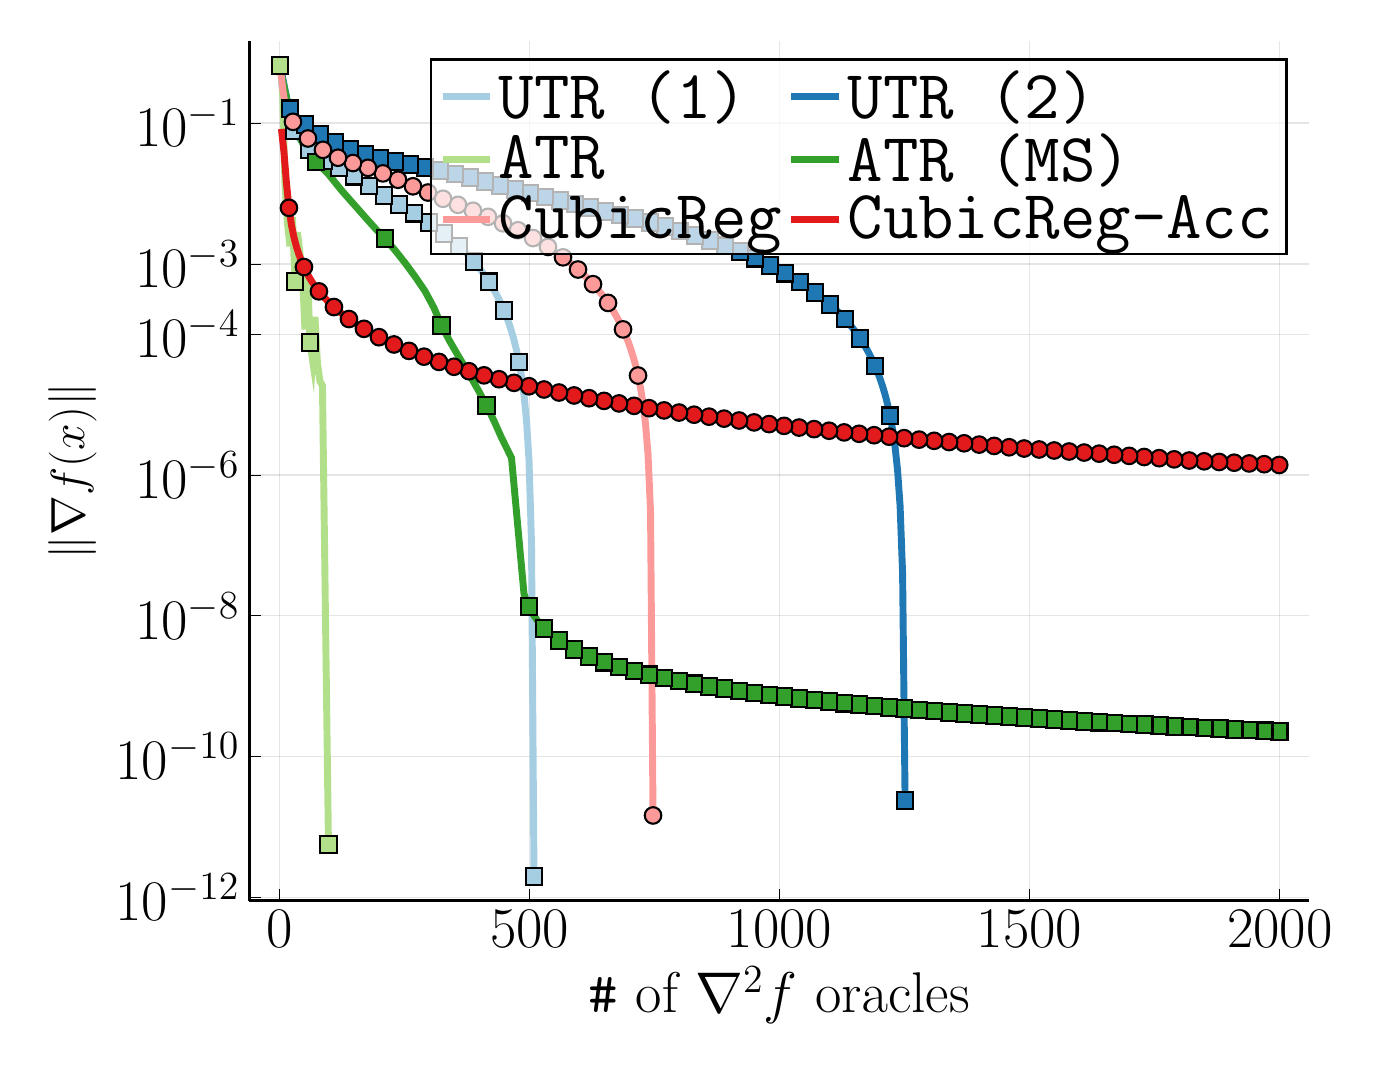
\begin{tikzpicture}[/tikz/background rectangle/.style={fill={rgb,1:red,1.0;green,1.0;blue,1.0}, fill opacity={1.0}, draw opacity={1.0}}, show background rectangle]
\begin{axis}[point meta max={nan}, point meta min={nan}, legend cell align={left}, legend columns={2}, title={}, title style={at={{(0.5,1)}}, anchor={south}, font={{\fontsize{22 pt}{28.6 pt}\selectfont}}, color={rgb,1:red,0.0;green,0.0;blue,0.0}, draw opacity={1.0}, rotate={0.0}, align={center}}, legend style={color={rgb,1:red,0.0;green,0.0;blue,0.0}, draw opacity={1.0}, line width={1}, solid, fill={rgb,1:red,1.0;green,1.0;blue,1.0}, fill opacity={0.7}, text opacity={1.0}, font={{\fontsize{24 pt}{31.200000000000003 pt}\selectfont}}, text={rgb,1:red,0.0;green,0.0;blue,0.0}, cells={anchor={west}}, at={(0.98, 0.98)}, anchor={north east}}, axis background/.style={fill={rgb,1:red,1.0;green,1.0;blue,1.0}, opacity={1.0}}, anchor={north west}, xshift={1.0mm}, yshift={-1.0mm}, width={150.4mm}, height={125.0mm}, scaled x ticks={false}, xlabel={\texttt{\#} of $\nabla^2f$ oracles}, x tick style={color={rgb,1:red,0.0;green,0.0;blue,0.0}, opacity={1.0}}, x tick label style={color={rgb,1:red,0.0;green,0.0;blue,0.0}, opacity={1.0}, rotate={0}}, xlabel style={at={(ticklabel cs:0.5)}, anchor=near ticklabel, at={{(ticklabel cs:0.5)}}, anchor={near ticklabel}, font={{\fontsize{20 pt}{26.0 pt}\selectfont}}, color={rgb,1:red,0.0;green,0.0;blue,0.0}, draw opacity={1.0}, rotate={0.0}}, xmajorgrids={true}, xmin={-59.97000000000003}, xmax={2058.9700000000003}, xticklabels={{$0$,$500$,$1000$,$1500$,$2000$}}, xtick={{0.0,500.0,1000.0,1500.0,2000.0}}, xtick align={inside}, xticklabel style={font={{\fontsize{20 pt}{26.0 pt}\selectfont}}, color={rgb,1:red,0.0;green,0.0;blue,0.0}, draw opacity={1.0}, rotate={0.0}}, x grid style={color={rgb,1:red,0.0;green,0.0;blue,0.0}, draw opacity={0.1}, line width={0.5}, solid}, axis x line*={left}, x axis line style={color={rgb,1:red,0.0;green,0.0;blue,0.0}, draw opacity={1.0}, line width={1}, solid}, scaled y ticks={false}, ylabel={$\|\nabla f(x)\|$}, y tick style={color={rgb,1:red,0.0;green,0.0;blue,0.0}, opacity={1.0}}, y tick label style={color={rgb,1:red,0.0;green,0.0;blue,0.0}, opacity={1.0}, rotate={0}}, ylabel style={at={(ticklabel cs:0.5)}, anchor=near ticklabel, at={{(ticklabel cs:0.5)}}, anchor={near ticklabel}, font={{\fontsize{17 pt}{22.1 pt}\selectfont}}, color={rgb,1:red,0.0;green,0.0;blue,0.0}, draw opacity={1.0}, rotate={0.0}}, ymode={log}, log basis y={10}, ymajorgrids={true}, ymin={8.939379885728391e-13}, ymax={1.4691333822015233}, yticklabels={{$10^{-12}$,$10^{-10}$,$10^{-8}$,$10^{-6}$,$10^{-4}$,$10^{-3}$,$10^{-1}$}}, ytick={{1.0e-12,1.0e-10,1.0e-8,1.0e-6,0.0001,0.001,0.1}}, ytick align={inside}, yticklabel style={font={{\fontsize{20 pt}{26.0 pt}\selectfont}}, color={rgb,1:red,0.0;green,0.0;blue,0.0}, draw opacity={1.0}, rotate={0.0}}, y grid style={color={rgb,1:red,0.0;green,0.0;blue,0.0}, draw opacity={0.1}, line width={0.5}, solid}, axis y line*={left}, y axis line style={color={rgb,1:red,0.0;green,0.0;blue,0.0}, draw opacity={1.0}, line width={1}, solid}, colorbar={false}]
    \addplot[color={rgb,1:red,0.651;green,0.808;blue,0.89}, name path={201}, draw opacity={1.0}, line width={2.5}, solid]
        table[row sep={\\}]
        {
            \\
            509.0  1.9816925442463838e-12  \\
            504.0  1.0835131551947725e-7  \\
            499.0  1.608248144722027e-6  \\
            494.0  5.926384264975321e-6  \\
            489.0  1.3645768992044188e-5  \\
            484.0  2.50441160049588e-5  \\
            479.0  4.029264782491237e-5  \\
            474.0  5.951486479663717e-5  \\
            469.0  8.280868883885579e-5  \\
            464.0  0.00011025666513324377  \\
            459.0  0.00014193162772297322  \\
            454.0  0.0001779005863779587  \\
            449.0  0.0002182280484124982  \\
            444.0  0.0002629793630946094  \\
            439.0  0.00031222434778245127  \\
            434.0  0.00036604121390522383  \\
            429.0  0.0004245205773937382  \\
            424.0  0.00048776908659721343  \\
            419.0  0.0005559119414355503  \\
            414.0  0.0006290933557639846  \\
            409.0  0.0007074739118196814  \\
            404.0  0.0007912238806046918  \\
            399.0  0.000880512047348733  \\
            394.0  0.0009754904536653023  \\
            389.0  0.0010762767034660481  \\
            384.0  0.0011829368583361687  \\
            379.0  0.001295473044413591  \\
            374.0  0.0014138201263694614  \\
            369.0  0.0015378546242538497  \\
            364.0  0.001667416276432185  \\
            359.0  0.0018023388657190187  \\
            354.0  0.0019424835645297082  \\
            349.0  0.002087766851782658  \\
            344.0  0.002238176905855765  \\
            339.0  0.00239377650603592  \\
            334.0  0.0025546948029517994  \\
            329.0  0.0027211128838731807  \\
            324.0  0.0028932482136512947  \\
            319.0  0.0030713414903027017  \\
            314.0  0.003255647453665088  \\
            309.0  0.0034464296592143003  \\
            304.0  0.0036439585085075283  \\
            299.0  0.003848511796887927  \\
            294.0  0.004060377425519651  \\
            289.0  0.0042798585044080345  \\
            284.0  0.004507281721452237  \\
            279.0  0.00474301047364664  \\
            274.0  0.004987464672504721  \\
            269.0  0.0052411490485760335  \\
            264.0  0.005504690878456762  \\
            259.0  0.00577888621153272  \\
            254.0  0.006064750982413885  \\
            249.0  0.006363569877033298  \\
            244.0  0.006676930946828065  \\
            239.0  0.007006726928446911  \\
            234.0  0.007355096165705075  \\
            229.0  0.007724274473901791  \\
            224.0  0.008116350672287461  \\
            219.0  0.008532975511004315  \\
            214.0  0.008975138440511088  \\
            209.0  0.00944311899404912  \\
            204.0  0.009936615529791899  \\
            199.0  0.010455036737556019  \\
            194.0  0.01099822777530089  \\
            189.0  0.011567996387253901  \\
            184.0  0.01216953724166414  \\
            179.0  0.012810609922216281  \\
            174.0  0.013498292549165772  \\
            169.0  0.014235848026799407  \\
            164.0  0.015022085370254977  \\
            159.0  0.015853164607991563  \\
            154.0  0.016723872288059886  \\
            149.0  0.01762612519701912  \\
            144.0  0.018549854840216557  \\
            139.0  0.019487969099118152  \\
            134.0  0.02043609396128469  \\
            129.0  0.021390378536925107  \\
            124.0  0.022347650217407252  \\
            119.0  0.023306384996017043  \\
            114.0  0.024268132916825936  \\
            109.0  0.025240004853930312  \\
            104.0  0.02623529856577574  \\
            99.0  0.027270346529396364  \\
            94.0  0.028370255428869572  \\
            89.0  0.029572758087033052  \\
            84.0  0.03092247965530352  \\
            79.0  0.03245444728154673  \\
            74.0  0.034211181585981555  \\
            69.0  0.036339852497757924  \\
            64.0  0.03898797734218703  \\
            59.0  0.042175274673628464  \\
            54.0  0.045826922726988614  \\
            49.0  0.05011178454052368  \\
            44.0  0.055220867166000394  \\
            39.0  0.06114243094368603  \\
            34.0  0.06872422835918174  \\
            29.0  0.07821227067981501  \\
            24.0  0.08939746014675029  \\
            19.0  0.1051753670769415  \\
            14.0  0.12653510891271635  \\
            9.0  0.16974630567632962  \\
            4.0  0.38902501645548354  \\
        }
        ;
    \addlegendentry {$\texttt{UTR (1)}$}
    \addplot[color={rgb,1:red,0.8889;green,0.4356;blue,0.2781}, name path={202}, only marks, draw opacity={1.0}, line width={0}, solid, mark={square*}, mark size={3.0 pt}, mark repeat={1}, mark options={color={rgb,1:red,0.0;green,0.0;blue,0.0}, draw opacity={1.0}, fill={rgb,1:red,0.651;green,0.808;blue,0.89}, fill opacity={1.0}, line width={0.75}, rotate={0}, solid}, forget plot]
        table[row sep={\\}]
        {
            \\
            509.0  1.9816925442463838e-12  \\
            479.0  4.029264782491237e-5  \\
            449.0  0.0002182280484124982  \\
            419.0  0.0005559119414355503  \\
            389.0  0.0010762767034660481  \\
            359.0  0.0018023388657190187  \\
            329.0  0.0027211128838731807  \\
            299.0  0.003848511796887927  \\
            269.0  0.0052411490485760335  \\
            239.0  0.007006726928446911  \\
            209.0  0.00944311899404912  \\
            179.0  0.012810609922216281  \\
            149.0  0.01762612519701912  \\
            119.0  0.023306384996017043  \\
            89.0  0.029572758087033052  \\
            59.0  0.042175274673628464  \\
            29.0  0.07821227067981501  \\
        }
        ;
    \addplot[color={rgb,1:red,0.122;green,0.471;blue,0.706}, name path={203}, draw opacity={1.0}, line width={2.5}, solid]
        table[row sep={\\}]
        {
            \\
            1251.0  2.3613012200513133e-11  \\
            1246.0  3.9867343092839975e-8  \\
            1241.0  3.6290584441244726e-7  \\
            1236.0  1.158186678014586e-6  \\
            1231.0  2.4980433356848835e-6  \\
            1226.0  4.417086544562135e-6  \\
            1221.0  6.9361254981605665e-6  \\
            1216.0  1.006961179732355e-5  \\
            1211.0  1.3828568455584939e-5  \\
            1206.0  1.8221955654616128e-5  \\
            1201.0  2.3257388780556168e-5  \\
            1196.0  2.89415507413282e-5  \\
            1191.0  3.528044529436206e-5  \\
            1186.0  4.227956135896567e-5  \\
            1181.0  4.994398459274133e-5  \\
            1176.0  5.827847637105644e-5  \\
            1171.0  6.728753201178717e-5  \\
            1166.0  7.697542556616931e-5  \\
            1161.0  8.734624590811107e-5  \\
            1156.0  9.840392730737641e-5  \\
            1151.0  0.00011015227671104035  \\
            1146.0  0.00012259499933777333  \\
            1141.0  0.00013573572377391577  \\
            1136.0  0.00014957802746905032  \\
            1131.0  0.00016412546331356993  \\
            1126.0  0.00017938158781139032  \\
            1121.0  0.00019534999121794474  \\
            1116.0  0.0002120343298837085  \\
            1111.0  0.00022943836091787493  \\
            1106.0  0.00024756597915900766  \\
            1101.0  0.00026642125630519026  \\
            1096.0  0.0002860084819123874  \\
            1091.0  0.00030633220581482333  \\
            1086.0  0.00032739728135457386  \\
            1081.0  0.0003492089086300922  \\
            1076.0  0.00037177267678710745  \\
            1071.0  0.0003950946041837994  \\
            1066.0  0.00041918117507063537  \\
            1061.0  0.0004440393712406076  \\
            1056.0  0.00046967669693678246  \\
            1051.0  0.0004961011951617285  \\
            1046.0  0.0005233214534299872  \\
            1041.0  0.0005513465969543379  \\
            1036.0  0.0005801862672743104  \\
            1031.0  0.0006098505844368883  \\
            1026.0  0.000640350091039694  \\
            1021.0  0.0006716956767602519  \\
            1016.0  0.0007038984824319872  \\
            1011.0  0.0007369697832954923  \\
            1006.0  0.0007709208517535716  \\
            1001.0  0.0008057628007843171  \\
            996.0  0.0008415064101035247  \\
            991.0  0.0008781619381909983  \\
            986.0  0.0009157389243694193  \\
            981.0  0.0009542459862022974  \\
            976.0  0.0009936906185014187  \\
            971.0  0.0010340790011364514  \\
            966.0  0.0010754158235443284  \\
            961.0  0.0011177041342640172  \\
            956.0  0.001160945223893418  \\
            951.0  0.0012051385495064242  \\
            946.0  0.001250281707720839  \\
            941.0  0.0012963704622365392  \\
            936.0  0.0013433988297664166  \\
            931.0  0.0013913592259010709  \\
            926.0  0.001440242669673649  \\
            921.0  0.001490039042568355  \\
            916.0  0.0015407373946404366  \\
            911.0  0.0015923262875213392  \\
            906.0  0.0016447941616237502  \\
            901.0  0.001698129713082664  \\
            896.0  0.0017523222650751968  \\
            891.0  0.0018073621182860301  \\
            886.0  0.0018632408664629842  \\
            881.0  0.0019199516651638132  \\
            876.0  0.001977489444750192  \\
            871.0  0.0020358510621706384  \\
            866.0  0.0020950353897710846  \\
            861.0  0.00215504334294971  \\
            856.0  0.0022158778516331683  \\
            851.0  0.0022775437830632106  \\
            846.0  0.002340047825104087  \\
            841.0  0.0024033983401666754  \\
            836.0  0.0024676051999388826  \\
            831.0  0.0025326796105276223  \\
            826.0  0.002598633936515672  \\
            821.0  0.0026654815309960925  \\
            816.0  0.002733236577043656  \\
            811.0  0.002801913944471177  \\
            806.0  0.0028715290642212093  \\
            801.0  0.002942097821445885  \\
            796.0  0.003013636467279436  \\
            791.0  0.003086161548527354  \\
            786.0  0.0031596898539763157  \\
            781.0  0.0032342383757456602  \\
            776.0  0.003309824284019208  \\
            771.0  0.003386464913576429  \\
            766.0  0.0034641777607460015  \\
            761.0  0.0035429804896981425  \\
            756.0  0.003622890947347611  \\
            751.0  0.0037039271865361434  \\
            746.0  0.0037861074975884174  \\
            741.0  0.0038694504487814508  \\
            736.0  0.003953974936729362  \\
            731.0  0.004039700248159658  \\
            726.0  0.004126646135037328  \\
            721.0  0.004214832905467039  \\
            716.0  0.004304281533252239  \\
            711.0  0.004395013789384293  \\
            706.0  0.004487052399037684  \\
            701.0  0.0045804212278145835  \\
            696.0  0.004675145500966184  \\
            691.0  0.004771252059073834  \\
            686.0  0.004868769653162363  \\
            681.0  0.0049677292814174386  \\
            676.0  0.005068164568582597  \\
            671.0  0.005170112187732963  \\
            666.0  0.005273612322491426  \\
            661.0  0.005378709165906602  \\
            656.0  0.005485451450183078  \\
            651.0  0.005593892999254823  \\
            646.0  0.005704093293796937  \\
            641.0  0.005816118035603839  \\
            636.0  0.005930039695195449  \\
            631.0  0.006045938022876937  \\
            626.0  0.006163900499089098  \\
            621.0  0.006284022694602653  \\
            616.0  0.006406408504903032  \\
            611.0  0.0065311702161724786  \\
            606.0  0.006658428353133564  \\
            601.0  0.006788311252681552  \\
            596.0  0.006920954303321408  \\
            591.0  0.007056498791249558  \\
            586.0  0.007195090302429762  \\
            581.0  0.007336876649482071  \\
            576.0  0.007482005325516714  \\
            571.0  0.007630620535464636  \\
            566.0  0.0077828599169820585  \\
            561.0  0.007938851130733338  \\
            556.0  0.008098708561208548  \\
            551.0  0.008262530407168076  \\
            546.0  0.008430396437798894  \\
            541.0  0.008602366635169506  \\
            536.0  0.008778480837179562  \\
            531.0  0.008958759357744647  \\
            526.0  0.009143204431175927  \\
            521.0  0.009331802258647255  \\
            516.0  0.009524525483657629  \\
            511.0  0.009721336135729267  \\
            506.0  0.009922189464622824  \\
            501.0  0.010127039574244363  \\
            496.0  0.010335848173988922  \\
            491.0  0.010548597777290806  \\
            486.0  0.010765309900337533  \\
            481.0  0.01098606701660358  \\
            476.0  0.01121103452970256  \\
            471.0  0.011440476947523455  \\
            466.0  0.011674762209370516  \\
            461.0  0.011914350383223657  \\
            456.0  0.012159766842221427  \\
            451.0  0.012411563748817038  \\
            446.0  0.012670275862028768  \\
            441.0  0.012936377151454783  \\
            436.0  0.01321024404561499  \\
            431.0  0.013492129951007771  \\
            426.0  0.013782154139160467  \\
            421.0  0.014080306102439596  \\
            416.0  0.014386463942308983  \\
            411.0  0.014700422486605476  \\
            406.0  0.015021924185007321  \\
            401.0  0.015350684086955654  \\
            396.0  0.015686399999242786  \\
            391.0  0.016028741202864995  \\
            386.0  0.01637731589049248  \\
            381.0  0.016731630710939263  \\
            376.0  0.017091071313389144  \\
            371.0  0.017454934109150024  \\
            366.0  0.01782251013223844  \\
            361.0  0.018193177919606725  \\
            356.0  0.018566451080345305  \\
            351.0  0.018941963993257756  \\
            346.0  0.01931942329010619  \\
            341.0  0.01969856262306721  \\
            336.0  0.0200791195549206  \\
            331.0  0.02046083258129627  \\
            326.0  0.020843447545546238  \\
            321.0  0.021226725550124077  \\
            316.0  0.021610451489785874  \\
            311.0  0.021994445414288088  \\
            306.0  0.022378576004391946  \\
            301.0  0.022762772952437407  \\
            296.0  0.023147039187882783  \\
            291.0  0.023531470520518866  \\
            286.0  0.023916289430943014  \\
            281.0  0.024301888821755043  \\
            276.0  0.024688867663324662  \\
            271.0  0.0250780323389438  \\
            266.0  0.025470343876134185  \\
            261.0  0.025866825001583757  \\
            256.0  0.026268498762974525  \\
            251.0  0.02667644945714469  \\
            246.0  0.02709200047896712  \\
            241.0  0.02751687016143421  \\
            236.0  0.027953183389357684  \\
            231.0  0.028403371444486812  \\
            226.0  0.028870085438228162  \\
            221.0  0.029356184305429325  \\
            216.0  0.029864709723144117  \\
            211.0  0.030398678195029626  \\
            206.0  0.030960624969719196  \\
            201.0  0.03155216430545887  \\
            196.0  0.032174274750794506  \\
            191.0  0.0328289179725519  \\
            186.0  0.03352124963488734  \\
            181.0  0.0342607337469342  \\
            176.0  0.03506060286372869  \\
            171.0  0.03593511581598159  \\
            166.0  0.03689387355271308  \\
            161.0  0.03793898940018324  \\
            156.0  0.0390710059601862  \\
            151.0  0.040293924895796474  \\
            146.0  0.04160354337424029  \\
            141.0  0.0429789469264583  \\
            136.0  0.04442346741649353  \\
            131.0  0.04595988430608248  \\
            126.0  0.04759405742915778  \\
            121.0  0.04934441678978815  \\
            116.0  0.051235170968708665  \\
            111.0  0.05326914963488664  \\
            106.0  0.05543924270453537  \\
            101.0  0.057729458712066306  \\
            96.0  0.060141490794564975  \\
            91.0  0.0627988635431057  \\
            86.0  0.06581978196151053  \\
            81.0  0.06917229838275969  \\
            76.0  0.07284927862261623  \\
            71.0  0.0767829395013382  \\
            66.0  0.08088091893901245  \\
            61.0  0.08535165710141257  \\
            56.0  0.09026179466852476  \\
            51.0  0.09618956858547958  \\
            46.0  0.10305123505308605  \\
            41.0  0.11077765988945863  \\
            36.0  0.11954132960580181  \\
            31.0  0.12864869102540402  \\
            26.0  0.13986184776972987  \\
            21.0  0.15965489937413702  \\
            16.0  0.20412054817792644  \\
            11.0  0.29949070737706207  \\
            6.0  0.458525397878602  \\
            1.0  0.6627234605304922  \\
        }
        ;
    \addlegendentry {$\texttt{UTR (2)}$}
    \addplot[color={rgb,1:red,0.7644;green,0.4441;blue,0.8243}, name path={204}, only marks, draw opacity={1.0}, line width={0}, solid, mark={square*}, mark size={3.0 pt}, mark repeat={1}, mark options={color={rgb,1:red,0.0;green,0.0;blue,0.0}, draw opacity={1.0}, fill={rgb,1:red,0.122;green,0.471;blue,0.706}, fill opacity={1.0}, line width={0.75}, rotate={0}, solid}, forget plot]
        table[row sep={\\}]
        {
            \\
            1251.0  2.3613012200513133e-11  \\
            1221.0  6.9361254981605665e-6  \\
            1191.0  3.528044529436206e-5  \\
            1161.0  8.734624590811107e-5  \\
            1131.0  0.00016412546331356993  \\
            1101.0  0.00026642125630519026  \\
            1071.0  0.0003950946041837994  \\
            1041.0  0.0005513465969543379  \\
            1011.0  0.0007369697832954923  \\
            981.0  0.0009542459862022974  \\
            951.0  0.0012051385495064242  \\
            921.0  0.001490039042568355  \\
            891.0  0.0018073621182860301  \\
            861.0  0.00215504334294971  \\
            831.0  0.0025326796105276223  \\
            801.0  0.002942097821445885  \\
            771.0  0.003386464913576429  \\
            741.0  0.0038694504487814508  \\
            711.0  0.004395013789384293  \\
            681.0  0.0049677292814174386  \\
            651.0  0.005593892999254823  \\
            621.0  0.006284022694602653  \\
            591.0  0.007056498791249558  \\
            561.0  0.007938851130733338  \\
            531.0  0.008958759357744647  \\
            501.0  0.010127039574244363  \\
            471.0  0.011440476947523455  \\
            441.0  0.012936377151454783  \\
            411.0  0.014700422486605476  \\
            381.0  0.016731630710939263  \\
            351.0  0.018941963993257756  \\
            321.0  0.021226725550124077  \\
            291.0  0.023531470520518866  \\
            261.0  0.025866825001583757  \\
            231.0  0.028403371444486812  \\
            201.0  0.03155216430545887  \\
            171.0  0.03593511581598159  \\
            141.0  0.0429789469264583  \\
            111.0  0.05326914963488664  \\
            81.0  0.06917229838275969  \\
            51.0  0.09618956858547958  \\
            21.0  0.15965489937413702  \\
        }
        ;
    \addplot[color={rgb,1:red,0.698;green,0.875;blue,0.541}, name path={205}, draw opacity={1.0}, line width={2.5}, solid]
        table[row sep={\\}]
        {
            \\
            98.0  5.593287293545348e-12  \\
            86.0  1.8559519083601965e-5  \\
            81.0  2.1445336068602816e-5  \\
            76.0  3.860326856664707e-5  \\
            71.0  0.00017695976585330173  \\
            66.0  4.3861947566294376e-5  \\
            61.0  7.651044805383612e-5  \\
            56.0  0.0008965110529427119  \\
            51.0  0.00011663840262948298  \\
            46.0  0.0007340958461590139  \\
            41.0  0.0014250206926127642  \\
            36.0  0.002818922941335248  \\
            31.0  0.0005660586701902481  \\
            26.0  0.004609550986646257  \\
            21.0  0.001777099428032272  \\
            16.0  0.0037955825508568927  \\
            11.0  0.014200192148289345  \\
            6.0  0.3505887388550164  \\
            1.0  0.6627234605304922  \\
        }
        ;
    \addlegendentry {$\texttt{ATR}$}
    \addplot[color={rgb,1:red,0.0;green,0.6658;blue,0.681}, name path={206}, only marks, draw opacity={1.0}, line width={0}, solid, mark={square*}, mark size={3.0 pt}, mark repeat={1}, mark options={color={rgb,1:red,0.0;green,0.0;blue,0.0}, draw opacity={1.0}, fill={rgb,1:red,0.698;green,0.875;blue,0.541}, fill opacity={1.0}, line width={0.75}, rotate={0}, solid}, forget plot]
        table[row sep={\\}]
        {
            \\
            98.0  5.593287293545348e-12  \\
            61.0  7.651044805383612e-5  \\
            31.0  0.0005660586701902481  \\
            1.0  0.6627234605304922  \\
        }
        ;
    \addplot[color={rgb,1:red,0.2;green,0.627;blue,0.173}, name path={207}, draw opacity={1.0}, line width={2.5}, solid]
        table[row sep={\\}]
        {
            \\
            1999.0  2.2683345637621003e-10  \\
            1994.0  2.2768750083346558e-10  \\
            1989.0  2.2854722957861232e-10  \\
            1984.0  2.2941261822499192e-10  \\
            1979.0  2.3028397233818602e-10  \\
            1974.0  2.3116232934075966e-10  \\
            1969.0  2.3204497054596662e-10  \\
            1964.0  2.3293348990449344e-10  \\
            1959.0  2.3382860347420135e-10  \\
            1954.0  2.3472810577324224e-10  \\
            1949.0  2.356362232311293e-10  \\
            1944.0  2.3655040893573287e-10  \\
            1939.0  2.37469032375425e-10  \\
            1934.0  2.3839611966861295e-10  \\
            1929.0  2.393285694645529e-10  \\
            1924.0  2.402674277828558e-10  \\
            1919.0  2.4121266156472995e-10  \\
            1914.0  2.4216425812908193e-10  \\
            1909.0  2.431236103315928e-10  \\
            1904.0  2.4409049063790395e-10  \\
            1899.0  2.450633792667382e-10  \\
            1894.0  2.460436191831087e-10  \\
            1889.0  2.470292291695902e-10  \\
            1884.0  2.4802154069809786e-10  \\
            1879.0  2.490219763030864e-10  \\
            1874.0  2.500293100936375e-10  \\
            1869.0  2.510452756402831e-10  \\
            1864.0  2.520664935320844e-10  \\
            1859.0  2.530966388908948e-10  \\
            1854.0  2.5413225531826456e-10  \\
            1849.0  2.551766775859088e-10  \\
            1844.0  2.562275809467251e-10  \\
            1839.0  2.572872713512518e-10  \\
            1834.0  2.5835550798334616e-10  \\
            1829.0  2.5943067716357186e-10  \\
            1824.0  2.605141834403903e-10  \\
            1819.0  2.616059564656352e-10  \\
            1814.0  2.627045398910865e-10  \\
            1809.0  2.6381355528096493e-10  \\
            1804.0  2.6492832692137964e-10  \\
            1799.0  2.6605302089303457e-10  \\
            1794.0  2.6718675734199027e-10  \\
            1789.0  2.683292631759646e-10  \\
            1784.0  2.694797783849083e-10  \\
            1779.0  2.706386948437619e-10  \\
            1774.0  2.718078088828966e-10  \\
            1769.0  2.7298638730275883e-10  \\
            1764.0  2.741716560610123e-10  \\
            1759.0  2.7536574434407687e-10  \\
            1754.0  2.7657123761260145e-10  \\
            1749.0  2.7778754205203744e-10  \\
            1744.0  2.7901164142602853e-10  \\
            1739.0  2.802448306703934e-10  \\
            1734.0  2.8148990026338314e-10  \\
            1729.0  2.827430203062272e-10  \\
            1724.0  2.840076816141973e-10  \\
            1719.0  2.8528084442307886e-10  \\
            1714.0  2.8656460646351916e-10  \\
            1709.0  2.8785891923175257e-10  \\
            1704.0  2.891638324403565e-10  \\
            1699.0  2.904811188400979e-10  \\
            1694.0  2.9180684664726914e-10  \\
            1689.0  2.9314366374587557e-10  \\
            1684.0  2.9449298407314665e-10  \\
            1679.0  2.9585192918278286e-10  \\
            1674.0  2.9722307009591434e-10  \\
            1669.0  2.986050146549235e-10  \\
            1664.0  2.9999799848106895e-10  \\
            1659.0  3.0140409748047323e-10  \\
            1654.0  3.0282251504237143e-10  \\
            1649.0  3.0425227828780973e-10  \\
            1644.0  3.0569505005027595e-10  \\
            1639.0  3.071496916021656e-10  \\
            1634.0  3.086175376535785e-10  \\
            1629.0  3.100983347772279e-10  \\
            1624.0  3.115905386164571e-10  \\
            1619.0  3.1309550386479984e-10  \\
            1614.0  3.1461300909964056e-10  \\
            1609.0  3.1614445771161297e-10  \\
            1604.0  3.1768905219701003e-10  \\
            1599.0  3.1924931224182757e-10  \\
            1594.0  3.2082273998572983e-10  \\
            1589.0  3.2241132904625575e-10  \\
            1584.0  3.24013587409876e-10  \\
            1579.0  3.2563068686531166e-10  \\
            1574.0  3.272601738925512e-10  \\
            1569.0  3.289067374938808e-10  \\
            1564.0  3.30567646739557e-10  \\
            1559.0  3.322426403714561e-10  \\
            1554.0  3.3393490442575864e-10  \\
            1549.0  3.356424162643819e-10  \\
            1544.0  3.373650677589393e-10  \\
            1539.0  3.3910497610836725e-10  \\
            1534.0  3.408614899723109e-10  \\
            1529.0  3.426330663635074e-10  \\
            1524.0  3.444218958846286e-10  \\
            1519.0  3.462290946852827e-10  \\
            1514.0  3.480536783309649e-10  \\
            1509.0  3.4989618397548983e-10  \\
            1504.0  3.517567555120499e-10  \\
            1499.0  3.5363419663679214e-10  \\
            1494.0  3.5552978056116456e-10  \\
            1489.0  3.574422688431479e-10  \\
            1484.0  3.593748747394047e-10  \\
            1479.0  3.6132848232042306e-10  \\
            1474.0  3.6330059522098625e-10  \\
            1469.0  3.6529337008354504e-10  \\
            1464.0  3.673055280523259e-10  \\
            1459.0  3.6933825351106406e-10  \\
            1454.0  3.71390950703535e-10  \\
            1449.0  3.7346503086188683e-10  \\
            1444.0  3.7556124924488e-10  \\
            1439.0  3.77677477027827e-10  \\
            1434.0  3.7981747653704717e-10  \\
            1429.0  3.8197825122536025e-10  \\
            1424.0  3.841624700242377e-10  \\
            1419.0  3.863706308405723e-10  \\
            1414.0  3.886013388910894e-10  \\
            1409.0  3.9085576645699173e-10  \\
            1404.0  3.931340182781745e-10  \\
            1399.0  3.954378781845999e-10  \\
            1394.0  3.9776754940265975e-10  \\
            1389.0  4.001203269803696e-10  \\
            1384.0  4.024995246065243e-10  \\
            1379.0  4.0490581113771497e-10  \\
            1374.0  4.0733797194009067e-10  \\
            1369.0  4.0979630173552365e-10  \\
            1364.0  4.1228303615139356e-10  \\
            1359.0  4.1479840090565075e-10  \\
            1354.0  4.1734159789707374e-10  \\
            1349.0  4.1991297257866814e-10  \\
            1344.0  4.225138642080036e-10  \\
            1339.0  4.251454435759988e-10  \\
            1334.0  4.2780692194263447e-10  \\
            1329.0  4.3049983567583314e-10  \\
            1324.0  4.3322375368921063e-10  \\
            1319.0  4.359815998568388e-10  \\
            1314.0  4.3877319691422885e-10  \\
            1309.0  4.4159608449852324e-10  \\
            1304.0  4.4445383096909756e-10  \\
            1299.0  4.4734583278962985e-10  \\
            1294.0  4.5027160676564985e-10  \\
            1289.0  4.5323308384423625e-10  \\
            1284.0  4.562328483070422e-10  \\
            1279.0  4.5926734433350974e-10  \\
            1274.0  4.6234049751288134e-10  \\
            1269.0  4.6545218731869685e-10  \\
            1264.0  4.686032876143072e-10  \\
            1259.0  4.717953214216475e-10  \\
            1254.0  4.750276557820805e-10  \\
            1249.0  4.782995980366629e-10  \\
            1244.0  4.816151322618309e-10  \\
            1239.0  4.849743835263978e-10  \\
            1234.0  4.883775302451562e-10  \\
            1229.0  4.918252336758819e-10  \\
            1224.0  4.953189767367358e-10  \\
            1219.0  4.988608451088245e-10  \\
            1214.0  5.024485035973612e-10  \\
            1209.0  5.060855431799791e-10  \\
            1204.0  5.097712617955573e-10  \\
            1199.0  5.135062429453429e-10  \\
            1194.0  5.17293652615682e-10  \\
            1189.0  5.211338268015909e-10  \\
            1184.0  5.250275351516368e-10  \\
            1179.0  5.289765321091336e-10  \\
            1174.0  5.329813105552366e-10  \\
            1169.0  5.370433985886197e-10  \\
            1164.0  5.411642347998435e-10  \\
            1159.0  5.453445211280294e-10  \\
            1154.0  5.495872422876941e-10  \\
            1149.0  5.538899623872138e-10  \\
            1144.0  5.582581417121505e-10  \\
            1139.0  5.626923654281822e-10  \\
            1134.0  5.671919136875537e-10  \\
            1129.0  5.717602114763704e-10  \\
            1124.0  5.763986278953065e-10  \\
            1119.0  5.811075944926008e-10  \\
            1114.0  5.858892748562058e-10  \\
            1109.0  5.90745614335784e-10  \\
            1104.0  5.956813010390592e-10  \\
            1099.0  6.00693714602507e-10  \\
            1094.0  6.057861909590353e-10  \\
            1089.0  6.109614446146055e-10  \\
            1084.0  6.162203442274458e-10  \\
            1079.0  6.215667267744877e-10  \\
            1074.0  6.270002946770014e-10  \\
            1069.0  6.325226207495495e-10  \\
            1064.0  6.381394027339883e-10  \\
            1059.0  6.438513645114462e-10  \\
            1054.0  6.496604854558709e-10  \\
            1049.0  6.555685752373839e-10  \\
            1044.0  6.615810043090231e-10  \\
            1039.0  6.676999976525597e-10  \\
            1034.0  6.739257657078243e-10  \\
            1029.0  6.802625560163758e-10  \\
            1024.0  6.867141746074397e-10  \\
            1019.0  6.932825535826457e-10  \\
            1014.0  6.999722217167579e-10  \\
            1009.0  7.067839935875982e-10  \\
            1004.0  7.137240198284206e-10  \\
            999.0  7.207957875655847e-10  \\
            994.0  7.280012894034006e-10  \\
            989.0  7.353460130086192e-10  \\
            984.0  7.428341810237004e-10  \\
            979.0  7.504680165086677e-10  \\
            974.0  7.582526707817279e-10  \\
            969.0  7.66193301845002e-10  \\
            964.0  7.742953225785476e-10  \\
            959.0  7.82561624403882e-10  \\
            954.0  7.909976869874902e-10  \\
            949.0  7.996096077110675e-10  \\
            944.0  8.084032825811885e-10  \\
            939.0  8.173832823936233e-10  \\
            934.0  8.265574286480147e-10  \\
            929.0  8.359310611754131e-10  \\
            924.0  8.455109040822083e-10  \\
            919.0  8.553045157605725e-10  \\
            914.0  8.653163517723274e-10  \\
            909.0  8.755566902173833e-10  \\
            904.0  8.86031608822263e-10  \\
            899.0  8.967498215585991e-10  \\
            894.0  9.077201137307461e-10  \\
            889.0  9.189507904602132e-10  \\
            884.0  9.304525553026139e-10  \\
            879.0  9.42235043011372e-10  \\
            874.0  9.543088027581546e-10  \\
            869.0  9.666838935743198e-10  \\
            864.0  9.793706993333765e-10  \\
            859.0  9.923837130606578e-10  \\
            854.0  1.005733417216313e-9  \\
            849.0  1.0194356069197976e-9  \\
            844.0  1.0335022570057643e-9  \\
            839.0  1.0479475392211171e-9  \\
            834.0  1.0627889746326506e-9  \\
            829.0  1.0780417293677937e-9  \\
            824.0  1.093724364402153e-9  \\
            819.0  1.1098542451160777e-9  \\
            814.0  1.1264528822515982e-9  \\
            809.0  1.1435388121866243e-9  \\
            804.0  1.1611339205652073e-9  \\
            799.0  1.1792621758573506e-9  \\
            794.0  1.1979479404645938e-9  \\
            789.0  1.2172165038666216e-9  \\
            784.0  1.237096282452985e-9  \\
            779.0  1.257617174133032e-9  \\
            774.0  1.2788098650513669e-9  \\
            769.0  1.3007069377922677e-9  \\
            764.0  1.323347127615856e-9  \\
            759.0  1.3467669117619666e-9  \\
            754.0  1.371008356115192e-9  \\
            749.0  1.3961144701211622e-9  \\
            744.0  1.422132804935644e-9  \\
            739.0  1.4491142277028487e-9  \\
            734.0  1.47711215900824e-9  \\
            729.0  1.5061863955295037e-9  \\
            724.0  1.536398914952566e-9  \\
            719.0  1.567819849113597e-9  \\
            714.0  1.600522271078934e-9  \\
            709.0  1.634585584753831e-9  \\
            704.0  1.6700981810710444e-9  \\
            699.0  1.7071532444986147e-9  \\
            694.0  1.7458533297819753e-9  \\
            689.0  1.786311719611097e-9  \\
            684.0  1.8286501316203273e-9  \\
            679.0  1.8730029649512298e-9  \\
            674.0  1.919518404074753e-9  \\
            669.0  1.968357979168362e-9  \\
            664.0  2.019700829554997e-9  \\
            659.0  2.0737438465718814e-9  \\
            654.0  2.1307056473136663e-9  \\
            649.0  2.190831562397144e-9  \\
            644.0  2.2543919499038017e-9  \\
            639.0  2.3216888995119003e-9  \\
            634.0  2.393063798501887e-9  \\
            629.0  2.4688985855988575e-9  \\
            624.0  2.5496251097279e-9  \\
            619.0  2.6357336824341057e-9  \\
            614.0  2.7277814068623134e-9  \\
            609.0  2.8264048074785316e-9  \\
            604.0  2.932336639530054e-9  \\
            599.0  3.046421815014156e-9  \\
            594.0  3.1696393017107617e-9  \\
            589.0  3.303134574218688e-9  \\
            584.0  3.4482507462778694e-9  \\
            579.0  3.6065761250631893e-9  \\
            574.0  3.7800058491769396e-9  \\
            569.0  3.970812027569391e-9  \\
            564.0  4.181749155955472e-9  \\
            559.0  4.4161873298762126e-9  \\
            554.0  4.678296188106402e-9  \\
            549.0  4.973292233516897e-9  \\
            544.0  5.307796124047155e-9  \\
            539.0  5.690336219526252e-9  \\
            534.0  6.132094691682917e-9  \\
            529.0  6.6480224715219755e-9  \\
            524.0  7.258581497794335e-9  \\
            519.0  7.992547580015608e-9  \\
            514.0  8.89172408999644e-9  \\
            509.0  1.0019388404929525e-8  \\
            504.0  1.147646077570551e-8  \\
            499.0  1.3432538019079424e-8  \\
            494.0  1.6199384855980793e-8  \\
            489.0  2.0419690096927195e-8  \\
            464.0  1.7555668678028936e-6  \\
            444.0  3.3861314060582965e-6  \\
            429.0  5.8788530064915634e-6  \\
            414.0  9.691123136292884e-6  \\
            399.0  1.537903658852036e-5  \\
            384.0  2.3740703579209467e-5  \\
            369.0  3.6012695519174176e-5  \\
            354.0  5.436417780139757e-5  \\
            339.0  8.326607088253042e-5  \\
            324.0  0.0001336554744120946  \\
            309.0  0.00023690842197635677  \\
            291.0  0.0004105342358533998  \\
            271.0  0.0006637901600346606  \\
            251.0  0.0010348172378571822  \\
            231.0  0.0015667992850256658  \\
            211.0  0.002281385356539828  \\
            191.0  0.003221959560367883  \\
            171.0  0.004647682276305379  \\
            148.0  0.007116065685005835  \\
            123.0  0.011312349647863833  \\
            98.0  0.018807878673589584  \\
            73.0  0.028101106708246535  \\
            48.0  0.04892486244964463  \\
            23.0  0.11579628058572482  \\
            0.0  0.6627234605304922  \\
        }
        ;
    \addlegendentry {$\texttt{ATR (MS)}$}
    \addplot[color={rgb,1:red,0.777;green,0.5097;blue,0.1464}, name path={208}, only marks, draw opacity={1.0}, line width={0}, solid, mark={square*}, mark size={3.0 pt}, mark repeat={1}, mark options={color={rgb,1:red,0.0;green,0.0;blue,0.0}, draw opacity={1.0}, fill={rgb,1:red,0.2;green,0.627;blue,0.173}, fill opacity={1.0}, line width={0.75}, rotate={0}, solid}, forget plot]
        table[row sep={\\}]
        {
            \\
            1999.0  2.2683345637621003e-10  \\
            1969.0  2.3204497054596662e-10  \\
            1939.0  2.37469032375425e-10  \\
            1909.0  2.431236103315928e-10  \\
            1879.0  2.490219763030864e-10  \\
            1849.0  2.551766775859088e-10  \\
            1819.0  2.616059564656352e-10  \\
            1789.0  2.683292631759646e-10  \\
            1759.0  2.7536574434407687e-10  \\
            1729.0  2.827430203062272e-10  \\
            1699.0  2.904811188400979e-10  \\
            1669.0  2.986050146549235e-10  \\
            1639.0  3.071496916021656e-10  \\
            1609.0  3.1614445771161297e-10  \\
            1579.0  3.2563068686531166e-10  \\
            1549.0  3.356424162643819e-10  \\
            1519.0  3.462290946852827e-10  \\
            1489.0  3.574422688431479e-10  \\
            1459.0  3.6933825351106406e-10  \\
            1429.0  3.8197825122536025e-10  \\
            1399.0  3.954378781845999e-10  \\
            1369.0  4.0979630173552365e-10  \\
            1339.0  4.251454435759988e-10  \\
            1309.0  4.4159608449852324e-10  \\
            1279.0  4.5926734433350974e-10  \\
            1249.0  4.782995980366629e-10  \\
            1219.0  4.988608451088245e-10  \\
            1189.0  5.211338268015909e-10  \\
            1159.0  5.453445211280294e-10  \\
            1129.0  5.717602114763704e-10  \\
            1099.0  6.00693714602507e-10  \\
            1069.0  6.325226207495495e-10  \\
            1039.0  6.676999976525597e-10  \\
            1009.0  7.067839935875982e-10  \\
            979.0  7.504680165086677e-10  \\
            949.0  7.996096077110675e-10  \\
            919.0  8.553045157605725e-10  \\
            889.0  9.189507904602132e-10  \\
            859.0  9.923837130606578e-10  \\
            829.0  1.0780417293677937e-9  \\
            799.0  1.1792621758573506e-9  \\
            769.0  1.3007069377922677e-9  \\
            739.0  1.4491142277028487e-9  \\
            709.0  1.634585584753831e-9  \\
            679.0  1.8730029649512298e-9  \\
            649.0  2.190831562397144e-9  \\
            619.0  2.6357336824341057e-9  \\
            589.0  3.303134574218688e-9  \\
            559.0  4.4161873298762126e-9  \\
            529.0  6.6480224715219755e-9  \\
            499.0  1.3432538019079424e-8  \\
            414.0  9.691123136292884e-6  \\
            324.0  0.0001336554744120946  \\
            211.0  0.002281385356539828  \\
            73.0  0.028101106708246535  \\
        }
        ;
    \addplot[color={rgb,1:red,0.984;green,0.604;blue,0.6}, name path={209}, draw opacity={1.0}, line width={2.5}, solid]
        table[row sep={\\}]
        {
            \\
            747.0  1.4538775997591908e-11  \\
            742.0  2.996807125645809e-7  \\
            737.0  1.9639067179086254e-6  \\
            732.0  5.2974611408871516e-6  \\
            727.0  1.0372079028333707e-5  \\
            722.0  1.722918672673381e-5  \\
            717.0  2.5900592555362626e-5  \\
            712.0  3.641201168332213e-5  \\
            707.0  4.878530809461924e-5  \\
            702.0  6.304069059496745e-5  \\
            697.0  7.919663282332988e-5  \\
            692.0  9.726999009091737e-5  \\
            687.0  0.00011727672274877991  \\
            682.0  0.0001392330347140876  \\
            677.0  0.00016315576050069498  \\
            672.0  0.00018905916923840684  \\
            667.0  0.0002169624311643802  \\
            662.0  0.00024687982577119484  \\
            657.0  0.00027882891167069993  \\
            652.0  0.0003128337048524044  \\
            647.0  0.00034891303280882837  \\
            642.0  0.00038709310415130615  \\
            637.0  0.00042740172702723095  \\
            632.0  0.000469872098569493  \\
            627.0  0.0005145399028258564  \\
            622.0  0.0005614469309392368  \\
            617.0  0.0006106362294305533  \\
            612.0  0.0006621575713544619  \\
            607.0  0.0007160607432830245  \\
            602.0  0.0007723988193478991  \\
            597.0  0.0008312215311198589  \\
            592.0  0.00089258023323466  \\
            587.0  0.0009565156387297026  \\
            582.0  0.0010230644569404184  \\
            577.0  0.0010922545409127514  \\
            572.0  0.0011640963150791243  \\
            567.0  0.0012385892760116062  \\
            562.0  0.0013157189525812487  \\
            557.0  0.001395457449918635  \\
            552.0  0.0014777662829656617  \\
            547.0  0.001562593302015891  \\
            542.0  0.0016498864998771027  \\
            537.0  0.0017395941204926342  \\
            532.0  0.0018316683950943791  \\
            527.0  0.001926070154032426  \\
            522.0  0.0020227738029505605  \\
            517.0  0.0021217699274566114  \\
            512.0  0.002223062896143329  \\
            507.0  0.0023266733040853862  \\
            502.0  0.0024326332508458125  \\
            497.0  0.0025409945244612596  \\
            492.0  0.0026518095432473765  \\
            487.0  0.0027651425108825073  \\
            482.0  0.0028810641668604716  \\
            477.0  0.0029996489510288856  \\
            472.0  0.003120968862557002  \\
            467.0  0.003245106167293424  \\
            462.0  0.003372138299306611  \\
            457.0  0.0035021487008967947  \\
            452.0  0.0036352156815785117  \\
            447.0  0.0037714276418261182  \\
            442.0  0.00391086860329366  \\
            437.0  0.004053627614876343  \\
            432.0  0.004199793416916204  \\
            427.0  0.004349465818488446  \\
            422.0  0.004502745055527009  \\
            417.0  0.00465974158405741  \\
            412.0  0.004820578110060893  \\
            407.0  0.004985391196754293  \\
            402.0  0.005154336244593278  \\
            397.0  0.005327592306360621  \\
            392.0  0.005505369269355445  \\
            387.0  0.005687914423197763  \\
            382.0  0.005875526560707959  \\
            377.0  0.006068544609938113  \\
            372.0  0.006267371206082273  \\
            367.0  0.006472474255011667  \\
            362.0  0.006684382243232468  \\
            357.0  0.0069036830197156465  \\
            352.0  0.007131021827673671  \\
            347.0  0.007367076845922314  \\
            342.0  0.007612526987843453  \\
            337.0  0.007868024097587292  \\
            332.0  0.008134148291981544  \\
            327.0  0.008411358554241388  \\
            322.0  0.008699980783578306  \\
            317.0  0.009000186632631538  \\
            312.0  0.009312001560544158  \\
            307.0  0.009635337582519695  \\
            302.0  0.009970015978770274  \\
            297.0  0.010315836581798129  \\
            292.0  0.010672683306173303  \\
            287.0  0.011040738250422847  \\
            282.0  0.011420747747871402  \\
            277.0  0.011814208383508617  \\
            272.0  0.01222330957072724  \\
            267.0  0.012650554257105408  \\
            262.0  0.01309823810852688  \\
            257.0  0.013567941090466017  \\
            252.0  0.014060269602320536  \\
            247.0  0.014574883709132163  \\
            242.0  0.015110783933623868  \\
            237.0  0.015666670039578733  \\
            232.0  0.016241028399542792  \\
            227.0  0.016831870880732437  \\
            222.0  0.017436390600245343  \\
            217.0  0.018051354849791198  \\
            212.0  0.018674087194777096  \\
            207.0  0.019302832578579142  \\
            202.0  0.019936302596676652  \\
            197.0  0.020573286580395447  \\
            192.0  0.021212624093433125  \\
            187.0  0.021853304131497817  \\
            182.0  0.022494597307016077  \\
            177.0  0.023136211681541122  \\
            172.0  0.023778497788017203  \\
            167.0  0.024422807082181277  \\
            162.0  0.02507193920113921  \\
            157.0  0.02573005534735018  \\
            152.0  0.026401835600107827  \\
            147.0  0.027092475468739  \\
            142.0  0.02780940052436653  \\
            137.0  0.028562964347601912  \\
            132.0  0.029365536444923485  \\
            127.0  0.030230921327564123  \\
            122.0  0.03117213742369638  \\
            117.0  0.03219707465421923  \\
            112.0  0.03331501871177709  \\
            107.0  0.0345578892900978  \\
            102.0  0.03598497642128784  \\
            97.0  0.037645830879256104  \\
            92.0  0.0395503730553255  \\
            87.0  0.04170316220938293  \\
            82.0  0.044050656501530235  \\
            77.0  0.046639082805204554  \\
            72.0  0.0495268877494028  \\
            67.0  0.052797053641324074  \\
            62.0  0.05645127806654487  \\
            57.0  0.06045123449091596  \\
            52.0  0.06517715472109953  \\
            47.0  0.07086459217770755  \\
            42.0  0.07737598962279862  \\
            37.0  0.08452875557213371  \\
            32.0  0.09302709142190914  \\
            27.0  0.10427412703165066  \\
            22.0  0.11821450483320253  \\
            17.0  0.13435732766399158  \\
            12.0  0.16808903941232095  \\
            7.0  0.29422597798474015  \\
            2.0  0.5909332263672181  \\
        }
        ;
    \addlegendentry {$\texttt{CubicReg}$}
    \addplot[color={rgb,1:red,0.5585;green,0.5935;blue,0.1175}, name path={210}, only marks, draw opacity={1.0}, line width={0}, solid, mark={*}, mark size={3.0 pt}, mark repeat={1}, mark options={color={rgb,1:red,0.0;green,0.0;blue,0.0}, draw opacity={1.0}, fill={rgb,1:red,0.984;green,0.604;blue,0.6}, fill opacity={1.0}, line width={0.75}, rotate={0}, solid}, forget plot]
        table[row sep={\\}]
        {
            \\
            747.0  1.4538775997591908e-11  \\
            717.0  2.5900592555362626e-5  \\
            687.0  0.00011727672274877991  \\
            657.0  0.00027882891167069993  \\
            627.0  0.0005145399028258564  \\
            597.0  0.0008312215311198589  \\
            567.0  0.0012385892760116062  \\
            537.0  0.0017395941204926342  \\
            507.0  0.0023266733040853862  \\
            477.0  0.0029996489510288856  \\
            447.0  0.0037714276418261182  \\
            417.0  0.00465974158405741  \\
            387.0  0.005687914423197763  \\
            357.0  0.0069036830197156465  \\
            327.0  0.008411358554241388  \\
            297.0  0.010315836581798129  \\
            267.0  0.012650554257105408  \\
            237.0  0.015666670039578733  \\
            207.0  0.019302832578579142  \\
            177.0  0.023136211681541122  \\
            147.0  0.027092475468739  \\
            117.0  0.03219707465421923  \\
            87.0  0.04170316220938293  \\
            57.0  0.06045123449091596  \\
            27.0  0.10427412703165066  \\
        }
        ;
    \addplot[color={rgb,1:red,0.89;green,0.102;blue,0.11}, name path={211}, draw opacity={1.0}, line width={2.5}, solid]
        table[row sep={\\}]
        {
            \\
            1999.0  1.388358425888818e-6  \\
            1994.0  1.394325643927792e-6  \\
            1989.0  1.400294122955305e-6  \\
            1984.0  1.406263269203162e-6  \\
            1979.0  1.412232485984153e-6  \\
            1974.0  1.4182011549297798e-6  \\
            1969.0  1.424168651550299e-6  \\
            1964.0  1.4301343168824851e-6  \\
            1959.0  1.4360974947801084e-6  \\
            1954.0  1.4420575025669485e-6  \\
            1949.0  1.4480136667676894e-6  \\
            1944.0  1.453965259838112e-6  \\
            1939.0  1.4599115838556068e-6  \\
            1934.0  1.4658518658273039e-6  \\
            1929.0  1.4717853696404429e-6  \\
            1924.0  1.4777113214794553e-6  \\
            1919.0  1.4836289289443411e-6  \\
            1914.0  1.489537396260914e-6  \\
            1909.0  1.4954358914883238e-6  \\
            1904.0  1.501323583577381e-6  \\
            1899.0  1.507199614733735e-6  \\
            1894.0  1.5130631091759119e-6  \\
            1889.0  1.5189131695063578e-6  \\
            1884.0  1.5247488928680587e-6  \\
            1879.0  1.5305693517361126e-6  \\
            1874.0  1.5363736079981886e-6  \\
            1869.0  1.5421606964422257e-6  \\
            1864.0  1.5479296275372557e-6  \\
            1859.0  1.5536794224148883e-6  \\
            1854.0  1.5594090632407498e-6  \\
            1849.0  1.5651175015332982e-6  \\
            1844.0  1.5708036961914582e-6  \\
            1839.0  1.5764665834963586e-6  \\
            1834.0  1.582105064503154e-6  \\
            1829.0  1.5877180571242773e-6  \\
            1824.0  1.5953512186379808e-6  \\
            1819.0  1.6057627794840013e-6  \\
            1814.0  1.6162248545071466e-6  \\
            1809.0  1.6267372648098608e-6  \\
            1804.0  1.6372997820559396e-6  \\
            1799.0  1.6479121928630312e-6  \\
            1794.0  1.6585742399883703e-6  \\
            1789.0  1.6692856787494e-6  \\
            1784.0  1.6800462342089575e-6  \\
            1779.0  1.6908556068494295e-6  \\
            1774.0  1.7017134989725448e-6  \\
            1769.0  1.7126195745766102e-6  \\
            1764.0  1.723573498983864e-6  \\
            1759.0  1.7345748987668588e-6  \\
            1754.0  1.7456233848079061e-6  \\
            1749.0  1.7567185505540258e-6  \\
            1744.0  1.7678599818926159e-6  \\
            1739.0  1.779047227400061e-6  \\
            1734.0  1.790279817584575e-6  \\
            1729.0  1.801557248400323e-6  \\
            1724.0  1.8128790149313474e-6  \\
            1719.0  1.82424456813337e-6  \\
            1714.0  1.835653343025614e-6  \\
            1709.0  1.84710475272935e-6  \\
            1704.0  1.8585981668395928e-6  \\
            1699.0  1.8701329613665951e-6  \\
            1694.0  1.8817084515904779e-6  \\
            1689.0  1.8933239320878692e-6  \\
            1684.0  1.9049786722617274e-6  \\
            1679.0  1.9166719106841877e-6  \\
            1674.0  1.9284028525603655e-6  \\
            1669.0  1.9401706713785772e-6  \\
            1664.0  1.9519745130160304e-6  \\
            1659.0  1.963813484418502e-6  \\
            1654.0  1.975686655948715e-6  \\
            1649.0  1.987593066402408e-6  \\
            1644.0  1.9995317131454256e-6  \\
            1639.0  2.0115015720773823e-6  \\
            1634.0  2.023501553701721e-6  \\
            1629.0  2.0355305383829117e-6  \\
            1624.0  2.0475873865098667e-6  \\
            1619.0  2.059670894227726e-6  \\
            1614.0  2.071779815576939e-6  \\
            1609.0  2.083912869676624e-6  \\
            1604.0  2.0960687277747365e-6  \\
            1599.0  2.108246022018408e-6  \\
            1594.0  2.1204433210110715e-6  \\
            1589.0  2.1326591663509497e-6  \\
            1584.0  2.144892021848781e-6  \\
            1579.0  2.1571403398644212e-6  \\
            1574.0  2.1694024807852745e-6  \\
            1569.0  2.1816767770048714e-6  \\
            1564.0  2.193961510741042e-6  \\
            1559.0  2.2062548821624537e-6  \\
            1554.0  2.218555067443719e-6  \\
            1549.0  2.2308601529371856e-6  \\
            1544.0  2.243168196270489e-6  \\
            1539.0  2.255477180285965e-6  \\
            1534.0  2.2677850305536002e-6  \\
            1529.0  2.280089603169213e-6  \\
            1524.0  2.2923887063713703e-6  \\
            1519.0  2.304680070862662e-6  \\
            1514.0  2.3169613622220296e-6  \\
            1509.0  2.329230192050043e-6  \\
            1504.0  2.341484096998783e-6  \\
            1499.0  2.3537205396157613e-6  \\
            1494.0  2.3659369235401037e-6  \\
            1489.0  2.37813057545496e-6  \\
            1484.0  2.3902987598932742e-6  \\
            1479.0  2.403815350171671e-6  \\
            1474.0  2.4219314085034904e-6  \\
            1469.0  2.440137429970715e-6  \\
            1464.0  2.4584324049091703e-6  \\
            1459.0  2.476815242664294e-6  \\
            1454.0  2.495284815608518e-6  \\
            1449.0  2.513839930509083e-6  \\
            1444.0  2.532479306247722e-6  \\
            1439.0  2.5512016004856795e-6  \\
            1434.0  2.5700054108728068e-6  \\
            1429.0  2.5888892499440167e-6  \\
            1424.0  2.607851559221262e-6  \\
            1419.0  2.626890702424087e-6  \\
            1414.0  2.6460049594236275e-6  \\
            1409.0  2.665192531105012e-6  \\
            1404.0  2.6844515312647206e-6  \\
            1399.0  2.7037799768049757e-6  \\
            1394.0  2.7231758054459817e-6  \\
            1389.0  2.742636844899085e-6  \\
            1384.0  2.762160831464534e-6  \\
            1379.0  2.7817454029988303e-6  \\
            1374.0  2.8013881038819334e-6  \\
            1369.0  2.821086352275507e-6  \\
            1364.0  2.8408374662691e-6  \\
            1359.0  2.860638636888428e-6  \\
            1354.0  2.8804869585223687e-6  \\
            1349.0  2.900379389420931e-6  \\
            1344.0  2.9203127703259647e-6  \\
            1339.0  2.940283825169106e-6  \\
            1334.0  2.9602891336130233e-6  \\
            1329.0  2.980325131898836e-6  \\
            1324.0  3.0003881464822778e-6  \\
            1319.0  3.020474333192113e-6  \\
            1314.0  3.0405797259460907e-6  \\
            1309.0  3.0607001952378775e-6  \\
            1304.0  3.080831466238971e-6  \\
            1299.0  3.100969104734215e-6  \\
            1294.0  3.1211085216596586e-6  \\
            1289.0  3.1412449519532685e-6  \\
            1284.0  3.161373488594412e-6  \\
            1279.0  3.1814890409562265e-6  \\
            1274.0  3.2015867476894372e-6  \\
            1269.0  3.227449257391861e-6  \\
            1264.0  3.2545651639795196e-6  \\
            1259.0  3.2818161257509743e-6  \\
            1254.0  3.309199400786211e-6  \\
            1249.0  3.3367120898096494e-6  \\
            1244.0  3.364351128252293e-6  \\
            1239.0  3.392113281672299e-6  \\
            1234.0  3.4199951313911654e-6  \\
            1229.0  3.4479930765530834e-6  \\
            1224.0  3.4761033275998395e-6  \\
            1219.0  3.5043218953926383e-6  \\
            1214.0  3.5326445829135183e-6  \\
            1209.0  3.561066974592208e-6  \\
            1204.0  3.5895844513213426e-6  \\
            1199.0  3.6181921434173098e-6  \\
            1194.0  3.646884964515001e-6  \\
            1189.0  3.675657580902094e-6  \\
            1184.0  3.7045044042626215e-6  \\
            1179.0  3.73341959940207e-6  \\
            1174.0  3.7623970378557645e-6  \\
            1169.0  3.7914303346772913e-6  \\
            1164.0  3.820512826574049e-6  \\
            1159.0  3.8496375448462225e-6  \\
            1154.0  3.878797218216904e-6  \\
            1149.0  3.907984275961848e-6  \\
            1144.0  3.937190825849007e-6  \\
            1139.0  3.966408649035674e-6  \\
            1134.0  3.995629191323609e-6  \\
            1129.0  4.029794103453667e-6  \\
            1124.0  4.066887443289983e-6  \\
            1119.0  4.104169735294081e-6  \\
            1114.0  4.141635624613206e-6  \\
            1109.0  4.179279430067305e-6  \\
            1104.0  4.217095131119338e-6  \\
            1099.0  4.255076362497189e-6  \\
            1094.0  4.293216370066808e-6  \\
            1089.0  4.331508040306126e-6  \\
            1084.0  4.369943856566677e-6  \\
            1079.0  4.408515885304419e-6  \\
            1074.0  4.447215768213993e-6  \\
            1069.0  4.486034710350256e-6  \\
            1064.0  4.5249634546112474e-6  \\
            1059.0  4.563992268164122e-6  \\
            1054.0  4.60311093236307e-6  \\
            1049.0  4.642308718745287e-6  \\
            1044.0  4.681574374905738e-6  \\
            1039.0  4.720896100003213e-6  \\
            1034.0  4.760261543653855e-6  \\
            1029.0  4.799658755353393e-6  \\
            1024.0  4.846240634574219e-6  \\
            1019.0  4.894376360352085e-6  \\
            1014.0  4.942760239973884e-6  \\
            1009.0  4.991383045204543e-6  \\
            1004.0  5.0402349507803625e-6  \\
            999.0  5.0893055254311814e-6  \\
            994.0  5.13858369671747e-6  \\
            989.0  5.188057724225318e-6  \\
            984.0  5.237715174180425e-6  \\
            979.0  5.287542883509736e-6  \\
            974.0  5.3375269537862795e-6  \\
            969.0  5.387652703889257e-6  \\
            964.0  5.437904643270648e-6  \\
            959.0  5.488266454000839e-6  \\
            954.0  5.538720935872439e-6  \\
            949.0  5.589250016753373e-6  \\
            944.0  5.6457609540012145e-6  \\
            939.0  5.705763199477519e-6  \\
            934.0  5.766083276501747e-6  \\
            929.0  5.826707017073936e-6  \\
            924.0  5.887619283765288e-6  \\
            919.0  5.948803947575686e-6  \\
            914.0  6.0102438519100475e-6  \\
            909.0  6.071920745421897e-6  \\
            904.0  6.133815254249842e-6  \\
            899.0  6.1959068282611056e-6  \\
            894.0  6.258173684428122e-6  \\
            889.0  6.320592781464425e-6  \\
            884.0  6.383139741353465e-6  \\
            879.0  6.450190811793272e-6  \\
            874.0  6.522899879473362e-6  \\
            869.0  6.596001076197761e-6  \\
            864.0  6.669473753892097e-6  \\
            859.0  6.7432958090769155e-6  \\
            854.0  6.817443626727896e-6  \\
            849.0  6.891891998082799e-6  \\
            844.0  6.966614062749692e-6  \\
            839.0  7.041581226377961e-6  \\
            834.0  7.116763099452084e-6  \\
            829.0  7.1921296299395865e-6  \\
            824.0  7.27652363187735e-6  \\
            819.0  7.3628934357652615e-6  \\
            814.0  7.449731656854237e-6  \\
            809.0  7.537009215019828e-6  \\
            804.0  7.624694902122771e-6  \\
            799.0  7.712755297760127e-6  \\
            794.0  7.801154653276273e-6  \\
            789.0  7.88985478357397e-6  \\
            784.0  7.978815018266193e-6  \\
            779.0  8.075173696189501e-6  \\
            774.0  8.175786468402297e-6  \\
            769.0  8.276958191813397e-6  \\
            764.0  8.378650249071437e-6  \\
            759.0  8.480821089330278e-6  \\
            754.0  8.583426085789532e-6  \\
            749.0  8.686417386646883e-6  \\
            744.0  8.78974711029436e-6  \\
            739.0  8.90323863649284e-6  \\
            734.0  9.018989899383806e-6  \\
            729.0  9.135386220779735e-6  \\
            724.0  9.25237678626422e-6  \\
            719.0  9.369906789473799e-6  \\
            714.0  9.487917242694458e-6  \\
            709.0  9.607096299070178e-6  \\
            704.0  9.737931226970229e-6  \\
            699.0  9.869559673524434e-6  \\
            694.0  1.0001921264537731e-5  \\
            689.0  1.013495062670926e-5  \\
            684.0  1.0268577109623035e-5  \\
            679.0  1.0403538307485811e-5  \\
            674.0  1.0550676070660845e-5  \\
            669.0  1.0698725925127955e-5  \\
            664.0  1.0847613042208433e-5  \\
            659.0  1.0997256196850583e-5  \\
            654.0  1.1147567540580189e-5  \\
            649.0  1.1307075393943628e-5  \\
            644.0  1.1471821304236486e-5  \\
            639.0  1.1637545506190697e-5  \\
            634.0  1.1804151463045754e-5  \\
            629.0  1.1971540564061156e-5  \\
            624.0  1.2151259531523494e-5  \\
            619.0  1.2333852280987875e-5  \\
            614.0  1.2517521223734555e-5  \\
            609.0  1.270214798537148e-5  \\
            604.0  1.289409976534177e-5  \\
            599.0  1.309445612638615e-5  \\
            594.0  1.3296053797160163e-5  \\
            589.0  1.3498756093162636e-5  \\
            584.0  1.3711999963340367e-5  \\
            579.0  1.3931240405710409e-5  \\
            574.0  1.4151851482677753e-5  \\
            569.0  1.4374796228080522e-5  \\
            564.0  1.4612417991290018e-5  \\
            559.0  1.4851660474385311e-5  \\
            554.0  1.5092345851851465e-5  \\
            549.0  1.5344481173993266e-5  \\
            544.0  1.5603124504657604e-5  \\
            539.0  1.5863414179500393e-5  \\
            534.0  1.613562240760585e-5  \\
            529.0  1.6414617039996672e-5  \\
            524.0  1.669543821020354e-5  \\
            519.0  1.6991805452585495e-5  \\
            514.0  1.7292154816138045e-5  \\
            509.0  1.759581547104349e-5  \\
            504.0  1.7916100647107977e-5  \\
            499.0  1.8238670286880332e-5  \\
            494.0  1.8574566055899584e-5  \\
            489.0  1.891806121214549e-5  \\
            484.0  1.9272048923432686e-5  \\
            479.0  1.9637238853766198e-5  \\
            474.0  2.0009978820120044e-5  \\
            469.0  2.0397588889978077e-5  \\
            464.0  2.0793141624454815e-5  \\
            459.0  2.1204018684269127e-5  \\
            454.0  2.162320220415401e-5  \\
            449.0  2.205812749894749e-5  \\
            444.0  2.250530712344497e-5  \\
            439.0  2.2965170184390307e-5  \\
            434.0  2.3441362168157438e-5  \\
            429.0  2.3928824592360365e-5  \\
            424.0  2.443695040134071e-5  \\
            419.0  2.495869149144953e-5  \\
            414.0  2.5496214682658902e-5  \\
            409.0  2.6055452609510062e-5  \\
            404.0  2.663318735688271e-5  \\
            399.0  2.722775247307216e-5  \\
            394.0  2.784340460486872e-5  \\
            389.0  2.8482433951364534e-5  \\
            384.0  2.9145694511013725e-5  \\
            379.0  2.9831562500803104e-5  \\
            374.0  3.054044450191428e-5  \\
            369.0  3.127701164553777e-5  \\
            364.0  3.204197015882885e-5  \\
            359.0  3.283600828079079e-5  \\
            354.0  3.365978669687409e-5  \\
            349.0  3.451393133281721e-5  \\
            344.0  3.540360585950435e-5  \\
            339.0  3.6325174430648116e-5  \\
            334.0  3.728665234637593e-5  \\
            329.0  3.828799955724768e-5  \\
            324.0  3.9328401295746463e-5  \\
            319.0  4.0411832648880525e-5  \\
            314.0  4.1542706587673906e-5  \\
            309.0  4.272389592823332e-5  \\
            304.0  4.396010106834709e-5  \\
            299.0  4.5244578216122046e-5  \\
            294.0  4.659007724969276e-5  \\
            289.0  4.8000071740455225e-5  \\
            284.0  4.947325750826263e-5  \\
            279.0  5.1018185458238697e-5  \\
            274.0  5.263696095097552e-5  \\
            269.0  5.4341350327720304e-5  \\
            264.0  5.6125846991210453e-5  \\
            259.0  5.8002476943345764e-5  \\
            254.0  5.9978587058331954e-5  \\
            249.0  6.205880805728754e-5  \\
            244.0  6.425355514710901e-5  \\
            239.0  6.657047839545466e-5  \\
            234.0  6.902009408374348e-5  \\
            229.0  7.160919861736947e-5  \\
            224.0  7.435331847330037e-5  \\
            219.0  7.726003993667724e-5  \\
            214.0  8.034029486087441e-5  \\
            209.0  8.362052861204188e-5  \\
            204.0  8.709604423276313e-5  \\
            199.0  9.080768632051695e-5  \\
            194.0  9.476604121247296e-5  \\
            189.0  9.901767815537345e-5  \\
            184.0  0.00010356192361792091  \\
            179.0  0.00010843401854187112  \\
            174.0  0.00011367216809446564  \\
            169.0  0.00011930964324920198  \\
            164.0  0.0001253894479756753  \\
            159.0  0.000131967386367238  \\
            154.0  0.00013908425320898705  \\
            149.0  0.00014683395858471914  \\
            144.0  0.00015527553858200784  \\
            139.0  0.00016450889692193164  \\
            134.0  0.00017460462061089468  \\
            129.0  0.00018571339470685629  \\
            124.0  0.00019796812762757756  \\
            119.0  0.00021154510756391626  \\
            114.0  0.00022665106667738632  \\
            109.0  0.00024352346839025794  \\
            104.0  0.00026250119554670394  \\
            99.0  0.0002839385258563473  \\
            94.0  0.0003083405428188043  \\
            89.0  0.0003363179645271175  \\
            84.0  0.00036868529627463026  \\
            79.0  0.0004065567397137971  \\
            74.0  0.00045148960668683257  \\
            69.0  0.0005056213416528165  \\
            64.0  0.0005720201749450119  \\
            59.0  0.0006552239897046733  \\
            54.0  0.0007617766789877345  \\
            49.0  0.0009017658987026712  \\
            44.0  0.0010911403376182036  \\
            39.0  0.0013571767485373583  \\
            34.0  0.0017520499374254332  \\
            29.0  0.0023902395880770378  \\
            24.0  0.0035714237258206803  \\
            19.0  0.0062589919002555275  \\
            14.0  0.014138639853377877  \\
            9.0  0.03908881343578578  \\
            4.0  0.08260137188432491  \\
        }
        ;
    \addlegendentry {$\texttt{CubicReg-Acc}$}
    \addplot[color={rgb,1:red,0.6097;green,0.4992;blue,0.9118}, name path={212}, only marks, draw opacity={1.0}, line width={0}, solid, mark={*}, mark size={3.0 pt}, mark repeat={1}, mark options={color={rgb,1:red,0.0;green,0.0;blue,0.0}, draw opacity={1.0}, fill={rgb,1:red,0.89;green,0.102;blue,0.11}, fill opacity={1.0}, line width={0.75}, rotate={0}, solid}, forget plot]
        table[row sep={\\}]
        {
            \\
            1999.0  1.388358425888818e-6  \\
            1969.0  1.424168651550299e-6  \\
            1939.0  1.4599115838556068e-6  \\
            1909.0  1.4954358914883238e-6  \\
            1879.0  1.5305693517361126e-6  \\
            1849.0  1.5651175015332982e-6  \\
            1819.0  1.6057627794840013e-6  \\
            1789.0  1.6692856787494e-6  \\
            1759.0  1.7345748987668588e-6  \\
            1729.0  1.801557248400323e-6  \\
            1699.0  1.8701329613665951e-6  \\
            1669.0  1.9401706713785772e-6  \\
            1639.0  2.0115015720773823e-6  \\
            1609.0  2.083912869676624e-6  \\
            1579.0  2.1571403398644212e-6  \\
            1549.0  2.2308601529371856e-6  \\
            1519.0  2.304680070862662e-6  \\
            1489.0  2.37813057545496e-6  \\
            1459.0  2.476815242664294e-6  \\
            1429.0  2.5888892499440167e-6  \\
            1399.0  2.7037799768049757e-6  \\
            1369.0  2.821086352275507e-6  \\
            1339.0  2.940283825169106e-6  \\
            1309.0  3.0607001952378775e-6  \\
            1279.0  3.1814890409562265e-6  \\
            1249.0  3.3367120898096494e-6  \\
            1219.0  3.5043218953926383e-6  \\
            1189.0  3.675657580902094e-6  \\
            1159.0  3.8496375448462225e-6  \\
            1129.0  4.029794103453667e-6  \\
            1099.0  4.255076362497189e-6  \\
            1069.0  4.486034710350256e-6  \\
            1039.0  4.720896100003213e-6  \\
            1009.0  4.991383045204543e-6  \\
            979.0  5.287542883509736e-6  \\
            949.0  5.589250016753373e-6  \\
            919.0  5.948803947575686e-6  \\
            889.0  6.320592781464425e-6  \\
            859.0  6.7432958090769155e-6  \\
            829.0  7.1921296299395865e-6  \\
            799.0  7.712755297760127e-6  \\
            769.0  8.276958191813397e-6  \\
            739.0  8.90323863649284e-6  \\
            709.0  9.607096299070178e-6  \\
            679.0  1.0403538307485811e-5  \\
            649.0  1.1307075393943628e-5  \\
            619.0  1.2333852280987875e-5  \\
            589.0  1.3498756093162636e-5  \\
            559.0  1.4851660474385311e-5  \\
            529.0  1.6414617039996672e-5  \\
            499.0  1.8238670286880332e-5  \\
            469.0  2.0397588889978077e-5  \\
            439.0  2.2965170184390307e-5  \\
            409.0  2.6055452609510062e-5  \\
            379.0  2.9831562500803104e-5  \\
            349.0  3.451393133281721e-5  \\
            319.0  4.0411832648880525e-5  \\
            289.0  4.8000071740455225e-5  \\
            259.0  5.8002476943345764e-5  \\
            229.0  7.160919861736947e-5  \\
            199.0  9.080768632051695e-5  \\
            169.0  0.00011930964324920198  \\
            139.0  0.00016450889692193164  \\
            109.0  0.00024352346839025794  \\
            79.0  0.0004065567397137971  \\
            49.0  0.0009017658987026712  \\
            19.0  0.0062589919002555275  \\
        }
        ;
\end{axis}
\end{tikzpicture}
}
    }
    \subcaptionbox{\texttt{a9a}}[0.47\columnwidth]{
        \resizebox{0.47\columnwidth}{!}{% Recommended preamble:
% \usetikzlibrary{arrows.meta}
% \usetikzlibrary{backgrounds}
% \usepgfplotslibrary{patchplots}
% \usepgfplotslibrary{fillbetween}
% \pgfplotsset{%
%     layers/standard/.define layer set={%
%         background,axis background,axis grid,axis ticks,axis lines,axis tick labels,pre main,main,axis descriptions,axis foreground%
%     }{
%         grid style={/pgfplots/on layer=axis grid},%
%         tick style={/pgfplots/on layer=axis ticks},%
%         axis line style={/pgfplots/on layer=axis lines},%
%         label style={/pgfplots/on layer=axis descriptions},%
%         legend style={/pgfplots/on layer=axis descriptions},%
%         title style={/pgfplots/on layer=axis descriptions},%
%         colorbar style={/pgfplots/on layer=axis descriptions},%
%         ticklabel style={/pgfplots/on layer=axis tick labels},%
%         axis background@ style={/pgfplots/on layer=axis background},%
%         3d box foreground style={/pgfplots/on layer=axis foreground},%
%     },
% }

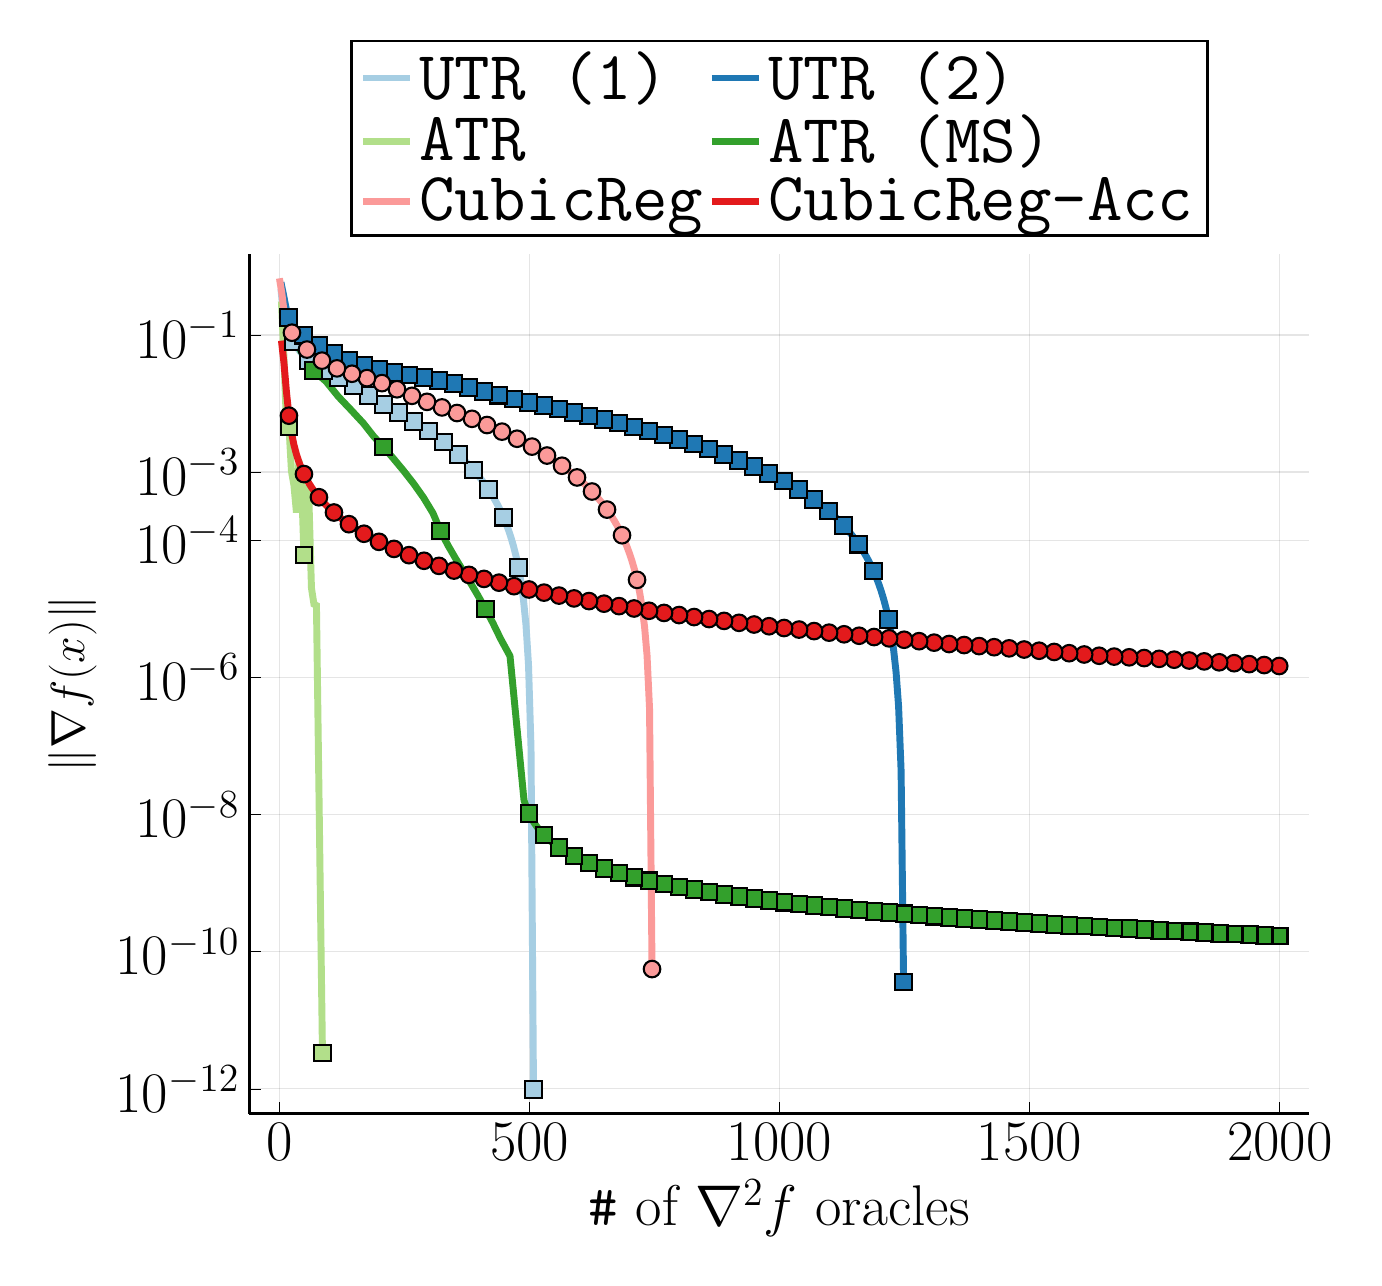
\begin{tikzpicture}[/tikz/background rectangle/.style={fill={rgb,1:red,1.0;green,1.0;blue,1.0}, fill opacity={1.0}, draw opacity={1.0}}, show background rectangle]
\begin{axis}[point meta max={nan}, point meta min={nan}, legend cell align={left}, legend columns={2}, title={}, title style={at={{(0.5,1)}}, anchor={south}, font={{\fontsize{22 pt}{28.6 pt}\selectfont}}, color={rgb,1:red,0.0;green,0.0;blue,0.0}, draw opacity={1.0}, rotate={0.0}, align={center}}, legend style={color={rgb,1:red,0.0;green,0.0;blue,0.0}, draw opacity={1.0}, line width={1}, solid, fill={rgb,1:red,1.0;green,1.0;blue,1.0}, fill opacity={0.7}, text opacity={1.0}, font={{\fontsize{24 pt}{31.200000000000003 pt}\selectfont}}, text={rgb,1:red,0.0;green,0.0;blue,0.0}, cells={anchor={west}}, at={(0.5, 1.02)}, anchor={south}}, axis background/.style={fill={rgb,1:red,1.0;green,1.0;blue,1.0}, opacity={1.0}}, anchor={north west}, xshift={1.0mm}, yshift={-1.0mm}, width={150.4mm}, height={125.0mm}, scaled x ticks={false}, xlabel={\texttt{\#} of $\nabla^2f$ oracles}, x tick style={color={rgb,1:red,0.0;green,0.0;blue,0.0}, opacity={1.0}}, x tick label style={color={rgb,1:red,0.0;green,0.0;blue,0.0}, opacity={1.0}, rotate={0}}, xlabel style={at={(ticklabel cs:0.5)}, anchor=near ticklabel, at={{(ticklabel cs:0.5)}}, anchor={near ticklabel}, font={{\fontsize{20 pt}{26.0 pt}\selectfont}}, color={rgb,1:red,0.0;green,0.0;blue,0.0}, draw opacity={1.0}, rotate={0.0}}, xmajorgrids={true}, xmin={-59.97000000000003}, xmax={2058.9700000000003}, xticklabels={{$0$,$500$,$1000$,$1500$,$2000$}}, xtick={{0.0,500.0,1000.0,1500.0,2000.0}}, xtick align={inside}, xticklabel style={font={{\fontsize{20 pt}{26.0 pt}\selectfont}}, color={rgb,1:red,0.0;green,0.0;blue,0.0}, draw opacity={1.0}, rotate={0.0}}, x grid style={color={rgb,1:red,0.0;green,0.0;blue,0.0}, draw opacity={0.1}, line width={0.5}, solid}, axis x line*={left}, x axis line style={color={rgb,1:red,0.0;green,0.0;blue,0.0}, draw opacity={1.0}, line width={1}, solid}, scaled y ticks={false}, ylabel={$\|\nabla f(x)\|$}, y tick style={color={rgb,1:red,0.0;green,0.0;blue,0.0}, opacity={1.0}}, y tick label style={color={rgb,1:red,0.0;green,0.0;blue,0.0}, opacity={1.0}, rotate={0}}, ylabel style={at={(ticklabel cs:0.5)}, anchor=near ticklabel, at={{(ticklabel cs:0.5)}}, anchor={near ticklabel}, font={{\fontsize{17 pt}{22.1 pt}\selectfont}}, color={rgb,1:red,0.0;green,0.0;blue,0.0}, draw opacity={1.0}, rotate={0.0}}, ymode={log}, log basis y={10}, ymajorgrids={true}, ymin={4.3278033936164226e-13}, ymax={1.5121021166652058}, yticklabels={{$10^{-12}$,$10^{-10}$,$10^{-8}$,$10^{-6}$,$10^{-4}$,$10^{-3}$,$10^{-1}$}}, ytick={{1.0e-12,1.0e-10,1.0e-8,1.0e-6,0.0001,0.001,0.1}}, ytick align={inside}, yticklabel style={font={{\fontsize{20 pt}{26.0 pt}\selectfont}}, color={rgb,1:red,0.0;green,0.0;blue,0.0}, draw opacity={1.0}, rotate={0.0}}, y grid style={color={rgb,1:red,0.0;green,0.0;blue,0.0}, draw opacity={0.1}, line width={0.5}, solid}, axis y line*={left}, y axis line style={color={rgb,1:red,0.0;green,0.0;blue,0.0}, draw opacity={1.0}, line width={1}, solid}, colorbar={false}]
    \addplot[color={rgb,1:red,0.651;green,0.808;blue,0.89}, name path={49}, draw opacity={1.0}, line width={2.5}, solid]
        table[row sep={\\}]
        {
            \\
            508.0  9.800922714868468e-13  \\
            503.0  9.567605204308365e-8  \\
            498.0  1.5351457897981046e-6  \\
            493.0  5.783662441346151e-6  \\
            488.0  1.3450574872230631e-5  \\
            483.0  2.4823258219746227e-5  \\
            478.0  4.007454531392731e-5  \\
            473.0  5.932476554221499e-5  \\
            468.0  8.266550213177431e-5  \\
            463.0  0.0001101706824407824  \\
            458.0  0.00014190264526609938  \\
            453.0  0.0001779160006477503  \\
            448.0  0.00021826051616447093  \\
            443.0  0.00026298366475604253  \\
            438.0  0.00031213321572719086  \\
            433.0  0.0003657601282458458  \\
            428.0  0.0004239219276415145  \\
            423.0  0.0004866866625009307  \\
            418.0  0.0005541374216837981  \\
            413.0  0.0006263772075983761  \\
            408.0  0.0007035336972213015  \\
            403.0  0.0007857630786932713  \\
            398.0  0.0008732517739020921  \\
            393.0  0.0009662145563725864  \\
            388.0  0.0010648875364425744  \\
            383.0  0.0011695149529132032  \\
            378.0  0.0012803298871555482  \\
            373.0  0.0013975309089004687  \\
            368.0  0.0015212588975259478  \\
            363.0  0.0016515800315424886  \\
            358.0  0.0017884811363700064  \\
            353.0  0.0019318814678452485  \\
            348.0  0.002081660774125983  \\
            343.0  0.0022376984973584467  \\
            338.0  0.0023999152915859475  \\
            333.0  0.002568307282616341  \\
            328.0  0.002742966011767832  \\
            323.0  0.0029240816824403046  \\
            318.0  0.0031119322186385656  \\
            313.0  0.0033068638536627353  \\
            308.0  0.00350926944606199  \\
            303.0  0.0037195686482976954  \\
            298.0  0.003938190647342721  \\
            293.0  0.004165557126788482  \\
            288.0  0.004402061941586475  \\
            283.0  0.004648045861364354  \\
            278.0  0.00490376982597582  \\
            273.0  0.005169396983572677  \\
            268.0  0.0054449985642523605  \\
            263.0  0.005730596221774947  \\
            258.0  0.006026240858224598  \\
            253.0  0.006332108815806325  \\
            248.0  0.006648581638256689  \\
            243.0  0.006976277130304271  \\
            238.0  0.0073160206442414236  \\
            233.0  0.0076687784066543  \\
            228.0  0.008035604209928288  \\
            223.0  0.008417660621975373  \\
            218.0  0.008816353423652787  \\
            213.0  0.009233561945955709  \\
            208.0  0.00967187934754173  \\
            203.0  0.010134760325342997  \\
            198.0  0.010626600839061017  \\
            193.0  0.011152911063636226  \\
            188.0  0.011720373684800505  \\
            183.0  0.012335925901401472  \\
            178.0  0.013004615741926002  \\
            173.0  0.013727917436215265  \\
            168.0  0.014504014441972392  \\
            163.0  0.015328644961022233  \\
            158.0  0.016195093276063402  \\
            153.0  0.017093689012974905  \\
            148.0  0.018012609873925473  \\
            143.0  0.01894010415589069  \\
            138.0  0.019866234858823967  \\
            133.0  0.020783900064121414  \\
            128.0  0.021689205535495262  \\
            123.0  0.022581856068675566  \\
            118.0  0.023465816835647132  \\
            113.0  0.024349608489310826  \\
            108.0  0.025247540399425242  \\
            103.0  0.02618162118552048  \\
            98.0  0.027181916513918825  \\
            93.0  0.028282860323462646  \\
            88.0  0.02952213158789623  \\
            83.0  0.030942285660574404  \\
            78.0  0.03259086867410773  \\
            73.0  0.03450190809134403  \\
            68.0  0.03672790336828366  \\
            63.0  0.039334559932278704  \\
            58.0  0.04229168712834866  \\
            53.0  0.04568553525333707  \\
            48.0  0.049868412169536656  \\
            43.0  0.055007133131067705  \\
            38.0  0.06124694042612741  \\
            33.0  0.06895852873370326  \\
            28.0  0.07859852615310098  \\
            23.0  0.09098958835300977  \\
            18.0  0.1071520692610964  \\
            13.0  0.12840741122226712  \\
            8.0  0.18858674645189408  \\
            3.0  0.47376884456356844  \\
        }
        ;
    \addlegendentry {$\texttt{UTR (1)}$}
    \addplot[color={rgb,1:red,0.8889;green,0.4356;blue,0.2781}, name path={50}, only marks, draw opacity={1.0}, line width={0}, solid, mark={square*}, mark size={3.0 pt}, mark repeat={1}, mark options={color={rgb,1:red,0.0;green,0.0;blue,0.0}, draw opacity={1.0}, fill={rgb,1:red,0.651;green,0.808;blue,0.89}, fill opacity={1.0}, line width={0.75}, rotate={0}, solid}, forget plot]
        table[row sep={\\}]
        {
            \\
            508.0  9.800922714868468e-13  \\
            478.0  4.007454531392731e-5  \\
            448.0  0.00021826051616447093  \\
            418.0  0.0005541374216837981  \\
            388.0  0.0010648875364425744  \\
            358.0  0.0017884811363700064  \\
            328.0  0.002742966011767832  \\
            298.0  0.003938190647342721  \\
            268.0  0.0054449985642523605  \\
            238.0  0.0073160206442414236  \\
            208.0  0.00967187934754173  \\
            178.0  0.013004615741926002  \\
            148.0  0.018012609873925473  \\
            118.0  0.023465816835647132  \\
            88.0  0.02952213158789623  \\
            58.0  0.04229168712834866  \\
            28.0  0.07859852615310098  \\
        }
        ;
    \addplot[color={rgb,1:red,0.122;green,0.471;blue,0.706}, name path={51}, draw opacity={1.0}, line width={2.5}, solid]
        table[row sep={\\}]
        {
            \\
            1248.0  3.624325016759895e-11  \\
            1243.0  4.3722931838431515e-8  \\
            1238.0  3.785858287295696e-7  \\
            1233.0  1.190413451058327e-6  \\
            1228.0  2.551191589122859e-6  \\
            1223.0  4.496043194863704e-6  \\
            1218.0  7.046305594979224e-6  \\
            1213.0  1.0216814796121783e-5  \\
            1208.0  1.4018814701270773e-5  \\
            1203.0  1.8461334562723786e-5  \\
            1198.0  2.3551925141885987e-5  \\
            1193.0  2.9297089069308746e-5  \\
            1188.0  3.570255045305226e-5  \\
            1183.0  4.2773433384708815e-5  \\
            1178.0  5.051438566518848e-5  \\
            1173.0  5.892966800108507e-5  \\
            1168.0  6.802322060648899e-5  \\
            1163.0  7.779871458528954e-5  \\
            1158.0  8.825959284440442e-5  \\
            1153.0  9.940910371486868e-5  \\
            1148.0  0.00011125032948136361  \\
            1143.0  0.0001237862113970433  \\
            1138.0  0.00013701957235232626  \\
            1133.0  0.00015095313809381273  \\
            1128.0  0.00016558955770456073  \\
            1123.0  0.00018093142392955997  \\
            1118.0  0.0001969812938414636  \\
            1113.0  0.00021374171027837237  \\
            1108.0  0.0002312152244391947  \\
            1103.0  0.00024940441998619095  \\
            1098.0  0.0002683119389740971  \\
            1093.0  0.00028794050989637885  \\
            1088.0  0.0003082929781085685  \\
            1083.0  0.0003293723388526033  \\
            1078.0  0.0003511817730618635  \\
            1073.0  0.00037372468607076045  \\
            1068.0  0.0003970047492822327  \\
            1063.0  0.00042102594475824354  \\
            1058.0  0.00044579261258914817  \\
            1053.0  0.00047130950076494833  \\
            1048.0  0.0004975818171124481  \\
            1043.0  0.0005246152826755266  \\
            1038.0  0.0005524161857005983  \\
            1033.0  0.0005809914351465397  \\
            1028.0  0.000610348612371034  \\
            1023.0  0.0006404960193585231  \\
            1018.0  0.0006714427215576314  \\
            1013.0  0.0007031985830999247  \\
            1008.0  0.0007357742918938003  \\
            1003.0  0.0007691813718478293  \\
            998.0  0.0008034321793023484  \\
            993.0  0.0008385398806657647  \\
            988.0  0.0008745184082955567  \\
            983.0  0.0009113823918671348  \\
            978.0  0.0009491470628699252  \\
            973.0  0.0009878281304883507  \\
            968.0  0.0010274416279871035  \\
            963.0  0.001068003729833886  \\
            958.0  0.0011095305411501573  \\
            953.0  0.0011520378626509449  \\
            948.0  0.0011955409359624815  \\
            943.0  0.001240054176007971  \\
            938.0  0.0012855908989167282  \\
            933.0  0.0013321630555070108  \\
            928.0  0.0013797809816688917  \\
            923.0  0.0014284531777779153  \\
            918.0  0.0014781861294607779  \\
            913.0  0.0015289841814968477  \\
            908.0  0.0015808494753048717  \\
            903.0  0.0016337819583242992  \\
            898.0  0.0016877794707172386  \\
            893.0  0.0017428379113266842  \\
            888.0  0.001798951480934457  \\
            883.0  0.0018561129968273427  \\
            878.0  0.0019143142687929684  \\
            873.0  0.0019735465232216484  \\
            868.0  0.0020338008592537295  \\
            863.0  0.002095068719096708  \\
            858.0  0.00215734235388012  \\
            853.0  0.002220615266769999  \\
            848.0  0.0022848826164907493  \\
            843.0  0.0023501415667821746  \\
            838.0  0.0024163915704681284  \\
            833.0  0.0024836345804977776  \\
            828.0  0.002551875184279853  \\
            823.0  0.0026211206615945858  \\
            818.0  0.002691380970077177  \\
            813.0  0.0027626686654865238  \\
            808.0  0.0028349987665103943  \\
            803.0  0.0029083885755746  \\
            798.0  0.002982857467942566  \\
            793.0  0.0030584266613047756  \\
            788.0  0.0031351189771219473  \\
            783.0  0.003212958603317248  \\
            778.0  0.0032919708656727496  \\
            773.0  0.0033721820126660766  \\
            768.0  0.00345361901569259  \\
            763.0  0.0035363093838661212  \\
            758.0  0.003620280990079555  \\
            753.0  0.0037055619029235163  \\
            748.0  0.0037921802175786947  \\
            743.0  0.0038801638780672624  \\
            738.0  0.003969540483402615  \\
            733.0  0.004060337071317249  \\
            728.0  0.004152579875440721  \\
            723.0  0.004246294055052571  \\
            718.0  0.004341503400780552  \\
            713.0  0.0044382300246821075  \\
            708.0  0.004536494048739349  \\
            703.0  0.004636313311475142  \\
            698.0  0.004737703117575936  \\
            693.0  0.0048406760593824  \\
            688.0  0.004945241941111885  \\
            683.0  0.005051407835963444  \\
            678.0  0.005159178302226482  \\
            673.0  0.005268555776850123  \\
            668.0  0.0053795411537253  \\
            663.0  0.005492134539781619  \\
            658.0  0.0056063361660287  \\
            653.0  0.005722147414454376  \\
            648.0  0.005839571907095653  \\
            643.0  0.005958616592529656  \\
            638.0  0.00607929275915682  \\
            633.0  0.006201616905132667  \\
            628.0  0.0063256114021295546  \\
            623.0  0.006451304904010757  \\
            618.0  0.006578732471024151  \\
            613.0  0.006707935403792424  \\
            608.0  0.0068389608073892005  \\
            603.0  0.0069718609322144175  \\
            598.0  0.007106692363285119  \\
            593.0  0.007243515151056721  \\
            588.0  0.007382391993142531  \\
            583.0  0.007523387585497619  \\
            578.0  0.007666568262064334  \\
            573.0  0.007812002032109394  \\
            568.0  0.007959759103653692  \\
            563.0  0.008109912949506007  \\
            558.0  0.008262541930475155  \\
            553.0  0.00841773144031342  \\
            548.0  0.00857557648160361  \\
            543.0  0.008736184524922998  \\
            538.0  0.008899678451061313  \\
            533.0  0.009066199337794978  \\
            528.0  0.009235908844794975  \\
            523.0  0.00940899099460108  \\
            518.0  0.009585653266167712  \\
            513.0  0.009766127117464735  \\
            508.0  0.009950668303368654  \\
            503.0  0.010139557559572117  \\
            498.0  0.01033310222397423  \\
            493.0  0.01053163900103627  \\
            488.0  0.010735537298332464  \\
            483.0  0.01094520157106868  \\
            478.0  0.011161070314501802  \\
            473.0  0.011383609190429477  \\
            468.0  0.011613296504808796  \\
            463.0  0.011850600835470737  \\
            458.0  0.01209595281539137  \\
            453.0  0.012349715494072756  \\
            448.0  0.012612159505665544  \\
            443.0  0.012883449150325231  \\
            438.0  0.013163642394662415  \\
            433.0  0.013452702455058425  \\
            428.0  0.013750514070641259  \\
            423.0  0.01405689703259066  \\
            418.0  0.014371613279151754  \\
            413.0  0.014694368351958703  \\
            408.0  0.015024809063893385  \\
            403.0  0.015362517088671519  \\
            398.0  0.015706998111357725  \\
            393.0  0.016057671045735127  \\
            388.0  0.016413866217565354  \\
            383.0  0.016774838532605762  \\
            378.0  0.01713979339826602  \\
            373.0  0.017507917335675475  \\
            368.0  0.017878405596257457  \\
            363.0  0.01825048333145564  \\
            358.0  0.01862342112943163  \\
            353.0  0.01899654766829952  \\
            348.0  0.019369261234043783  \\
            343.0  0.01974103927681593  \\
            338.0  0.020111443752450827  \\
            333.0  0.020480121545907417  \\
            328.0  0.020846802878099056  \\
            323.0  0.021211302990243368  \\
            318.0  0.021573530488457816  \\
            313.0  0.021933499875864158  \\
            308.0  0.022291341004377435  \\
            303.0  0.022647300057815796  \\
            298.0  0.023001734708114903  \\
            293.0  0.023355112644067443  \\
            288.0  0.023708020846836462  \\
            283.0  0.024061184797423668  \\
            278.0  0.024415491244679424  \\
            273.0  0.024772010060499134  \\
            268.0  0.025132015322180474  \\
            263.0  0.025497005824583398  \\
            258.0  0.025868717942590446  \\
            253.0  0.02624911328920538  \\
            248.0  0.026640325074170947  \\
            243.0  0.027044577215211685  \\
            238.0  0.02746413078624481  \\
            233.0  0.027901301986026784  \\
            228.0  0.028358520528877534  \\
            223.0  0.028838352416808575  \\
            218.0  0.02934346810120801  \\
            213.0  0.029876633650749784  \\
            208.0  0.030440831546129882  \\
            203.0  0.03103940628845664  \\
            198.0  0.03167570915315688  \\
            193.0  0.03235210372032939  \\
            188.0  0.03306983256616987  \\
            183.0  0.03383072432524821  \\
            178.0  0.034638429171936394  \\
            173.0  0.035497562701036996  \\
            168.0  0.03641230917542454  \\
            163.0  0.03738722068164696  \\
            158.0  0.03842722638182069  \\
            153.0  0.03953181892294348  \\
            148.0  0.0406899790424437  \\
            143.0  0.04189259342167485  \\
            138.0  0.043150229338425314  \\
            133.0  0.044493341276605175  \\
            128.0  0.045955723732682814  \\
            123.0  0.04755104939166622  \\
            118.0  0.04928822782179941  \\
            113.0  0.051178848346589735  \\
            108.0  0.053226387383134705  \\
            103.0  0.05545264071152326  \\
            98.0  0.05786009126265625  \\
            93.0  0.06044697065005972  \\
            88.0  0.06326821058229563  \\
            83.0  0.06635812091968087  \\
            78.0  0.06974385020123917  \\
            73.0  0.07346006173229527  \\
            68.0  0.07748857831126083  \\
            63.0  0.0820244713657529  \\
            58.0  0.08708350391970536  \\
            53.0  0.0925214565589739  \\
            48.0  0.09884067223748653  \\
            43.0  0.10574431996502437  \\
            38.0  0.11325846527724916  \\
            33.0  0.1215646857733058  \\
            28.0  0.131634773829369  \\
            23.0  0.14697897227079815  \\
            18.0  0.17905869058361523  \\
            13.0  0.251888765724871  \\
            8.0  0.3883271339825141  \\
            3.0  0.5827075891766592  \\
        }
        ;
    \addlegendentry {$\texttt{UTR (2)}$}
    \addplot[color={rgb,1:red,0.7644;green,0.4441;blue,0.8243}, name path={52}, only marks, draw opacity={1.0}, line width={0}, solid, mark={square*}, mark size={3.0 pt}, mark repeat={1}, mark options={color={rgb,1:red,0.0;green,0.0;blue,0.0}, draw opacity={1.0}, fill={rgb,1:red,0.122;green,0.471;blue,0.706}, fill opacity={1.0}, line width={0.75}, rotate={0}, solid}, forget plot]
        table[row sep={\\}]
        {
            \\
            1248.0  3.624325016759895e-11  \\
            1218.0  7.046305594979224e-6  \\
            1188.0  3.570255045305226e-5  \\
            1158.0  8.825959284440442e-5  \\
            1128.0  0.00016558955770456073  \\
            1098.0  0.0002683119389740971  \\
            1068.0  0.0003970047492822327  \\
            1038.0  0.0005524161857005983  \\
            1008.0  0.0007357742918938003  \\
            978.0  0.0009491470628699252  \\
            948.0  0.0011955409359624815  \\
            918.0  0.0014781861294607779  \\
            888.0  0.001798951480934457  \\
            858.0  0.00215734235388012  \\
            828.0  0.002551875184279853  \\
            798.0  0.002982857467942566  \\
            768.0  0.00345361901569259  \\
            738.0  0.003969540483402615  \\
            708.0  0.004536494048739349  \\
            678.0  0.005159178302226482  \\
            648.0  0.005839571907095653  \\
            618.0  0.006578732471024151  \\
            588.0  0.007382391993142531  \\
            558.0  0.008262541930475155  \\
            528.0  0.009235908844794975  \\
            498.0  0.01033310222397423  \\
            468.0  0.011613296504808796  \\
            438.0  0.013163642394662415  \\
            408.0  0.015024809063893385  \\
            378.0  0.01713979339826602  \\
            348.0  0.019369261234043783  \\
            318.0  0.021573530488457816  \\
            288.0  0.023708020846836462  \\
            258.0  0.025868717942590446  \\
            228.0  0.028358520528877534  \\
            198.0  0.03167570915315688  \\
            168.0  0.03641230917542454  \\
            138.0  0.043150229338425314  \\
            108.0  0.053226387383134705  \\
            78.0  0.06974385020123917  \\
            48.0  0.09884067223748653  \\
            18.0  0.17905869058361523  \\
        }
        ;
    \addplot[color={rgb,1:red,0.698;green,0.875;blue,0.541}, name path={53}, draw opacity={1.0}, line width={2.5}, solid]
        table[row sep={\\}]
        {
            \\
            86.0  3.344820490277698e-12  \\
            74.0  1.1237823004117479e-5  \\
            69.0  1.1749121480368745e-5  \\
            64.0  2.025375626779366e-5  \\
            59.0  0.000375355506400514  \\
            54.0  0.0006450422190448675  \\
            49.0  6.11842893757361e-5  \\
            44.0  0.0007575696657500818  \\
            39.0  0.0014696017533119203  \\
            34.0  0.000254692453460069  \\
            29.0  0.0006363127159184678  \\
            24.0  0.0010256876408245822  \\
            19.0  0.004620698626934742  \\
            14.0  0.005024875759219763  \\
            9.0  0.04705835872060752  \\
            4.0  0.30599234223989785  \\
        }
        ;
    \addlegendentry {$\texttt{ATR}$}
    \addplot[color={rgb,1:red,0.0;green,0.6658;blue,0.681}, name path={54}, only marks, draw opacity={1.0}, line width={0}, solid, mark={square*}, mark size={3.0 pt}, mark repeat={1}, mark options={color={rgb,1:red,0.0;green,0.0;blue,0.0}, draw opacity={1.0}, fill={rgb,1:red,0.698;green,0.875;blue,0.541}, fill opacity={1.0}, line width={0.75}, rotate={0}, solid}, forget plot]
        table[row sep={\\}]
        {
            \\
            86.0  3.344820490277698e-12  \\
            49.0  6.11842893757361e-5  \\
            19.0  0.004620698626934742  \\
        }
        ;
    \addplot[color={rgb,1:red,0.2;green,0.627;blue,0.173}, name path={55}, draw opacity={1.0}, line width={2.5}, solid]
        table[row sep={\\}]
        {
            \\
            1999.0  1.6936196159182326e-10  \\
            1994.0  1.7000247176307762e-10  \\
            1989.0  1.7064402914248358e-10  \\
            1984.0  1.712910972887295e-10  \\
            1979.0  1.7193951031039132e-10  \\
            1974.0  1.72593664062782e-10  \\
            1969.0  1.7325249981131288e-10  \\
            1964.0  1.739176241690227e-10  \\
            1959.0  1.7458300972648722e-10  \\
            1954.0  1.7525388629349006e-10  \\
            1949.0  1.7593169690885953e-10  \\
            1944.0  1.7661579338407198e-10  \\
            1939.0  1.7730099634736473e-10  \\
            1934.0  1.7799327948404734e-10  \\
            1929.0  1.7868958889249934e-10  \\
            1924.0  1.7939026825857884e-10  \\
            1919.0  1.8009691964212032e-10  \\
            1914.0  1.8080786792161091e-10  \\
            1909.0  1.8152329009333894e-10  \\
            1904.0  1.8224530337160748e-10  \\
            1899.0  1.829728066396548e-10  \\
            1894.0  1.8370483750215609e-10  \\
            1889.0  1.8444111457943795e-10  \\
            1884.0  1.851835717234043e-10  \\
            1879.0  1.8593103185198797e-10  \\
            1874.0  1.8668301964686084e-10  \\
            1869.0  1.874412165873965e-10  \\
            1864.0  1.882047281967435e-10  \\
            1859.0  1.8897430193175857e-10  \\
            1854.0  1.8974906460382587e-10  \\
            1849.0  1.9053057777789223e-10  \\
            1844.0  1.9131621429012777e-10  \\
            1839.0  1.9210713641387478e-10  \\
            1834.0  1.9290393045415915e-10  \\
            1829.0  1.9370715948168846e-10  \\
            1824.0  1.945166454341453e-10  \\
            1819.0  1.953327573125161e-10  \\
            1814.0  1.9615456279338568e-10  \\
            1809.0  1.9698220349627723e-10  \\
            1804.0  1.9781575412998426e-10  \\
            1799.0  1.9865740777402637e-10  \\
            1794.0  1.995044382615219e-10  \\
            1789.0  2.0035494852392764e-10  \\
            1784.0  2.0121346381064265e-10  \\
            1779.0  2.0208063475883345e-10  \\
            1774.0  2.0295438047513268e-10  \\
            1769.0  2.0383296241838364e-10  \\
            1764.0  2.0471975879492294e-10  \\
            1759.0  2.0561451110080132e-10  \\
            1754.0  2.0651525247138461e-10  \\
            1749.0  2.0742253103992262e-10  \\
            1744.0  2.0833477621600016e-10  \\
            1739.0  2.092547374534242e-10  \\
            1734.0  2.101823785717886e-10  \\
            1729.0  2.1111982779994453e-10  \\
            1724.0  2.1206393426345754e-10  \\
            1719.0  2.1301568078156255e-10  \\
            1714.0  2.1397362702200788e-10  \\
            1709.0  2.149396390556918e-10  \\
            1704.0  2.1591331206751382e-10  \\
            1699.0  2.168963573988168e-10  \\
            1694.0  2.1788718727344396e-10  \\
            1689.0  2.1888664396569106e-10  \\
            1684.0  2.1989087098713323e-10  \\
            1679.0  2.2090671440678e-10  \\
            1674.0  2.21931723570055e-10  \\
            1669.0  2.2296669012267858e-10  \\
            1664.0  2.2400862110181317e-10  \\
            1659.0  2.250596674315481e-10  \\
            1654.0  2.2611897201717229e-10  \\
            1649.0  2.271859512187642e-10  \\
            1644.0  2.2826518748086875e-10  \\
            1639.0  2.2935080741756997e-10  \\
            1634.0  2.3044687790711603e-10  \\
            1629.0  2.3155309383202873e-10  \\
            1624.0  2.3266811611085542e-10  \\
            1619.0  2.337947594156167e-10  \\
            1614.0  2.3492781943830295e-10  \\
            1609.0  2.36072061979563e-10  \\
            1604.0  2.3722688777686103e-10  \\
            1599.0  2.3839143057948857e-10  \\
            1594.0  2.3956413069884963e-10  \\
            1589.0  2.4075046863603743e-10  \\
            1584.0  2.41946929887282e-10  \\
            1579.0  2.431533999442141e-10  \\
            1574.0  2.443723906759624e-10  \\
            1569.0  2.4559962539477416e-10  \\
            1564.0  2.468387090072527e-10  \\
            1559.0  2.4809189296468243e-10  \\
            1554.0  2.493559212512902e-10  \\
            1549.0  2.5063061261706687e-10  \\
            1544.0  2.519175750317456e-10  \\
            1539.0  2.5321864308847865e-10  \\
            1534.0  2.545313119041001e-10  \\
            1529.0  2.5585420123224263e-10  \\
            1524.0  2.5719070546028336e-10  \\
            1519.0  2.5853913975419714e-10  \\
            1514.0  2.599011619348731e-10  \\
            1509.0  2.6127553137705585e-10  \\
            1504.0  2.6266613409175965e-10  \\
            1499.0  2.6406761252647295e-10  \\
            1494.0  2.6548164082262477e-10  \\
            1489.0  2.669118562644132e-10  \\
            1484.0  2.6835464683969877e-10  \\
            1479.0  2.698140046515998e-10  \\
            1474.0  2.7128463338909097e-10  \\
            1469.0  2.72772289510598e-10  \\
            1464.0  2.742728632000279e-10  \\
            1459.0  2.7578967946140586e-10  \\
            1454.0  2.773233168577138e-10  \\
            1449.0  2.788729039672293e-10  \\
            1444.0  2.8043814033919384e-10  \\
            1439.0  2.8201933163630644e-10  \\
            1434.0  2.83617703734717e-10  \\
            1429.0  2.8523154283725524e-10  \\
            1424.0  2.868615704230201e-10  \\
            1419.0  2.8850836448585346e-10  \\
            1414.0  2.901737563180668e-10  \\
            1409.0  2.91858685011911e-10  \\
            1404.0  2.9355876673992375e-10  \\
            1399.0  2.952798720313243e-10  \\
            1394.0  2.970164024849584e-10  \\
            1389.0  2.987748639503621e-10  \\
            1384.0  3.005532826007122e-10  \\
            1379.0  3.0235002451744486e-10  \\
            1374.0  3.041670915779199e-10  \\
            1369.0  3.060018845964015e-10  \\
            1364.0  3.0785885967467183e-10  \\
            1359.0  3.0973724936320236e-10  \\
            1354.0  3.1163424024417085e-10  \\
            1349.0  3.135564202671453e-10  \\
            1344.0  3.1549971446602903e-10  \\
            1339.0  3.1746687070989447e-10  \\
            1334.0  3.194559386796376e-10  \\
            1329.0  3.214692494065719e-10  \\
            1324.0  3.2350622529649947e-10  \\
            1319.0  3.255637248506877e-10  \\
            1314.0  3.276458417982915e-10  \\
            1309.0  3.2975409077608364e-10  \\
            1304.0  3.318882050790032e-10  \\
            1299.0  3.3404690756200316e-10  \\
            1294.0  3.362315366887694e-10  \\
            1289.0  3.384447049583795e-10  \\
            1284.0  3.4068545895080383e-10  \\
            1279.0  3.4295420371791907e-10  \\
            1274.0  3.452486303902774e-10  \\
            1269.0  3.4757564417978015e-10  \\
            1264.0  3.499306950624899e-10  \\
            1259.0  3.5231501434724883e-10  \\
            1254.0  3.547279294067148e-10  \\
            1249.0  3.5717409265285677e-10  \\
            1244.0  3.5965102239128313e-10  \\
            1239.0  3.621603187928867e-10  \\
            1234.0  3.6470385386076726e-10  \\
            1229.0  3.6727989552276165e-10  \\
            1224.0  3.698881852903954e-10  \\
            1219.0  3.725329302000052e-10  \\
            1214.0  3.752131591406752e-10  \\
            1209.0  3.779297055853831e-10  \\
            1204.0  3.806834908382031e-10  \\
            1199.0  3.8347368581218936e-10  \\
            1194.0  3.8630250329361976e-10  \\
            1189.0  3.891734304166924e-10  \\
            1184.0  3.920827726343771e-10  \\
            1179.0  3.950339630906828e-10  \\
            1174.0  3.980278330567224e-10  \\
            1169.0  4.010620334338933e-10  \\
            1164.0  4.0414264838998644e-10  \\
            1159.0  4.072660747513573e-10  \\
            1154.0  4.104356467826785e-10  \\
            1149.0  4.136518399042156e-10  \\
            1144.0  4.169159731281806e-10  \\
            1139.0  4.202293519489002e-10  \\
            1134.0  4.235911368315416e-10  \\
            1129.0  4.2700547282709446e-10  \\
            1124.0  4.304689004063638e-10  \\
            1119.0  4.339877997192034e-10  \\
            1114.0  4.375625961739603e-10  \\
            1109.0  4.4119138339378376e-10  \\
            1104.0  4.4487563675230775e-10  \\
            1099.0  4.4862137531448236e-10  \\
            1094.0  4.5242649269810215e-10  \\
            1089.0  4.562912660726535e-10  \\
            1084.0  4.6022034685286743e-10  \\
            1079.0  4.6421509508606824e-10  \\
            1074.0  4.682754134761031e-10  \\
            1069.0  4.724033558295561e-10  \\
            1064.0  4.766012177501253e-10  \\
            1059.0  4.808699377324138e-10  \\
            1054.0  4.852112957194995e-10  \\
            1049.0  4.896273304205787e-10  \\
            1044.0  4.941217871551839e-10  \\
            1039.0  4.986953329050882e-10  \\
            1034.0  5.03348150221805e-10  \\
            1029.0  5.080857691318054e-10  \\
            1024.0  5.129099803658632e-10  \\
            1019.0  5.178191641505237e-10  \\
            1014.0  5.22819457650826e-10  \\
            1009.0  5.279129490555034e-10  \\
            1004.0  5.331013459264244e-10  \\
            999.0  5.383888674563747e-10  \\
            994.0  5.437778052509606e-10  \\
            989.0  5.492702166318224e-10  \\
            984.0  5.548691170906712e-10  \\
            979.0  5.605786110182048e-10  \\
            974.0  5.664008569208718e-10  \\
            969.0  5.723389269033306e-10  \\
            964.0  5.78395897853569e-10  \\
            959.0  5.845783393672709e-10  \\
            954.0  5.908902861510776e-10  \\
            949.0  5.973288523594823e-10  \\
            944.0  6.039065140036127e-10  \\
            939.0  6.106249169980866e-10  \\
            934.0  6.174858183778518e-10  \\
            929.0  6.244959302820144e-10  \\
            924.0  6.316633790600403e-10  \\
            919.0  6.389898273306348e-10  \\
            914.0  6.464786848115799e-10  \\
            909.0  6.541398259139957e-10  \\
            904.0  6.619758036109542e-10  \\
            899.0  6.699964151000598e-10  \\
            894.0  6.782062081210228e-10  \\
            889.0  6.866115035611265e-10  \\
            884.0  6.952191037363559e-10  \\
            879.0  7.040370564252301e-10  \\
            874.0  7.130731253924005e-10  \\
            869.0  7.223359729616281e-10  \\
            864.0  7.318313499195068e-10  \\
            859.0  7.415736088191757e-10  \\
            854.0  7.515702896038239e-10  \\
            849.0  7.618280588990842e-10  \\
            844.0  7.723580468116053e-10  \\
            839.0  7.831753851823324e-10  \\
            834.0  7.942893975310299e-10  \\
            829.0  8.057138554747164e-10  \\
            824.0  8.17459933920699e-10  \\
            819.0  8.295406881004721e-10  \\
            814.0  8.419728689064088e-10  \\
            809.0  8.547726606767213e-10  \\
            804.0  8.679533659695351e-10  \\
            799.0  8.815355865635024e-10  \\
            794.0  8.955365442357814e-10  \\
            789.0  9.099737840861743e-10  \\
            784.0  9.248719946502224e-10  \\
            779.0  9.402517720762957e-10  \\
            774.0  9.56137814415182e-10  \\
            769.0  9.725552280995571e-10  \\
            764.0  9.895265924603456e-10  \\
            759.0  1.0070867250598501e-9  \\
            754.0  1.0252652700888912e-9  \\
            749.0  1.0440944846835386e-9  \\
            744.0  1.0636101397467822e-9  \\
            739.0  1.0838503452327197e-9  \\
            734.0  1.104857160879722e-9  \\
            729.0  1.126673821678289e-9  \\
            724.0  1.1493470363152894e-9  \\
            719.0  1.1729298496520868e-9  \\
            714.0  1.197480284220291e-9  \\
            709.0  1.2230560039566403e-9  \\
            704.0  1.249723431549929e-9  \\
            699.0  1.2775554171843727e-9  \\
            694.0  1.3066289278872966e-9  \\
            689.0  1.3370278633733317e-9  \\
            684.0  1.3688468254814461e-9  \\
            679.0  1.4021853991203289e-9  \\
            674.0  1.4371574482058414e-9  \\
            669.0  1.4738874082364096e-9  \\
            664.0  1.512508443512406e-9  \\
            659.0  1.5531722019972354e-9  \\
            654.0  1.5960455545814324e-9  \\
            649.0  1.6413129292851425e-9  \\
            644.0  1.6891811202448822e-9  \\
            639.0  1.7398801992318466e-9  \\
            634.0  1.7936706152741972e-9  \\
            629.0  1.850843119802218e-9  \\
            624.0  1.91172865079917e-9  \\
            619.0  1.9767000321905822e-9  \\
            614.0  2.0461843293828804e-9  \\
            609.0  2.1206693265788823e-9  \\
            604.0  2.200717371509613e-9  \\
            599.0  2.2869730165985248e-9  \\
            594.0  2.3801912999232594e-9  \\
            589.0  2.481251812288065e-9  \\
            584.0  2.5911899861488007e-9  \\
            579.0  2.7112304694021736e-9  \\
            574.0  2.842836004089966e-9  \\
            569.0  2.987765395397633e-9  \\
            564.0  3.14815464282097e-9  \\
            559.0  3.3266214738817853e-9  \\
            554.0  3.526412519290389e-9  \\
            549.0  3.7516031827092984e-9  \\
            544.0  4.007379381374658e-9  \\
            539.0  4.300445125157378e-9  \\
            534.0  4.639622857230417e-9  \\
            529.0  5.036763986784325e-9  \\
            524.0  5.5081761613081375e-9  \\
            519.0  6.0769359898407256e-9  \\
            514.0  6.776821221531038e-9  \\
            509.0  7.659355715142097e-9  \\
            504.0  8.807269904982229e-9  \\
            499.0  1.0362783146610622e-8  \\
            494.0  1.2592847244942212e-8  \\
            489.0  1.6165487759957278e-8  \\
            461.0  2.059935407852045e-6  \\
            442.0  3.698371733907842e-6  \\
            427.0  6.208771688041422e-6  \\
            412.0  1.001331716278295e-5  \\
            397.0  1.5669574467772423e-5  \\
            382.0  2.3996232463340896e-5  \\
            367.0  3.629480188865958e-5  \\
            352.0  5.490816087206485e-5  \\
            337.0  8.477347388163248e-5  \\
            322.0  0.00013813224325844508  \\
            307.0  0.00025010082952352106  \\
            288.0  0.0004232424752803725  \\
            268.0  0.0006801142067371706  \\
            248.0  0.0010445435389971364  \\
            228.0  0.0015666175466265448  \\
            208.0  0.002302541383618761  \\
            188.0  0.003332497787880993  \\
            168.0  0.005110900166763329  \\
            143.0  0.008043182377834296  \\
            118.0  0.012501569587773311  \\
            93.0  0.020949335947169263  \\
            68.0  0.03018154669175811  \\
            43.0  0.05730439876376935  \\
            18.0  0.15276798467838573  \\
        }
        ;
    \addlegendentry {$\texttt{ATR (MS)}$}
    \addplot[color={rgb,1:red,0.777;green,0.5097;blue,0.1464}, name path={56}, only marks, draw opacity={1.0}, line width={0}, solid, mark={square*}, mark size={3.0 pt}, mark repeat={1}, mark options={color={rgb,1:red,0.0;green,0.0;blue,0.0}, draw opacity={1.0}, fill={rgb,1:red,0.2;green,0.627;blue,0.173}, fill opacity={1.0}, line width={0.75}, rotate={0}, solid}, forget plot]
        table[row sep={\\}]
        {
            \\
            1999.0  1.6936196159182326e-10  \\
            1969.0  1.7325249981131288e-10  \\
            1939.0  1.7730099634736473e-10  \\
            1909.0  1.8152329009333894e-10  \\
            1879.0  1.8593103185198797e-10  \\
            1849.0  1.9053057777789223e-10  \\
            1819.0  1.953327573125161e-10  \\
            1789.0  2.0035494852392764e-10  \\
            1759.0  2.0561451110080132e-10  \\
            1729.0  2.1111982779994453e-10  \\
            1699.0  2.168963573988168e-10  \\
            1669.0  2.2296669012267858e-10  \\
            1639.0  2.2935080741756997e-10  \\
            1609.0  2.36072061979563e-10  \\
            1579.0  2.431533999442141e-10  \\
            1549.0  2.5063061261706687e-10  \\
            1519.0  2.5853913975419714e-10  \\
            1489.0  2.669118562644132e-10  \\
            1459.0  2.7578967946140586e-10  \\
            1429.0  2.8523154283725524e-10  \\
            1399.0  2.952798720313243e-10  \\
            1369.0  3.060018845964015e-10  \\
            1339.0  3.1746687070989447e-10  \\
            1309.0  3.2975409077608364e-10  \\
            1279.0  3.4295420371791907e-10  \\
            1249.0  3.5717409265285677e-10  \\
            1219.0  3.725329302000052e-10  \\
            1189.0  3.891734304166924e-10  \\
            1159.0  4.072660747513573e-10  \\
            1129.0  4.2700547282709446e-10  \\
            1099.0  4.4862137531448236e-10  \\
            1069.0  4.724033558295561e-10  \\
            1039.0  4.986953329050882e-10  \\
            1009.0  5.279129490555034e-10  \\
            979.0  5.605786110182048e-10  \\
            949.0  5.973288523594823e-10  \\
            919.0  6.389898273306348e-10  \\
            889.0  6.866115035611265e-10  \\
            859.0  7.415736088191757e-10  \\
            829.0  8.057138554747164e-10  \\
            799.0  8.815355865635024e-10  \\
            769.0  9.725552280995571e-10  \\
            739.0  1.0838503452327197e-9  \\
            709.0  1.2230560039566403e-9  \\
            679.0  1.4021853991203289e-9  \\
            649.0  1.6413129292851425e-9  \\
            619.0  1.9767000321905822e-9  \\
            589.0  2.481251812288065e-9  \\
            559.0  3.3266214738817853e-9  \\
            529.0  5.036763986784325e-9  \\
            499.0  1.0362783146610622e-8  \\
            412.0  1.001331716278295e-5  \\
            322.0  0.00013813224325844508  \\
            208.0  0.002302541383618761  \\
            68.0  0.03018154669175811  \\
        }
        ;
    \addplot[color={rgb,1:red,0.984;green,0.604;blue,0.6}, name path={57}, draw opacity={1.0}, line width={2.5}, solid]
        table[row sep={\\}]
        {
            \\
            745.0  5.5846669453766193e-11  \\
            740.0  3.5276058460040574e-7  \\
            735.0  2.114764211471125e-6  \\
            730.0  5.560837347775903e-6  \\
            725.0  1.0766538534928159e-5  \\
            720.0  1.7774189086936927e-5  \\
            715.0  2.661497766748116e-5  \\
            710.0  3.7310565202612055e-5  \\
            705.0  4.9883429022735425e-5  \\
            700.0  6.435139423500778e-5  \\
            695.0  8.072885300984625e-5  \\
            690.0  9.903053334003222e-5  \\
            685.0  0.00011927100215948448  \\
            680.0  0.00014146100411639354  \\
            675.0  0.0001656121924175451  \\
            670.0  0.00019173674492571985  \\
            665.0  0.00021984534207839817  \\
            660.0  0.00024994846836156166  \\
            655.0  0.00028205918222905593  \\
            650.0  0.00031618904662749194  \\
            645.0  0.00035235188861358987  \\
            640.0  0.00039056333683786974  \\
            635.0  0.0004308401892690907  \\
            630.0  0.0004732033027952038  \\
            625.0  0.0005176763287496995  \\
            620.0  0.0005642863032135505  \\
            615.0  0.0006130643735238232  \\
            610.0  0.0006640524571076762  \\
            605.0  0.0007172914593025102  \\
            600.0  0.0007728306232060252  \\
            595.0  0.0008307301844374484  \\
            590.0  0.0008910499265381323  \\
            585.0  0.0009538585803979474  \\
            580.0  0.001019229263323343  \\
            575.0  0.0010872352690836922  \\
            570.0  0.0011579532421564108  \\
            565.0  0.001231449482058724  \\
            560.0  0.0013077914956728064  \\
            555.0  0.0013870316525547966  \\
            550.0  0.001469211806044201  \\
            545.0  0.0015543583599967993  \\
            540.0  0.0016424781979982742  \\
            535.0  0.0017335634715461433  \\
            530.0  0.0018275895618928974  \\
            525.0  0.001924524725947373  \\
            520.0  0.002024326260518545  \\
            515.0  0.002126956291704088  \\
            510.0  0.0022323794086921396  \\
            505.0  0.0023405720956026542  \\
            500.0  0.002451528045944986  \\
            495.0  0.0025652567183047604  \\
            490.0  0.002681787889478263  \\
            485.0  0.0028011786639363123  \\
            480.0  0.002923497513604214  \\
            475.0  0.003048836172969651  \\
            470.0  0.00317729456857666  \\
            465.0  0.003308985521438204  \\
            460.0  0.0034440309675137287  \\
            455.0  0.003582558139409443  \\
            450.0  0.00372469627950158  \\
            445.0  0.0038705756046852054  \\
            440.0  0.004020323912731146  \\
            435.0  0.004174066517099343  \\
            430.0  0.004331921782173613  \\
            425.0  0.004493992125852293  \\
            420.0  0.004660371694785984  \\
            415.0  0.004831130971135466  \\
            410.0  0.005006320576569873  \\
            405.0  0.005185974007428913  \\
            400.0  0.005370102541613471  \\
            395.0  0.005558710319681797  \\
            390.0  0.005751799743431415  \\
            385.0  0.005949390497423931  \\
            380.0  0.006151527120905276  \\
            375.0  0.006358294581575959  \\
            370.0  0.006569823052514984  \\
            365.0  0.006786295551904869  \\
            360.0  0.007007932904359754  \\
            355.0  0.0072350015411145946  \\
            350.0  0.00746778880655399  \\
            345.0  0.007706600880972053  \\
            340.0  0.007951755603367269  \\
            335.0  0.008203595429945513  \\
            330.0  0.008462497772492915  \\
            325.0  0.008728911456069476  \\
            320.0  0.009003383419669681  \\
            315.0  0.009286600839604689  \\
            310.0  0.009579415926062006  \\
            305.0  0.009882863851368327  \\
            300.0  0.010198167788257993  \\
            295.0  0.010526749679170092  \\
            290.0  0.010870268569362384  \\
            285.0  0.01123064476360673  \\
            280.0  0.011610019215270306  \\
            275.0  0.012010563488050971  \\
            270.0  0.012434154894091942  \\
            265.0  0.012882037967038894  \\
            260.0  0.013354661684988547  \\
            255.0  0.013851748183064153  \\
            250.0  0.014372460945733224  \\
            245.0  0.014915510686689795  \\
            240.0  0.0154791353302383  \\
            235.0  0.01606101589195968  \\
            230.0  0.016658175176582586  \\
            225.0  0.01726709465603101  \\
            220.0  0.01788403731155076  \\
            215.0  0.0185053844713478  \\
            210.0  0.01912786566945521  \\
            205.0  0.019748720755201035  \\
            200.0  0.020365815846676287  \\
            195.0  0.020977668465416953  \\
            190.0  0.02158345772882361  \\
            185.0  0.022183124886049378  \\
            180.0  0.022777486075955408  \\
            175.0  0.0233682355178629  \\
            170.0  0.023957972063053896  \\
            165.0  0.024550389434696437  \\
            160.0  0.02515055923056615  \\
            155.0  0.025765196842575517  \\
            150.0  0.026402796727517504  \\
            145.0  0.027073228535091455  \\
            140.0  0.0277869474741162  \\
            135.0  0.02855495578298956  \\
            130.0  0.02938919880110861  \\
            125.0  0.030302523187398105  \\
            120.0  0.031309576653153315  \\
            115.0  0.03242467530107629  \\
            110.0  0.03365599766323822  \\
            105.0  0.035016412598835846  \\
            100.0  0.03652609895135895  \\
            95.0  0.03820610663825528  \\
            90.0  0.040065475515781025  \\
            85.0  0.042064939174968764  \\
            80.0  0.044236986826350376  \\
            75.0  0.046720938335390844  \\
            70.0  0.04958933865986004  \\
            65.0  0.0528875903022082  \\
            60.0  0.05667024949947504  \\
            55.0  0.06096195189196557  \\
            50.0  0.06592263949106722  \\
            45.0  0.07171168770862636  \\
            40.0  0.07841544490841876  \\
            35.0  0.08652012747569642  \\
            30.0  0.09598830692309065  \\
            25.0  0.10748232466286635  \\
            20.0  0.12087753056320649  \\
            15.0  0.14034176312073718  \\
            10.0  0.19726539513149843  \\
            5.0  0.39478701195987587  \\
            0.0  0.6677004668214126  \\
        }
        ;
    \addlegendentry {$\texttt{CubicReg}$}
    \addplot[color={rgb,1:red,0.5585;green,0.5935;blue,0.1175}, name path={58}, only marks, draw opacity={1.0}, line width={0}, solid, mark={*}, mark size={3.0 pt}, mark repeat={1}, mark options={color={rgb,1:red,0.0;green,0.0;blue,0.0}, draw opacity={1.0}, fill={rgb,1:red,0.984;green,0.604;blue,0.6}, fill opacity={1.0}, line width={0.75}, rotate={0}, solid}, forget plot]
        table[row sep={\\}]
        {
            \\
            745.0  5.5846669453766193e-11  \\
            715.0  2.661497766748116e-5  \\
            685.0  0.00011927100215948448  \\
            655.0  0.00028205918222905593  \\
            625.0  0.0005176763287496995  \\
            595.0  0.0008307301844374484  \\
            565.0  0.001231449482058724  \\
            535.0  0.0017335634715461433  \\
            505.0  0.0023405720956026542  \\
            475.0  0.003048836172969651  \\
            445.0  0.0038705756046852054  \\
            415.0  0.004831130971135466  \\
            385.0  0.005949390497423931  \\
            355.0  0.0072350015411145946  \\
            325.0  0.008728911456069476  \\
            295.0  0.010526749679170092  \\
            265.0  0.012882037967038894  \\
            235.0  0.01606101589195968  \\
            205.0  0.019748720755201035  \\
            175.0  0.0233682355178629  \\
            145.0  0.027073228535091455  \\
            115.0  0.03242467530107629  \\
            85.0  0.042064939174968764  \\
            55.0  0.06096195189196557  \\
            25.0  0.10748232466286635  \\
        }
        ;
    \addplot[color={rgb,1:red,0.89;green,0.102;blue,0.11}, name path={59}, draw opacity={1.0}, line width={2.5}, solid]
        table[row sep={\\}]
        {
            \\
            1999.0  1.4734004052630673e-6  \\
            1994.0  1.4813530566095335e-6  \\
            1989.0  1.4893304981723102e-6  \\
            1984.0  1.4973323800325432e-6  \\
            1979.0  1.5053583430897321e-6  \\
            1974.0  1.513408026623187e-6  \\
            1969.0  1.5214810334050116e-6  \\
            1964.0  1.529576973665265e-6  \\
            1959.0  1.5376954232072644e-6  \\
            1954.0  1.5458359519381571e-6  \\
            1949.0  1.5539981167628832e-6  \\
            1944.0  1.5621814387213492e-6  \\
            1939.0  1.5703854586555806e-6  \\
            1934.0  1.5786096642795922e-6  \\
            1929.0  1.5868535422187876e-6  \\
            1924.0  1.5951165552120104e-6  \\
            1919.0  1.603398127803553e-6  \\
            1914.0  1.6116977211327687e-6  \\
            1909.0  1.6200147161199076e-6  \\
            1904.0  1.628348520880851e-6  \\
            1899.0  1.6366984876491144e-6  \\
            1894.0  1.645063981052668e-6  \\
            1889.0  1.6534443065127744e-6  \\
            1884.0  1.661838761601819e-6  \\
            1879.0  1.6702466202254264e-6  \\
            1874.0  1.678667154156182e-6  \\
            1869.0  1.6870995674054022e-6  \\
            1864.0  1.6955430791936366e-6  \\
            1859.0  1.703996852591871e-6  \\
            1854.0  1.7124600486207545e-6  \\
            1849.0  1.7209318024191312e-6  \\
            1844.0  1.7294111953003665e-6  \\
            1839.0  1.7378973129242081e-6  \\
            1834.0  1.746389182932174e-6  \\
            1829.0  1.7548858098036293e-6  \\
            1824.0  1.7633861826013375e-6  \\
            1819.0  1.7718892427610287e-6  \\
            1814.0  1.7803939053679727e-6  \\
            1809.0  1.7888990579564097e-6  \\
            1804.0  1.797403551489572e-6  \\
            1799.0  1.8059061978518145e-6  \\
            1794.0  1.814405769922508e-6  \\
            1789.0  1.8229010248306846e-6  \\
            1784.0  1.8313906638110347e-6  \\
            1779.0  1.8398733606857285e-6  \\
            1774.0  1.8483477488632182e-6  \\
            1769.0  1.8568123931086888e-6  \\
            1764.0  1.8652658741739599e-6  \\
            1759.0  1.8737066821749253e-6  \\
            1754.0  1.8821332996693772e-6  \\
            1749.0  1.890544129875784e-6  \\
            1744.0  1.898937571173078e-6  \\
            1739.0  1.907311959449915e-6  \\
            1734.0  1.915665574403259e-6  \\
            1729.0  1.9239966534966986e-6  \\
            1724.0  1.932303391832213e-6  \\
            1719.0  1.940583945468813e-6  \\
            1714.0  1.948836419184127e-6  \\
            1709.0  1.957058846972265e-6  \\
            1704.0  1.96524921756824e-6  \\
            1699.0  1.9734054636456594e-6  \\
            1694.0  1.981525487630132e-6  \\
            1689.0  1.9896071340228235e-6  \\
            1684.0  1.9976481492112045e-6  \\
            1679.0  2.005646271870213e-6  \\
            1674.0  2.0135991835079786e-6  \\
            1669.0  2.0215044770107443e-6  \\
            1664.0  2.029359700168167e-6  \\
            1659.0  2.0371623544474593e-6  \\
            1654.0  2.044909861509068e-6  \\
            1649.0  2.0525995840546927e-6  \\
            1644.0  2.063317007265617e-6  \\
            1639.0  2.0783664041593883e-6  \\
            1634.0  2.093494632432026e-6  \\
            1629.0  2.108701289826494e-6  \\
            1624.0  2.1239859238550025e-6  \\
            1619.0  2.1393480513756328e-6  \\
            1614.0  2.154787166604929e-6  \\
            1609.0  2.1703027329618673e-6  \\
            1604.0  2.1858941584493716e-6  \\
            1599.0  2.2015608207201732e-6  \\
            1594.0  2.2173020538107406e-6  \\
            1589.0  2.233117171551137e-6  \\
            1584.0  2.2490054071283736e-6  \\
            1579.0  2.2649659586475502e-6  \\
            1574.0  2.280998006973552e-6  \\
            1569.0  2.297100668785976e-6  \\
            1564.0  2.3132729879628413e-6  \\
            1559.0  2.329513987066805e-6  \\
            1554.0  2.345822640225966e-6  \\
            1549.0  2.3621978359640585e-6  \\
            1544.0  2.3786384289656612e-6  \\
            1539.0  2.395143215439243e-6  \\
            1534.0  2.4117109163944975e-6  \\
            1529.0  2.4283401979917686e-6  \\
            1524.0  2.4450296749085756e-6  \\
            1519.0  2.4617778674030777e-6  \\
            1514.0  2.478583229561317e-6  \\
            1509.0  2.495444169915696e-6  \\
            1504.0  2.5123590015424082e-6  \\
            1499.0  2.5293259610744907e-6  \\
            1494.0  2.546343196140006e-6  \\
            1489.0  2.5634087902107907e-6  \\
            1484.0  2.580520744194294e-6  \\
            1479.0  2.5976769415141713e-6  \\
            1474.0  2.61487521409374e-6  \\
            1469.0  2.6321132631616966e-6  \\
            1464.0  2.6493887245088027e-6  \\
            1459.0  2.6666991087841886e-6  \\
            1454.0  2.6840418321408914e-6  \\
            1449.0  2.701414202528632e-6  \\
            1444.0  2.7188134093695892e-6  \\
            1439.0  2.7362365476108754e-6  \\
            1434.0  2.753680571895942e-6  \\
            1429.0  2.7711423258105683e-6  \\
            1424.0  2.7886185230295706e-6  \\
            1419.0  2.8061057633837834e-6  \\
            1414.0  2.82360049588834e-6  \\
            1409.0  2.8410990356033862e-6  \\
            1404.0  2.858597555204786e-6  \\
            1399.0  2.8760920825454763e-6  \\
            1394.0  2.8935784876631583e-6  \\
            1389.0  2.9110524965916745e-6  \\
            1384.0  2.9285096649440977e-6  \\
            1379.0  2.9459453946602043e-6  \\
            1374.0  2.9633549185732194e-6  \\
            1369.0  2.980733295987021e-6  \\
            1364.0  2.9980753768457634e-6  \\
            1359.0  3.0153758751036203e-6  \\
            1354.0  3.0326292898071418e-6  \\
            1349.0  3.049829917216484e-6  \\
            1344.0  3.0669718806062555e-6  \\
            1339.0  3.0840490805036367e-6  \\
            1334.0  3.101055366824529e-6  \\
            1329.0  3.125529654369206e-6  \\
            1324.0  3.1517572075693865e-6  \\
            1319.0  3.1781216771991687e-6  \\
            1314.0  3.2046208968961653e-6  \\
            1309.0  3.2312525544773246e-6  \\
            1304.0  3.2580142016671788e-6  \\
            1299.0  3.2849032349776147e-6  \\
            1294.0  3.3119168863176116e-6  \\
            1289.0  3.3390522170582912e-6  \\
            1284.0  3.3663061351853475e-6  \\
            1279.0  3.3936753598516708e-6  \\
            1274.0  3.4211564190989956e-6  \\
            1269.0  3.4487456561061795e-6  \\
            1264.0  3.4764392052743185e-6  \\
            1259.0  3.5042330027577785e-6  \\
            1254.0  3.5321227561274806e-6  \\
            1249.0  3.560103929743081e-6  \\
            1244.0  3.5881717838261803e-6  \\
            1239.0  3.6163213126790572e-6  \\
            1234.0  3.6445472679143408e-6  \\
            1229.0  3.672844127474091e-6  \\
            1224.0  3.701206099666311e-6  \\
            1219.0  3.729627097887419e-6  \\
            1214.0  3.7581007400471063e-6  \\
            1209.0  3.786620353254683e-6  \\
            1204.0  3.815178903443227e-6  \\
            1199.0  3.84376906843567e-6  \\
            1194.0  3.872383154628006e-6  \\
            1189.0  3.901013137701404e-6  \\
            1184.0  3.9296505989456305e-6  \\
            1179.0  3.958286743988336e-6  \\
            1174.0  3.986912380613635e-6  \\
            1169.0  4.015517905061177e-6  \\
            1164.0  4.044093305139968e-6  \\
            1159.0  4.072628090899739e-6  \\
            1154.0  4.101111362424836e-6  \\
            1149.0  4.1295317168555925e-6  \\
            1144.0  4.16025541067972e-6  \\
            1139.0  4.199254747228919e-6  \\
            1134.0  4.238459405044829e-6  \\
            1129.0  4.277863883600176e-6  \\
            1124.0  4.317462294591178e-6  \\
            1119.0  4.357248379172511e-6  \\
            1114.0  4.397215460110994e-6  \\
            1109.0  4.437356456515106e-6  \\
            1104.0  4.4776638283028575e-6  \\
            1099.0  4.5181296118802815e-6  \\
            1094.0  4.5587453225407526e-6  \\
            1089.0  4.599501987733245e-6  \\
            1084.0  4.6403901169727045e-6  \\
            1079.0  4.681399657588869e-6  \\
            1074.0  4.722519989274508e-6  \\
            1069.0  4.763739890186339e-6  \\
            1064.0  4.805047538258815e-6  \\
            1059.0  4.846430418147374e-6  \\
            1054.0  4.887875374418455e-6  \\
            1049.0  4.9293685236290355e-6  \\
            1044.0  4.9708952407372285e-6  \\
            1039.0  5.012440157868439e-6  \\
            1034.0  5.053987077605969e-6  \\
            1029.0  5.0955189934048855e-6  \\
            1024.0  5.137018033688539e-6  \\
            1019.0  5.1784654160740954e-6  \\
            1014.0  5.227307083308802e-6  \\
            1009.0  5.2807854873694824e-6  \\
            1004.0  5.334539873320917e-6  \\
            999.0  5.388558874022219e-6  \\
            994.0  5.442830342939869e-6  \\
            989.0  5.497341313249248e-6  \\
            984.0  5.552077931445394e-6  \\
            979.0  5.607025428422249e-6  \\
            974.0  5.662168089056692e-6  \\
            969.0  5.7174891778362425e-6  \\
            964.0  5.772970930834886e-6  \\
            959.0  5.828594448494878e-6  \\
            954.0  5.884339680573524e-6  \\
            949.0  5.940185363011028e-6  \\
            944.0  5.996108966354415e-6  \\
            939.0  6.052086625078259e-6  \\
            934.0  6.108093082594849e-6  \\
            929.0  6.164101627852555e-6  \\
            924.0  6.220084689679751e-6  \\
            919.0  6.286865180346024e-6  \\
            914.0  6.356191072983528e-6  \\
            909.0  6.425870461235738e-6  \\
            904.0  6.4958835657449e-6  \\
            899.0  6.5662091554791955e-6  \\
            894.0  6.636824492193327e-6  \\
            889.0  6.707705197855277e-6  \\
            884.0  6.778825230353868e-6  \\
            879.0  6.8501567542833254e-6  \\
            874.0  6.921670073275327e-6  \\
            869.0  6.993333494868696e-6  \\
            864.0  7.065113273074535e-6  \\
            859.0  7.136973476699656e-6  \\
            854.0  7.208875884655212e-6  \\
            849.0  7.28403458780069e-6  \\
            844.0  7.370181489825907e-6  \\
            839.0  7.4567865579395355e-6  \\
            834.0  7.543820260752102e-6  \\
            829.0  7.631250774963822e-6  \\
            824.0  7.719043842869912e-6  \\
            819.0  7.807162617102003e-6  \\
            814.0  7.895567542236936e-6  \\
            809.0  7.984216170262961e-6  \\
            804.0  8.073063025004812e-6  \\
            799.0  8.162059442711313e-6  \\
            794.0  8.251153369834002e-6  \\
            789.0  8.346809849733765e-6  \\
            784.0  8.451341533108981e-6  \\
            779.0  8.556423160831112e-6  \\
            774.0  8.662010799136355e-6  \\
            769.0  8.768056945880848e-6  \\
            764.0  8.874510277885105e-6  \\
            759.0  8.981315449845477e-6  \\
            754.0  9.088412834137496e-6  \\
            749.0  9.195738286606428e-6  \\
            744.0  9.303222887530276e-6  \\
            739.0  9.420962158341938e-6  \\
            734.0  9.545055264015494e-6  \\
            729.0  9.669787086639695e-6  \\
            724.0  9.795095028194854e-6  \\
            719.0  9.920911185610333e-6  \\
            714.0  1.0047161974899446e-5  \\
            709.0  1.0173767822768349e-5  \\
            704.0  1.0300642737899334e-5  \\
            699.0  1.0435048637284547e-5  \\
            694.0  1.0579458786335341e-5  \\
            689.0  1.0724632102217869e-5  \\
            684.0  1.0870486087359475e-5  \\
            679.0  1.1016930905658034e-5  \\
            674.0  1.116386887438378e-5  \\
            669.0  1.131119396585491e-5  \\
            664.0  1.1466531844850473e-5  \\
            659.0  1.1632418940889295e-5  \\
            654.0  1.1799196302238216e-5  \\
            649.0  1.196675720761666e-5  \\
            644.0  1.2134985038900456e-5  \\
            639.0  1.2303752575114022e-5  \\
            634.0  1.2477355284716256e-5  \\
            629.0  1.2665566539848156e-5  \\
            624.0  1.2854816143117053e-5  \\
            619.0  1.3044970413642373e-5  \\
            614.0  1.3235882766137498e-5  \\
            609.0  1.3427395849750138e-5  \\
            604.0  1.3635592174809782e-5  \\
            599.0  1.384794247348811e-5  \\
            594.0  1.4061378724151403e-5  \\
            589.0  1.4275725152047647e-5  \\
            584.0  1.449170296067733e-5  \\
            579.0  1.4727380260751016e-5  \\
            574.0  1.496443660718451e-5  \\
            569.0  1.5202673630443525e-5  \\
            564.0  1.5441872389902698e-5  \\
            559.0  1.569513299415374e-5  \\
            554.0  1.5957047632682354e-5  \\
            549.0  1.6220350045293838e-5  \\
            544.0  1.648478420011276e-5  \\
            539.0  1.676388788147163e-5  \\
            534.0  1.705200067907735e-5  \\
            529.0  1.7341614679413294e-5  \\
            524.0  1.7637860226222642e-5  \\
            519.0  1.7951965458129118e-5  \\
            514.0  1.8267908276503237e-5  \\
            509.0  1.858535177698184e-5  \\
            504.0  1.892325002827813e-5  \\
            499.0  1.926649534493657e-5  \\
            494.0  1.9611465133165642e-5  \\
            489.0  1.9977624666531235e-5  \\
            484.0  2.03493751102114e-5  \\
            479.0  2.072896382006079e-5  \\
            474.0  2.112829870418079e-5  \\
            469.0  2.1530026525864115e-5  \\
            464.0  2.194960332741591e-5  \\
            459.0  2.2380153799077416e-5  \\
            454.0  2.2819393311353768e-5  \\
            449.0  2.3279622887043192e-5  \\
            444.0  2.3744108543778635e-5  \\
            439.0  2.4235050204736982e-5  \\
            434.0  2.4729139823146107e-5  \\
            429.0  2.5248172908674635e-5  \\
            424.0  2.577577277082976e-5  \\
            419.0  2.6331324242218486e-5  \\
            414.0  2.6897535655612524e-5  \\
            409.0  2.7487348168463444e-5  \\
            404.0  2.809362563124337e-5  \\
            399.0  2.8718793608621844e-5  \\
            394.0  2.937213055424948e-5  \\
            389.0  3.0041340277700357e-5  \\
            384.0  3.0736080398324715e-5  \\
            379.0  3.146063219108077e-5  \\
            374.0  3.220801416149651e-5  \\
            369.0  3.297866782359015e-5  \\
            364.0  3.378266062073297e-5  \\
            359.0  3.4618986300586796e-5  \\
            354.0  3.54863187907119e-5  \\
            349.0  3.638527577125185e-5  \\
            344.0  3.7316429364795935e-5  \\
            339.0  3.828664037100673e-5  \\
            334.0  3.929689443629482e-5  \\
            329.0  4.034812419364569e-5  \\
            324.0  4.144118741708333e-5  \\
            319.0  4.258364979599931e-5  \\
            314.0  4.377000833738581e-5  \\
            309.0  4.500793524565202e-5  \\
            304.0  4.6301496366326936e-5  \\
            299.0  4.765337137058525e-5  \\
            294.0  4.906800511981562e-5  \\
            289.0  5.055005983330959e-5  \\
            284.0  5.209519537235211e-5  \\
            279.0  5.3718478754887334e-5  \\
            274.0  5.541912934736803e-5  \\
            269.0  5.720334139528046e-5  \\
            264.0  5.908033342540731e-5  \\
            259.0  6.104942509632756e-5  \\
            254.0  6.312098689773529e-5  \\
            249.0  6.530625904420604e-5  \\
            244.0  6.760433740352622e-5  \\
            239.0  7.003594145008468e-5  \\
            234.0  7.260549229477285e-5  \\
            229.0  7.531731905033893e-5  \\
            224.0  7.819378882897277e-5  \\
            219.0  8.12359203292965e-5  \\
            214.0  8.447288327091842e-5  \\
            209.0  8.791157052263798e-5  \\
            204.0  9.156924525400942e-5  \\
            199.0  9.54683734093446e-5  \\
            194.0  9.96285165547554e-5  \\
            189.0  0.00010406977338792119  \\
            184.0  0.00010883000323960871  \\
            179.0  0.00011393835066982497  \\
            174.0  0.00011942733427289355  \\
            169.0  0.00012534144920522155  \\
            164.0  0.00013172263930641295  \\
            159.0  0.0001386245593282465  \\
            154.0  0.00014609723593859134  \\
            149.0  0.0001542229179758138  \\
            144.0  0.00016307060610837667  \\
            139.0  0.00017277448721979692  \\
            134.0  0.00018339013522564328  \\
            129.0  0.00019506071027715463  \\
            124.0  0.00020794274079721876  \\
            119.0  0.00022221931438552047  \\
            114.0  0.00023809946173126824  \\
            109.0  0.000255859674882779  \\
            104.0  0.0002758133072972814  \\
            99.0  0.0002983729185959857  \\
            94.0  0.0003240483075763245  \\
            89.0  0.0003534666729048625  \\
            84.0  0.0003874502460567702  \\
            79.0  0.00042710590721495913  \\
            74.0  0.00047389948609008134  \\
            69.0  0.0005299309491421455  \\
            64.0  0.0005980271281370744  \\
            59.0  0.0006824921749618116  \\
            54.0  0.0007898071712975814  \\
            49.0  0.0009303203780231707  \\
            44.0  0.0011210882353287052  \\
            39.0  0.0013923112446699154  \\
            34.0  0.0018022864686917893  \\
            29.0  0.0024783115418989124  \\
            24.0  0.0037460733597409384  \\
            19.0  0.006615423385327734  \\
            14.0  0.014761117827736155  \\
            9.0  0.03898276903905969  \\
            4.0  0.0822058693894569  \\
        }
        ;
    \addlegendentry {$\texttt{CubicReg-Acc}$}
    \addplot[color={rgb,1:red,0.6097;green,0.4992;blue,0.9118}, name path={60}, only marks, draw opacity={1.0}, line width={0}, solid, mark={*}, mark size={3.0 pt}, mark repeat={1}, mark options={color={rgb,1:red,0.0;green,0.0;blue,0.0}, draw opacity={1.0}, fill={rgb,1:red,0.89;green,0.102;blue,0.11}, fill opacity={1.0}, line width={0.75}, rotate={0}, solid}, forget plot]
        table[row sep={\\}]
        {
            \\
            1999.0  1.4734004052630673e-6  \\
            1969.0  1.5214810334050116e-6  \\
            1939.0  1.5703854586555806e-6  \\
            1909.0  1.6200147161199076e-6  \\
            1879.0  1.6702466202254264e-6  \\
            1849.0  1.7209318024191312e-6  \\
            1819.0  1.7718892427610287e-6  \\
            1789.0  1.8229010248306846e-6  \\
            1759.0  1.8737066821749253e-6  \\
            1729.0  1.9239966534966986e-6  \\
            1699.0  1.9734054636456594e-6  \\
            1669.0  2.0215044770107443e-6  \\
            1639.0  2.0783664041593883e-6  \\
            1609.0  2.1703027329618673e-6  \\
            1579.0  2.2649659586475502e-6  \\
            1549.0  2.3621978359640585e-6  \\
            1519.0  2.4617778674030777e-6  \\
            1489.0  2.5634087902107907e-6  \\
            1459.0  2.6666991087841886e-6  \\
            1429.0  2.7711423258105683e-6  \\
            1399.0  2.8760920825454763e-6  \\
            1369.0  2.980733295987021e-6  \\
            1339.0  3.0840490805036367e-6  \\
            1309.0  3.2312525544773246e-6  \\
            1279.0  3.3936753598516708e-6  \\
            1249.0  3.560103929743081e-6  \\
            1219.0  3.729627097887419e-6  \\
            1189.0  3.901013137701404e-6  \\
            1159.0  4.072628090899739e-6  \\
            1129.0  4.277863883600176e-6  \\
            1099.0  4.5181296118802815e-6  \\
            1069.0  4.763739890186339e-6  \\
            1039.0  5.012440157868439e-6  \\
            1009.0  5.2807854873694824e-6  \\
            979.0  5.607025428422249e-6  \\
            949.0  5.940185363011028e-6  \\
            919.0  6.286865180346024e-6  \\
            889.0  6.707705197855277e-6  \\
            859.0  7.136973476699656e-6  \\
            829.0  7.631250774963822e-6  \\
            799.0  8.162059442711313e-6  \\
            769.0  8.768056945880848e-6  \\
            739.0  9.420962158341938e-6  \\
            709.0  1.0173767822768349e-5  \\
            679.0  1.1016930905658034e-5  \\
            649.0  1.196675720761666e-5  \\
            619.0  1.3044970413642373e-5  \\
            589.0  1.4275725152047647e-5  \\
            559.0  1.569513299415374e-5  \\
            529.0  1.7341614679413294e-5  \\
            499.0  1.926649534493657e-5  \\
            469.0  2.1530026525864115e-5  \\
            439.0  2.4235050204736982e-5  \\
            409.0  2.7487348168463444e-5  \\
            379.0  3.146063219108077e-5  \\
            349.0  3.638527577125185e-5  \\
            319.0  4.258364979599931e-5  \\
            289.0  5.055005983330959e-5  \\
            259.0  6.104942509632756e-5  \\
            229.0  7.531731905033893e-5  \\
            199.0  9.54683734093446e-5  \\
            169.0  0.00012534144920522155  \\
            139.0  0.00017277448721979692  \\
            109.0  0.000255859674882779  \\
            79.0  0.00042710590721495913  \\
            49.0  0.0009303203780231707  \\
            19.0  0.006615423385327734  \\
        }
        ;
\end{axis}
\end{tikzpicture}
}
    }
    \subcaptionbox{\texttt{w4a}}[0.47\columnwidth]{
        \resizebox{0.47\columnwidth}{!}{% Recommended preamble:
% \usetikzlibrary{arrows.meta}
% \usetikzlibrary{backgrounds}
% \usepgfplotslibrary{patchplots}
% \usepgfplotslibrary{fillbetween}
% \pgfplotsset{%
%     layers/standard/.define layer set={%
%         background,axis background,axis grid,axis ticks,axis lines,axis tick labels,pre main,main,axis descriptions,axis foreground%
%     }{
%         grid style={/pgfplots/on layer=axis grid},%
%         tick style={/pgfplots/on layer=axis ticks},%
%         axis line style={/pgfplots/on layer=axis lines},%
%         label style={/pgfplots/on layer=axis descriptions},%
%         legend style={/pgfplots/on layer=axis descriptions},%
%         title style={/pgfplots/on layer=axis descriptions},%
%         colorbar style={/pgfplots/on layer=axis descriptions},%
%         ticklabel style={/pgfplots/on layer=axis tick labels},%
%         axis background@ style={/pgfplots/on layer=axis background},%
%         3d box foreground style={/pgfplots/on layer=axis foreground},%
%     },
% }

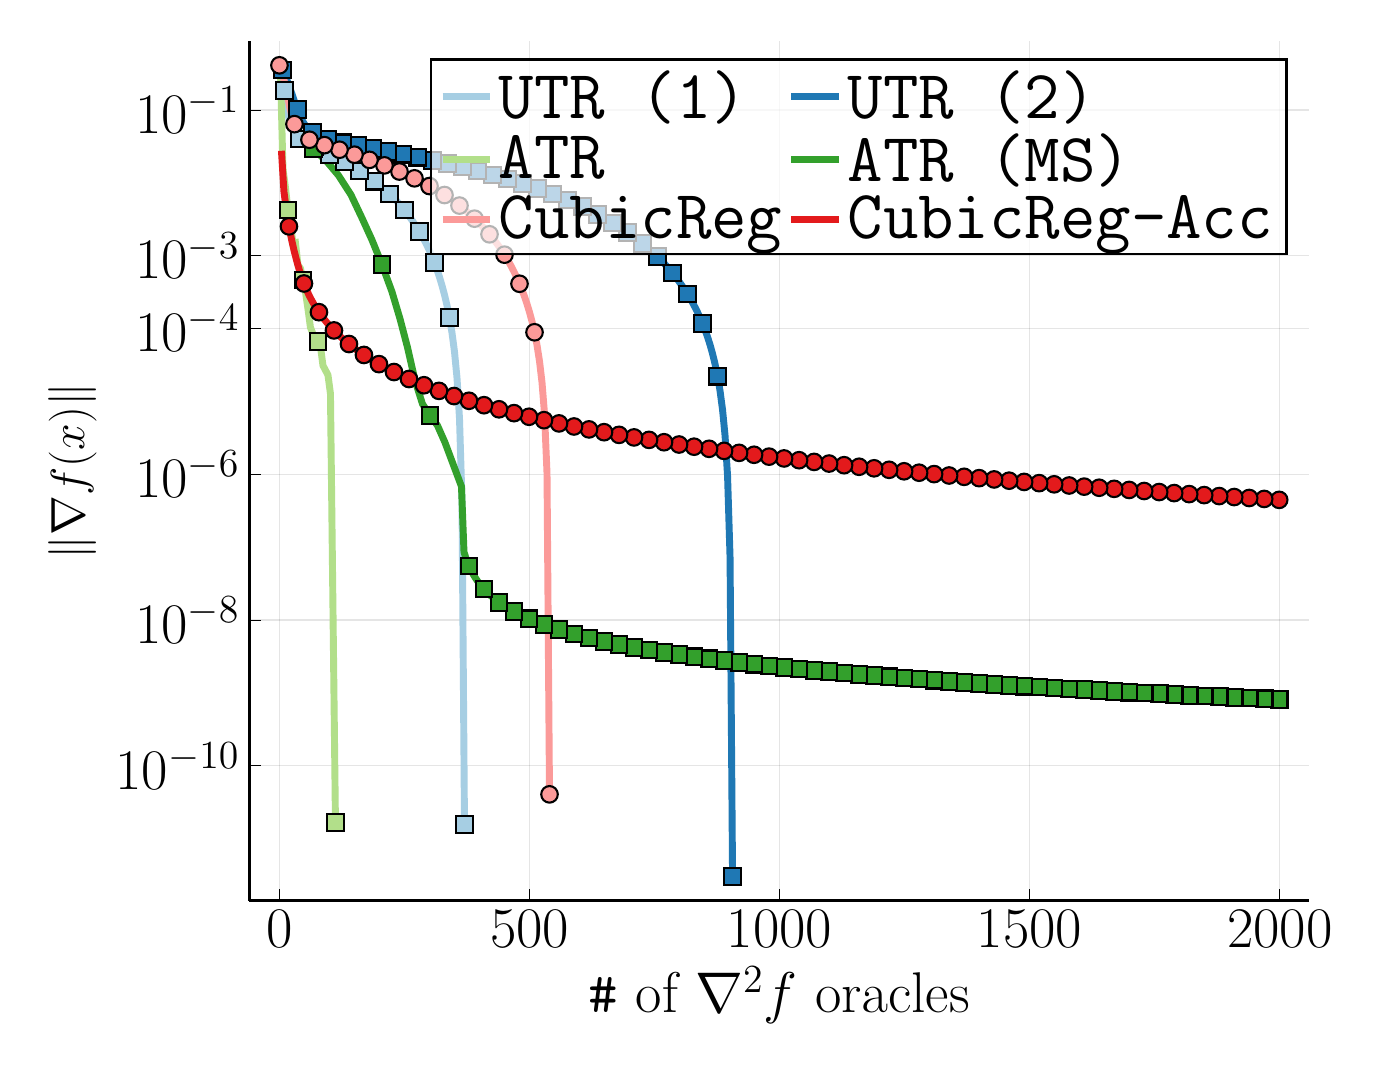
\begin{tikzpicture}[/tikz/background rectangle/.style={fill={rgb,1:red,1.0;green,1.0;blue,1.0}, fill opacity={1.0}, draw opacity={1.0}}, show background rectangle]
\begin{axis}[point meta max={nan}, point meta min={nan}, legend cell align={left}, legend columns={2}, title={}, title style={at={{(0.5,1)}}, anchor={south}, font={{\fontsize{22 pt}{28.6 pt}\selectfont}}, color={rgb,1:red,0.0;green,0.0;blue,0.0}, draw opacity={1.0}, rotate={0.0}, align={center}}, legend style={color={rgb,1:red,0.0;green,0.0;blue,0.0}, draw opacity={1.0}, line width={1}, solid, fill={rgb,1:red,1.0;green,1.0;blue,1.0}, fill opacity={0.7}, text opacity={1.0}, font={{\fontsize{24 pt}{31.200000000000003 pt}\selectfont}}, text={rgb,1:red,0.0;green,0.0;blue,0.0}, cells={anchor={west}}, at={(0.98, 0.98)}, anchor={north east}}, axis background/.style={fill={rgb,1:red,1.0;green,1.0;blue,1.0}, opacity={1.0}}, anchor={north west}, xshift={1.0mm}, yshift={-1.0mm}, width={150.4mm}, height={125.0mm}, scaled x ticks={false}, xlabel={\texttt{\#} of $\nabla^2f$ oracles}, x tick style={color={rgb,1:red,0.0;green,0.0;blue,0.0}, opacity={1.0}}, x tick label style={color={rgb,1:red,0.0;green,0.0;blue,0.0}, opacity={1.0}, rotate={0}}, xlabel style={at={(ticklabel cs:0.5)}, anchor=near ticklabel, at={{(ticklabel cs:0.5)}}, anchor={near ticklabel}, font={{\fontsize{20 pt}{26.0 pt}\selectfont}}, color={rgb,1:red,0.0;green,0.0;blue,0.0}, draw opacity={1.0}, rotate={0.0}}, xmajorgrids={true}, xmin={-59.97000000000003}, xmax={2058.9700000000003}, xticklabels={{$0$,$500$,$1000$,$1500$,$2000$}}, xtick={{0.0,500.0,1000.0,1500.0,2000.0}}, xtick align={inside}, xticklabel style={font={{\fontsize{20 pt}{26.0 pt}\selectfont}}, color={rgb,1:red,0.0;green,0.0;blue,0.0}, draw opacity={1.0}, rotate={0.0}}, x grid style={color={rgb,1:red,0.0;green,0.0;blue,0.0}, draw opacity={0.1}, line width={0.5}, solid}, axis x line*={left}, x axis line style={color={rgb,1:red,0.0;green,0.0;blue,0.0}, draw opacity={1.0}, line width={1}, solid}, scaled y ticks={false}, ylabel={$\|\nabla f(x)\|$}, y tick style={color={rgb,1:red,0.0;green,0.0;blue,0.0}, opacity={1.0}}, y tick label style={color={rgb,1:red,0.0;green,0.0;blue,0.0}, opacity={1.0}, rotate={0}}, ylabel style={at={(ticklabel cs:0.5)}, anchor=near ticklabel, at={{(ticklabel cs:0.5)}}, anchor={near ticklabel}, font={{\fontsize{17 pt}{22.1 pt}\selectfont}}, color={rgb,1:red,0.0;green,0.0;blue,0.0}, draw opacity={1.0}, rotate={0.0}}, ymode={log}, log basis y={10}, ymajorgrids={true}, ymin={1.4063705221966745e-12}, ymax={0.8846972512498897}, yticklabels={{$10^{-10}$,$10^{-8}$,$10^{-6}$,$10^{-4}$,$10^{-3}$,$10^{-1}$}}, ytick={{1.0e-10,1.0e-8,1.0e-6,0.0001,0.001,0.1}}, ytick align={inside}, yticklabel style={font={{\fontsize{20 pt}{26.0 pt}\selectfont}}, color={rgb,1:red,0.0;green,0.0;blue,0.0}, draw opacity={1.0}, rotate={0.0}}, y grid style={color={rgb,1:red,0.0;green,0.0;blue,0.0}, draw opacity={0.1}, line width={0.5}, solid}, axis y line*={left}, y axis line style={color={rgb,1:red,0.0;green,0.0;blue,0.0}, draw opacity={1.0}, line width={1}, solid}, colorbar={false}]
    \addplot[color={rgb,1:red,0.651;green,0.808;blue,0.89}, name path={249}, draw opacity={1.0}, line width={2.5}, solid]
        table[row sep={\\}]
        {
            \\
            370.0  1.5663402262496798e-11  \\
            365.0  4.3632307745602705e-7  \\
            360.0  5.899285010302268e-6  \\
            355.0  2.114500618539772e-5  \\
            350.0  4.807640190148182e-5  \\
            345.0  8.767185195186441e-5  \\
            340.0  0.00014071324405017394  \\
            335.0  0.00020807102243232316  \\
            330.0  0.0002908442805736038  \\
            325.0  0.0003903469581081323  \\
            320.0  0.0005078987712491209  \\
            315.0  0.0006444973089311606  \\
            310.0  0.0008005855183787437  \\
            305.0  0.0009761237403044939  \\
            300.0  0.0011708873009143954  \\
            295.0  0.0013846455756500254  \\
            290.0  0.0016171471601282299  \\
            285.0  0.0018681721758803931  \\
            280.0  0.00213780684482265  \\
            275.0  0.0024268408938268237  \\
            270.0  0.0027370346339329337  \\
            265.0  0.003071084951968965  \\
            260.0  0.003432103191480796  \\
            255.0  0.0038212758685885542  \\
            250.0  0.00423422798920277  \\
            245.0  0.004664836702682163  \\
            240.0  0.005110692198326382  \\
            235.0  0.005571526089525681  \\
            230.0  0.006048119438730957  \\
            225.0  0.006542191615880597  \\
            220.0  0.007055644968482052  \\
            215.0  0.0075892335846832835  \\
            210.0  0.008141822992058585  \\
            205.0  0.008711932415601108  \\
            200.0  0.009299616152242044  \\
            195.0  0.009904771054171911  \\
            190.0  0.01052506737349041  \\
            185.0  0.011158072620214534  \\
            180.0  0.011804293000054653  \\
            175.0  0.012466613978160497  \\
            170.0  0.013148439236422471  \\
            165.0  0.013852941626084768  \\
            160.0  0.014581208336941263  \\
            155.0  0.01533070301401066  \\
            150.0  0.0160975226440137  \\
            145.0  0.016874866337116823  \\
            140.0  0.017660707153070616  \\
            135.0  0.018458833388884124  \\
            130.0  0.019275018898787785  \\
            125.0  0.020115997134692545  \\
            120.0  0.020986261548958652  \\
            115.0  0.021881935866750624  \\
            110.0  0.022792406109153313  \\
            105.0  0.02371486873765764  \\
            100.0  0.02466410105747822  \\
            95.0  0.02564707181846739  \\
            90.0  0.02666611559677226  \\
            85.0  0.027739610241373124  \\
            80.0  0.0288103315499901  \\
            75.0  0.029875145944398444  \\
            70.0  0.030972688411808523  \\
            65.0  0.03209599691615583  \\
            60.0  0.033268996759864326  \\
            55.0  0.03454339796812597  \\
            50.0  0.03595332644514916  \\
            45.0  0.03762303710156709  \\
            40.0  0.03980595023335484  \\
            35.0  0.042864367251856744  \\
            30.0  0.04718647208229487  \\
            25.0  0.054354055600740456  \\
            20.0  0.07000504429429999  \\
            15.0  0.10772483552685981  \\
            10.0  0.18482878047281817  \\
            5.0  0.30174896680170415  \\
            0.0  0.4100807186395152  \\
        }
        ;
    \addlegendentry {$\texttt{UTR (1)}$}
    \addplot[color={rgb,1:red,0.8889;green,0.4356;blue,0.2781}, name path={250}, only marks, draw opacity={1.0}, line width={0}, solid, mark={square*}, mark size={3.0 pt}, mark repeat={1}, mark options={color={rgb,1:red,0.0;green,0.0;blue,0.0}, draw opacity={1.0}, fill={rgb,1:red,0.651;green,0.808;blue,0.89}, fill opacity={1.0}, line width={0.75}, rotate={0}, solid}, forget plot]
        table[row sep={\\}]
        {
            \\
            370.0  1.5663402262496798e-11  \\
            340.0  0.00014071324405017394  \\
            310.0  0.0008005855183787437  \\
            280.0  0.00213780684482265  \\
            250.0  0.00423422798920277  \\
            220.0  0.007055644968482052  \\
            190.0  0.01052506737349041  \\
            160.0  0.014581208336941263  \\
            130.0  0.019275018898787785  \\
            100.0  0.02466410105747822  \\
            70.0  0.030972688411808523  \\
            40.0  0.03980595023335484  \\
            10.0  0.18482878047281817  \\
        }
        ;
    \addplot[color={rgb,1:red,0.122;green,0.471;blue,0.706}, name path={251}, draw opacity={1.0}, line width={2.5}, solid]
        table[row sep={\\}]
        {
            \\
            906.0  3.0340664134467803e-12  \\
            901.0  7.219576249851976e-8  \\
            896.0  9.542698636349088e-7  \\
            891.0  3.3934559869274223e-6  \\
            886.0  7.675298364693903e-6  \\
            881.0  1.3926512292816724e-5  \\
            876.0  2.2219998760724856e-5  \\
            871.0  3.260627597799826e-5  \\
            866.0  4.512573269888318e-5  \\
            861.0  5.9814637812023784e-5  \\
            856.0  7.670875122156545e-5  \\
            851.0  9.584590939253514e-5  \\
            846.0  0.00011726811814604825  \\
            841.0  0.00014102332844835472  \\
            836.0  0.00016716688016873301  \\
            831.0  0.0001957624795050067  \\
            826.0  0.0002268825077519696  \\
            821.0  0.0002606074494829914  \\
            816.0  0.0002970242878173645  \\
            811.0  0.0003362238395177663  \\
            806.0  0.00037829716557562703  \\
            801.0  0.00042333135127262567  \\
            796.0  0.00047140507317936913  \\
            791.0  0.0005225844614362154  \\
            786.0  0.0005769198388524716  \\
            781.0  0.000634443945080683  \\
            776.0  0.0006951721359182405  \\
            771.0  0.0007591046880307837  \\
            766.0  0.0008262307753478897  \\
            761.0  0.0008965331397107738  \\
            756.0  0.0009699922506948244  \\
            751.0  0.0010465889964397105  \\
            746.0  0.0011263055673540253  \\
            741.0  0.0012091248874685353  \\
            736.0  0.0012950294040939016  \\
            731.0  0.0013840001224406642  \\
            726.0  0.0014760165433086426  \\
            721.0  0.0015710578290318198  \\
            716.0  0.0016691052533293197  \\
            711.0  0.0017701458209057502  \\
            706.0  0.0018741768046871853  \\
            701.0  0.001981210780283141  \\
            696.0  0.002091280564444105  \\
            691.0  0.0022044433846859788  \\
            686.0  0.0023207837047386866  \\
            681.0  0.0024404144041155693  \\
            676.0  0.0025634763662390485  \\
            671.0  0.0026901368059371973  \\
            666.0  0.0028205866244205655  \\
            661.0  0.002955036346657621  \\
            656.0  0.0030937082773870492  \\
            651.0  0.0032368191855475553  \\
            646.0  0.0033845445465359664  \\
            641.0  0.0035369578881962955  \\
            636.0  0.003693957109507151  \\
            631.0  0.0038552235018970062  \\
            626.0  0.004020271046441833  \\
            621.0  0.004188583533780818  \\
            616.0  0.004359749600737734  \\
            611.0  0.004533511420098752  \\
            606.0  0.004709734122511025  \\
            601.0  0.004888354734942278  \\
            596.0  0.005069348488361847  \\
            591.0  0.005252716316417942  \\
            586.0  0.005438484172507081  \\
            581.0  0.00562670583064087  \\
            576.0  0.005817464463507338  \\
            571.0  0.006010870645670024  \\
            566.0  0.006207055816615071  \\
            561.0  0.006406161321512118  \\
            556.0  0.0066083240214573555  \\
            551.0  0.00681365998238829  \\
            546.0  0.007022247959731778  \\
            541.0  0.007234114832064661  \\
            536.0  0.007449226650056158  \\
            531.0  0.007667491299543483  \\
            526.0  0.007888778688895422  \\
            521.0  0.008112957406192823  \\
            516.0  0.008339934583466675  \\
            511.0  0.008569679096309724  \\
            506.0  0.008802215798258167  \\
            501.0  0.009037594157875247  \\
            496.0  0.009275845239602825  \\
            491.0  0.009516942326854187  \\
            486.0  0.009760778271959406  \\
            481.0  0.010007170267814215  \\
            476.0  0.010255895689731086  \\
            471.0  0.010506747998583336  \\
            466.0  0.010759589350549102  \\
            461.0  0.011014379892033636  \\
            456.0  0.011271179379817451  \\
            451.0  0.011530129210153905  \\
            446.0  0.01179142551454088  \\
            441.0  0.012055291785395167  \\
            436.0  0.012321957534322452  \\
            431.0  0.012591647451437399  \\
            426.0  0.012864581198080325  \\
            421.0  0.013140977058626113  \\
            416.0  0.013421045687846807  \\
            411.0  0.013704958424724899  \\
            406.0  0.013992788136206536  \\
            401.0  0.014284457211554281  \\
            396.0  0.01457975806011561  \\
            391.0  0.014878458955799506  \\
            386.0  0.01518038175441564  \\
            381.0  0.015485330283426406  \\
            376.0  0.01579294012748543  \\
            371.0  0.016102663358569975  \\
            366.0  0.016413960186177332  \\
            361.0  0.016726511784126298  \\
            356.0  0.01704027185110921  \\
            351.0  0.017355389743503816  \\
            346.0  0.01767212320856629  \\
            341.0  0.0179907899692427  \\
            336.0  0.018311747717588173  \\
            331.0  0.01863538579522498  \\
            326.0  0.018962123301210523  \\
            321.0  0.019292411204385216  \\
            316.0  0.019626724103576777  \\
            311.0  0.019965512275898052  \\
            306.0  0.020309095937352147  \\
            301.0  0.020657538290402268  \\
            296.0  0.02101059248853403  \\
            291.0  0.02136777986329787  \\
            286.0  0.021728480992311863  \\
            281.0  0.02209187625774024  \\
            276.0  0.022457007943637544  \\
            271.0  0.02282336538276617  \\
            266.0  0.023191384625905122  \\
            261.0  0.02356217825745033  \\
            256.0  0.02393696569699666  \\
            251.0  0.024316716456874145  \\
            246.0  0.024701975921860915  \\
            241.0  0.025092745729290503  \\
            236.0  0.025488570553398534  \\
            231.0  0.025889212085304536  \\
            226.0  0.026295637455679057  \\
            221.0  0.026710222008602624  \\
            216.0  0.027135284890620982  \\
            211.0  0.02756951926936443  \\
            206.0  0.028005586126115818  \\
            201.0  0.028435927580890363  \\
            196.0  0.028860357554002496  \\
            191.0  0.02928389945812128  \\
            186.0  0.02971125476807806  \\
            181.0  0.030144479662755047  \\
            176.0  0.03058326137281313  \\
            171.0  0.031026380900680783  \\
            166.0  0.03147292922176575  \\
            161.0  0.031922871924269805  \\
            156.0  0.03237798048820027  \\
            151.0  0.032842374734033404  \\
            146.0  0.03332089668169926  \\
            141.0  0.03381639605195936  \\
            136.0  0.03432949086229576  \\
            131.0  0.034861581030943486  \\
            126.0  0.03541665533091616  \\
            121.0  0.03600001423308529  \\
            116.0  0.03662044943650442  \\
            111.0  0.037296772678850024  \\
            106.0  0.03804985308945244  \\
            101.0  0.03889179161120313  \\
            96.0  0.039840542557081235  \\
            91.0  0.04092536351617131  \\
            86.0  0.04218033643822374  \\
            81.0  0.04362700794374254  \\
            76.0  0.045266380618181  \\
            71.0  0.04721924386570782  \\
            66.0  0.04967661434083212  \\
            61.0  0.05268180213770603  \\
            56.0  0.056575638223480725  \\
            51.0  0.06228102057369337  \\
            46.0  0.07104083755488956  \\
            41.0  0.08360982152911954  \\
            36.0  0.10184495153374509  \\
            31.0  0.12439626379536727  \\
            26.0  0.15899118240129073  \\
            21.0  0.19717309697008967  \\
            16.0  0.24595390696157654  \\
            11.0  0.29791041727530737  \\
            6.0  0.35387986059922305  \\
            1.0  0.4100807186395152  \\
        }
        ;
    \addlegendentry {$\texttt{UTR (2)}$}
    \addplot[color={rgb,1:red,0.7644;green,0.4441;blue,0.8243}, name path={252}, only marks, draw opacity={1.0}, line width={0}, solid, mark={square*}, mark size={3.0 pt}, mark repeat={1}, mark options={color={rgb,1:red,0.0;green,0.0;blue,0.0}, draw opacity={1.0}, fill={rgb,1:red,0.122;green,0.471;blue,0.706}, fill opacity={1.0}, line width={0.75}, rotate={0}, solid}, forget plot]
        table[row sep={\\}]
        {
            \\
            906.0  3.0340664134467803e-12  \\
            876.0  2.2219998760724856e-5  \\
            846.0  0.00011726811814604825  \\
            816.0  0.0002970242878173645  \\
            786.0  0.0005769198388524716  \\
            756.0  0.0009699922506948244  \\
            726.0  0.0014760165433086426  \\
            696.0  0.002091280564444105  \\
            666.0  0.0028205866244205655  \\
            636.0  0.003693957109507151  \\
            606.0  0.004709734122511025  \\
            576.0  0.005817464463507338  \\
            546.0  0.007022247959731778  \\
            516.0  0.008339934583466675  \\
            486.0  0.009760778271959406  \\
            456.0  0.011271179379817451  \\
            426.0  0.012864581198080325  \\
            396.0  0.01457975806011561  \\
            366.0  0.016413960186177332  \\
            336.0  0.018311747717588173  \\
            306.0  0.020309095937352147  \\
            276.0  0.022457007943637544  \\
            246.0  0.024701975921860915  \\
            216.0  0.027135284890620982  \\
            186.0  0.02971125476807806  \\
            156.0  0.03237798048820027  \\
            126.0  0.03541665533091616  \\
            96.0  0.039840542557081235  \\
            66.0  0.04967661434083212  \\
            36.0  0.10184495153374509  \\
            6.0  0.35387986059922305  \\
        }
        ;
    \addplot[color={rgb,1:red,0.698;green,0.875;blue,0.541}, name path={253}, draw opacity={1.0}, line width={2.5}, solid]
        table[row sep={\\}]
        {
            \\
            112.0  1.6716800995603816e-11  \\
            102.0  1.278801365355825e-5  \\
            97.0  2.3061537192151315e-5  \\
            92.0  2.679408373758135e-5  \\
            87.0  3.111818094823469e-5  \\
            82.0  5.701094112280815e-5  \\
            77.0  6.673516561057303e-5  \\
            72.0  7.386278341097363e-5  \\
            67.0  8.462659579114438e-5  \\
            62.0  0.00010338077056113366  \\
            57.0  0.00018635782571831838  \\
            52.0  0.0003202086993487517  \\
            47.0  0.0004651129941704748  \\
            42.0  0.0006695176161943874  \\
            37.0  0.0007471497804246106  \\
            32.0  0.0015084109130537307  \\
            27.0  0.0014826148352976535  \\
            22.0  0.002745817697446288  \\
            17.0  0.0042301125342273935  \\
            12.0  0.008620231829605968  \\
            7.0  0.01564447277759074  \\
            2.0  0.3489895257058954  \\
        }
        ;
    \addlegendentry {$\texttt{ATR}$}
    \addplot[color={rgb,1:red,0.0;green,0.6658;blue,0.681}, name path={254}, only marks, draw opacity={1.0}, line width={0}, solid, mark={square*}, mark size={3.0 pt}, mark repeat={1}, mark options={color={rgb,1:red,0.0;green,0.0;blue,0.0}, draw opacity={1.0}, fill={rgb,1:red,0.698;green,0.875;blue,0.541}, fill opacity={1.0}, line width={0.75}, rotate={0}, solid}, forget plot]
        table[row sep={\\}]
        {
            \\
            112.0  1.6716800995603816e-11  \\
            77.0  6.673516561057303e-5  \\
            47.0  0.0004651129941704748  \\
            17.0  0.0042301125342273935  \\
        }
        ;
    \addplot[color={rgb,1:red,0.2;green,0.627;blue,0.173}, name path={255}, draw opacity={1.0}, line width={2.5}, solid]
        table[row sep={\\}]
        {
            \\
            1999.0  8.123516771519659e-10  \\
            1994.0  8.152196608731411e-10  \\
            1989.0  8.181053271196909e-10  \\
            1984.0  8.210088395870263e-10  \\
            1979.0  8.239303631816632e-10  \\
            1974.0  8.268700635526782e-10  \\
            1969.0  8.298281077631174e-10  \\
            1964.0  8.328046662126936e-10  \\
            1959.0  8.357999123396217e-10  \\
            1954.0  8.388140203308335e-10  \\
            1949.0  8.41847168354082e-10  \\
            1944.0  8.448995349116811e-10  \\
            1939.0  8.479713013923297e-10  \\
            1934.0  8.510626506531831e-10  \\
            1929.0  8.541737696280684e-10  \\
            1924.0  8.573048476891981e-10  \\
            1919.0  8.604560736092539e-10  \\
            1914.0  8.63627642420883e-10  \\
            1909.0  8.668197485626327e-10  \\
            1904.0  8.700325913554037e-10  \\
            1899.0  8.732663705248979e-10  \\
            1894.0  8.765212901899162e-10  \\
            1889.0  8.797975558740464e-10  \\
            1884.0  8.830953761532368e-10  \\
            1879.0  8.864149625632664e-10  \\
            1874.0  8.897565296735725e-10  \\
            1869.0  8.931202948483495e-10  \\
            1864.0  8.965064786671293e-10  \\
            1859.0  8.999153020543531e-10  \\
            1854.0  9.033469924070318e-10  \\
            1849.0  9.068017766184441e-10  \\
            1844.0  9.102798879841744e-10  \\
            1839.0  9.137815610428003e-10  \\
            1834.0  9.173070346904085e-10  \\
            1829.0  9.208565498421262e-10  \\
            1824.0  9.244303507996297e-10  \\
            1819.0  9.280286856503266e-10  \\
            1814.0  9.316518058549406e-10  \\
            1809.0  9.352999648155296e-10  \\
            1804.0  9.389734216944034e-10  \\
            1799.0  9.426724401708375e-10  \\
            1794.0  9.46397284497831e-10  \\
            1789.0  9.501482232367555e-10  \\
            1784.0  9.539255287405277e-10  \\
            1779.0  9.57729478362489e-10  \\
            1774.0  9.615603535268407e-10  \\
            1769.0  9.65418439032525e-10  \\
            1764.0  9.693040222847192e-10  \\
            1759.0  9.732173959427956e-10  \\
            1754.0  9.771588567814118e-10  \\
            1749.0  9.811287081276468e-10  \\
            1744.0  9.851272532459155e-10  \\
            1739.0  9.89154803190252e-10  \\
            1734.0  9.932116700957074e-10  \\
            1729.0  9.972981758401557e-10  \\
            1724.0  1.0014146426759354e-9  \\
            1719.0  1.0055613982845914e-9  \\
            1714.0  1.0097387749277339e-9  \\
            1709.0  1.0139471131469891e-9  \\
            1704.0  1.0181867542664758e-9  \\
            1699.0  1.0224580443419047e-9  \\
            1694.0  1.0267613391349989e-9  \\
            1689.0  1.0310969967976581e-9  \\
            1684.0  1.0354653806666927e-9  \\
            1679.0  1.039866859933082e-9  \\
            1674.0  1.0443018090140042e-9  \\
            1669.0  1.0487706084715066e-9  \\
            1664.0  1.0532736452180204e-9  \\
            1659.0  1.0578113120544622e-9  \\
            1654.0  1.0623840065257884e-9  \\
            1649.0  1.0669921326963286e-9  \\
            1644.0  1.071636101539652e-9  \\
            1639.0  1.0763163296020362e-9  \\
            1634.0  1.0810332418925461e-9  \\
            1629.0  1.0857872670267974e-9  \\
            1624.0  1.0905788428969054e-9  \\
            1619.0  1.09540841163176e-9  \\
            1614.0  1.1002764256902315e-9  \\
            1609.0  1.1051833424084332e-9  \\
            1604.0  1.1101296267268786e-9  \\
            1599.0  1.1151157510552538e-9  \\
            1594.0  1.120142196483614e-9  \\
            1589.0  1.1252094503735503e-9  \\
            1584.0  1.1303180097255224e-9  \\
            1579.0  1.1354683761281576e-9  \\
            1574.0  1.1406610631845472e-9  \\
            1569.0  1.1458965912417723e-9  \\
            1564.0  1.1511754889631013e-9  \\
            1559.0  1.1564982945644214e-9  \\
            1554.0  1.161865556699966e-9  \\
            1549.0  1.167277829188257e-9  \\
            1544.0  1.1727356783651708e-9  \\
            1539.0  1.1782396786130533e-9  \\
            1534.0  1.183790415439123e-9  \\
            1529.0  1.1893884814504838e-9  \\
            1524.0  1.1950344811889525e-9  \\
            1519.0  1.200729030895337e-9  \\
            1514.0  1.2064727555506587e-9  \\
            1509.0  1.2122662915570335e-9  \\
            1504.0  1.2181102857969974e-9  \\
            1499.0  1.2240053945879396e-9  \\
            1494.0  1.2299522901767765e-9  \\
            1489.0  1.2359516553704182e-9  \\
            1484.0  1.242004182282294e-9  \\
            1479.0  1.2481105772938673e-9  \\
            1474.0  1.2542715598773713e-9  \\
            1469.0  1.260487860177749e-9  \\
            1464.0  1.2667602220268384e-9  \\
            1459.0  1.2730894055060146e-9  \\
            1454.0  1.2794761818123225e-9  \\
            1449.0  1.2859213362068901e-9  \\
            1444.0  1.2924256687532694e-9  \\
            1439.0  1.298989993861123e-9  \\
            1434.0  1.3056151424930011e-9  \\
            1429.0  1.312301959551356e-9  \\
            1424.0  1.319051305216195e-9  \\
            1419.0  1.32586405747859e-9  \\
            1414.0  1.3327411079628565e-9  \\
            1409.0  1.3396833701220596e-9  \\
            1404.0  1.3466917686273532e-9  \\
            1399.0  1.3537672506160948e-9  \\
            1394.0  1.3609107787816529e-9  \\
            1389.0  1.3681233340331953e-9  \\
            1384.0  1.3754059182994063e-9  \\
            1379.0  1.3827595529234636e-9  \\
            1374.0  1.3901852770372345e-9  \\
            1369.0  1.39768415298986e-9  \\
            1364.0  1.4052572596715842e-9  \\
            1359.0  1.4129057025287537e-9  \\
            1354.0  1.4206306059293823e-9  \\
            1349.0  1.4284331170919124e-9  \\
            1344.0  1.436314407790451e-9  \\
            1339.0  1.4442756699709306e-9  \\
            1334.0  1.4523181217025934e-9  \\
            1329.0  1.4604430093160051e-9  \\
            1324.0  1.4686516012428262e-9  \\
            1319.0  1.4769451910933496e-9  \\
            1314.0  1.4853251024799147e-9  \\
            1309.0  1.4937926845336723e-9  \\
            1304.0  1.5023493140903555e-9  \\
            1299.0  1.5109963981186858e-9  \\
            1294.0  1.5197353738414338e-9  \\
            1289.0  1.52856770869881e-9  \\
            1284.0  1.5374948996389112e-9  \\
            1279.0  1.5465184794244688e-9  \\
            1274.0  1.5556400117798595e-9  \\
            1269.0  1.564861094550598e-9  \\
            1264.0  1.5741833600180422e-9  \\
            1259.0  1.5836084773112076e-9  \\
            1254.0  1.5931381533917995e-9  \\
            1249.0  1.6027741307465603e-9  \\
            1244.0  1.6125181922216493e-9  \\
            1239.0  1.6223721603540674e-9  \\
            1234.0  1.632337899281819e-9  \\
            1229.0  1.642417316857675e-9  \\
            1224.0  1.6526123618471246e-9  \\
            1219.0  1.662925028275742e-9  \\
            1214.0  1.6733573572450515e-9  \\
            1209.0  1.6839114371109946e-9  \\
            1204.0  1.6945894070444186e-9  \\
            1199.0  1.7053934531924867e-9  \\
            1194.0  1.7163258162327374e-9  \\
            1189.0  1.7273887890081639e-9  \\
            1184.0  1.7385847184917926e-9  \\
            1179.0  1.7499160096715643e-9  \\
            1174.0  1.761385125530908e-9  \\
            1169.0  1.7729945881668181e-9  \\
            1164.0  1.7847469833166258e-9  \\
            1159.0  1.7966449612180078e-9  \\
            1154.0  1.8086912343077227e-9  \\
            1149.0  1.8208885850553023e-9  \\
            1144.0  1.8332398679675635e-9  \\
            1139.0  1.845748007502151e-9  \\
            1134.0  1.8584160026437334e-9  \\
            1129.0  1.8712469295380592e-9  \\
            1124.0  1.884243944731702e-9  \\
            1119.0  1.8974102859382824e-9  \\
            1114.0  1.910749275285121e-9  \\
            1109.0  1.9242643229033857e-9  \\
            1104.0  1.9379589294423762e-9  \\
            1099.0  1.9518366897484334e-9  \\
            1094.0  1.965901294035186e-9  \\
            1089.0  1.9801565325228822e-9  \\
            1084.0  1.994606298908063e-9  \\
            1079.0  2.009254595036698e-9  \\
            1074.0  2.0241055303230857e-9  \\
            1069.0  2.0391633310184483e-9  \\
            1064.0  2.0544323408584476e-9  \\
            1059.0  2.0699170257026524e-9  \\
            1054.0  2.0856219781844455e-9  \\
            1049.0  2.101551922367379e-9  \\
            1044.0  2.117711718700562e-9  \\
            1039.0  2.134106368693736e-9  \\
            1034.0  2.150741020463882e-9  \\
            1029.0  2.1676209710967306e-9  \\
            1024.0  2.1847516800784866e-9  \\
            1019.0  2.202138764600144e-9  \\
            1014.0  2.2197880159317195e-9  \\
            1009.0  2.2377053946805168e-9  \\
            1004.0  2.2558970489108438e-9  \\
            999.0  2.2743693142730652e-9  \\
            994.0  2.2931287235207607e-9  \\
            989.0  2.312182014162442e-9  \\
            984.0  2.3315361361961684e-9  \\
            979.0  2.351198257665098e-9  \\
            974.0  2.3711757800804366e-9  \\
            969.0  2.3914763418091903e-9  \\
            964.0  2.4121078320226124e-9  \\
            959.0  2.4330783965436646e-9  \\
            954.0  2.4543964514048776e-9  \\
            949.0  2.4760706944824294e-9  \\
            944.0  2.498110115523895e-9  \\
            939.0  2.52052400855763e-9  \\
            934.0  2.5433219892918604e-9  \\
            929.0  2.5665140016823866e-9  \\
            924.0  2.5901103383852828e-9  \\
            919.0  2.6141216522346927e-9  \\
            914.0  2.6385589742802004e-9  \\
            909.0  2.663433730104245e-9  \\
            904.0  2.6887577596134557e-9  \\
            899.0  2.7145433311315762e-9  \\
            894.0  2.7408031639270332e-9  \\
            889.0  2.767550450633749e-9  \\
            884.0  2.794798878367989e-9  \\
            879.0  2.8225626499273213e-9  \\
            874.0  2.850856511422224e-9  \\
            869.0  2.8796957736677716e-9  \\
            864.0  2.9090963470861085e-9  \\
            859.0  2.939074766906737e-9  \\
            854.0  2.9696482219072224e-9  \\
            849.0  3.000834592732307e-9  \\
            844.0  3.0326524805545685e-9  \\
            839.0  3.065121249809042e-9  \\
            834.0  3.098261063339236e-9  \\
            829.0  3.1320929258843026e-9  \\
            824.0  3.1666387281644098e-9  \\
            819.0  3.201921295705901e-9  \\
            814.0  3.237964437032958e-9  \\
            809.0  3.2747929981989004e-9  \\
            804.0  3.3124329181147905e-9  \\
            799.0  3.350911291497796e-9  \\
            794.0  3.3902564352751097e-9  \\
            789.0  3.4304979550972067e-9  \\
            784.0  3.4716668206673505e-9  \\
            779.0  3.5137954447407954e-9  \\
            774.0  3.55691777170649e-9  \\
            769.0  3.601069363434563e-9  \\
            764.0  3.6462874988215946e-9  \\
            759.0  3.6926112839413817e-9  \\
            754.0  3.740081756048334e-9  \\
            749.0  3.788742012243235e-9  \\
            744.0  3.8386373371867555e-9  \\
            739.0  3.88981534420255e-9  \\
            734.0  3.942326126699755e-9  \\
            729.0  3.996222420249669e-9  \\
            724.0  4.0515597823040035e-9  \\
            719.0  4.108396780343285e-9  \\
            714.0  4.166795201228582e-9  \\
            709.0  4.226820275704564e-9  \\
            704.0  4.288540920869571e-9  \\
            699.0  4.352030001721844e-9  \\
            694.0  4.417364622486949e-9  \\
            689.0  4.484626437477596e-9  \\
            684.0  4.5539019910416645e-9  \\
            679.0  4.625283089724057e-9  \\
            674.0  4.6988672113397994e-9  \\
            669.0  4.774757948554855e-9  \\
            664.0  4.853065489852455e-9  \\
            659.0  4.933907162737324e-9  \\
            654.0  5.0174080175857115e-9  \\
            649.0  5.103701473103434e-9  \\
            644.0  5.192930028062898e-9  \\
            639.0  5.285246049410656e-9  \\
            634.0  5.380812642499526e-9  \\
            629.0  5.479804610062156e-9  \\
            624.0  5.582409525546892e-9  \\
            619.0  5.688828917636985e-9  \\
            614.0  5.799279596301218e-9  \\
            609.0  5.913995129009665e-9  \\
            604.0  6.033227489027087e-9  \\
            599.0  6.1572489098388105e-9  \\
            594.0  6.28635396275542e-9  \\
            589.0  6.420861897309862e-9  \\
            584.0  6.561119280812587e-9  \\
            579.0  6.707502985471745e-9  \\
            574.0  6.8604235796018205e-9  \\
            569.0  7.020329180220152e-9  \\
            564.0  7.187709843713924e-9  \\
            559.0  7.363102599270054e-9  \\
            554.0  7.547097213431852e-9  \\
            549.0  7.740342832368013e-9  \\
            544.0  7.94355565023626e-9  \\
            539.0  8.157527804558911e-9  \\
            534.0  8.383137717562033e-9  \\
            529.0  8.621362181779725e-9  \\
            524.0  8.873290539587624e-9  \\
            519.0  9.140141378153449e-9  \\
            514.0  9.423282301541307e-9  \\
            509.0  9.72425344171898e-9  \\
            504.0  1.004481168589938e-8  \\
            499.0  1.0387007549989689e-8  \\
            494.0  1.0753102023462182e-8  \\
            489.0  1.1145687081739831e-8  \\
            484.0  1.156774365425153e-8  \\
            479.0  1.202271746052381e-8  \\
            474.0  1.2514613317934823e-8  \\
            469.0  1.3048113394720255e-8  \\
            464.0  1.3628726820088223e-8  \\
            459.0  1.426298080668874e-8  \\
            454.0  1.495866738347284e-8  \\
            449.0  1.5725165596765294e-8  \\
            444.0  1.6573867569606705e-8  \\
            439.0  1.7518749728057888e-8  \\
            434.0  1.8577150435570315e-8  \\
            429.0  1.9770846696758393e-8  \\
            424.0  2.112757346251679e-8  \\
            419.0  2.268321367093045e-8  \\
            414.0  2.44850323820992e-8  \\
            409.0  2.6596586718681976e-8  \\
            404.0  2.910542219087249e-8  \\
            399.0  3.2135596487223206e-8  \\
            394.0  3.586898390945511e-8  \\
            389.0  4.058351263899607e-8  \\
            384.0  4.67264862306041e-8  \\
            379.0  5.506748656180709e-8  \\
            374.0  6.70544695558205e-8  \\
            369.0  8.578041850402593e-8  \\
            364.0  6.791624665382042e-7  \\
            331.0  2.7322110565260982e-6  \\
            316.0  4.672326256810315e-6  \\
            301.0  6.45579013539115e-6  \\
            286.0  9.223585795653787e-6  \\
            271.0  1.9532861553357403e-5  \\
            256.0  5.528263393708898e-5  \\
            241.0  0.00013667530942328778  \\
            225.0  0.00031973111359335685  \\
            205.0  0.0007563975929546935  \\
            185.0  0.001646134569912255  \\
            165.0  0.0032928674625532315  \\
            143.0  0.0068517274104536174  \\
            118.0  0.012657682615264149  \\
            93.0  0.02019780532805288  \\
            68.0  0.029134525946805295  \\
            43.0  0.040133026747716  \\
            18.0  0.17701858937138443  \\
        }
        ;
    \addlegendentry {$\texttt{ATR (MS)}$}
    \addplot[color={rgb,1:red,0.777;green,0.5097;blue,0.1464}, name path={256}, only marks, draw opacity={1.0}, line width={0}, solid, mark={square*}, mark size={3.0 pt}, mark repeat={1}, mark options={color={rgb,1:red,0.0;green,0.0;blue,0.0}, draw opacity={1.0}, fill={rgb,1:red,0.2;green,0.627;blue,0.173}, fill opacity={1.0}, line width={0.75}, rotate={0}, solid}, forget plot]
        table[row sep={\\}]
        {
            \\
            1999.0  8.123516771519659e-10  \\
            1969.0  8.298281077631174e-10  \\
            1939.0  8.479713013923297e-10  \\
            1909.0  8.668197485626327e-10  \\
            1879.0  8.864149625632664e-10  \\
            1849.0  9.068017766184441e-10  \\
            1819.0  9.280286856503266e-10  \\
            1789.0  9.501482232367555e-10  \\
            1759.0  9.732173959427956e-10  \\
            1729.0  9.972981758401557e-10  \\
            1699.0  1.0224580443419047e-9  \\
            1669.0  1.0487706084715066e-9  \\
            1639.0  1.0763163296020362e-9  \\
            1609.0  1.1051833424084332e-9  \\
            1579.0  1.1354683761281576e-9  \\
            1549.0  1.167277829188257e-9  \\
            1519.0  1.200729030895337e-9  \\
            1489.0  1.2359516553704182e-9  \\
            1459.0  1.2730894055060146e-9  \\
            1429.0  1.312301959551356e-9  \\
            1399.0  1.3537672506160948e-9  \\
            1369.0  1.39768415298986e-9  \\
            1339.0  1.4442756699709306e-9  \\
            1309.0  1.4937926845336723e-9  \\
            1279.0  1.5465184794244688e-9  \\
            1249.0  1.6027741307465603e-9  \\
            1219.0  1.662925028275742e-9  \\
            1189.0  1.7273887890081639e-9  \\
            1159.0  1.7966449612180078e-9  \\
            1129.0  1.8712469295380592e-9  \\
            1099.0  1.9518366897484334e-9  \\
            1069.0  2.0391633310184483e-9  \\
            1039.0  2.134106368693736e-9  \\
            1009.0  2.2377053946805168e-9  \\
            979.0  2.351198257665098e-9  \\
            949.0  2.4760706944824294e-9  \\
            919.0  2.6141216522346927e-9  \\
            889.0  2.767550450633749e-9  \\
            859.0  2.939074766906737e-9  \\
            829.0  3.1320929258843026e-9  \\
            799.0  3.350911291497796e-9  \\
            769.0  3.601069363434563e-9  \\
            739.0  3.88981534420255e-9  \\
            709.0  4.226820275704564e-9  \\
            679.0  4.625283089724057e-9  \\
            649.0  5.103701473103434e-9  \\
            619.0  5.688828917636985e-9  \\
            589.0  6.420861897309862e-9  \\
            559.0  7.363102599270054e-9  \\
            529.0  8.621362181779725e-9  \\
            499.0  1.0387007549989689e-8  \\
            469.0  1.3048113394720255e-8  \\
            439.0  1.7518749728057888e-8  \\
            409.0  2.6596586718681976e-8  \\
            379.0  5.506748656180709e-8  \\
            301.0  6.45579013539115e-6  \\
            205.0  0.0007563975929546935  \\
            68.0  0.029134525946805295  \\
        }
        ;
    \addplot[color={rgb,1:red,0.984;green,0.604;blue,0.6}, name path={257}, draw opacity={1.0}, line width={2.5}, solid]
        table[row sep={\\}]
        {
            \\
            540.0  4.0524813973009393e-11  \\
            535.0  1.03421639254818e-6  \\
            530.0  6.77098699236866e-6  \\
            525.0  1.8225841522558796e-5  \\
            520.0  3.5636647464877735e-5  \\
            515.0  5.915272313948909e-5  \\
            510.0  8.8917777598522e-5  \\
            505.0  0.0001251009499772508  \\
            500.0  0.0001679198972884001  \\
            495.0  0.0002176561955116257  \\
            490.0  0.00027465990471875604  \\
            485.0  0.00033933396644987595  \\
            480.0  0.0004120985114052768  \\
            475.0  0.0004933377410386041  \\
            470.0  0.0005833453810002661  \\
            465.0  0.0006822866648454431  \\
            460.0  0.0007901962949299767  \\
            455.0  0.0009070171869222675  \\
            450.0  0.0010326555914379931  \\
            445.0  0.0011670187405783577  \\
            440.0  0.0013100205507989352  \\
            435.0  0.0014615699972861662  \\
            430.0  0.001621569804761926  \\
            425.0  0.0017899401220417656  \\
            420.0  0.0019666668281179446  \\
            415.0  0.0021518623677304885  \\
            410.0  0.002345822855344764  \\
            405.0  0.002549058990949452  \\
            400.0  0.002762293910270496  \\
            395.0  0.002986434056974856  \\
            390.0  0.003222490851309795  \\
            385.0  0.003471328911183797  \\
            380.0  0.0037330344287202304  \\
            375.0  0.004006248137406262  \\
            370.0  0.004288703439474264  \\
            365.0  0.004578699835595009  \\
            360.0  0.004875523390086716  \\
            355.0  0.005178976233469261  \\
            350.0  0.005489091081430236  \\
            345.0  0.005806108675018188  \\
            340.0  0.006130487943306463  \\
            335.0  0.006462844060778535  \\
            330.0  0.006803795794107207  \\
            325.0  0.007153764324694883  \\
            320.0  0.007512785786015554  \\
            315.0  0.00788046074283696  \\
            310.0  0.008256202936073426  \\
            305.0  0.00863968143631158  \\
            300.0  0.009030976586869886  \\
            295.0  0.009430243462174593  \\
            290.0  0.009837231221818  \\
            285.0  0.010251132801938444  \\
            280.0  0.010670991901989908  \\
            275.0  0.011096327288504456  \\
            270.0  0.011527391277926468  \\
            265.0  0.01196498989011838  \\
            260.0  0.012410157256675516  \\
            255.0  0.012863935324604189  \\
            250.0  0.013327336554621368  \\
            245.0  0.013801258317849743  \\
            240.0  0.014285985078739523  \\
            235.0  0.014780805912141717  \\
            230.0  0.01528474700071717  \\
            225.0  0.015796720663706545  \\
            220.0  0.01631454606058923  \\
            215.0  0.016836185665776715  \\
            210.0  0.01736137251190007  \\
            205.0  0.017891119953982956  \\
            200.0  0.018426962645544234  \\
            195.0  0.018970705902705116  \\
            190.0  0.019524385820716608  \\
            185.0  0.02009011793287802  \\
            180.0  0.020669214318089085  \\
            175.0  0.021260984863410867  \\
            170.0  0.021863009189813945  \\
            165.0  0.022471584915336955  \\
            160.0  0.023084030893749715  \\
            155.0  0.02370330136670924  \\
            150.0  0.02433469920431306  \\
            145.0  0.024981306891773834  \\
            140.0  0.025642525089522934  \\
            135.0  0.02631859703411155  \\
            130.0  0.02701791488427732  \\
            125.0  0.027742275569436384  \\
            120.0  0.02846310085607347  \\
            115.0  0.029170667272501324  \\
            110.0  0.02988535439103324  \\
            105.0  0.03061591575522358  \\
            100.0  0.03135866148369649  \\
            95.0  0.0321116640652359  \\
            90.0  0.03288496108649491  \\
            85.0  0.03369857300218276  \\
            80.0  0.03456131831378023  \\
            75.0  0.035482850442075685  \\
            70.0  0.03648840846980106  \\
            65.0  0.03764317275449626  \\
            60.0  0.039029299073316225  \\
            55.0  0.040733165746781534  \\
            50.0  0.04290496687926265  \\
            45.0  0.04561437266637868  \\
            40.0  0.04933151038054644  \\
            35.0  0.0546697173855424  \\
            30.0  0.06387648107444831  \\
            25.0  0.08216651067383654  \\
            20.0  0.11383398165652543  \\
            15.0  0.16949186135510794  \\
            10.0  0.2445484931326828  \\
            5.0  0.33340074181875246  \\
            0.0  0.4100807186395152  \\
        }
        ;
    \addlegendentry {$\texttt{CubicReg}$}
    \addplot[color={rgb,1:red,0.5585;green,0.5935;blue,0.1175}, name path={258}, only marks, draw opacity={1.0}, line width={0}, solid, mark={*}, mark size={3.0 pt}, mark repeat={1}, mark options={color={rgb,1:red,0.0;green,0.0;blue,0.0}, draw opacity={1.0}, fill={rgb,1:red,0.984;green,0.604;blue,0.6}, fill opacity={1.0}, line width={0.75}, rotate={0}, solid}, forget plot]
        table[row sep={\\}]
        {
            \\
            540.0  4.0524813973009393e-11  \\
            510.0  8.8917777598522e-5  \\
            480.0  0.0004120985114052768  \\
            450.0  0.0010326555914379931  \\
            420.0  0.0019666668281179446  \\
            390.0  0.003222490851309795  \\
            360.0  0.004875523390086716  \\
            330.0  0.006803795794107207  \\
            300.0  0.009030976586869886  \\
            270.0  0.011527391277926468  \\
            240.0  0.014285985078739523  \\
            210.0  0.01736137251190007  \\
            180.0  0.020669214318089085  \\
            150.0  0.02433469920431306  \\
            120.0  0.02846310085607347  \\
            90.0  0.03288496108649491  \\
            60.0  0.039029299073316225  \\
            30.0  0.06387648107444831  \\
            0.0  0.4100807186395152  \\
        }
        ;
    \addplot[color={rgb,1:red,0.89;green,0.102;blue,0.11}, name path={259}, draw opacity={1.0}, line width={2.5}, solid]
        table[row sep={\\}]
        {
            \\
            1999.0  4.458972222613992e-7  \\
            1994.0  4.480650120627893e-7  \\
            1989.0  4.5024619523843476e-7  \\
            1984.0  4.5244088930226084e-7  \\
            1979.0  4.546492130815568e-7  \\
            1974.0  4.568712865000299e-7  \\
            1969.0  4.591072310868645e-7  \\
            1964.0  4.613571697065836e-7  \\
            1959.0  4.636436477161007e-7  \\
            1954.0  4.6594431730760816e-7  \\
            1949.0  4.6825948776718784e-7  \\
            1944.0  4.705892890044945e-7  \\
            1939.0  4.7293385214524316e-7  \\
            1934.0  4.7529330994839505e-7  \\
            1929.0  4.776677967019518e-7  \\
            1924.0  4.800574482068872e-7  \\
            1919.0  4.824763885218303e-7  \\
            1914.0  4.849195738722402e-7  \\
            1909.0  4.873784761053817e-7  \\
            1904.0  4.898532387280416e-7  \\
            1899.0  4.923440070510463e-7  \\
            1894.0  4.948509279749405e-7  \\
            1889.0  4.973741501986803e-7  \\
            1884.0  4.999138238902498e-7  \\
            1879.0  5.02493822599938e-7  \\
            1874.0  5.050901506628527e-7  \\
            1869.0  5.077035333937356e-7  \\
            1864.0  5.103341298770486e-7  \\
            1859.0  5.129821010806943e-7  \\
            1854.0  5.156476098769559e-7  \\
            1849.0  5.183308209356788e-7  \\
            1844.0  5.210468135114286e-7  \\
            1839.0  5.237896201386676e-7  \\
            1834.0  5.265507817512667e-7  \\
            1829.0  5.293304728010143e-7  \\
            1824.0  5.321288698461768e-7  \\
            1819.0  5.349461514854725e-7  \\
            1814.0  5.377824986603024e-7  \\
            1809.0  5.406534746537475e-7  \\
            1804.0  5.435526365927482e-7  \\
            1799.0  5.464715718168583e-7  \\
            1794.0  5.494104719144965e-7  \\
            1789.0  5.523695305926777e-7  \\
            1784.0  5.553489441903803e-7  \\
            1779.0  5.583489115253791e-7  \\
            1774.0  5.613952857297396e-7  \\
            1769.0  5.644615958899154e-7  \\
            1764.0  5.675492289494282e-7  \\
            1759.0  5.70658395509783e-7  \\
            1754.0  5.737893087394804e-7  \\
            1749.0  5.76942184493749e-7  \\
            1744.0  5.80138528198162e-7  \\
            1739.0  5.833610095023182e-7  \\
            1734.0  5.866062809216603e-7  \\
            1729.0  5.898745715046602e-7  \\
            1724.0  5.931661128645521e-7  \\
            1719.0  5.964811397998533e-7  \\
            1714.0  5.998417254977034e-7  \\
            1709.0  6.03229886429339e-7  \\
            1704.0  6.066424247370808e-7  \\
            1699.0  6.10079589570836e-7  \\
            1694.0  6.135416332309093e-7  \\
            1689.0  6.17028835952026e-7  \\
            1684.0  6.205740741146299e-7  \\
            1679.0  6.241382264125908e-7  \\
            1674.0  6.277284758082336e-7  \\
            1669.0  6.313450935826861e-7  \\
            1664.0  6.34988354512892e-7  \\
            1659.0  6.386814455600328e-7  \\
            1654.0  6.424050958201422e-7  \\
            1649.0  6.461564166319559e-7  \\
            1644.0  6.499357000699843e-7  \\
            1639.0  6.537432419692361e-7  \\
            1634.0  6.57597479078667e-7  \\
            1629.0  6.614890732292579e-7  \\
            1624.0  6.654100236001574e-7  \\
            1619.0  6.693606446765083e-7  \\
            1614.0  6.733412552387143e-7  \\
            1609.0  6.773761455177425e-7  \\
            1604.0  6.814447625798678e-7  \\
            1599.0  6.855445435889856e-7  \\
            1594.0  6.896758275980132e-7  \\
            1589.0  6.938389582924293e-7  \\
            1584.0  6.980642645609071e-7  \\
            1579.0  7.023196283610873e-7  \\
            1574.0  7.066080968334815e-7  \\
            1569.0  7.109300357235239e-7  \\
            1564.0  7.152997786733285e-7  \\
            1559.0  7.197175372233338e-7  \\
            1554.0  7.241700969241498e-7  \\
            1549.0  7.286578471116035e-7  \\
            1544.0  7.331812176253714e-7  \\
            1539.0  7.377773148257677e-7  \\
            1534.0  7.424013208663745e-7  \\
            1529.0  7.470623411332896e-7  \\
            1524.0  7.517607965561477e-7  \\
            1519.0  7.565288926733029e-7  \\
            1514.0  7.613321336478195e-7  \\
            1509.0  7.66174323970993e-7  \\
            1504.0  7.710559123224378e-7  \\
            1499.0  7.760097256770859e-7  \\
            1494.0  7.810004806110374e-7  \\
            1489.0  7.860322398480159e-7  \\
            1484.0  7.911054819213459e-7  \\
            1479.0  7.962536776786345e-7  \\
            1474.0  8.01440727669674e-7  \\
            1469.0  8.066709657814268e-7  \\
            1464.0  8.119607312523595e-7  \\
            1459.0  8.173084766595292e-7  \\
            1454.0  8.22701195884986e-7  \\
            1449.0  8.281394261994921e-7  \\
            1444.0  8.336518680453057e-7  \\
            1439.0  8.392128063167291e-7  \\
            1434.0  8.448211545621633e-7  \\
            1429.0  8.50477533747507e-7  \\
            1424.0  8.562232096425374e-7  \\
            1419.0  8.620077729626206e-7  \\
            1414.0  8.678423413418459e-7  \\
            1409.0  8.737567389038647e-7  \\
            1404.0  8.797239317075532e-7  \\
            1399.0  8.857432495935541e-7  \\
            1394.0  8.918388643858048e-7  \\
            1389.0  8.979954372108748e-7  \\
            1384.0  9.042063605463694e-7  \\
            1379.0  9.104900429729192e-7  \\
            1374.0  9.168430740931463e-7  \\
            1369.0  9.232527927114524e-7  \\
            1364.0  9.297380150140874e-7  \\
            1359.0  9.36294960347549e-7  \\
            1354.0  9.429110489573374e-7  \\
            1349.0  9.496055186790787e-7  \\
            1344.0  9.563742046130239e-7  \\
            1339.0  9.632046158637774e-7  \\
            1334.0  9.701228476952156e-7  \\
            1329.0  9.77111525707943e-7  \\
            1324.0  9.8416464537512e-7  \\
            1319.0  9.913153160831547e-7  \\
            1314.0  9.985326579190621e-7  \\
            1309.0  1.0058173659493492e-6  \\
            1304.0  1.0132160966571286e-6  \\
            1299.0  1.0206712538896159e-6  \\
            1294.0  1.0282233250864717e-6  \\
            1289.0  1.0358534200474914e-6  \\
            1284.0  1.0435560221288184e-6  \\
            1279.0  1.0513726030613021e-6  \\
            1274.0  1.0592569901707504e-6  \\
            1269.0  1.0672446495898392e-6  \\
            1264.0  1.0753156718907546e-6  \\
            1259.0  1.083464961361091e-6  \\
            1254.0  1.0917418333183663e-6  \\
            1249.0  1.100085183762665e-6  \\
            1244.0  1.108545588555006e-6  \\
            1239.0  1.1170883648165127e-6  \\
            1234.0  1.12573741518395e-6  \\
            1229.0  1.1344850961265277e-6  \\
            1224.0  1.1433199852884044e-6  \\
            1219.0  1.1522934360675793e-6  \\
            1214.0  1.16134167695044e-6  \\
            1209.0  1.1705250254425261e-6  \\
            1204.0  1.179792731854583e-6  \\
            1199.0  1.1891990470089182e-6  \\
            1194.0  1.198692511421987e-6  \\
            1189.0  1.20832821115677e-6  \\
            1184.0  1.218053961457029e-6  \\
            1179.0  1.2279257048045394e-6  \\
            1174.0  1.2378905153423157e-6  \\
            1169.0  1.248005213712549e-6  \\
            1164.0  1.258216116899338e-6  \\
            1159.0  1.2685809461615617e-6  \\
            1154.0  1.279045349358687e-6  \\
            1149.0  1.2896750658828855e-6  \\
            1144.0  1.3004256010841327e-6  \\
            1139.0  1.311303112970684e-6  \\
            1134.0  1.3223305126200937e-6  \\
            1129.0  1.3334812360478672e-6  \\
            1124.0  1.3447938802269776e-6  \\
            1119.0  1.356226222501986e-6  \\
            1114.0  1.3678328230386503e-6  \\
            1109.0  1.3795822551303167e-6  \\
            1104.0  1.3914728436715519e-6  \\
            1099.0  1.4035376819300358e-6  \\
            1094.0  1.4157328294638332e-6  \\
            1089.0  1.428122753189805e-6  \\
            1084.0  1.4406676369323956e-6  \\
            1079.0  1.453357394307022e-6  \\
            1074.0  1.466242888056465e-6  \\
            1069.0  1.4792909864191213e-6  \\
            1064.0  1.4924993054356083e-6  \\
            1059.0  1.505912381592584e-6  \\
            1054.0  1.519504443216633e-6  \\
            1049.0  1.5332569597552618e-6  \\
            1044.0  1.5472316318342534e-6  \\
            1039.0  1.5613945232809732e-6  \\
            1034.0  1.5757485972548235e-6  \\
            1029.0  1.5902827043753726e-6  \\
            1024.0  1.605045036356291e-6  \\
            1019.0  1.620008440116608e-6  \\
            1014.0  1.6351846375987095e-6  \\
            1009.0  1.650553856520311e-6  \\
            1004.0  1.6661744684625378e-6  \\
            999.0  1.6820106793153536e-6  \\
            994.0  1.6980745143384756e-6  \\
            989.0  1.7143698937378648e-6  \\
            984.0  1.7308761469024949e-6  \\
            979.0  1.7476548685049684e-6  \\
            974.0  1.7646776974876471e-6  \\
            969.0  1.781957434179406e-6  \\
            964.0  1.7994898622667522e-6  \\
            959.0  1.817279468013541e-6  \\
            954.0  1.8353396696760873e-6  \\
            949.0  1.8536664408651543e-6  \\
            944.0  1.872273502733396e-6  \\
            939.0  1.8911659267072446e-6  \\
            934.0  1.9103489037496942e-6  \\
            929.0  1.9298277475483404e-6  \\
            924.0  1.949607898367845e-6  \\
            919.0  1.9696949267586247e-6  \\
            914.0  1.990094537236593e-6  \\
            909.0  2.0108125725556512e-6  \\
            904.0  2.0318643042154078e-6  \\
            899.0  2.0532466940431795e-6  \\
            894.0  2.0749660265581416e-6  \\
            889.0  2.097038179723086e-6  \\
            884.0  2.1194604395126256e-6  \\
            879.0  2.142249399656364e-6  \\
            874.0  2.165411609715473e-6  \\
            869.0  2.188986846627835e-6  \\
            864.0  2.2129185527872133e-6  \\
            859.0  2.2372462342390354e-6  \\
            854.0  2.2619780764851697e-6  \\
            849.0  2.287165212966183e-6  \\
            844.0  2.312739251459825e-6  \\
            839.0  2.338742467183029e-6  \\
            834.0  2.365238084748968e-6  \\
            829.0  2.392145800849944e-6  \\
            824.0  2.4195200143239607e-6  \\
            819.0  2.447406141844891e-6  \\
            814.0  2.4757419262938867e-6  \\
            809.0  2.5046113999555032e-6  \\
            804.0  2.5339602366320924e-6  \\
            799.0  2.5638651107490626e-6  \\
            794.0  2.59427084139587e-6  \\
            789.0  2.6252659254993895e-6  \\
            784.0  2.656774103493834e-6  \\
            779.0  2.688907316755241e-6  \\
            774.0  2.7216290556344005e-6  \\
            769.0  2.7549102566600907e-6  \\
            764.0  2.7888572726806576e-6  \\
            759.0  2.8234329857775123e-6  \\
            754.0  2.8586620693925187e-6  \\
            749.0  2.894515373145761e-6  \\
            744.0  2.9310953187476103e-6  \\
            739.0  2.968384910331842e-6  \\
            734.0  3.0063902696547292e-6  \\
            729.0  3.0451388519755646e-6  \\
            724.0  3.084648012698404e-6  \\
            719.0  3.1249356355667118e-6  \\
            714.0  3.1660201526673253e-6  \\
            709.0  3.207921199005644e-6  \\
            704.0  3.2506688804805267e-6  \\
            699.0  3.2942842768813904e-6  \\
            694.0  3.3388398333314432e-6  \\
            689.0  3.3842674287846807e-6  \\
            684.0  3.4306170028667085e-6  \\
            679.0  3.4780001918931094e-6  \\
            674.0  3.526324252381112e-6  \\
            669.0  3.5757332204341744e-6  \\
            664.0  3.6261326638071063e-6  \\
            659.0  3.677671699746374e-6  \\
            654.0  3.730254201124809e-6  \\
            649.0  3.784048199517735e-6  \\
            644.0  3.839026048911552e-6  \\
            639.0  3.895220762507895e-6  \\
            634.0  3.952663827301533e-6  \\
            629.0  4.011326170208489e-6  \\
            624.0  4.071379673861217e-6  \\
            619.0  4.132876782767822e-6  \\
            614.0  4.19571387167166e-6  \\
            609.0  4.260007887821157e-6  \\
            604.0  4.325810851227277e-6  \\
            599.0  4.3932351402268106e-6  \\
            594.0  4.462175486969689e-6  \\
            589.0  4.5328416280539025e-6  \\
            584.0  4.605128379896263e-6  \\
            579.0  4.679255626985388e-6  \\
            574.0  4.755202636571298e-6  \\
            569.0  4.833025883649161e-6  \\
            564.0  4.912794439534844e-6  \\
            559.0  4.994566812647834e-6  \\
            554.0  5.078405352874704e-6  \\
            549.0  5.164385123068654e-6  \\
            544.0  5.252603593704802e-6  \\
            539.0  5.3431869284904956e-6  \\
            534.0  5.436184270349543e-6  \\
            529.0  5.531521206108991e-6  \\
            524.0  5.629499813461806e-6  \\
            519.0  5.730130204289664e-6  \\
            514.0  5.833498956387062e-6  \\
            509.0  5.93984089023115e-6  \\
            504.0  6.04904380139911e-6  \\
            499.0  6.161402757788313e-6  \\
            494.0  6.276840733178711e-6  \\
            489.0  6.3956960913781595e-6  \\
            484.0  6.5179758491004006e-6  \\
            479.0  6.64394942468503e-6  \\
            474.0  6.773518247450844e-6  \\
            469.0  6.9070666195114195e-6  \\
            464.0  7.044512121591069e-6  \\
            459.0  7.186259889679128e-6  \\
            454.0  7.332489193952095e-6  \\
            449.0  7.483150065109999e-6  \\
            444.0  7.63866409460474e-6  \\
            439.0  7.799100253875552e-6  \\
            434.0  7.964700040494467e-6  \\
            429.0  8.135668447285094e-6  \\
            424.0  8.312384981886337e-6  \\
            419.0  8.494964567957857e-6  \\
            414.0  8.68368170519509e-6  \\
            409.0  8.878974037405757e-6  \\
            404.0  9.08100511764759e-6  \\
            399.0  9.290056587046315e-6  \\
            394.0  9.506604926946027e-6  \\
            389.0  9.730894607159915e-6  \\
            384.0  9.963282334207804e-6  \\
            379.0  1.0204336794102321e-5  \\
            374.0  1.0454336929012653e-5  \\
            369.0  1.0713888099248907e-5  \\
            364.0  1.0983290911208324e-5  \\
            359.0  1.1263074889692733e-5  \\
            354.0  1.1554192123492383e-5  \\
            349.0  1.1856601942804334e-5  \\
            344.0  1.2171597244937751e-5  \\
            339.0  1.2499408388056806e-5  \\
            334.0  1.2840752091547151e-5  \\
            329.0  1.3196612043479388e-5  \\
            324.0  1.3567844181743822e-5  \\
            319.0  1.3955329732619563e-5  \\
            314.0  1.4360059426882516e-5  \\
            309.0  1.4782790705792949e-5  \\
            304.0  1.5225150550244042e-5  \\
            299.0  1.568781518799061e-5  \\
            294.0  1.6172348593620668e-5  \\
            289.0  1.668048500701993e-5  \\
            284.0  1.7213126851079665e-5  \\
            279.0  1.777247315506114e-5  \\
            274.0  1.8360086905478907e-5  \\
            269.0  1.8978263212299487e-5  \\
            264.0  1.9628736217079988e-5  \\
            259.0  2.0313837843077632e-5  \\
            254.0  2.103684193272024e-5  \\
            249.0  2.1799790525024086e-5  \\
            244.0  2.2606093456014225e-5  \\
            239.0  2.3459099488026667e-5  \\
            234.0  2.436291477561855e-5  \\
            229.0  2.532126290527205e-5  \\
            224.0  2.6339023969067033e-5  \\
            219.0  2.7421237333220724e-5  \\
            214.0  2.857348717106459e-5  \\
            209.0  2.980189418288221e-5  \\
            204.0  3.111390603690774e-5  \\
            199.0  3.251727985463187e-5  \\
            194.0  3.402129789977617e-5  \\
            189.0  3.563567630708289e-5  \\
            184.0  3.737098134795353e-5  \\
            179.0  3.924147164317126e-5  \\
            174.0  4.1260931051994645e-5  \\
            169.0  4.344696309690946e-5  \\
            164.0  4.5817615588973715e-5  \\
            159.0  4.8395803695953925e-5  \\
            154.0  5.120726729739731e-5  \\
            149.0  5.428261436040752e-5  \\
            144.0  5.765509911970412e-5  \\
            139.0  6.136781095537797e-5  \\
            134.0  6.546802355833748e-5  \\
            129.0  7.001593149164689e-5  \\
            124.0  7.507963227124873e-5  \\
            119.0  8.07451254109748e-5  \\
            114.0  8.711509720540309e-5  \\
            109.0  9.431801374407429e-5  \\
            104.0  0.00010251249359446308  \\
            99.0  0.00011189813363275564  \\
            94.0  0.00012273277125151105  \\
            89.0  0.00013534863028715944  \\
            84.0  0.0001501843030149065  \\
            79.0  0.0001678260346201061  \\
            74.0  0.00018908312158365234  \\
            69.0  0.00021509631492208544  \\
            64.0  0.0002475173468048537  \\
            59.0  0.0002888281458762546  \\
            54.0  0.00034285868955369754  \\
            49.0  0.0004156539810188028  \\
            44.0  0.0005168206629751609  \\
            39.0  0.0006615584223421947  \\
            34.0  0.000873914374207508  \\
            29.0  0.0011932777472814522  \\
            24.0  0.001690981438928898  \\
            19.0  0.002525528724258371  \\
            14.0  0.004162849616568302  \\
            9.0  0.007573564211035619  \\
            4.0  0.027518374898318224  \\
        }
        ;
    \addlegendentry {$\texttt{CubicReg-Acc}$}
    \addplot[color={rgb,1:red,0.6097;green,0.4992;blue,0.9118}, name path={260}, only marks, draw opacity={1.0}, line width={0}, solid, mark={*}, mark size={3.0 pt}, mark repeat={1}, mark options={color={rgb,1:red,0.0;green,0.0;blue,0.0}, draw opacity={1.0}, fill={rgb,1:red,0.89;green,0.102;blue,0.11}, fill opacity={1.0}, line width={0.75}, rotate={0}, solid}, forget plot]
        table[row sep={\\}]
        {
            \\
            1999.0  4.458972222613992e-7  \\
            1969.0  4.591072310868645e-7  \\
            1939.0  4.7293385214524316e-7  \\
            1909.0  4.873784761053817e-7  \\
            1879.0  5.02493822599938e-7  \\
            1849.0  5.183308209356788e-7  \\
            1819.0  5.349461514854725e-7  \\
            1789.0  5.523695305926777e-7  \\
            1759.0  5.70658395509783e-7  \\
            1729.0  5.898745715046602e-7  \\
            1699.0  6.10079589570836e-7  \\
            1669.0  6.313450935826861e-7  \\
            1639.0  6.537432419692361e-7  \\
            1609.0  6.773761455177425e-7  \\
            1579.0  7.023196283610873e-7  \\
            1549.0  7.286578471116035e-7  \\
            1519.0  7.565288926733029e-7  \\
            1489.0  7.860322398480159e-7  \\
            1459.0  8.173084766595292e-7  \\
            1429.0  8.50477533747507e-7  \\
            1399.0  8.857432495935541e-7  \\
            1369.0  9.232527927114524e-7  \\
            1339.0  9.632046158637774e-7  \\
            1309.0  1.0058173659493492e-6  \\
            1279.0  1.0513726030613021e-6  \\
            1249.0  1.100085183762665e-6  \\
            1219.0  1.1522934360675793e-6  \\
            1189.0  1.20832821115677e-6  \\
            1159.0  1.2685809461615617e-6  \\
            1129.0  1.3334812360478672e-6  \\
            1099.0  1.4035376819300358e-6  \\
            1069.0  1.4792909864191213e-6  \\
            1039.0  1.5613945232809732e-6  \\
            1009.0  1.650553856520311e-6  \\
            979.0  1.7476548685049684e-6  \\
            949.0  1.8536664408651543e-6  \\
            919.0  1.9696949267586247e-6  \\
            889.0  2.097038179723086e-6  \\
            859.0  2.2372462342390354e-6  \\
            829.0  2.392145800849944e-6  \\
            799.0  2.5638651107490626e-6  \\
            769.0  2.7549102566600907e-6  \\
            739.0  2.968384910331842e-6  \\
            709.0  3.207921199005644e-6  \\
            679.0  3.4780001918931094e-6  \\
            649.0  3.784048199517735e-6  \\
            619.0  4.132876782767822e-6  \\
            589.0  4.5328416280539025e-6  \\
            559.0  4.994566812647834e-6  \\
            529.0  5.531521206108991e-6  \\
            499.0  6.161402757788313e-6  \\
            469.0  6.9070666195114195e-6  \\
            439.0  7.799100253875552e-6  \\
            409.0  8.878974037405757e-6  \\
            379.0  1.0204336794102321e-5  \\
            349.0  1.1856601942804334e-5  \\
            319.0  1.3955329732619563e-5  \\
            289.0  1.668048500701993e-5  \\
            259.0  2.0313837843077632e-5  \\
            229.0  2.532126290527205e-5  \\
            199.0  3.251727985463187e-5  \\
            169.0  4.344696309690946e-5  \\
            139.0  6.136781095537797e-5  \\
            109.0  9.431801374407429e-5  \\
            79.0  0.0001678260346201061  \\
            49.0  0.0004156539810188028  \\
            19.0  0.002525528724258371  \\
        }
        ;
\end{axis}
\end{tikzpicture}
}
    }
    \subcaptionbox{\texttt{w8a}}[0.47\columnwidth]{
        \resizebox{0.47\columnwidth}{!}{% Recommended preamble:
% \usetikzlibrary{arrows.meta}
% \usetikzlibrary{backgrounds}
% \usepgfplotslibrary{patchplots}
% \usepgfplotslibrary{fillbetween}
% \pgfplotsset{%
%     layers/standard/.define layer set={%
%         background,axis background,axis grid,axis ticks,axis lines,axis tick labels,pre main,main,axis descriptions,axis foreground%
%     }{
%         grid style={/pgfplots/on layer=axis grid},%
%         tick style={/pgfplots/on layer=axis ticks},%
%         axis line style={/pgfplots/on layer=axis lines},%
%         label style={/pgfplots/on layer=axis descriptions},%
%         legend style={/pgfplots/on layer=axis descriptions},%
%         title style={/pgfplots/on layer=axis descriptions},%
%         colorbar style={/pgfplots/on layer=axis descriptions},%
%         ticklabel style={/pgfplots/on layer=axis tick labels},%
%         axis background@ style={/pgfplots/on layer=axis background},%
%         3d box foreground style={/pgfplots/on layer=axis foreground},%
%     },
% }

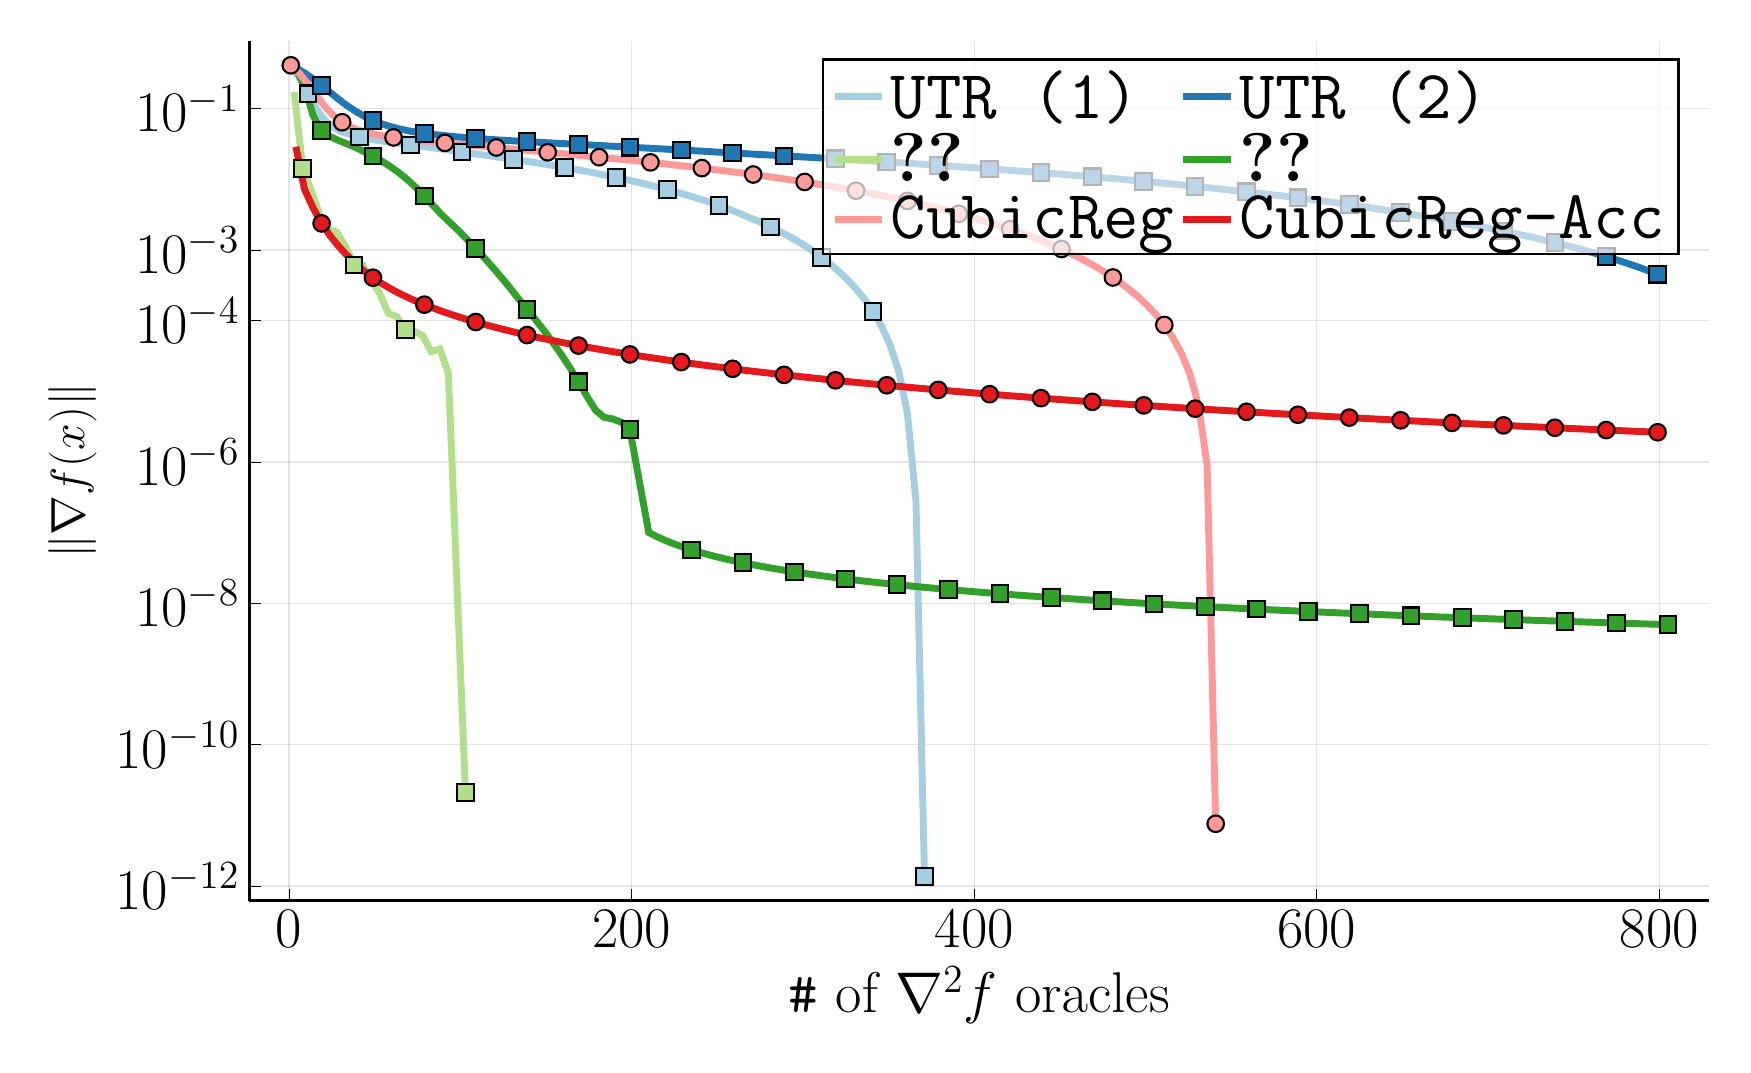
\begin{tikzpicture}[/tikz/background rectangle/.style={fill={rgb,1:red,1.0;green,1.0;blue,1.0}, fill opacity={1.0}, draw opacity={1.0}}, show background rectangle]
  \begin{axis}[point meta max={nan}, point meta min={nan}, legend cell align={left}, legend columns={2}, title={}, title style={at={{(0.5,1)}}, anchor={south}, font={{\fontsize{22 pt}{28.6 pt}\selectfont}}, color={rgb,1:red,0.0;green,0.0;blue,0.0}, draw opacity={1.0}, rotate={0.0}, align={center}}, legend style={color={rgb,1:red,0.0;green,0.0;blue,0.0}, draw opacity={1.0}, line width={1}, solid, fill={rgb,1:red,1.0;green,1.0;blue,1.0}, fill opacity={0.7}, text opacity={1.0}, font={{\fontsize{24 pt}{31.200000000000003 pt}\selectfont}}, text={rgb,1:red,0.0;green,0.0;blue,0.0}, cells={anchor={west}}, at={(0.98, 0.98)}, anchor={north east}}, axis background/.style={fill={rgb,1:red,1.0;green,1.0;blue,1.0}, opacity={1.0}}, anchor={north west}, xshift={1.0mm}, yshift={-1.0mm}, width={201.2mm}, height={125.0mm}, scaled x ticks={false}, xlabel={\texttt{\#} of $\nabla^2f$ oracles}, x tick style={color={rgb,1:red,0.0;green,0.0;blue,0.0}, opacity={1.0}}, x tick label style={color={rgb,1:red,0.0;green,0.0;blue,0.0}, opacity={1.0}, rotate={0}}, xlabel style={at={(ticklabel cs:0.5)}, anchor=near ticklabel, at={{(ticklabel cs:0.5)}}, anchor={near ticklabel}, font={{\fontsize{20 pt}{26.0 pt}\selectfont}}, color={rgb,1:red,0.0;green,0.0;blue,0.0}, draw opacity={1.0}, rotate={0.0}}, xmajorgrids={true}, xmin={-23.120000000000005}, xmax={829.12}, xticklabels={{$0$,$200$,$400$,$600$,$800$}}, xtick={{0.0,200.0,400.0,600.0,800.0}}, xtick align={inside}, xticklabel style={font={{\fontsize{20 pt}{26.0 pt}\selectfont}}, color={rgb,1:red,0.0;green,0.0;blue,0.0}, draw opacity={1.0}, rotate={0.0}}, x grid style={color={rgb,1:red,0.0;green,0.0;blue,0.0}, draw opacity={0.1}, line width={0.5}, solid}, axis x line*={left}, x axis line style={color={rgb,1:red,0.0;green,0.0;blue,0.0}, draw opacity={1.0}, line width={1}, solid}, scaled y ticks={false}, ylabel={$\|\nabla f(x)\|$}, y tick style={color={rgb,1:red,0.0;green,0.0;blue,0.0}, opacity={1.0}}, y tick label style={color={rgb,1:red,0.0;green,0.0;blue,0.0}, opacity={1.0}, rotate={0}}, ylabel style={at={(ticklabel cs:0.5)}, anchor=near ticklabel, at={{(ticklabel cs:0.5)}}, anchor={near ticklabel}, font={{\fontsize{17 pt}{22.1 pt}\selectfont}}, color={rgb,1:red,0.0;green,0.0;blue,0.0}, draw opacity={1.0}, rotate={0.0}}, ymode={log}, log basis y={10}, ymajorgrids={true}, ymin={6.220670277739033e-13}, ymax={0.9070952834409658}, yticklabels={{$10^{-12}$,$10^{-10}$,$10^{-8}$,$10^{-6}$,$10^{-4}$,$10^{-3}$,$10^{-1}$}}, ytick={{1.0e-12,1.0e-10,1.0e-8,1.0e-6,0.0001,0.001,0.1}}, ytick align={inside}, yticklabel style={font={{\fontsize{20 pt}{26.0 pt}\selectfont}}, color={rgb,1:red,0.0;green,0.0;blue,0.0}, draw opacity={1.0}, rotate={0.0}}, y grid style={color={rgb,1:red,0.0;green,0.0;blue,0.0}, draw opacity={0.1}, line width={0.5}, solid}, axis y line*={left}, y axis line style={color={rgb,1:red,0.0;green,0.0;blue,0.0}, draw opacity={1.0}, line width={1}, solid}, colorbar={false}]
    \addplot[color={rgb,1:red,0.651;green,0.808;blue,0.89}, name path={73}, draw opacity={1.0}, line width={2.5}, solid]
    table[row sep={\\}]
      {
        \\
        371.0  1.3743461118707057e-12  \\
        366.0  2.816615860294512e-7  \\
        361.0  4.948285384613171e-6  \\
        356.0  1.9045988579323584e-5  \\
        351.0  4.467498440373031e-5  \\
        346.0  8.29035836926752e-5  \\
        341.0  0.00013456450932675722  \\
        336.0  0.00020053647354741406  \\
        331.0  0.00028189119592813487  \\
        326.0  0.0003799408467759354  \\
        321.0  0.0004961140988605906  \\
        316.0  0.0006316404705364614  \\
        311.0  0.0007872036313181774  \\
        306.0  0.0009627966683117589  \\
        301.0  0.001157885240291366  \\
        296.0  0.0013718150100441922  \\
        291.0  0.0016042655623840112  \\
        286.0  0.001855527336237931  \\
        281.0  0.0021265083971393293  \\
        276.0  0.0024186335215047416  \\
        271.0  0.0027339256811991608  \\
        266.0  0.0030751265319052014  \\
        261.0  0.0034453372986904523  \\
        256.0  0.0038461274535546274  \\
        251.0  0.004271906662535761  \\
        246.0  0.004712164362273808  \\
        241.0  0.005164400120787778  \\
        236.0  0.005630994932427763  \\
        231.0  0.00611389628284721  \\
        226.0  0.006614487827420619  \\
        221.0  0.007134369751212193  \\
        216.0  0.0076752197339019015  \\
        211.0  0.008237154812092114  \\
        206.0  0.008818189249717077  \\
        201.0  0.009415965239988392  \\
        196.0  0.010028380465845638  \\
        191.0  0.010653428440476734  \\
        186.0  0.011290149487447228  \\
        181.0  0.011938821274344402  \\
        176.0  0.012600366645808036  \\
        171.0  0.013275749690088013  \\
        166.0  0.013965547602778022  \\
        161.0  0.014670312155616743  \\
        156.0  0.01539042244595522  \\
        151.0  0.016125042751803854  \\
        146.0  0.016873019570541898  \\
        141.0  0.017634246557140573  \\
        136.0  0.018409196458009525  \\
        131.0  0.01919816250754363  \\
        126.0  0.020001931206113686  \\
        121.0  0.020823966513334048  \\
        116.0  0.02167053332001754  \\
        111.0  0.02254692720076579  \\
        106.0  0.023456511472592166  \\
        101.0  0.02440497098379018  \\
        96.0  0.025393181676155327  \\
        91.0  0.026419931270457872  \\
        86.0  0.027457128141032412  \\
        81.0  0.02851446010469235  \\
        76.0  0.029619665008504305  \\
        71.0  0.030756034874515895  \\
        66.0  0.03190845418651997  \\
        61.0  0.03310741349255251  \\
        56.0  0.034407547661413865  \\
        51.0  0.035868215260032955  \\
        46.0  0.037593657538088396  \\
        41.0  0.03979223180773928  \\
        36.0  0.042667909008782985  \\
        31.0  0.04677873500672122  \\
        26.0  0.0541638329119768  \\
        21.0  0.06810523519460977  \\
        16.0  0.09852437521365984  \\
        11.0  0.1624204798714738  \\
        6.0  0.2740431199634093  \\
        1.0  0.4105763912045273  \\
      }
    ;
    \addlegendentry {$\texttt{UTR (1)}$}
    \addplot[color={rgb,1:red,0.8889;green,0.4356;blue,0.2781}, name path={74}, only marks, draw opacity={1.0}, line width={0}, solid, mark={square*}, mark size={3.0 pt}, mark repeat={1}, mark options={color={rgb,1:red,0.0;green,0.0;blue,0.0}, draw opacity={1.0}, fill={rgb,1:red,0.651;green,0.808;blue,0.89}, fill opacity={1.0}, line width={0.75}, rotate={0}, solid}, forget plot]
    table[row sep={\\}]
      {
        \\
        371.0  1.3743461118707057e-12  \\
        341.0  0.00013456450932675722  \\
        311.0  0.0007872036313181774  \\
        281.0  0.0021265083971393293  \\
        251.0  0.004271906662535761  \\
        221.0  0.007134369751212193  \\
        191.0  0.010653428440476734  \\
        161.0  0.014670312155616743  \\
        131.0  0.01919816250754363  \\
        101.0  0.02440497098379018  \\
        71.0  0.030756034874515895  \\
        41.0  0.03979223180773928  \\
        11.0  0.1624204798714738  \\
      }
    ;
    \addplot[color={rgb,1:red,0.122;green,0.471;blue,0.706}, name path={75}, draw opacity={1.0}, line width={2.5}, solid]
    table[row sep={\\}]
      {
        \\
        799.0  0.0004549423104272085  \\
        794.0  0.0005052694000551794  \\
        789.0  0.0005588038597993246  \\
        784.0  0.000615600055126194  \\
        779.0  0.0006756926785187809  \\
        774.0  0.000739095702635968  \\
        769.0  0.0008058029421640431  \\
        764.0  0.000875790183275068  \\
        759.0  0.0009490187404468095  \\
        754.0  0.0010254401768410714  \\
        749.0  0.0011050017954298  \\
        744.0  0.0011876524189800197  \\
        739.0  0.0012733479502845472  \\
        734.0  0.001362056232098568  \\
        729.0  0.0014537607989328967  \\
        724.0  0.0015484632323827041  \\
        719.0  0.0016461840023934062  \\
        714.0  0.0017469618953209688  \\
        709.0  0.0018508523883181266  \\
        704.0  0.001957925611389108  \\
        699.0  0.0020682647760333845  \\
        694.0  0.0021819659764776137  \\
        689.0  0.0022991398632334023  \\
        684.0  0.0024199147847141275  \\
        679.0  0.002544439949337117  \\
        674.0  0.0026728867075256416  \\
        669.0  0.002805446716766552  \\
        664.0  0.0029423271645550512  \\
        659.0  0.003083743974423836  \\
        654.0  0.0032299120614894088  \\
        649.0  0.0033810256676488682  \\
        644.0  0.0035372127030583044  \\
        639.0  0.0036984448080436476  \\
        634.0  0.0038644143825371335  \\
        629.0  0.0040344656310694615  \\
        624.0  0.004207711056210209  \\
        619.0  0.004383331221621482  \\
        614.0  0.004560836930614327  \\
        609.0  0.00474010462937748  \\
        604.0  0.004921241036024438  \\
        599.0  0.0051044355000846205  \\
        594.0  0.005289876248789827  \\
        589.0  0.00547772206411372  \\
        584.0  0.005668100587409691  \\
        579.0  0.005861115172511775  \\
        574.0  0.006056854064719013  \\
        569.0  0.006255400963691219  \\
        564.0  0.006456846202650598  \\
        559.0  0.0066612957666859415  \\
        554.0  0.006868873667596658  \\
        549.0  0.007079713438419977  \\
        544.0  0.007293937447176274  \\
        539.0  0.007511628142076705  \\
        534.0  0.007732801353449172  \\
        529.0  0.007957394316305837  \\
        524.0  0.008185276146783303  \\
        519.0  0.008416277063288544  \\
        514.0  0.008650222085770064  \\
        509.0  0.00888695318778222  \\
        504.0  0.009126332097920936  \\
        499.0  0.009368228213938738  \\
        494.0  0.009612504585216727  \\
        489.0  0.009859014715618206  \\
        484.0  0.010107614411989985  \\
        479.0  0.010358181981717746  \\
        474.0  0.010610634761957352  \\
        469.0  0.010864933809432575  \\
        464.0  0.011121077522331014  \\
        459.0  0.011379091318695203  \\
        454.0  0.011639019800698768  \\
        449.0  0.011900922303450077  \\
        444.0  0.012164868524135465  \\
        439.0  0.012430931477254215  \\
        434.0  0.012699178410831182  \\
        429.0  0.012969663224885478  \\
        424.0  0.013242424517361804  \\
        419.0  0.013517490964584296  \\
        414.0  0.013794891325039934  \\
        409.0  0.014074662871439938  \\
        404.0  0.01435685181101439  \\
        399.0  0.014641502121776343  \\
        394.0  0.014928634818032758  \\
        389.0  0.01521822778711516  \\
        384.0  0.01551021140845577  \\
        379.0  0.015804487478006533  \\
        374.0  0.016100961171974272  \\
        369.0  0.0163995664160238  \\
        364.0  0.016700274091146168  \\
        359.0  0.01700308711226224  \\
        354.0  0.017308030366622228  \\
        349.0  0.017615138699027907  \\
        344.0  0.017924444285931363  \\
        339.0  0.018235968001085633  \\
        334.0  0.018549719471943758  \\
        329.0  0.018865705097812237  \\
        324.0  0.019183943367937148  \\
        319.0  0.019504493322583305  \\
        314.0  0.019827492754023616  \\
        309.0  0.020153182892818967  \\
        304.0  0.02048190423686009  \\
        299.0  0.02081407208395254  \\
        294.0  0.02115014026210268  \\
        289.0  0.021490546482253403  \\
        284.0  0.021835637918000816  \\
        279.0  0.02218561912709437  \\
        274.0  0.022540606786473728  \\
        269.0  0.022900801052805064  \\
        264.0  0.023266610240566095  \\
        259.0  0.023638553712034556  \\
        254.0  0.02401697098757128  \\
        249.0  0.024401811921455793  \\
        244.0  0.024792848101501164  \\
        239.0  0.025190194920032317  \\
        234.0  0.025594382145812025  \\
        229.0  0.026005246279389507  \\
        224.0  0.02642044698396634  \\
        219.0  0.026836451749398083  \\
        214.0  0.027251907065022347  \\
        209.0  0.02766867393268195  \\
        204.0  0.028089872323718748  \\
        199.0  0.02851809377053373  \\
        194.0  0.02895466291429293  \\
        189.0  0.029399305317766588  \\
        184.0  0.029850221262941488  \\
        179.0  0.030304980378302114  \\
        174.0  0.030761838020729435  \\
        169.0  0.03122043653557724  \\
        164.0  0.031681833116351615  \\
        159.0  0.032148411393747904  \\
        154.0  0.03262324664065285  \\
        149.0  0.03310951349186461  \\
        144.0  0.033610990212603296  \\
        139.0  0.034132061615002526  \\
        134.0  0.03467683081379294  \\
        129.0  0.03524858431018801  \\
        124.0  0.03585126512355195  \\
        119.0  0.03649315224829594  \\
        114.0  0.03718754503713941  \\
        109.0  0.037949781384402186  \\
        104.0  0.03879319473912637  \\
        99.0  0.03973113692825133  \\
        94.0  0.040778025275733994  \\
        89.0  0.04193526428773949  \\
        84.0  0.043236704393297354  \\
        79.0  0.04475272859523595  \\
        74.0  0.0465871042710885  \\
        69.0  0.048945364688684254  \\
        64.0  0.05206544377717598  \\
        59.0  0.05596738270191759  \\
        54.0  0.06106070231511094  \\
        49.0  0.06799665042765445  \\
        44.0  0.07771856645386888  \\
        39.0  0.09145896634618357  \\
        34.0  0.10982518457992357  \\
        29.0  0.13550560986155616  \\
        24.0  0.1699413359092823  \\
        19.0  0.2135775615703503  \\
        14.0  0.2641219594248821  \\
        9.0  0.32063494631687095  \\
        4.0  0.3778815975026772  \\
      }
    ;
    \addlegendentry {$\texttt{UTR (2)}$}
    \addplot[color={rgb,1:red,0.7644;green,0.4441;blue,0.8243}, name path={76}, only marks, draw opacity={1.0}, line width={0}, solid, mark={square*}, mark size={3.0 pt}, mark repeat={1}, mark options={color={rgb,1:red,0.0;green,0.0;blue,0.0}, draw opacity={1.0}, fill={rgb,1:red,0.122;green,0.471;blue,0.706}, fill opacity={1.0}, line width={0.75}, rotate={0}, solid}, forget plot]
    table[row sep={\\}]
      {
        \\
        799.0  0.0004549423104272085  \\
        769.0  0.0008058029421640431  \\
        739.0  0.0012733479502845472  \\
        709.0  0.0018508523883181266  \\
        679.0  0.002544439949337117  \\
        649.0  0.0033810256676488682  \\
        619.0  0.004383331221621482  \\
        589.0  0.00547772206411372  \\
        559.0  0.0066612957666859415  \\
        529.0  0.007957394316305837  \\
        499.0  0.009368228213938738  \\
        469.0  0.010864933809432575  \\
        439.0  0.012430931477254215  \\
        409.0  0.014074662871439938  \\
        379.0  0.015804487478006533  \\
        349.0  0.017615138699027907  \\
        319.0  0.019504493322583305  \\
        289.0  0.021490546482253403  \\
        259.0  0.023638553712034556  \\
        229.0  0.026005246279389507  \\
        199.0  0.02851809377053373  \\
        169.0  0.03122043653557724  \\
        139.0  0.034132061615002526  \\
        109.0  0.037949781384402186  \\
        79.0  0.04475272859523595  \\
        49.0  0.06799665042765445  \\
        19.0  0.2135775615703503  \\
      }
    ;
    \addplot[color={rgb,1:red,0.698;green,0.875;blue,0.541}, name path={77}, draw opacity={1.0}, line width={2.5}, solid]
    table[row sep={\\}]
      {
        \\
        103.0  2.098741020764118e-11  \\
        93.0  1.818640345988927e-5  \\
        88.0  3.980223254093483e-5  \\
        83.0  3.653695681449291e-5  \\
        78.0  6.159431272842603e-5  \\
        73.0  7.091605881212623e-5  \\
        68.0  7.56531691345277e-5  \\
        63.0  0.00011387358476259845  \\
        58.0  0.00012655537004631868  \\
        53.0  0.00024168338593038267  \\
        48.0  0.00037257145767421275  \\
        43.0  0.0006136497614030745  \\
        38.0  0.0006122700136776876  \\
        33.0  0.0011099676215112824  \\
        28.0  0.0017784946444742975  \\
        23.0  0.001946794374839215  \\
        18.0  0.0031072754743086306  \\
        13.0  0.006903079946694326  \\
        8.0  0.014234121331684958  \\
        3.0  0.17209304917550544  \\
      }
    ;
    \addlegendentry {\Cref{alg.accelerated utr}}
    \addplot[color={rgb,1:red,0.0;green,0.6658;blue,0.681}, name path={78}, only marks, draw opacity={1.0}, line width={0}, solid, mark={square*}, mark size={3.0 pt}, mark repeat={1}, mark options={color={rgb,1:red,0.0;green,0.0;blue,0.0}, draw opacity={1.0}, fill={rgb,1:red,0.698;green,0.875;blue,0.541}, fill opacity={1.0}, line width={0.75}, rotate={0}, solid}, forget plot]
    table[row sep={\\}]
      {
        \\
        103.0  2.098741020764118e-11  \\
        68.0  7.56531691345277e-5  \\
        38.0  0.0006122700136776876  \\
        8.0  0.014234121331684958  \\
      }
    ;
    \addplot[color={rgb,1:red,0.2;green,0.627;blue,0.173}, name path={79}, draw opacity={1.0}, line width={2.5}, solid]
    table[row sep={\\}]
      {
        \\
        805.0  5.013298388309456e-9  \\
        800.0  5.055891112001024e-9  \\
        795.0  5.099172452222435e-9  \\
        790.0  5.1431592208848625e-9  \\
        785.0  5.187868779266421e-9  \\
        780.0  5.233319065945665e-9  \\
        775.0  5.2795286158589625e-9  \\
        770.0  5.326516589102905e-9  \\
        765.0  5.374302796150363e-9  \\
        760.0  5.422907723672543e-9  \\
        755.0  5.472352567060841e-9  \\
        750.0  5.522659261054562e-9  \\
        745.0  5.573850509208941e-9  \\
        740.0  5.625949818643816e-9  \\
        735.0  5.678981539885308e-9  \\
        730.0  5.7329709017424284e-9  \\
        725.0  5.78794404831109e-9  \\
        720.0  5.843928088811757e-9  \\
        715.0  5.900951135471878e-9  \\
        710.0  5.95904235133349e-9  \\
        705.0  6.018232006273225e-9  \\
        700.0  6.078551520510928e-9  \\
        695.0  6.140033525806002e-9  \\
        690.0  6.20271192316827e-9  \\
        685.0  6.26662194624037e-9  \\
        680.0  6.331800223404468e-9  \\
        675.0  6.39828485402207e-9  \\
        670.0  6.4661154748123655e-9  \\
        665.0  6.535333346497435e-9  \\
        660.0  6.605981433785147e-9  \\
        655.0  6.678104491578985e-9  \\
        650.0  6.751749165186998e-9  \\
        645.0  6.826964088450864e-9  \\
        640.0  6.9037999873173195e-9  \\
        635.0  6.982309800807632e-9  \\
        630.0  7.062548796154533e-9  \\
        625.0  7.144574704334873e-9  \\
        620.0  7.2284478532139275e-9  \\
        615.0  7.314231318872013e-9  \\
        610.0  7.40199108386414e-9  \\
        605.0  7.491796203858339e-9  \\
        600.0  7.583718992450872e-9  \\
        595.0  7.677835212881369e-9  \\
        590.0  7.774224287499572e-9  \\
        585.0  7.872969520713854e-9  \\
        580.0  7.974158339796195e-9  \\
        575.0  8.077882552724549e-9  \\
        570.0  8.184238626940926e-9  \\
        565.0  8.293327988334461e-9  \\
        560.0  8.405257342583704e-9  \\
        555.0  8.52013902581912e-9  \\
        550.0  8.638091380469249e-9  \\
        545.0  8.759239159855315e-9  \\
        540.0  8.883713971635357e-9  \\
        535.0  9.011654754789142e-9  \\
        530.0  9.143208295605823e-9  \\
        525.0  9.278529788453335e-9  \\
        520.0  9.417783453498292e-9  \\
        515.0  9.56114319468151e-9  \\
        510.0  9.708793329500098e-9  \\
        505.0  9.860929379180343e-9  \\
        500.0  1.0017805536490801e-8  \\
        495.0  1.0179729500410846e-8  \\
        490.0  1.0346853222018598e-8  \\
        485.0  1.0519430246327768e-8  \\
        480.0  1.0697730855393196e-8  \\
        475.0  1.0882043466300852e-8  \\
        470.0  1.1072676182691843e-8  \\
        465.0  1.126995849869204e-8  \\
        460.0  1.1474243187205305e-8  \\
        455.0  1.1685908395286258e-8  \\
        450.0  1.1905359962129174e-8  \\
        445.0  1.2133034001243637e-8  \\
        440.0  1.2369399777962024e-8  \\
        435.0  1.2614962914733409e-8  \\
        430.0  1.2870268984666135e-8  \\
        425.0  1.3135907532497474e-8  \\
        420.0  1.341251659295726e-8  \\
        415.0  1.3700787781303672e-8  \\
        410.0  1.4001472035893791e-8  \\
        405.0  1.4315386114191857e-8  \\
        400.0  1.4643419962768848e-8  \\
        395.0  1.498654510175321e-8  \\
        390.0  1.534582418834075e-8  \\
        385.0  1.5722421953296167e-8  \\
        380.0  1.6117617759454468e-8  \\
        375.0  1.6532820052922138e-8  \\
        370.0  1.6969583060614943e-8  \\
        365.0  1.7429626151016877e-8  \\
        360.0  1.791485635836514e-8  \\
        355.0  1.8427394702120867e-8  \\
        350.0  1.8969607063804862e-8  \\
        345.0  1.9544140563650337e-8  \\
        340.0  2.0153966628475275e-8  \\
        335.0  2.0802432222705753e-8  \\
        330.0  2.14933211057518e-8  \\
        325.0  2.2230927488937228e-8  \\
        320.0  2.302014512370757e-8  \\
        315.0  2.3866575718705495e-8  \\
        310.0  2.477666177691979e-8  \\
        305.0  2.5757850518653523e-8  \\
        300.0  2.681879771906305e-8  \\
        295.0  2.796962328810473e-8  \\
        290.0  2.922223459801677e-8  \\
        285.0  3.0590739493298196e-8  \\
        280.0  3.209197940652232e-8  \\
        275.0  3.374622546474457e-8  \\
        270.0  3.557809882778605e-8  \\
        265.0  3.7617804410303445e-8  \\
        260.0  3.990281003974647e-8  \\
        255.0  4.2480170847692556e-8  \\
        250.0  4.5409808217086695e-8  \\
        245.0  4.8769234673364286e-8  \\
        240.0  5.2660528496141845e-8  \\
        235.0  5.722091709462655e-8  \\
        230.0  6.263935636859665e-8  \\
        225.0  6.918348929883794e-8  \\
        220.0  7.724546290040992e-8  \\
        215.0  8.74240628834996e-8  \\
        210.0  1.0092124132559083e-7  \\
        199.0  2.8700956617809424e-6  \\
        194.0  3.664951017370367e-6  \\
        189.0  4.073074409210384e-6  \\
        184.0  4.285839746920904e-6  \\
        179.0  5.398969130982007e-6  \\
        174.0  8.4207636114691e-6  \\
        169.0  1.3658509769090145e-5  \\
        164.0  2.1624444589235125e-5  \\
        159.0  3.299088105063764e-5  \\
        154.0  4.91670111132932e-5  \\
        149.0  7.183165642153164e-5  \\
        144.0  0.00010277422177758469  \\
        139.0  0.00014492494695528716  \\
        134.0  0.00020339644792586486  \\
        129.0  0.00029128415049168785  \\
        124.0  0.0004085219238308563  \\
        119.0  0.0005652269445534201  \\
        114.0  0.0007750460710845608  \\
        109.0  0.0010518244543130488  \\
        104.0  0.0014131068932164389  \\
        99.0  0.0018759922666213816  \\
        94.0  0.0024420673934618044  \\
        89.0  0.003178780928146182  \\
        84.0  0.004289559592973995  \\
        79.0  0.005836848942404475  \\
        74.0  0.007691810635628199  \\
        69.0  0.009951306693698096  \\
        64.0  0.01249340988099112  \\
        59.0  0.01524344531619994  \\
        54.0  0.018197607951476492  \\
        49.0  0.021286895269537986  \\
        44.0  0.02458064311719458  \\
        39.0  0.028130643977417685  \\
        34.0  0.0317111437072504  \\
        29.0  0.03534756217619216  \\
        24.0  0.04023957104067095  \\
        19.0  0.04928631446074253  \\
        14.0  0.08029042908344206  \\
        9.0  0.20734711210891468  \\
        4.0  0.3642118599728355  \\
      }
    ;
    \addlegendentry {\Cref{alg.ms accelerated utr}}
    \addplot[color={rgb,1:red,0.777;green,0.5097;blue,0.1464}, name path={80}, only marks, draw opacity={1.0}, line width={0}, solid, mark={square*}, mark size={3.0 pt}, mark repeat={1}, mark options={color={rgb,1:red,0.0;green,0.0;blue,0.0}, draw opacity={1.0}, fill={rgb,1:red,0.2;green,0.627;blue,0.173}, fill opacity={1.0}, line width={0.75}, rotate={0}, solid}, forget plot]
    table[row sep={\\}]
      {
        \\
        805.0  5.013298388309456e-9  \\
        775.0  5.2795286158589625e-9  \\
        745.0  5.573850509208941e-9  \\
        715.0  5.900951135471878e-9  \\
        685.0  6.26662194624037e-9  \\
        655.0  6.678104491578985e-9  \\
        625.0  7.144574704334873e-9  \\
        595.0  7.677835212881369e-9  \\
        565.0  8.293327988334461e-9  \\
        535.0  9.011654754789142e-9  \\
        505.0  9.860929379180343e-9  \\
        475.0  1.0882043466300852e-8  \\
        445.0  1.2133034001243637e-8  \\
        415.0  1.3700787781303672e-8  \\
        385.0  1.5722421953296167e-8  \\
        355.0  1.8427394702120867e-8  \\
        325.0  2.2230927488937228e-8  \\
        295.0  2.796962328810473e-8  \\
        265.0  3.7617804410303445e-8  \\
        235.0  5.722091709462655e-8  \\
        199.0  2.8700956617809424e-6  \\
        169.0  1.3658509769090145e-5  \\
        139.0  0.00014492494695528716  \\
        109.0  0.0010518244543130488  \\
        79.0  0.005836848942404475  \\
        49.0  0.021286895269537986  \\
        19.0  0.04928631446074253  \\
      }
    ;
    \addplot[color={rgb,1:red,0.984;green,0.604;blue,0.6}, name path={81}, draw opacity={1.0}, line width={2.5}, solid]
    table[row sep={\\}]
      {
        \\
        541.0  7.627990671820975e-12  \\
        536.0  8.923361209230643e-7  \\
        531.0  6.335736572055521e-6  \\
        526.0  1.7451353597494044e-5  \\
        521.0  3.449983132145298e-5  \\
        516.0  5.764925860395412e-5  \\
        511.0  8.706135989144377e-5  \\
        506.0  0.00012291940745210697  \\
        501.0  0.00016544661258109178  \\
        496.0  0.00021492099784129802  \\
        491.0  0.00027168424294587746  \\
        486.0  0.00033613973990203407  \\
        481.0  0.0004087295491667874  \\
        476.0  0.0004898875656774298  \\
        471.0  0.0005799792613631999  \\
        466.0  0.0006792453329708092  \\
        461.0  0.0007877705717881985  \\
        456.0  0.0009054858743316826  \\
        451.0  0.0010322049843853104  \\
        446.0  0.0011676850964253316  \\
        441.0  0.0013117004200611999  \\
        436.0  0.001464109705537648  \\
        431.0  0.001624901705964751  \\
        426.0  0.0017942108086684023  \\
        421.0  0.001972304229305397  \\
        416.0  0.00215955892535523  \\
        411.0  0.0023564570801672827  \\
        406.0  0.00256361215296915  \\
        401.0  0.0027818002656660114  \\
        396.0  0.0030119434753032573  \\
        391.0  0.003255034745632851  \\
        386.0  0.003511953196156844  \\
        381.0  0.0037828567762775147  \\
        376.0  0.004065976163894137  \\
        371.0  0.004357576735545249  \\
        366.0  0.004654722728437627  \\
        361.0  0.004956945273415683  \\
        356.0  0.005265002936343681  \\
        351.0  0.005579692039909139  \\
        346.0  0.005901589847519717  \\
        341.0  0.006231125626900416  \\
        336.0  0.006568711128828932  \\
        331.0  0.006914854295562038  \\
        326.0  0.007270145345542633  \\
        321.0  0.007635025484389724  \\
        316.0  0.008009476750350327  \\
        311.0  0.008392953093531  \\
        306.0  0.00878467020191469  \\
        301.0  0.009183914653775991  \\
        296.0  0.009590060991549283  \\
        291.0  0.010002449938105982  \\
        286.0  0.010420454417469981  \\
        281.0  0.010843682270604766  \\
        276.0  0.011272049991335003  \\
        271.0  0.011705694941281706  \\
        266.0  0.012144884715875107  \\
        261.0  0.012589947679352793  \\
        256.0  0.01304117545747295  \\
        251.0  0.013498755590065782  \\
        246.0  0.01396282551010453  \\
        241.0  0.014433567930749885  \\
        236.0  0.014911166860965268  \\
        231.0  0.015395592423962297  \\
        226.0  0.015886495133611338  \\
        221.0  0.01638345571599217  \\
        216.0  0.01688627177302488  \\
        211.0  0.01739498210227902  \\
        206.0  0.017909740126926973  \\
        201.0  0.01843066887940717  \\
        196.0  0.01895782037861962  \\
        191.0  0.019491314072636042  \\
        186.0  0.020031677212761303  \\
        181.0  0.020580172359379954  \\
        176.0  0.021138690301676602  \\
        171.0  0.02170926223637624  \\
        166.0  0.022293284927410246  \\
        161.0  0.02289148983180096  \\
        156.0  0.023505402096701676  \\
        151.0  0.024137014667198683  \\
        146.0  0.024786386497129293  \\
        141.0  0.025453595728197317  \\
        136.0  0.026139137668842693  \\
        131.0  0.026833191904346083  \\
        126.0  0.02752733935918534  \\
        121.0  0.02823119091285473  \\
        116.0  0.02895585337406663  \\
        111.0  0.02970227022349014  \\
        106.0  0.030461549645445386  \\
        101.0  0.031226572700063515  \\
        96.0  0.032000530416936984  \\
        91.0  0.03279570771055317  \\
        86.0  0.033627736354686986  \\
        81.0  0.03451573135190978  \\
        76.0  0.03547693988688653  \\
        71.0  0.03653462694821893  \\
        66.0  0.03774450696490698  \\
        61.0  0.03917353539357163  \\
        56.0  0.040885304509010886  \\
        51.0  0.04293417391675164  \\
        46.0  0.045552243365555134  \\
        41.0  0.04933340856610233  \\
        36.0  0.0551796964807649  \\
        31.0  0.06421975258410438  \\
        26.0  0.07970946378194495  \\
        21.0  0.1067022567063918  \\
        16.0  0.15304143756621394  \\
        11.0  0.22519140381385  \\
        6.0  0.31597722361407216  \\
        1.0  0.4105763912045273  \\
      }
    ;
    \addlegendentry {$\texttt{CubicReg}$}
    \addplot[color={rgb,1:red,0.5585;green,0.5935;blue,0.1175}, name path={82}, only marks, draw opacity={1.0}, line width={0}, solid, mark={*}, mark size={3.0 pt}, mark repeat={1}, mark options={color={rgb,1:red,0.0;green,0.0;blue,0.0}, draw opacity={1.0}, fill={rgb,1:red,0.984;green,0.604;blue,0.6}, fill opacity={1.0}, line width={0.75}, rotate={0}, solid}, forget plot]
    table[row sep={\\}]
      {
        \\
        541.0  7.627990671820975e-12  \\
        511.0  8.706135989144377e-5  \\
        481.0  0.0004087295491667874  \\
        451.0  0.0010322049843853104  \\
        421.0  0.001972304229305397  \\
        391.0  0.003255034745632851  \\
        361.0  0.004956945273415683  \\
        331.0  0.006914854295562038  \\
        301.0  0.009183914653775991  \\
        271.0  0.011705694941281706  \\
        241.0  0.014433567930749885  \\
        211.0  0.01739498210227902  \\
        181.0  0.020580172359379954  \\
        151.0  0.024137014667198683  \\
        121.0  0.02823119091285473  \\
        91.0  0.03279570771055317  \\
        61.0  0.03917353539357163  \\
        31.0  0.06421975258410438  \\
        1.0  0.4105763912045273  \\
      }
    ;
    \addplot[color={rgb,1:red,0.89;green,0.102;blue,0.11}, name path={83}, draw opacity={1.0}, line width={2.5}, solid]
    table[row sep={\\}]
      {
        \\
        799.0  2.6407667917528464e-6  \\
        794.0  2.6720703108208028e-6  \\
        789.0  2.703938191197356e-6  \\
        784.0  2.7364318070854445e-6  \\
        779.0  2.769465218367762e-6  \\
        774.0  2.8031509645516574e-6  \\
        769.0  2.8374138202534575e-6  \\
        764.0  2.87235729946256e-6  \\
        759.0  2.907904700670035e-6  \\
        754.0  2.944175204855662e-6  \\
        749.0  2.981132505071613e-6  \\
        744.0  3.0187495906110005e-6  \\
        739.0  3.057138723255576e-6  \\
        734.0  3.0962631191797993e-6  \\
        729.0  3.1360953401688276e-6  \\
        724.0  3.176766545789622e-6  \\
        719.0  3.218238342134766e-6  \\
        714.0  3.260530691996674e-6  \\
        709.0  3.3036626779505614e-6  \\
        704.0  3.3476678453480516e-6  \\
        699.0  3.3925672971482263e-6  \\
        694.0  3.438382801944001e-6  \\
        689.0  3.485136820135794e-6  \\
        684.0  3.532852531171885e-6  \\
        679.0  3.5815676982236778e-6  \\
        674.0  3.631294064080913e-6  \\
        669.0  3.682083964484003e-6  \\
        664.0  3.7340043920672345e-6  \\
        659.0  3.7869917184062346e-6  \\
        654.0  3.8411117828151685e-6  \\
        649.0  3.896465214056841e-6  \\
        644.0  3.952972384306782e-6  \\
        639.0  4.010791397790673e-6  \\
        634.0  4.069827602104435e-6  \\
        629.0  4.130275653645137e-6  \\
        624.0  4.192083460286347e-6  \\
        619.0  4.255289728769971e-6  \\
        614.0  4.319884507679916e-6  \\
        609.0  4.386047687407832e-6  \\
        604.0  4.45375955222175e-6  \\
        599.0  4.523063638282593e-6  \\
        594.0  4.594005081554112e-6  \\
        589.0  4.666714696594051e-6  \\
        584.0  4.741107288529849e-6  \\
        579.0  4.8173147230880344e-6  \\
        574.0  4.895463043307317e-6  \\
        569.0  4.9754499911363685e-6  \\
        564.0  5.057524471501258e-6  \\
        559.0  5.1415688163685165e-6  \\
        554.0  5.227827488088972e-6  \\
        549.0  5.3162915687174176e-6  \\
        544.0  5.407046191646389e-6  \\
        539.0  5.500162743499408e-6  \\
        534.0  5.5957155225968565e-6  \\
        529.0  5.693816757482094e-6  \\
        524.0  5.794618183319844e-6  \\
        519.0  5.898066132316469e-6  \\
        514.0  6.004409024396089e-6  \\
        509.0  6.113705978417442e-6  \\
        504.0  6.226055268322993e-6  \\
        499.0  6.341559446286468e-6  \\
        494.0  6.460325575484377e-6  \\
        489.0  6.582465478330024e-6  \\
        484.0  6.708217632473461e-6  \\
        479.0  6.8375588666361065e-6  \\
        474.0  6.970807829528541e-6  \\
        469.0  7.108017212694569e-6  \\
        464.0  7.249369338509971e-6  \\
        459.0  7.395017637593879e-6  \\
        454.0  7.545249315188792e-6  \\
        449.0  7.700147506907941e-6  \\
        444.0  7.85978706411146e-6  \\
        439.0  8.024750784391977e-6  \\
        434.0  8.194857334063788e-6  \\
        429.0  8.370475868937562e-6  \\
        424.0  8.55201416179822e-6  \\
        419.0  8.73955775613607e-6  \\
        414.0  8.93354975195739e-6  \\
        409.0  9.133983348813902e-6  \\
        404.0  9.34144583895093e-6  \\
        399.0  9.556302816285959e-6  \\
        394.0  9.778532154640952e-6  \\
        389.0  1.0008862032013274e-5  \\
        384.0  1.024749197398294e-5  \\
        379.0  1.0495023102441403e-5  \\
        374.0  1.075171133298355e-5  \\
        369.0  1.1018023793273445e-5  \\
        364.0  1.1294641562512074e-5  \\
        359.0  1.1581894883112336e-5  \\
        354.0  1.1880547257014056e-5  \\
        349.0  1.2191005585963316e-5  \\
        344.0  1.2514116040290684e-5  \\
        339.0  1.2850379393204775e-5  \\
        334.0  1.3200667915135743e-5  \\
        329.0  1.3565914499953415e-5  \\
        324.0  1.3946639867247547e-5  \\
        319.0  1.434400751299852e-5  \\
        314.0  1.475898898506949e-5  \\
        309.0  1.5192446191086484e-5  \\
        304.0  1.5645702908279203e-5  \\
        299.0  1.6119993013530917e-5  \\
        294.0  1.66166992059328e-5  \\
        289.0  1.713721296221024e-5  \\
        284.0  1.7683096809248013e-5  \\
        279.0  1.8256018909276057e-5  \\
        274.0  1.8858117810789253e-5  \\
        269.0  1.9490786722105743e-5  \\
        264.0  2.0156788289498565e-5  \\
        259.0  2.0858587190420906e-5  \\
        254.0  2.1597988534404704e-5  \\
        249.0  2.2378847355143424e-5  \\
        244.0  2.3204000504441378e-5  \\
        239.0  2.4076463558317455e-5  \\
        234.0  2.5000340517246996e-5  \\
        229.0  2.5980184687544607e-5  \\
        224.0  2.7020188729009948e-5  \\
        219.0  2.8125854450615154e-5  \\
        214.0  2.930233853063135e-5  \\
        209.0  3.0556835680801086e-5  \\
        204.0  3.18958859928151e-5  \\
        199.0  3.3327294900893616e-5  \\
        194.0  3.486091751335533e-5  \\
        189.0  3.650609380351682e-5  \\
        184.0  3.827459215610779e-5  \\
        179.0  4.0179015052813836e-5  \\
        174.0  4.2234364075182304e-5  \\
        169.0  4.445704668696858e-5  \\
        164.0  4.6867128326739606e-5  \\
        159.0  4.948551981943703e-5  \\
        154.0  5.233947666017601e-5  \\
        149.0  5.545711090881435e-5  \\
        144.0  5.88746447291105e-5  \\
        139.0  6.263179442066231e-5  \\
        134.0  6.677702960617849e-5  \\
        129.0  7.136901896149127e-5  \\
        124.0  7.647496079356075e-5  \\
        119.0  8.217947834152046e-5  \\
        114.0  8.858210240083259e-5  \\
        109.0  9.580708438078334e-5  \\
        104.0  0.0001040101871921064  \\
        99.0  0.0001133830737240639  \\
        94.0  0.00012417379233847317  \\
        89.0  0.00013669834260521567  \\
        84.0  0.000151369946760821  \\
        79.0  0.00016874682255045632  \\
        74.0  0.00018958208817307593  \\
        69.0  0.00021492872633345193  \\
        64.0  0.00024630732077365034  \\
        59.0  0.0002859727178786962  \\
        54.0  0.0003373935327519961  \\
        49.0  0.0004060383088867796  \\
        44.0  0.0005006326784383845  \\
        39.0  0.0006350578529793227  \\
        34.0  0.000831462449211671  \\
        29.0  0.0011266858711917588  \\
        24.0  0.0015895452760233892  \\
        19.0  0.0023787005091537978  \\
        14.0  0.003963675876891177  \\
        9.0  0.007247835550972409  \\
        4.0  0.02892033162154882  \\
      }
    ;
    \addlegendentry {$\texttt{CubicReg-Acc}$}
    \addplot[color={rgb,1:red,0.6097;green,0.4992;blue,0.9118}, name path={84}, only marks, draw opacity={1.0}, line width={0}, solid, mark={*}, mark size={3.0 pt}, mark repeat={1}, mark options={color={rgb,1:red,0.0;green,0.0;blue,0.0}, draw opacity={1.0}, fill={rgb,1:red,0.89;green,0.102;blue,0.11}, fill opacity={1.0}, line width={0.75}, rotate={0}, solid}, forget plot]
    table[row sep={\\}]
      {
        \\
        799.0  2.6407667917528464e-6  \\
        769.0  2.8374138202534575e-6  \\
        739.0  3.057138723255576e-6  \\
        709.0  3.3036626779505614e-6  \\
        679.0  3.5815676982236778e-6  \\
        649.0  3.896465214056841e-6  \\
        619.0  4.255289728769971e-6  \\
        589.0  4.666714696594051e-6  \\
        559.0  5.1415688163685165e-6  \\
        529.0  5.693816757482094e-6  \\
        499.0  6.341559446286468e-6  \\
        469.0  7.108017212694569e-6  \\
        439.0  8.024750784391977e-6  \\
        409.0  9.133983348813902e-6  \\
        379.0  1.0495023102441403e-5  \\
        349.0  1.2191005585963316e-5  \\
        319.0  1.434400751299852e-5  \\
        289.0  1.713721296221024e-5  \\
        259.0  2.0858587190420906e-5  \\
        229.0  2.5980184687544607e-5  \\
        199.0  3.3327294900893616e-5  \\
        169.0  4.445704668696858e-5  \\
        139.0  6.263179442066231e-5  \\
        109.0  9.580708438078334e-5  \\
        79.0  0.00016874682255045632  \\
        49.0  0.0004060383088867796  \\
        19.0  0.0023787005091537978  \\
      }
    ;
  \end{axis}
\end{tikzpicture}
}
    }

    % \subcaptionbox{Runtime (seconds)}{
    %     
\includegraphics[width=0.47\columnwidth]{icml2025/figs/fx-softmax-t.pdf}
    % }
    \caption{Logistic regression using the LIBSVM datasets}\label{fig.logistic regression}
    \normalsize
\end{figure}

The subproblems arising in \arc{} and \arca{} are solved by a 1-D line-search strategy according to \cite{nesterov_lectures_2018}. Similarly, \ref{eq.newTR} (in \utr{}, \atr{} and \atrms{}) is solved by searching the dual variable. All methods use exact Hessian evaluation and Cholesky factorization to solve the linear systems.
Since these SOMs use different subproblems, and theoretically, the complexity rates to solve them vary from $O\left(\log\left(1/\epsilon\right)\right)$ (for subproblems in a cubic regularized method \cite{nesterov2006cubic}) to $O\left(\log\log\left(1/\epsilon\right)\right)$ (for \ref{eq.newTR} \cite{yenewcomplexityresult1991,vavasisProvingPolynomialtimeSphereconstrained1990}),
we report the number of Hessian evaluations needed in the method. In \Cref{fig.logistic regression}, the performance of the SOMs on some LIBSVM datasets\footnote{For details, see \url{https://www.csie.ntu.edu.tw/cjlin/libsvmtools/datasets/}} is reported.

We could have several observations. Firstly, for non-accelerated methods, a trend of local superlinear convergence can be observed in \utr{}~\texttt{(1)}, \utr{}~\texttt{(2)} and \arc{}. We could conclude that these three methods are comparable.
Secondly, in the beginning of the iterations, all accelerated methods, including \atr{}, \atrms{}, and \arca{}, converge faster than the non-accelerated methods (e.g., \utr{}~\texttt{(1)}, \utr{}~\texttt{(2)}, \arc{}). This confirms the effectiveness of the global acceleration. 

Secondly, the global convergence does come at the expense of local superlinear convergence.
Notably, \atr{} is the only accelerated method that has the local rate of superlinear convergence because of the diving track.
Both \atrms{} and \arca{} converge sublinearly in the local regime, in which \atrms{} is slightly better because of its superior $\tilde O(\epsilon^{-2/7})$ non-asymptotic performance. These results are in accordance with what is predicted in the convergence analysis.

\newpage
\addcontentsline{toc}{section}{References}

\bibliographystyle{plainnat}
\bibliography{arxiv_version/ref_arxiv}
\newpage
\appendix
\section{Technical proofs in~\Cref{sec.priliminary}}\label{sec.proof pre}
\subsection*{Proof to~\Cref{lem.bound next gradient}}
\begin{proof}
    From \eqref{eq.second-order exp}, we have
    \begin{equation*}
        \|\nabla f(x+d)- \nabla f(x) -\nabla ^2 f(x) d\| \leq \frac{M}{2}\|d\|^2.
    \end{equation*}
    By \eqref{eq.second-order update} and the above, we have
    \begin{equation}\label{eq.bounded by squared step}
        \|\nabla f(x+d)+\mu d\| \leq \frac{M}{2}\|d\|^2.
    \end{equation}
    Applying the triangle inequality and rearranging items, we can derive \eqref{eq.bound next gradient}.
\end{proof}
\subsection*{Proof to~\Cref{lem.inner product g and d}}
\begin{proof}
    Squaring both sides of \eqref{eq.bounded by squared step} and rearranging items, we have
    \begin{equation*}
        \begin{aligned}
            2\mu \langle \nabla f(x+d),-d \rangle & \geq \|\nabla f(x+d)\|^2 +\mu^2 \|d\|^2 -\frac{M}{4}\|d\|^4 \\
                                                  & \geq \|\nabla f(x+d)\|^2 +\frac{3}{4}\mu^2 \|d\|^2.
        \end{aligned}
    \end{equation*}
    The second line is due to $\mu\geq M\|d\|$, dividing both sides by $2\mu$ gives \eqref{eq.inner product g d}. Further, when $\mu \leq 2M\|d\|$, the above gives
    \begin{equation*}
        4M\|d\| \langle \nabla f(x+d),-d \rangle \geq \|f(x+d)\|^2 +\frac{3}{4} M^2 \|d\|^4,
    \end{equation*}
    which yields
    \begin{equation*}
        \langle \nabla f(x+d),-d \rangle \geq \frac{\|f(x+d)\|^2}{4M\|d\|}+\frac{3}{16}M\|d\|^3.
    \end{equation*}
    Consider an auxiliary function $h(t) = \frac{\|f(x+d)\|^2}{4Mt}+\frac{3}{16}Mt^3$ where $t\geq 0$, taking derivatives gives $h(t)$ achieves its minimum at $t^*= \frac{\sqrt{2}\|\nabla f(x+d)\|^{1/2}}{\sqrt{3M}}$, plugging $t^*$ back gives \eqref{eq.inner product g d advanced}.
\end{proof}
\section{Technical proofs in~\Cref{sec.first variant}}\label{sec.proof variant 1}
\subsection*{Proof to \Cref{lem.bound target interval}}
To prove \Cref{lem.bound target interval}, we first introduce the following lemma, which discusses the property of the auxiliary function $g_y(\mu)$.
\begin{lemma}
    \label{lem.property g}
    For any $y\in \mathbb{R}^n$, $g_y(\mu)$ is continuously differentiable and monotonically increasing for $\mu \in \left (0,+\infty\right ]$ and
    \begin{equation}
        \label{eq.derivative}
        g_y'(\mu) = \frac{1}{\|\left (\nabla ^2 f(y)+\mu I \right)^{-1}\nabla f(y)\|}+\frac{\mu}{\|\left (\nabla ^2 f(y)+\mu I \right)^{-1}\nabla f(y)\|^3}\sum_{i=1}^n\frac{\beta_i^2}{\left (\lambda_i+\mu\right )^3},
    \end{equation}
    and it is bounded both below and above
    \begin{equation}
        \label{eq.derivative bound}
        0< g_y'(\mu) \leq \frac{2}{\|\left (\nabla ^2 f(y)+\mu I \right)^{-1}\nabla f(y)\|}.
    \end{equation}
    Where $\lambda_i$ is the $i$-th eigenvalue of $\nabla ^2 f(y)$, $\beta_i = \nabla f(y)^T v_i$, $v_i$ denotes the eigenvector corresponding to $\lambda_i$.
\end{lemma}
\begin{proof}
    Since $\nabla^2 f(y)+\mu I \succ 0$ for $\mu>0$, we can apply eigen decomposition to it, then
    \begin{equation*}
        \|\left (\nabla ^2 f(y)+\mu I \right)^{-1}\nabla f(y)\|=\sqrt{\sum_{i=1}^n \frac{\beta_i^2}{\left (\lambda_i+\mu\right )^2}}, \ g_y(\mu) = \frac{\mu}{\sqrt{\sum_{i=1}^n \frac{\beta_i^2}{\left (\lambda_i+\mu\right )^2}}}.
    \end{equation*}
    Obviously $g_y(\mu)$ is increasing in $\mu \in \left (0,+\infty\right ]$. Also, through some basic calculations, we have
    \begin{equation*}
        \begin{aligned}
            g_y'(\mu) & = \frac{1}{\sqrt{\sum_{i=1}^n \frac{\beta_i^2}{\left (\lambda_i+\mu\right )^2}}}+\mu \frac{1}{\left ( \sum_{i=1}^n \frac{\beta_i^2}{\left (\lambda_i+\mu\right )^2}\right )^{3/2}}\sum_{i=1}^n\frac{\beta_i^2}{\left (\lambda_i+\mu\right )^3} \\
                      & = \frac{1}{\|\left (\nabla ^2 f(y)+\mu I \right)^{-1}\nabla f(y)\|}+\frac{\mu}{\|\left (\nabla ^2 f(y)+\mu I \right)^{-1}\nabla f(y)\|^3}\sum_{i=1}^n\frac{\beta_i^2}{\left (\lambda_i+\mu\right )^3}                                          \\
                      & \leq \frac{1}{\|\left (\nabla ^2 f(y)+\mu I \right)^{-1}\nabla f(y)\|}+\frac{\mu}{\|\left (\nabla ^2 f(y)+\mu I \right)^{-1}\nabla f(y)\|^3}\sum_{i=1}^n\frac{\beta_i^2}{\mu\left (\lambda_i+\mu\right )^2}                                    \\
                      & =  \frac{2}{\|\left (\nabla ^2 f(y)+\mu I \right)^{-1}\nabla f(y)\|}.
        \end{aligned}
    \end{equation*}
    The inequality is because of $\lambda_i \geq 0$ for $i=1,\ldots,n$.
\end{proof}

Now we are ready to formally prove \Cref{lem.bound target interval}.
\begin{proof}
    From the continuity and monotonicity of $g_y(\mu)$, we know there exists interval $[\mu_l,\mu_u]$ with \eqref{eq.target interval bracketing points} and
    \begin{equation*}
        M\leq g_y(\mu)\leq 2M
    \end{equation*}
    for all $\mu$ in this interval~(intermediate value theorem).

    Now we show that the length of the target interval for $\mu$ is bounded below; By the mean value theorem, there exists $\xi\in \left [\mu_l,\mu_u\right]$, such that
    \begin{equation*}
        M=g_y(\mu_u)-g_y(\mu_l) = g_y'(\xi)(\mu_u-\mu_l),
    \end{equation*}
    combine the above with \eqref{eq.derivative bound} and \eqref{eq.target interval bracketing points} we have
    \begin{equation*}
        \begin{aligned}
            \mu_u-\mu_l & =  \frac{1}{g_y'(\xi)}\left(g_y(\mu_u)-g_y(\mu_l)\right)                    \\
                        & \geq \frac{M\|\left (\nabla ^2 f(y)+\xi I \right )^{-1}\nabla f(y)\|}{2}    \\
                        & \geq \frac{M\|\left (\nabla ^2 f(y)+\mu_u I \right )^{-1}\nabla f(y)\|}{2}.
        \end{aligned}
    \end{equation*}
    The third line is because of $\mu_+ >\xi$.
\end{proof}
\subsection*{Proof to \Cref{lem.bound initial interval}}
\begin{proof}
    Denote the target interval for $r$ as $[r_l,r_u]$ and
    \begin{equation*}
        r_y(\mu)=\|\left (\nabla^2 f(y)+\mu I\right)^{-1}\nabla f(y)\|,
    \end{equation*}
    we have
    \begin{equation*}
        r_l = r_y(\mu_u), \ r_u=r_y(\mu_l).
    \end{equation*}
    The bisection terminates whenever $r\in[r_l,r_u]$. Note that by the mechanism of bisection, the oracle complexity is bounded by
    \begin{equation*}
        O\left(\log\frac{r_+-r_-}{r_u-r_l}\right)\leq O\left(\log\frac{r_+}{r_u-r_l}\right) \leq O\left(\log\frac{r_+}{r_y(\mu_l)-r_y(\mu_u)}\right).
    \end{equation*}
    For $r_y(\mu_l)-r_y(\mu_u)$, we have
    \begin{equation*}
        \begin{aligned}
            r_y(\mu_l)-r_y(\mu_u) & =r_y'(\xi)(\mu_l-\mu_u), \ \xi\in[\mu_l,\mu_u]                                                                                         \\
                                  & =\frac{\sum_{i=1}^n \frac{\beta_i^2}{(\lambda_i+\xi)^3}}{\left\|\left(\nabla^2 f(y)+\xi I\right)^{-1}\nabla f(y)\right\|}(\mu_u-\mu_l) \\
                                  & \geq \frac{1}{\kappa_H+\mu_u} \left\|\left(\nabla^2 f(y)+\xi I\right)^{-1}\nabla f(y)\right\|(\mu_u-\mu_l)                             \\
                                  & \geq \frac{1}{\kappa_H+\mu_u} \left\|\left(\nabla^2 f(y)+\mu_u I\right)^{-1}\nabla f(y)\right\|^2                                      \\
                                  & \geq \frac{\|\nabla f(y)\|^2}{(\kappa_H+\mu_u)^3}.
        \end{aligned}
    \end{equation*}
    In the above equations, the second line is derived by taking derivative of $r_y(\mu)$, which is similar to the analysis in \Cref{lem.property g}. The third line is from Assumption~\ref{assm.bounded hessian}. The fourth line is from \eqref{eq.bound target interval}. Therefore, we have
    \begin{equation*}
        \begin{aligned}
            O\left(\log\frac{r_+}{r_y(\mu_l)-r_y(\mu_u)}\right) & \leq O\left(\log\frac{r_+(\kappa_H+\mu_u)^3}{\|\nabla f(y)\|^2}\right)                                                                                \\
                                                                & \leq O\left(\log\frac{\|\nabla f(y)\|(\kappa_H+\mu_u)^3}{M\|d_+\|\|\nabla f(y)\|^2}\right)                                                            \\
                                                                & = O\left(\log\frac{(\kappa_H+\mu_u)^3}{M\|d_+\|\|\nabla f(y)\|}\right)                                                                                \\
                                                                & \leq O\left(\log\frac{(\kappa_H+\mu_+)^3}{8M\|d_+\|^2}\right)                                                                                         \\
                                                                & \leq  \max \left\{O\left(\log\frac{(\kappa_H+\mu_+)^3}{8\epsilon}\right),O\left(\log\frac{4\kappa_H^2(\kappa_H+\mu_+)^3}{8M\epsilon^2}\right)\right\} \\
                                                                & = O\left(\log\frac{\kappa_H+\mu_+}{\epsilon}\right).
        \end{aligned}
    \end{equation*}
    In the above, the second line is from
    $$r_+ = \left\|\left(\nabla^2 f(y)+M\|d_+\|I\right)^{-1} \nabla f(y)\right\| \leq \frac{\|\nabla f(y)\|}{M\|d_+\|}.$$
    The fourth line is from $\mu_u \leq \mu_+$ and
    $$
        \frac{\sqrt{2M}}{2}\|\nabla f(y)\| =\mu_+ \geq 2M\|d_+\|.
    $$
    The last line is from the proposition of the logarithmic function.
\end{proof}
\subsection*{Proof to \Cref{lem.enter region}}
\begin{proof}
    We first examine the distance between $y_k$ and $x^*$:
    \begin{equation*}
        \begin{aligned}
            \|y_k-x^*\| & \leq \|x_k-x^*\|+\|x_k-y_k\|                                                \\
                        & =\|x_k-x^*\|+\frac{a_k}{A_k+a_k}\|x_k-v_k\|                                 \\
                        & = \|x_k-x^*\|+\frac{3}{k+3}\|x_k-v_k\|                                      \\
                        & =\|x_k-x^*\|+\frac{3}{k+3}\|x_k-x^*+x^*-v_k\|                               \\
                        & \leq (1+\frac{3}{k+3})\|x_k-x^*\|+\frac{3}{k+3}\|x^*\|+\frac{3}{k+3}\|v_k\|
        \end{aligned}
    \end{equation*}
    In the above, the first line is from the triangle inequality. The second line is from the definition of $y_k$. The last line is from the triangle inequality.

    For the first term $\|x_k-x^*\|$, we first show that when $k\geq \frac{3^{4/3}M\|x_0-x^*\|}{2\nu}$, we have $x_k\in \mathcal{LQ}_p$~(see~\eqref{eq.local quadratic region}): for any $x\in\mathbb{R}^n$ with $\|x-x^*\| = \frac{2\nu}{3M}$, which means $x$ lies on the boundary of $\mathcal{LQ}_p$,
    we have
    \begin{equation*}
        \begin{aligned}
            f(x) & \geq f^* + \langle\nabla f(x^*),x-x^*\rangle +\frac{1}{2}(x-x^*)^T \nabla ^2 f(\chi x+(1-\chi)x^*)(x-x^*) \\
                 & \geq f^*+\frac{\nu}{6}\|x-x^*\|^2                                                                         \\
                 & =f^*+\frac{2\nu^3}{27M^2},
        \end{aligned}
    \end{equation*}
    where $\chi\in [0,1]$, and the second line is from \eqref{eq.psd region}. Therefore, for any $x\in\mathbb{R}^n$ with $\|x-x^*\| >\frac{2\nu}{3M}$, we also have
    \begin{equation*}
        f(x)\geq f^*+\frac{2\nu^3}{27M^2}
    \end{equation*}
    due to the convexity of $f$. When $k\geq \frac{3^{4/3}M\|x_0-x^*\|}{2\nu}$, we have
    \begin{equation*}
        f(x_k)-f^*< \frac{2\nu^3}{27M^2}.
    \end{equation*}
    Therefore, $x_k\in\mathcal{LQ}_p$.

    Moreover, we have $\nabla^2 f(x) >\frac{\nu}{3}I$ for all $x$ between $x_k$ and $x^*$, which further implies:
    \begin{equation*}
        \frac{\nu}{6}\|x_k-x^*\|^2 \leq f(x_k)-f^* \leq \frac{\phi_0(x^*)}{A_k}=\frac{3M\|x_0-x^*\|^3}{4 k(k+1)(k+2)}.
    \end{equation*}
    For the term $\|v_k\|$, we have
    \begin{equation*}
        \begin{aligned}
            \|v_k\| & =\|v_0-\sqrt{\frac{8}{3M\|s_{k}\|}}s_k\|       \\
                    & \leq \|v_0\|+\sqrt{\frac{8}{3M}}\|s_k\|^{1/2}.
        \end{aligned}
    \end{equation*}
    Since $\frac{1}{2\kappa_H}\|\nabla f(x_k)\|^2 \leq f(x_k)-f^* \leq \frac{3M\|x_0-x^*\|^3}{4 k(k+1)(k+2)}$, we have
    \begin{equation*}
        \|\nabla f(x_k)\|\leq \sqrt{\frac{3\kappa_H M\|x_0-x^*\|^3}{2 k(k+1)(k+2)}}.
    \end{equation*}
    Note
    \begin{equation*}
        \begin{aligned}
            \|s_k\| & =\|\sum_{i=1}^k\frac{i(i+1)}{2}\nabla f(x_i)\|                                         \\
                    & \leq \sum_{i=1}^k \frac{i(i+1)}{2}\|\nabla f(x_i)\|                                    \\
                    & \leq \sum_{i=1}^k\frac{i(i+1)}{2}\sqrt{\frac{3\kappa_H M\|x_0-x^*\|^3}{2 i(i+1)(i+2)}} \\
                    & \leq \sqrt{\frac{3\kappa_H M\|x_0-x^*\|^3}{2}}\sum_{i=1}^k\frac{\sqrt{i}}{2}           \\
                    & \leq \sqrt{\frac{3\kappa_H M\|x_0-x^*\|^3}{2}}\int_0^k \frac{\sqrt{t}}{2}dt            \\
                    & =\sqrt{\frac{\kappa_H M\|x_0-x^*\|^3}{6}}k^{3/2}.
        \end{aligned}
    \end{equation*}
    Therefore, $\|v_k\|\leq \|v_0\|+\frac{4\kappa_H^{1/4}\|x_0-x^*\|^{3/4}}{6^{3/4}M^{1/4}}k^{3/4}$. As a result,
    \begin{equation}
        \label{eq.bound yk}
        \begin{aligned}
            \|y_k-x^*\|\leq & (1+\frac{3}{k+3})\|x_k-x^*\|+\frac{3}{k+3}\|x^*\|                                      \\
                            & +\frac{3}{k+3}\|v_0\|+\frac{12\kappa_H^{1/4}\|x_0-x^*\|^{3/4}}{6^{3/4}M^{1/4}}k^{-1/4} \\
            \leq            & (1+\frac{3}{k+3})\sqrt{\frac{9M\|x_0-x^*\|^3}{2\nu k(k+1)(k+2)}}+\frac{3}{k+3}\|x^*\|  \\&
            +\frac{3}{k+3}\|v_0\|+\frac{12\kappa_H^{1/4}\|x_0-x^*\|^{3/4}}{6^{3/4}M^{1/4}}k^{-1/4}.
        \end{aligned}
    \end{equation}
    For the gradient norm, we have
    \begin{equation*}
        \|\nabla f(y_k)\| = \|\nabla f(y_k)-\nabla f(x^*)\|\leq \kappa_H\|y_k-x^*\|.
    \end{equation*}
    Therefore, when
    \begin{equation}\label{eq.quadratic region guarantee}
        \|y_k-x^*\|\leq \min\{\frac{2\nu}{3M},\frac{2\nu}{9\kappa_HM}\},
    \end{equation}
    we have $y_k\in\mathcal{LQ}_g$. Without loss of generality, we can assume the dominating term on the RHS of \eqref{eq.bound yk} is the last term
    \begin{equation*}
        \frac{12\kappa_H^{1/4}\|x_0-x^*\|^{3/4}}{6^{3/4}M^{1/4}}k^{-1/4},
    \end{equation*}
    therefore, when
    \begin{equation*}
        k\geq \max\{\frac{3^{4/3}M\|x_0-x^*\|}{2\nu}, \frac{16\cdot6^5 M^3\kappa_H\|x_0-x^*\|^3}{\nu^4},\frac{6\cdot9^4 M^3\kappa_H^5\|x_0-x^*\|^3}{\nu^8}\},
    \end{equation*}
    we have $y_k\in\mathcal{LQ}_g$.
\end{proof}
\subsection*{Lemma~\ref{lem.loglog vs log} and its proof}
\begin{lemma}\label{lem.loglog vs log}
Let $\{a_i\}$ satisfy $a_i \le C\,a_{i-1}^2$ with $C>0$ and $0<Ca_0<1$. Define
\[
i_{\min} \;=\; \min\Big\{i\in\mathbb{N}:\ a_i\le \epsilon\Big\}.
\]
Then there exists $\epsilon^*>0$ such that for all $\epsilon\leq \{\epsilon^*,\frac{1}{C}\}$,
\[
i_{\min}\;\le\;\Big\lceil \log\!\frac{a_0}{\epsilon}\Big\rceil.
\]
\end{lemma}

\begin{proof}
From the quadratic recurrence we have the standard bound
\[
a_i \;\le\; C^{2^{i}-1} a_0^{2^{i}}
\;=\; \frac{(C a_0)^{2^{i}}}{C}
\;=\; \frac{\eta_0^{2^{i}}}{C}\,.
\]
Thus $a_i\le\epsilon$ is guaranteed once $\eta_0^{2^{i}}\le C\epsilon$, i.e.,
\[
2^{i} \;\ge\; \frac{\ln(1/(C\epsilon))}{\ln(1/\eta_0)}.
\]
Hence
\[
i_{\min}\;\le\;\Big\lceil \log\!\Big(\frac{\ln(1/(C\epsilon))}{\ln(1/\eta_0)}\Big)\Big\rceil
\;\le\;\Big\lceil \log\!\frac{a_0}{\epsilon}\Big\rceil
\]
is ensured provided
\begin{equation}\label{eq.equiv star}
\frac{\ln(1/(C\epsilon))}{\ln(1/\eta_0)}
\;\le\; \frac{a_0}{\epsilon}
\quad\Longleftrightarrow\quad
w\ln\!\frac{1}{w}\;\le\;\eta_0\ln\!\frac{1}{\eta_0},
\qquad w:=C\epsilon\in(0,1).
\end{equation}
We now give a simple \emph{sufficient} bound that implies \eqref{eq.equiv star} without special functions.
If we choose $w\le \tfrac{1}{2}\,\eta_0\ln(1/\eta_0)$ and also $w\le w^{-2}$, then
$\ln(1/w)\ge 2$ and therefore
\[
w\ln\!\frac{1}{w} \;\le\; \Big(\tfrac{1}{2}\,\eta_0\ln\!\tfrac{1}{\eta_0}\Big)\cdot 2
\;=\; \eta_0\ln\!\tfrac{1}{\eta_0},
\]
which is exactly \eqref{eq.equiv star}. Taking
\[
\epsilon^\ast \;=\; \frac{1}{C}\,\min\!\Big\{\,\tfrac{1}{2}\,\eta_0\ln\!\tfrac{1}{\eta_0}\,,\ w^{-2}\Big\}
\]
yields $w=C\epsilon\le \min\{\tfrac{1}{2}\eta_0\ln(1/\eta_0),\,w^{-2}\}$ whenever $\epsilon\le\epsilon^\ast$,
so \eqref{eq.equiv star} holds and the desired inequality follows.
\end{proof}
\section{Technical proofs in~\Cref{sec.second variant}}\label{sec.appendix 2}
\subsection*{Proof to \Cref{lem.growth of Ak}}
\begin{proof}
    First note that for $i\geq 0$
    \begin{equation*}
        A_{i+1}^{1/2}-A_i^{1/2} = \frac{a_i}{A_{i+1}^{1/2}+A_i^{1/2}}=\frac{1}{A_{i+1}^{1/2}+A_i^{1/2}}\sqrt{\frac{A_{i+1}}{\sigma_i}}\geq \frac{1}{2\sqrt{\sigma_i}}.
    \end{equation*}
    The second equality comes from $\sigma_ia_i^2=A_i+a_i=A_{i+1}$. Summing up the above from $i=0$ to $k-1$ gives
    \begin{equation*}
        A_k \geq \frac{1}{4} \left (\sum_{i=0}^{k-1}\frac{1}{\sigma_i^{1/2}}\right)^2,
    \end{equation*}
    from \eqref{eq.relation lambda sigma}, the above gives
    \begin{equation}\label{eq.Ak helper 1}
        A_k \geq \frac{\eta}{4M} \left (\sum_{i=0}^{k-1} \frac{1}{\|d_i\|^{1/2}}\right)^2,
    \end{equation}
    on the other hand, from \eqref{eq.ms estimate advanced} we have
    \begin{equation*}
        B_k = \frac{3\gamma M}{8}\sum_{i=0}^{k-1} A_{i+1}\|d_i\|^3 \leq \frac{1}{2}\|v_0-x^*\|^2.
    \end{equation*}
    To estimate $A_k$ from below, define $\zeta_i = \|d_i\|^{1/2}$, $D = \frac{4}{3\gamma M}\|v_0-x^*\|^2$, we use the following auxiliary optimization problem
    \begin{equation*}
        \zeta^*=\min _{\zeta \in \mathbb{R}^k}\left\{\sum_{i=0}^{k-1} \frac{1}{\zeta_i}: \quad \sum_{i=0}^{k-1} A_{i+1} \zeta_i^6 \leq D\right\}.
    \end{equation*}
    Introducing the Lagrangian multiplier $w$, the optimality condition gives
    \begin{equation*}
        \frac{1}{\zeta_i^2}=w A_{i+1} \zeta_i^5, \quad i=0, \ldots, k-1
    \end{equation*}
    thus $\zeta_i = \left( \frac{1}{w A_{i+1}}\right)^{1/7}$, we have $w>0$ and the constraint is active,
    \begin{equation*}
        D=\sum_{i=0}^{k-1} A_{i+1}\left(\frac{1}{w A_{i+1}}\right)^{6 / 7}=\frac{1}{w^{6 / 7}} \sum_{i=0}^{k-1} A_{i+1}^{1 / 7},
    \end{equation*}
    therefore $\zeta^*=\sum_{i=0}^{k-1}\left(w A_{i+1}\right)^{1 / 7}=\frac{1}{D^{1 / 6}}\left(\sum_{i=0}^{k-1} A_{i+1}^{1 / 7}\right)^{7 / 6}$, plugging back $\|d_i\| $ and $ \|v_0-x^*\|^2$, we have
    \begin{equation*}
        A_k\geq\sum_{i=0}^{k-1}\frac{1}{\|d_i\|^{1/2}} \geq \left (\frac{3\gamma M}{4\|v_0-x^*\|^2}\right)^{1/6} \left(\sum_{i=0}^{k-1} A_{i+1}^{1 / 7}\right)^{7 / 6},
    \end{equation*}
    from \eqref{eq.Ak helper 1} we have
    \begin{equation}
        \label{eq.Ak helper 2}
        A_k \geq \frac{\eta}{4M}\left (\frac{3\gamma M}{4\|v_0-x^*\|^2}\right)^{1/3} \left(\sum_{i=1}^{k} A_{i}^{1 / 7}\right)^{7 / 3}, \ k\geq 1.
    \end{equation}
    Denote $\omega = \frac{\eta}{4M}\left (\frac{3\gamma M}{4\|v_0-x^*\|^2}\right)^{1/3}$, $C_k =\left(\sum_{i=1}^k A_i^{1 / 7}\right)^{2 / 3}$, plugging them into \eqref{eq.Ak helper 2} we have
    \begin{equation*}
        C_1\geq\omega^{1/7},\ C_{k+1}^{3 / 2}-C_k^{3 / 2} \geq \omega^{1 / 7} C_{k+1}^{1 / 2},
    \end{equation*}
    which gives
    \begin{equation*}
        \begin{aligned}
            \omega^{1 / 7} C_{k+1}^{1 / 2} & \leq\left(C_{k+1}^{1 / 2}-C_k^{1 / 2}\right)\left(C_{k+1}^{1 / 2}\left(C_{k+1}^{1 / 2}+C_k^{1 / 2}\right)+C_k\right)                                                                 \\
                                           & \leq\left(C_{k+1}^{1 / 2}-C_k^{1 / 2}\right)\left(C_{k+1}^{1 / 2}\left(C_{k+1}^{1 / 2}+C_k^{1 / 2}\right)+\frac{1}{2} C_{k+1}^{1 / 2}\left(C_{k+1}^{1 / 2}+C_k^{1 / 2}\right)\right) \\
                                           & =\frac{3}{2} C_{k+1}^{1 / 2}\left(C_{k+1}-C_k\right).
        \end{aligned}
    \end{equation*}
    Thus $C_k \geq \omega^{1 / 7}\left(1+\frac{2}{3}(k-1)\right), k \geq 1$. For $A_k$, by \eqref{eq.Ak helper 2} we have
    \begin{equation*}
        \begin{aligned}
            A_k & \geq \omega\left(C_k^{3 / 2}\right)^{7 / 3} \geq \omega\left(\omega^{1 / 7} \cdot \frac{2 k+1}{3}\right)^{7 / 2}=\omega^{3 / 2}\left(\frac{2 k+1}{3}\right)^{7 / 2} \\
                & =\left(\frac{\eta}{4}\left (\frac{3\gamma}{4M^2\|v_0-x^*\|^2}\right)^{1/3}\right)^{3 / 2}\left(\frac{2 k+1}{3}\right)^{3.5}
        \end{aligned}
    \end{equation*}
\end{proof}
\subsection*{Properties of $\psi(\sigma,y)$}
Now we introduce some basic properties of $\psi(\sigma,y)$:
\begin{lemma}
    \label{lem.psi property wrt sigma}
    For any $y\in\mathbb{R}^n$, suppose $0<\sigma\leq \Bar{\sigma}$, then we have
    \begin{equation}
        \label{eq.psi property wrt sigma}
        \left(\frac{\sigma}{\Bar{\sigma}}\right)^2 \psi(\sigma,y)\leq \psi(\Bar{\sigma},y) \leq \frac{\sigma}{\Bar{\sigma}}\psi(\sigma,y).
    \end{equation}
\end{lemma}
\begin{proof}
    Note that
    \begin{equation*}
        \sigma \psi(\sigma,y) = \left \| \left(\nabla^2 f(y)+\sigma I \right)^{-1}\nabla f(y)\right \|.
    \end{equation*}
    Since $\nabla^2 f(y)+\Bar{\sigma} I\succeq \nabla^2 f(y)+\sigma I \succ 0$, we have
    \begin{equation*}
        \sigma \psi(\sigma,y) \geq \Bar{\sigma} \psi(\Bar{\sigma},y),
    \end{equation*}
    which is the second argument. Similarly,
    \begin{equation*}
        \sigma^2 \psi(\sigma,y) = \left \| \left(\frac{\nabla^2 f(y)}{\sigma}+ I \right)^{-1}\nabla f(y)\right \|,
    \end{equation*}
    since $\frac{1}{\sigma}\nabla^2 f(y)+I\succeq \frac{1}{\Bar{\sigma}}\nabla^2 f(y)+I\succ I$, we have $\sigma^2 \psi(\sigma,y)\leq \Bar{\sigma}^2 \psi(\Bar{\sigma},y)$, which finished the proof.
\end{proof}
\begin{lemma}
    \label{lem.psi property wrt y}
    Suppose Assumption~\ref{assm.lipschitz} holds, for any $y,\Bar{y} \in \mathbb{R}^n$ and $\sigma>0$, then
    \begin{equation}
        \label{eq.psi property wrt y}
        \left \vert \psi(\sigma,y)-\psi(\sigma,\Bar{y}) \right\vert \leq \frac{1}{\sigma}\|y-\Bar{y}\| +\frac{M}{\sigma^2}\|y-\Bar{y}\|^2 +\frac{2M}{\sigma}\|y-\Bar{y}\|r,
    \end{equation}
    where $\delta:=\min\{\psi(\sigma,\Bar{y}),\psi(\sigma,y)\}$. Further, we have
    \begin{equation}
        \label{eq.psi property wrt y advanced}
        \psi(\sigma,y) \leq \frac{1}{\sigma}\|y-\Bar{y}\| +\frac{M}{\sigma^2}\|y-\Bar{y}\|^2 +\left(\frac{2M}{\sigma}\|y-\Bar{y}\|+1\right)\psi(\sigma,\Bar{y}).
    \end{equation}
\end{lemma}
\begin{proof}
    We denote
    \begin{gather*}
        x = \arg\min_{x\in \mathbb{R}^n} \ \nabla f(y)^T(x-y) +\frac{1}{2}(x-y)\nabla ^2 f(y)(x-y) +\frac{\sigma}{2}\|x-y\|^2,\\
        \Bar{x} = \arg\min_{x\in \mathbb{R}^n} \ \nabla f(\Bar{y})^T(x-\Bar{y}) +\frac{1}{2}(x-\Bar{y})\nabla ^2 f(\Bar{y})(x-\Bar{y}) +\frac{\sigma}{2}\|x-\Bar{y}\|^2,
    \end{gather*}
    the optimality conditions of the above are
    \begin{gather*}
        \nabla f(y) + \nabla ^2 f(y)(x-y) +\sigma(x-y)=0,\\
        \nabla f(\Bar{y})+\nabla ^2 f(\Bar{y})(\Bar{x}-\Bar{y})+\sigma(\Bar{x}-\Bar{y})=0.
    \end{gather*}
    Denote
    \begin{gather*}
        v = \nabla f(y) + \nabla ^2 f(y)(x-y),\\
        \Bar{v} =  \nabla f(\Bar{y})+\nabla ^2 f(\Bar{y})(\Bar{x}-\Bar{y}),\\
        u = \nabla f(\Bar{y})+\nabla ^2 f(\Bar{y})(x-\Bar{y}).
    \end{gather*}
    Plugging them into the optimality conditions gives
    \begin{gather}
        \label{eq.def v}
        v+\sigma(x-y)=0,\\
        \label{eq.def bar v}
        \Bar{v}+\sigma(\Bar{x}-\Bar{y})=0,\\
        \label{eq.target distance initial}
        \left \vert \psi(\sigma,y)-\psi(\sigma,\Bar{y}) \right\vert= \left \vert\frac{1}{\sigma^2}\|v\| -\frac{1}{\sigma^2}\|\Bar{v}\|\right\vert\leq \frac{1}{\sigma^2}\|v-\Bar{v}\|.
    \end{gather}
    Subtracting \eqref{eq.def bar v} from \eqref{eq.def v}, we have
    \begin{equation*}
        \sigma(x-\Bar{x})+v -\Bar{v} = \sigma(y-\Bar{y}).
    \end{equation*}
    Plus both sides by $u$, we have
    \begin{equation*}
        \sigma(x-\Bar{x})+u-\Bar{v} = \sigma(y-\Bar{y})+u-v.
    \end{equation*}
    It is easy to show that
    \begin{equation*}
        \langle x-\Bar{x},u-\Bar{v}\rangle = \langle x-\Bar{x},\nabla ^2 f(\Bar{y})(x-\Bar{x})\rangle\geq 0,
    \end{equation*}
    thus from triangle inequality, we have
    \begin{equation*}
        \|u-\Bar{v}\| \leq \|\sigma(x-\Bar{x})+u-\Bar{v}\| \leq \sigma \|y-\Bar{y}\|+\|u-v\|,
    \end{equation*}
    hence
    \begin{equation}\label{eq.bound psi 1}
        \|v-\Bar{v}\| \leq \sigma\|y-\Bar{y}\| +2\|u-v\|.
    \end{equation}
    Now we bound $\|u-v\|$,
    \begin{equation}\label{eq.bound psi 2}
        \begin{aligned}
            \|u-v\| & = \left\|\nabla f(\Bar{y})+\nabla ^2 f(\Bar{y})(x-\Bar{y})-\left(\nabla f(y) + \nabla ^2 f(y)(x-y)\right)\right\|                                                              \\
                    & = \left\|\left(\nabla f(\Bar{y})+\nabla^2 f(\Bar{y})(y-\Bar{y})-\nabla f(y)\right)+\left(\nabla^2 f(\Bar{y})(x-y)-\nabla^2 f(y)(x-y)\right)\right\|                            \\
                    & \leq \left\|\left(\nabla f(\Bar{y})+\nabla^2 f(\Bar{y})(y-\Bar{y})-\nabla f(y)\right)\right \| +\left \|\left(\nabla^2 f(\Bar{y})-\nabla^2 f(y)\right)\left(x-y\right)\right\| \\
                    & \leq \frac{M}{2}\|y-\Bar{y}\|^2+M\|y-\Bar{y}\|\|x-y\|                                                                                                                          \\
                    & =\frac{M}{2}\|y-\Bar{y}\|^2+\sigma M \|y-\Bar{y}\|\psi(\sigma,y).
        \end{aligned}
    \end{equation}
    Plugging \eqref{eq.bound psi 1} and \eqref{eq.bound psi 2} into \eqref{eq.target distance initial}, we have
    \begin{equation*}
        \left \vert \psi(\sigma,y)-\psi(\sigma,\Bar{y}) \right\vert \leq \frac{1}{\sigma}\|y-\Bar{y}\| +\frac{M}{\sigma^2}\|y-\Bar{y}\|^2 +\frac{2M}{\sigma}\|y-\Bar{y}\|\psi(\sigma,y).
    \end{equation*}
    Similarly, we can prove
    \begin{equation*}
        \left \vert \psi(\sigma,y)-\psi(\sigma,\Bar{y}) \right\vert \leq \frac{1}{\sigma}\|y-\Bar{y}\| +\frac{M}{\sigma^2}\|y-\Bar{y}\|^2 +\frac{2M}{\sigma}\|y-\Bar{y}\|\psi(\sigma,\Bar{y}).
    \end{equation*}
    Hence we have proved \eqref{eq.psi property wrt y}, by applying triangle inequality, we have \eqref{eq.psi property wrt y advanced}.
\end{proof}
\subsection*{Proof to \Cref{lem.reduce line search}}
\begin{proof}
    If \eqref{eq.bracket small lambda} holds, we have
    \begin{equation*}
        \|d\| = \left \|\left(\nabla^2 f(y(\sigma))+\sigma I\right)^{-1}\nabla f(y(\sigma))\right\|<\frac{\eta}{M}\sigma,
    \end{equation*}
    which is $\psi(\sigma,y(\sigma))<\frac{\eta}{M}$.
    Else if \eqref{eq.bracket big lambda} holds, we have
    \begin{equation*}
        \|d\| = \left \|\left(\nabla^2 f(y(\sigma))+\sigma I+\lambda I\right)^{-1}\nabla f(y(\sigma))\right\|=\frac{1}{M}\sigma.
    \end{equation*}
    By \eqref{eq.psi property wrt sigma}, we have
    \begin{equation*}
        \left \|\left(\nabla^2 f(y(\sigma))+\sigma I\right)^{-1}\nabla f(y(\sigma))\right\|>\left \|\left(\nabla^2 f(y(\sigma))+\sigma I+\lambda I\right)^{-1}\nabla f(y(\sigma))\right\|=\frac{1}{M}\sigma,
    \end{equation*}
    which means $\psi \left(\sigma,y(\sigma)\right)>\frac{1}{M}$.
\end{proof}


\subsection*{Proof to \Cref{lem.complexity bisection}}
In fact, we prove a more detailed version of \Cref{lem.complexity bisection} here, which is \cref{coro.bisection bound} here. First, we need the following auxiliary lemmas below.

First, we introduce the following property of $y(\cdot)$, since it is an auxiliary lemma, and the proof is almost the same as in \citet{monteiro2013accelerated}.
\begin{lemma}[Lemma 7.13, \citet{monteiro2013accelerated}]
    \label{lem.curve condition}
    Suppose Assumption~\ref{assm.solvable} holds, and there exists $M_0>0$ such that
    \begin{equation}\label{eq.bounded assm point}
        \|x-x^*\|\leq M_0, \ \|v-x^*\|\leq M_0,
    \end{equation}
    then the curve $y(\cdot)$ satisfies
    \begin{equation}
        \label{eq.curve condition}
        \|y(s)-y(t)\| \leq \frac{M_0}{t}(s-t), \ \forall s\geq t >0.
    \end{equation}
\end{lemma}
\begin{proof}
    We have
    \begin{equation*}
        \begin{aligned}
            y(\sigma) & = \frac{A}{A+a(\sigma)}x+\frac{a(\sigma)}{A+a(\sigma)}v \\
                      & = x + \tau (\sigma) (v-x),
        \end{aligned}
    \end{equation*}
    where $\tau(\sigma) = \frac{a(\sigma)}{A+a(\sigma)}.$ For any $s\geq t>0$,
    \begin{equation*}
        \|y(s)-y(t)\| = \left|\tau(s)-\tau(t)\right| \|v-x\|,
    \end{equation*}
    by the mean value theorem, we have
    \begin{equation*}
        \|y(s)-y(t)\| = \left|\tau'(\xi)\right|(s-t) \|v-x\|\leq M_0\left|\tau'(\xi)\right|(s-t),
    \end{equation*}
    where $\xi \in \left[t,s\right]$. Note that from \eqref{eq.update ak} we have
    \begin{equation*}
        \sigma a^2=a+A,
    \end{equation*}
    it leads to
    \begin{equation*}
        \tau(\sigma) = \frac{a(\sigma)}{A+a(\sigma)} = \frac{1}{\sigma a(\sigma)} = \frac{2}{1+\sqrt{1+4A\sigma}}.
    \end{equation*}
    Its derivative is
    \begin{equation*}
        \tau'(\sigma) = -\frac{2A}{\sqrt{1+4A\sigma}\left(1+\sqrt{1+4A\sigma}\right)^2},
    \end{equation*}
    therefore for all $\sigma>0$, we have
    \begin{equation*}
        \begin{aligned}
            \left|\tau'(\sigma)\right| & \leq \frac{2A}{\left(1+\sqrt{1+4A\sigma}\right)^2} \\
                                       & \leq \frac{2A}{4A\sigma}                           \\
                                       & = \frac{1}{2\sigma}.
        \end{aligned}
    \end{equation*}
    Therefore we have
    \begin{equation*}
        \begin{aligned}
            \|y(s)-y(t)\| & \leq \left|\tau'(\xi)\right|(s-t)\|x-v\|                          \\
                          & \leq \left|\tau'(\xi)\right|(s-t)\left(\|x-x^*\|+\|v-x^*\|\right) \\
                          & \leq 2M_0\left|\tau'(\xi)\right|(s-t)                             \\
                          & \leq \frac{M_0}{t}(s-t).
        \end{aligned}
    \end{equation*}
\end{proof}
Next, we proceed to introduce the lemma with analyzes the difference between $\psi_-$ and $\psi_+$:
\begin{lemma}
    \label{lem.bound gap bisection}
    Suppose Assumption~\ref{assm.lipschitz} and Assumption~\ref{assm.solvable} hold, and there exists $M_0>0$ such that \eqref{eq.bounded assm point} holds. Then in \textnormal{R\&B}~(\Cref{alg.bisection ms}), we have
    \begin{equation}\label{eq.bound gap bisection}
        \begin{aligned}
            \psi_- - \psi_+
            \leq\; & \left( \frac{\sigma_+}{\sigma_-} \right)^2 \Bigg[
                \frac{1}{\sigma_+} \|y(\sigma_-)-y(\sigma_+)\|
            + \frac{M}{\sigma_+^2} \|y(\sigma_-)-y(\sigma_+)\|^2                          \\
                   & \quad + \frac{2M}{\sigma_+} \|y(\sigma_-)-y(\sigma_+)\| \cdot \psi_+
                \Bigg]
            + \left[ \left( \frac{\sigma_+}{\sigma_-} \right)^2 - 1 \right] \psi_+.
        \end{aligned}
    \end{equation}
    Further, it gives
    \begin{equation}
        \label{eq.bounded gap bisection sigma}
        \psi_- - \psi_+
        \leq \frac{\sigma_+}{\sigma_-^2} \Bigg[
            \frac{M_0}{\sigma_-}
            + \frac{M M_0^2}{\sigma_-^2}+ 2\left( \frac{M M_0}{\sigma_-} + 1 \right)\psi_+
            \Bigg](\sigma_+ - \sigma_-).
    \end{equation}
\end{lemma}
\begin{proof}
    \begin{equation*}
        \begin{aligned}
            \psi_- -\psi_+
             & = \psi(\sigma_-,y(\sigma_-))-\psi(\sigma_+,y(\sigma_+))                                               \\
             & \leq \left(\frac{\sigma_+}{\sigma_-}\right)^2 \psi(\sigma_+,y(\sigma_-)) - \psi(\sigma_+,y(\sigma_+)) \\
             & \leq \left(\frac{\sigma_+}{\sigma_-}\right)^2 \Bigg[
                \frac{1}{\sigma_+}\|y(\sigma_-)-y(\sigma_+)\|
            + \frac{M}{\sigma_+^2} \|y(\sigma_-)-y(\sigma_+)\|^2                                                     \\
             & \quad + \left( \frac{2M}{\sigma_+} \|y(\sigma_-)-y(\sigma_+)\| + 1 \right)\psi_+
            \Bigg] - \psi_+                                                                                          \\
             & = \left(\frac{\sigma_+}{\sigma_-} \right)^2 \Bigg[
                \frac{1}{\sigma_+} \|y(\sigma_-)-y(\sigma_+)\|
            + \frac{M}{\sigma_+^2} \|y(\sigma_-)-y(\sigma_+)\|^2                                                     \\
             & \quad + \frac{2M}{\sigma_+} \|y(\sigma_-)-y(\sigma_+)\|\psi_+
                \Bigg] + \left[ \left(\frac{\sigma_+}{\sigma_-} \right)^2 - 1 \right] \psi_+.
        \end{aligned}
    \end{equation*}
    The second line is because of \Cref{lem.psi property wrt sigma}, the third line is because of \Cref{lem.psi property wrt y}. To derive \eqref{eq.bounded gap bisection sigma}, just plug \eqref{eq.curve condition} into \eqref{eq.bound gap bisection}.
\end{proof}
Now we can proceed with the main proof.
\begin{lemma}
    \label{coro.bisection bound}
    Suppose Assumption~\ref{assm.lipschitz} and Assumption~\ref{assm.solvable} hold, and there exists $M_0>0$ such that \eqref{eq.bounded assm point} holds. Then in \textnormal{R\&B}, we have
    \begin{equation*}
        \begin{aligned}
             & \frac{\sigma_+}{\sigma_-^2}\left[\frac{M_0}{\sigma_-}+\frac{MM_0^2}{\sigma_-^2}+2\left(\frac{MM_0}{\sigma_-}+1\right)\psi_+
            \right]                                                                                                                                                                                                                                          \\
             & \leq \sqrt{G_0}\left(\frac{(1+2\theta)^{3/2}M_0}{2\sqrt{2}M\eta \epsilon^{3/2}}+\frac{(1+2\theta)^2M_0^2}{4\sqrt{M}\eta\epsilon^2}+\frac{(1+2\theta)^{3/2}M_0}{\sqrt{2}M\epsilon^{3/2}}+\frac{(1+2\theta)\sqrt{G_0}}{M^{3/2}\epsilon}\right).
        \end{aligned}
    \end{equation*}
    Denote
    $$C(G_0,M_0,M,\epsilon):= M\sqrt{G_0}\left(\frac{(1+2\theta)^{3/2}M_0}{2\sqrt{2}M\eta \epsilon^{3/2}}+\frac{(1+2\theta)^2M_0^2}{4\sqrt{M}\eta\epsilon^2}+\frac{(1+2\theta)^{3/2}M_0}{\sqrt{2}M\epsilon^{3/2}}+\frac{(1+2\theta)\sqrt{G_0}}{M^{3/2}\epsilon}\right),$$
    we have
    \begin{equation}
        \label{eq.bound value by brackets}
        \sigma_+-\sigma_->\frac{1-\eta}{C(G_0,M_0,M,\epsilon)}.
    \end{equation}
    Further, the oracle called during the bisection is bounded by
    \begin{equation*}
        \log \left(\frac{\sqrt{\frac{MG_0}{\eta}}C(G_0,M_0,M,\epsilon)}{1-\eta}\right).
    \end{equation*}
\end{lemma}
\begin{proof}
    Note that if the bisection procedure does not terminate, from \eqref{eq.bound value by brackets} we have
    \begin{equation*}
        \sigma_+-\sigma- > \frac{1-\eta}{ C(G_0,M_0,M,\epsilon)}.
    \end{equation*}
    Note that the bracket points are defined as in \eqref{eq.bracket points}, therefore by the mechanism of the bisection method, the total number of bisection in the $k$-th iteration $N_k$ is bounded by
    \begin{equation*}
        \begin{aligned}
            N_k & \leq \log \left(\frac{\left(\sqrt{\frac{MG_0}{\eta}}-\sqrt{\frac{2M\epsilon}{1+2\theta}}\right)C(G_0,M_0,M,\epsilon)}{1-\eta}\right) \\
                & \leq \log \left(\frac{\sqrt{\frac{MG_0}{\eta}}C(G_0,M_0,M,\epsilon)}{1-\eta}\right).
        \end{aligned}
    \end{equation*}
    Since $G_0,M_0$ is polynomial in $D_0$, by the definition of $C(G_0,M_0,M,\epsilon)$ and omitting the algorithm parameters, we conclude $N_k \leq O\left(\log MD_0/\epsilon\right)$.
\end{proof}

\subsection*{Proof to \Cref{lem.bounded iterate}}
\begin{proof}
    First, we show that \eqref{eq.ub yk sigma} is a direct consequence of \eqref{eq.bounded iterate y}:
    \begin{equation*}
        \|\nabla f(y_k(\sigma)) - \nabla f(x^*) -\nabla^2 f(x^*)(y_k(\sigma)-x^*)\| \leq \frac{M}{2}\|y_k(\sigma)-x^*\|^2.
    \end{equation*}
    By the triangle inequality, we have
    \begin{equation*}
        \begin{aligned}
            \|\nabla f(y_k(\sigma)) \| & \leq \|\nabla f(x^*)+\nabla^2 f(x^*)(y_k(\sigma)-x^*)\| +\frac{M}{2}\|y_k(\sigma)-x^*\|^2                                    \\
                                       & \leq \|\nabla^2 f(x^*)(y_k(\sigma)-x^*)\|+\frac{M}{2}\|y_k(\sigma)-x^*\|^2                                                   \\
                                       & \leq \left(\frac{4}{\sqrt{3\gamma}}+1\right)\|\nabla ^2 f^*\|D_0+\frac{M}{2}\left(\frac{4}{\sqrt{3\gamma}}+1\right)^2 D_0^2.
        \end{aligned}
    \end{equation*}
    Therefore, we only need to prove \eqref{eq.bounded iterate} and \eqref{eq.bounded iterate y} hold. We prove them by induction. It is trivial that they hold for $i=0$. Suppose that they hold for $i=k$. We will prove that they also hold for $i=k+1$. Note that
    \begin{equation*}
        \begin{aligned}
            \|x_{k+1}-x^*\| & \leq \|x_{k+1}-y_k\| + \|y_k-x^*\|                                            \\
                            & \leq \|d_k\|+ \frac{A_k}{A_{k+1}} \|x_k-x^*\| +\frac{a_k}{A_{k+1}}\|v_k-x^*\| \\
                            & \leq \frac{1}{A_{k+1}}\left(A_{k+1}\|d_k\| +A_k\|x_k-x^*\| +  a_k D_0\right)  \\
                            & \leq \frac{1}{A_{k+1}}\left (\sum_{i=0}^k A_{i+1}\|d_i\|\right)+D_0.
        \end{aligned}
    \end{equation*}
    The second line is from \eqref{eq.update yk}, the third line is from \eqref{eq.ms estimate advanced}, and the fourth line is derived by iterating
    \begin{equation*}
        A_{k+1} \|x_{k+1}-x^*\|\leq A_{k+1}\|d_k\|+A_k\|x_k-x^*\|+a_k D_0,
    \end{equation*}
    which is derived by multiplying both sides of the third line by $A_{k+1}$.

    Summing up \eqref{eq.helper bounded x}, we have
    \begin{equation*}
        \frac{3\gamma}{8}\sum_{i=0}^k A_{i+1}\sigma_i \|d_i\|^2 \leq \frac{1}{2}D_0^2,
    \end{equation*}
    to bound $\sum_{i=0}^k A_{i+1}\|d_i\|$, we come to the optimization problem:
    \begin{equation*}
        \max _{\zeta \in \mathbb{R}^{k+1}_+}\left\{\sum_{i=0}^{k} A_{i+1}\zeta_i: \quad \sum_{i=0}^{k} A_{i+1} \sigma_i\zeta_i^2 \leq \frac{4}{3\gamma}D_0^2\right\},
    \end{equation*}
    through similar analysis in \citet[Lemma A.2]{monteiro2013accelerated} we have
    \begin{equation*}
        \sum_{i=0}^k A_{i+1}\|d_i\| \leq \sqrt{\frac{4}{3\gamma}}\cdot \sqrt{\sum_{i=0}^k \frac{A_{i+1}}{\sigma_i}} D_0,
    \end{equation*}
    therefore,
    \begin{equation}\label{eq.bound initial x}
        \begin{aligned}
            \|x_{k+1}-x^*\| & \leq \frac{1}{A_{k+1}}\left (\sum_{i=0}^k A_{i+1}\|d_i\|\right)+D_0                                                        \\
                            & \leq \left(\sqrt{\frac{4}{3\gamma}}\cdot \sum_{i=0}^k\sqrt{\frac{1}{\sigma_i}}\cdot \sqrt{\frac{1}{A_{k+1}}} +1\right)D_0.
        \end{aligned}
    \end{equation}
    The second line is from the fact that $A_k$ is monotone and $2$-norm is majorized by $1$-norm. From \eqref{eq.update ak} we have
    \begin{equation*}
        a_k \geq \frac{1}{2\sigma_k}+\sqrt{\frac{A_k}{\sigma_k}},
    \end{equation*}
    hence
    \begin{equation*}
        A_{k+1}\geq A_k+\frac{1}{2\sigma_k}+\sqrt{\frac{A_k}{\sigma_k}}\geq A_k+\frac{1}{4\sigma_k}+\sqrt{\frac{A_k}{\sigma_k}}.
    \end{equation*}
    Taking the square root of both sides,
    \begin{equation*}
        \sqrt{A_{k+1}}\geq \sqrt{A_k}+\frac{1}{2\sqrt{\sigma_k}},
    \end{equation*}
    Iterating the above inequality gives
    \begin{equation*}
        \sqrt{A_{k+1}}\geq \sum_{i=0}^k \frac{1}{2\sqrt{\sigma_i}}.
    \end{equation*}
    Plugging the above into \eqref{eq.bound initial x}, we have
    \begin{equation*}
        \|x_{k+1}-x^*\| \leq \left( \frac{4}{\sqrt{3\gamma}}+1\right) D_0.
    \end{equation*}
    For $v_{k+1}$, we have \eqref{eq.bounded iterate}, \eqref{eq.bounded iterate y} and \eqref{eq.ub yk sigma} hold for iteration $k$. As a result, the bisection search procedure is valid and \eqref{eq.relation lambda sigma} holds for the $k$-th iteration due to Corollary~\ref{coro.bisection bound}. Hence $\|v_{k+1}-x^*\|\leq D_0$.

    To prove the boundedness of $y_{k+1}(\sigma)$, just note that $y_{k+1}(\sigma)$ is a linear combination of $v_{k+1}$ and $x_{k+1}$.
\end{proof}
%    Text of article.

%    Bibliographies can be prepared with BibTeX using amsplain,
%    amsalpha, or (for "historical" overviews) natbib style.
% \bibliographystyle{amsplain}
%    Insert the bibliography data here.

\clearpage

\tableofcontents

\clearpage












\end{document}
